\documentclass[twoside,phd]{iitkgp}

\usepackage{textcomp}
\usepackage{amsfonts}
\usepackage{amssymb}
\usepackage[centertags]{amsmath}
\usepackage{enumerate}
\usepackage{graphicx}
\usepackage{adjustbox}
\usepackage{graphics}
\usepackage{multirow}
\usepackage{rotating}
\usepackage{footnote}
\usepackage{times}
\usepackage{tikz}
\usetikzlibrary{shapes,shadows,arrows}
\usepackage{lscape}
\usepackage[bottom]{footmisc}
\usepackage{enumerate}
%\usepackage{algorithm}
\usepackage{amsthm}
%\usepackage{algorithm2e}
%\usepackage[numbered]{algo}
\usepackage[T1]{fontenc}
\usepackage{color}
\usepackage{multirow}
%\usepackage{subfigure}
\usepackage{epigraph}
%\usepackage{caption}
%\usepackage{subcaption}
%\usepackage{subcaption}
%\captionsetup{compatibility=false}
\usepackage{subfigure}
%\usepackage{slashbox}
\usepackage{balance}
% \usepackage[noend]{algpseudocode}
 \usepackage{epstopdf}
 \usepackage{multirow}
\usepackage{rotating}
\usepackage{fontenc}
%\usepackage[demo]{graphicx}
%\usepackage{amsmath}
\usepackage{psfrag}
\usepackage{tipa}
\usepackage{amsfonts}
\usepackage{url}
\usepackage{float}
\usepackage{latexsym}
\usepackage{amsmath,amssymb}
\usepackage{dcolumn}
\usepackage{epsfig}
\usepackage{textcomp}
\usepackage{mathtools}
\usepackage{multirow}
%\usepackage{algorithm}
\usepackage{algorithmic}
\usepackage{soul}
\usepackage{color}
\usepackage{amsmath}
\usepackage{adjustbox}
%\usepackage{setspace}
%\newtheorem{theorem}{Theorem}[section]
%\newtheorem{lemma}[theorem]{Lemma}
%\newtheorem{proposition}[theorem]{Proposition}
%\newtheorem{corollary}[theorem]{Corollary}
% \usepackage{booktabs}
% \usepackage[linesnumbered,ruled,vlined]{algorithm2e}
% \usepackage{color}
% \usepackage[table,xcdraw]{xcolor}
% \usepackage{colortbl}
% \newtheorem{prop}{Proposition}
% \newtheorem{mydef}{Definition}
% \usepackage{adjustbox}
% \newcommand{\compas}{{\tt ComPAS}}
% \newcommand\TODO[1]{\textcolor{red}{#1}}
% \usepackage{multirow}
% \usepackage{hyperref}
% \usepackage[table,xcdraw]{xcolor}
\usepackage[linesnumbered,ruled,vlined]{algorithm2e}
\usepackage{color}
%\usepackage[table,xcdraw]{xcolor}
%\usepackage{colortbl}

\usepackage{adjustbox}
\newcommand{\compas}{{\tt ComPAS}}
%\newcommand\TODO[1]{\textcolor{red}{#1}}
\usepackage{multirow}
\usepackage{hyperref}
%\usepackage[table,xcdraw]{xcolor}
\usepackage{colortbl}
% \usepackage{subfig}
%\usepackage[hyphens]{url}
%\usepackage{hyperref}
%\usepackage{amsmath,amssymb}
%\usepackage{url}
\setlength{\parindent}{0in}
\usepackage{soul}
\usepackage{xcolor}


%\usepackage[backend=biber]{biblatex}
%\setcounter{biburllcpenalty}{7000}

%\usepackage[lined,algonl,algochapter,algoruled]{algorithm2e}
% these are for the algorithms style file, for writing algorithms
%\renewcommand{\algorithmicrequire}{\textbf{Input:}}
%\renewcommand{\algorithmicensure}{\textbf{Output:}}
%\renewcommand{\algorithmiccomment}[1]{\begin{small}/* #1 */\end{small}}
%\renewcommand{\algorithmiccomment}[1]{/* #1 */}
%\newcommand{\markup}[1]{{\color{blue}{#1}}}
%\graphicspath{{fig/}}


% The fancyhdr package allows you to easily customize the page header.
% The settings below produce a nice, well separated header.
\usepackage{fancyhdr}
  \fancyhead{}
  \fancyhead[LO]{\slshape \rightmark}
  \fancyhead[RO,LE]{\textbf{\thepage}}
  \fancyhead[RE]{\slshape \leftmark}
  \fancyfoot{}
  \pagestyle{fancy}
  \renewcommand{\chaptermark}[1]{\markboth{\chaptername \ \thechapter \ \ #1}{}}
  \renewcommand{\sectionmark}[1]{\markright{\thesection \ \ #1}}

% The caption package allows us to change the formatting of figure captions.
% The commands here change to the suggested caption format: single spaced and a bold tag
% Change the \DeclareCaptionFormat line below to make the captions fully bold
\usepackage{caption}
%\DeclareCaptionFormat{suggested}{\singlespace#1#2 #3\par\doublespace}
\DeclareCaptionFormat{suggested}{\singlespace \textbf{#1}\textbf{#2}#3 \doublespace}
\captionsetup{format=suggested}

%To instruct Latex to try to fit each paragraph into 1 less line
\let\markeverypar\everypar
\newtoks\everypar
\everypar\markeverypar
\markeverypar{\the\everypar\looseness=-1\relax}


%\newcommand{\captionfonts}{\small}

% The cite package cleans up the way citations are handled.  For example, it
% changes the citation [1,2,3,6,7,8,9,10,11] into [1-3,6-11].  If your advisor
% wants superscript citations, use the overcite package instead of the cite package.
\usepackage{cite}
%\usepackage[tone]{tipa}



% The makeidx package makes your index for you.  To make an index entry,
% go to the place in the book that should be referenced and type
%  \index{key}
% An index entry labeled "key" (or whatever you type) will then
% be included and point to the correct page.
\usepackage{makeidx}
\makeindex


%\usepackage[hyphens]{url}
%\urlstyle{rm}

% If you have a lot of equations, you might be interested in the amstex package.
% It defines a number of environments and macros that are helpful for mathematics.
% We don't do much math in this example, so we haven't used amstex here.
%
% To include a link in your pdf use \href{URL}{Text to be displayed}.  If your
% display text is the URL, you probably should use the \url{} command discussed
% above.
%
% To add a bookmark in the pdf you can use \pdfbookmark.  You can look up its usage
% in the hyperref package documentation
%\usepackage[bookmarksnumbered,pdfpagelabels=true,plainpages=false,colorlinks=true,
%            linkcolor=black,citecolor=black,urlcolor=blue]{hyperref}
%\usepackage[hyphenbreaks]{breakurl}

% ---------------- Fill in these fields for the preliminary pages -------------------
%
% For Senior and honors this is the year and month that you submit the thesis
% For Masters and PhD, this is your graduation date

\newcommand{\bigsize}{\fontsize{14pt}{20pt}\selectfont}

\Year{2017}
\Month{July}
\Author{Sandipan Sikdar}
\degree{Doctor of Philosophy}
% If you have a long title, split it between two lines. The \TitleBottom field defines the second line
% A two line title should be an "inverted pyramid" with the top line longer than the bottom.
\TitleTop{{\bigsize \bf Temporal Networks: }}
\TitleBottom{{\bigsize \bf Structure, Function and Applications}}

% Your research advisor
\AdvisorA{Prof. Animesh Mukherjee\\and\\Prof. Niloy Ganguly}



%%%%%%%%%%%%%%%%%%%%%%%%%%%%%%%%%%%%%%%%%%%%%%%%%%%%%%%%%%%%%%%%%%%%%%%%%%%
%%%%%%%%%%%%%%%%%%% APPROVAL BY DSC COMMITTEE %%%%%%%%%%%%%%%%%%%%%%%%%%%%%
%%%%%%%%%%%%%%%%%%%%%%%%%%%%%%%%%%%%%%%%%%%%%%%%%%%%%%%%%%%%%%%%%%%%%%%%%%%

\Approval{
\singlespace
\hspace{9cm}
%Date:\hspace{.8cm}$\backslash \ \ \ \ \  \ \backslash$ 20  \\  \\
Date:\hspace{.8cm}$/ \ \ \ \ \  \ /$ 20  \\  \\
Certified that the thesis entitled {\bf ``Temporal networks: Structure, function and applications''} 
submitted by Sandipan Sikdar to the Indian Institute
of Technology, Kharagpur, for the award of the degree of Doctor of Philosophy
has been accepted by the external examiners and that the student has successfully
defended the thesis in the viva-voce examination held today.

\vspace{0.5in}

%\noindent
%Signature:~~~~~~~~~~\hfill Signature:~~~~~\hfill Signature:\hfill~

%\noindent
%Name:~~~~~~~~~~~~~~~\hfill Name:~~~~~~~~~~\hfill Name:~~~~~\hfill~

\vspace{1in}
\noindent
(Member of DSC)~~~~~\hfill(Member of DSC)~~~~~\hfill(Member of DSC)

\vspace{0.3in}
%\hspace{2cm}
%Signature:
\vspace{0.5in}
%\hspace{2cm}
%Name:
\noindent
%\hspace{2cm}
(Member of DSC)~~~~~\hfill(Supervisor)\hfill ~~~~~~~ %(Co-Supervisor)\hfill ~~~~~~~

\vspace{0.3in}
%\hspace{2cm}
%Signature:~~~~~~~~~~~~~~~~~~\hfill Signature:\hfill ~~~

%\hspace{2cm}
%Name:~~~~~~~~~~~~~~~~~~~~~~~\hfill Name:~~~~~\hfill ~~~~

\vspace{0.5in}
%\hspace{2cm}
\noindent
(External Examiner)~~~~~~~~~\hfill(Chairman)\hfill ~~~~~~~
}



%%%%%%%%%%%%%%%%%%%%%%%%%%%%%%%%%%%%%%%%%%%%%%%%%%%%%%%%%%%%%%%%%%%%%%%%%%%
%%%%%%%%%%%%%%%%%%% CERTIFICATE BY SUPERVISOR %%%%%%%%%%%%%%%%%%%%%%%%%%%%%
%%%%%%%%%%%%%%%%%%%%%%%%%%%%%%%%%%%%%%%%%%%%%%%%%%%%%%%%%%%%%%%%%%%%%%%%%%%

\Certificate{
\noindent%
{\em This is to certify that the thesis entitled {\bf ``Temporal networks: Structure, function and applications''}, submitted by {\bf
Sandipan Sikdar} to the Indian Institute of Technology, %%@
Kharagpur, for the award of the degree of Doctor of Philosophy, is a record of bona fide %%@
research work carried out by him under my supervision and guidance.
The thesis, in my opinion, is worthy of consideration for the award of the degree of Doctor of Philosophy 
%in accordance with the regulations 
of the Institute. To the best of my knowledge, the results embodied in this thesis %%@
have not been submitted to any other University or Institute for the award of any other Degree or Diploma.} %%@

\vspace{-5mm}

\noindent \signaturebox{Animesh Mukherjee \\Associate Professor\\CSE, IIT Kharagpur}


\noindent \signaturebox{Niloy Ganguly\\Professor\\CSE, IIT Kharagpur}\\
\hfill\hspace*{20pt}
\hfill \datebox
   %\vskip 0pt plus 2fill
    %\noindent Accepted for the Department\hfill%
    %\signaturebox{\@DepRep, \@DepRepTitle\\Department of Physics and
    %Astronomy }{} \vfill \noindent Accepted for the College\hfill
    %\signaturebox{\@Dean, \@DeanTitle \\
    %College of Mathematics and Physical Sciences}

}




%%%%%%%%%%%%%%%%%%%%%%%%%%%%%%%%%%%%%%%%%%%%%%%%%%%%%%%%%%%%%%%%%%%%%%%%%%%
%%%%%%%%%%%%%%%%%%% DECLARATION BY STUDENT %%%%%%%%%%%%%%%%%%%%%%%%%%%%%%%%
%%%%%%%%%%%%%%%%%%%%%%%%%%%%%%%%%%%%%%%%%%%%%%%%%%%%%%%%%%%%%%%%%%%%%%%%%%%

\Declaration{
\noindent
I certify that
\begin{enumerate}
\item[a.]   The work contained in this thesis is original and has been done by myself under 
the general supervision of my supervisors.
\item[b.]   The work has not been submitted to any other Institute for any degree or diploma.
\item[c.]   I have followed the guidelines provided by the Institute in writing the thesis.
\item[d.]   I have conformed to the norms and guidelines given in the Ethical Code of Conduct of the Institute.
\item[e.]   Whenever I have used materials (data, theoretical analysis, figures, and text) from other sources, I have given due credit to them by citing them in the text of the thesis and giving their details in the references.  %Further, I have taken permission from the copyright owners of the sources, whenever necessary.
\item[f.]   Whenever I have quoted written materials from other sources, I have put them under quotation marks and given due credit to the sources by citing them and giving required details in the references.
\end{enumerate}

\vspace{0.6in}

\hfill Sandipan Sikdar ~ ~ ~
}



%%%%%%%%%%%%%%%%%%%%%%%%%%%%%%%%%%%%%%%%%%%%%%%%%%%%%%%%%%%%%%%%%%%%%%%%%%%
%%%%%%%%%%%%%%%%%%% ACKNOWLEDGEMENT %%%%%%%%%%%%%%%%%%%%%%%%%%%%%%%%%%%%%%%
%%%%%%%%%%%%%%%%%%%%%%%%%%%%%%%%%%%%%%%%%%%%%%%%%%%%%%%%%%%%%%%%%%%%%%%%%%%

\Acknowledgments{

\noindent
I would like to take this opportunity express my gratitude to everybody who have inspired me and contributed directly or indirectly in realizing this
thesis. My parents have been the greatest source of inspiration and strength throughout my life and without their support and sacrifice, this thesis would never have taken shape. I would also like to thank my elder brother who has been my mentor throughout my life.     

It is impossible to express my gratitude to my supervisors, Prof.
Animesh Mukherjee and Prof. Niloy Ganguly in a few words. The long discussions with them not only helped me in formulating the problems of this thesis, but
also helped me to understand the nuances of doing research. This thesis would never have been possible without their constant support and encouragement. 
I would like to thank Dr. Matteo Marsili (ICTP, Italy) and Dr. Tyll Krueger (Wroclaw University of Science and Technology) for their guidance and support. 
I would also like to thank the members of my DSC Prof. J. Mukhopadhyay, Prof. A. Basu, Prof. D. Mukhopadhyay and Prof. A. Mukherjee  who have enriched this thesis with their insights and suggestions. 

I consider myself very fortunate to have been part of Complex Network Research Group (CNeRG). At CNeRG I have had the pleasure of knowing Parantapa Bhattacharya, Abir Dey, Surjya Ghosh, Tanmoy Chakraborty, Suman Kalyan Maity, Soumajit Pramanik, Abhik Jana, Sankarshan Mridha, Abhijnan Chakraborty, Ankan Mullick, Satadal Sengupta, Rohit Verma, Madhumita Mallick, Rijula Kar, Amrit Krishna, Mayank Singh, Subhendu Khatuya, Soumya Sarkar and Kaustav Rudra. Life would not have been same without them. I should also thank Debojyoti Kundu who has been a great roommate and a close friend.     

Lastly, this long journey has not always been smooth but has revealed to me the joy of learning and my only desire is to pursue it for the rest of my life. 

%realize that it is not success or fame but the sheer joy of learning that drives me to work every morning and my only desire is to continue it for the rest of my life.  








\medskip
\bigskip\medskip
\noindent
Sandipan Sikdar\\
Kharagpur, India\\
}

%%%%%%%%%%%%%%%%%%%%%%%%%%%%%%%%%%%%%%%%%%%%%%%%%%%%%%%%%%%%%%%%%%%%%%%%%%%
%%%%%%%%%%%%%%%%%%% Curriculam %%%%%%%%%%%%%%%%%%%%%%%%%%%%%%%%%%%%%%%
%%%%%%%%%%%%%%%%%%%%%%%%%%%%%%%%%%%%%%%%%%%%%%%%%%%%%%%%%%%%%%%%%%%%%%%%%%%

\Curriculams{

\noindent Sandipan Sikdar has received his B-Tech. degree in 2012 from Computer Science and Engineering department of Institute of Engineering and Management, Kolkata.  
  


\singlespace
\begin{center}
\vspace{0.3cm}
{\bfseries {\large Publications from the Thesis
}}
\vspace{0.3cm}
\end{center}

\begin{enumerate}
\item  Sandipan Sikdar, Tanmoy Chakraborty, Soumya Sarkar, Niloy Ganguly and Animesh Mukherjee. ``ComPAS: Community Preserving Sampling for Streaming Graphs''. (communicated)
%\item  Sandipan Sikdar, Matteo Marsili and Animesh Mukherjee. ``Unsupervised Ranking of Clustering Algorithms by INFOMAX''. (communicated)
\item  Sandipan Sikdar, Nitesh Sekhar, Matteo Marsili, Niloy Ganguly and Animesh Mukherjee. `` On the effectiveness of multiple reviewers in a peer-review system: A case study of two high impact Physics journals''. (communicated)
 \item  Sandipan Sikdar, Matteo Marsili, Niloy Ganguly and Animesh Mukherjee. `` Influence of Reviewer Interaction Network on Long-term Citations: A Case Study of the Scientific Peer-Review System of the Journal of High Energy Physics'', JCDL, Toronto, Canada, 2017.
   \item  Marcin Bodych, Niloy Ganguly, Tyll Kruger, Animesh Mukherjee, Rainer Seigmund-Schultze and Sandipan Sikdar. `` Threshold based epidemic dynamics in systems with memory'', Europhysics Letters, 116.4(2017):48004.
   \item  Sandipan Sikdar, Matteo Marsili, Niloy Ganguly and Animesh Mukherjee. `` Anomalies in the peer-review system: A case study of the journal of High Energy Physics'', CIKM, Indianapolis, USA, 2016, .
   \item  Sandipan Sikdar, Abhijnan Chakraborty, Anshit Choudhury, Gourav Kumar, S. Kumar, Abhijeet Patil, Niloy Ganguly and Animesh Mukherjee. `` Identifying and Characterizing Sleeping Beauties on YouTube'', CSCW 2016, San Francisco Poster highlights.
   \item  Sandipan Sikdar, Niloy Ganguly, Animesh Mukherjee. `` Time series analysis of temporal networks'',European Physics Journal B topical issue on  Temporal Network Theory and Applications (2016), volume 89(1), 1-11, DOI: 10.1140/epjb/e2015-60654-7. 
   \item  Sandipan Sikdar, Marcin Bodych, Rajib Ranjan Maity, Biswajit Paria, Niloy Ganguly, Tyll Kruger, Animesh Mukherjee. `` On segmented message broadcast 
   in dynamic networks'', IEEE INFOCOM workshop (Netscicom), HongKong, 2015.
 %  \item  Tanmoy Chakraborty, Sandipan Sikdar, Niloy Ganguly, Animesh Mukherjee. `` Citation Interactions among Computer Science Fields: A Quantitative Route to the Rise and Fall of Scientific Research'', Social Network Analysis and Mining (SNAM 2014), Springer, 4:187, pp. 1-18, DOI 10.1007/s13278-014-0187-3.
 %  \item  Tanmoy Chakraborty, Sandipan Sikdar, Vihar Tammana, Niloy Ganguly, Animesh Mukherjee. `` Computer Science Fields as Ground-truth Communities: Their Impact, Rise and Fall'', IEEE/ACM International Conference on Advances in Social Networks Analysis and Mining (ASONAM), Niagara Falls, Canada, August 25-28, 2013.(Nominated for best paper)
\end{enumerate}


}

%%%%%%%%%%%%%%%%%%%%%%%%%%%%%%%%%%%%%%%%%%%%%%%%%%%%%%%%%%%%%%%%%%%%%%%%%%%
%%%%%%%%%%%%%%%%%%% ABSTRACT %%%%%%%%%%%%%%%%%%%%%%%%%%%%%%%%%%%%%%%
%%%%%%%%%%%%%%%%%%%%%%%%%%%%%%%%%%%%%%%%%%%%%%%%%%%%%%%%%%%%%%%%%%%%%%%%%%%

 %The text of your abstract
\Abstract{


\thispagestyle{empty}
\noindent 




\noindent To ensure efficient offload using WiFi network, we propose to use WiFi network as a local area CDN where popular files are distributed across the network in a local cache of WiFi APs. It ensures uninterrupted streaming service for users with high mobility. Another important contribution of this work is to propose a storage efficient spatial chunk distribution strategy considering human mobility model. Simulation results show that across a wide range of speed, system does a sizeable offload and in high traffic scenario performance degrades gracefully.\\



\noindent Traffic distribution across network is uneven. With such traffic distribution, ad-hoc association may result in poor system performance. To manage heterogeneity in load, we create a global view of load distribution across network. Moreover, we reduce pressing association control protocol to classical max flow algorithm which ensures maximum device association with knowledge of load distribution. Simulation results show that our proposed protocol can accommodate more devices and provide better fairness in association compared to existing protocols.\\



\noindent As people do share their subscription credential with others, service providers lose their revenue and extra traffic is also introduced into already congested network. In this work, we propose an authentication scheme utilizing our daily activities which reduces shareability substantially. We have chosen a set of daily activities, which users are uncomfortable to share with others, to form authentication challenge. Simulation results show that an authentic user can successfully authenticate in $95\%$ cases while even very close friends can not break-in in more than $5.5\%$ cases.\\ 



\medskip


\noindent \textbf{Keywords:} Community analysis, Permanence, Overlapping permanence, Community detection algorithms, Community evolution,
Citation networks, Faceted recommendation system

}

%\fussy

\begin{document}\sloppy

 % Start page counting in roman numerals
 \frontmatter


\makepreliminarypages

 \singlespace

 % Make the table of contents.
 \tableofcontents
 \clearemptydoublepage

% \phantomsection \addcontentsline{toc}{chapter}{Author's Biography}
% 
\noindent Sandipan Sikdar has received his B-Tech. degree in 2012 from Computer Science and Engineering department of Institute of Engineering and Management, Kolkata.  
  


\singlespace
\begin{center}
\vspace{0.3cm}
{\bfseries {\large Publications from the Thesis
}}
\vspace{0.3cm}
\end{center}

\begin{enumerate}
\item  Sandipan Sikdar, Tanmoy Chakraborty, Soumya Sarkar, Niloy Ganguly and Animesh Mukherjee. ``ComPAS: Community Preserving Sampling for Streaming Graphs''. (communicated)
%\item  Sandipan Sikdar, Matteo Marsili and Animesh Mukherjee. ``Unsupervised Ranking of Clustering Algorithms by INFOMAX''. (communicated)
\item  Sandipan Sikdar, Nitesh Sekhar, Matteo Marsili, Niloy Ganguly and Animesh Mukherjee. `` On the effectiveness of multiple reviewers in a peer-review system: A case study of two high impact Physics journals''. (communicated)
 \item  Sandipan Sikdar, Matteo Marsili, Niloy Ganguly and Animesh Mukherjee. `` Influence of Reviewer Interaction Network on Long-term Citations: A Case Study of the Scientific Peer-Review System of the Journal of High Energy Physics'', JCDL, Toronto, Canada, 2017.
   \item  Marcin Bodych, Niloy Ganguly, Tyll Kruger, Animesh Mukherjee, Rainer Seigmund-Schultze and Sandipan Sikdar. `` Threshold based epidemic dynamics in systems with memory'', Europhysics Letters, 116.4(2017):48004.
   \item  Sandipan Sikdar, Matteo Marsili, Niloy Ganguly and Animesh Mukherjee. `` Anomalies in the peer-review system: A case study of the journal of High Energy Physics'', CIKM, Indianapolis, USA, 2016, .
   \item  Sandipan Sikdar, Abhijnan Chakraborty, Anshit Choudhury, Gourav Kumar, S. Kumar, Abhijeet Patil, Niloy Ganguly and Animesh Mukherjee. `` Identifying and Characterizing Sleeping Beauties on YouTube'', CSCW 2016, San Francisco Poster highlights.
   \item  Sandipan Sikdar, Niloy Ganguly, Animesh Mukherjee. `` Time series analysis of temporal networks'',European Physics Journal B topical issue on  Temporal Network Theory and Applications (2016), volume 89(1), 1-11, DOI: 10.1140/epjb/e2015-60654-7. 
   \item  Sandipan Sikdar, Marcin Bodych, Rajib Ranjan Maity, Biswajit Paria, Niloy Ganguly, Tyll Kruger, Animesh Mukherjee. `` On segmented message broadcast 
   in dynamic networks'', IEEE INFOCOM workshop (Netscicom), HongKong, 2015.
 %  \item  Tanmoy Chakraborty, Sandipan Sikdar, Niloy Ganguly, Animesh Mukherjee. `` Citation Interactions among Computer Science Fields: A Quantitative Route to the Rise and Fall of Scientific Research'', Social Network Analysis and Mining (SNAM 2014), Springer, 4:187, pp. 1-18, DOI 10.1007/s13278-014-0187-3.
 %  \item  Tanmoy Chakraborty, Sandipan Sikdar, Vihar Tammana, Niloy Ganguly, Animesh Mukherjee. `` Computer Science Fields as Ground-truth Communities: Their Impact, Rise and Fall'', IEEE/ACM International Conference on Advances in Social Networks Analysis and Mining (ASONAM), Niagara Falls, Canada, August 25-28, 2013.(Nominated for best paper)
\end{enumerate}


%  \clearemptydoublepage

 % Make the list of figures
 \listoffigures
 \clearemptydoublepage

 % Make the list of tables
 \listoftables
 \clearemptydoublepage




\onehalfspace


\mainmatter
\addtolength{\parskip}{0.7\baselineskip}

\abovedisplayskip=13pt
\belowdisplayskip=13pt
\setcounter{secnumdepth}{3}
\setcounter{tocdepth}{3}
%\input{./texfiles/Chapter_3/epl/tcilatex}

\chapter[Introduction]{Introduction}
A complex network is a graph-based representation of the interactions amongst entities that take place in the real world. Examples include
social
networks such as acquaintance networks~\cite{Amaral},
collaboration networks~\cite{newman_01}, technological networks such as the
Internet~\cite{Faloutsos:1999} and the World Wide Web~\cite{albert1999internet}, and biological networks such as neural
networks~\cite{Watts-1998}, and metabolic networks~\cite{Jeong}. Real networks are
not random and they usually exhibit {\em inhomogeneity}~\cite{Barabasi99}, indicating the coexistence of order and organization.
Furthermore, the
distribution of links also shows inhomogeneity, both globally and locally, describing the phenomenon that
nodes naturally cluster into groups and links are more likely to connect nodes within the same group. This phenomenon tells us that the
organization of such complex network is modular. Network scientists call this organization as the {\it community structure} of networks. Though
there is a lack
of consensus in the definition of communities, most popular and well-accepted definition suggests that: communities are the subsets of
vertices within which vertex-vertex connections are dense, but between which connections are less dense~\cite{Girvan02}. A figurative
sketch and a real-world community structure are shown in Figure~\ref{demo}. Analysis of such communities is essential to understand the
structural and the functional organizations of the network.   

\if{0}
Mobile devices are becoming truly ubiquitous. The {\em World Health Organization} estimates that more than $700$ million people do not have access to clean drinking water and over $2.5$ billion do not have access to toilets. However, according to the {\em International Telecommunications Union}, $96\%$ percent of the world is connected via cellphone\footnote{http://www.nytimes.com/2013/11/08/giving/ubiquitous-across-globe-cellphones-have-become-tool-for-doing-good.html?\_r=0}. A significant amount of these devices are smart. Popularity of smart devices can be realized from the sale statistics of Smartphones. A statistics on Smartphone sale released by {\em Statista}~\cite{mobile_sell_stat_statistica} shows the year wise Smartphone sale from year $2007$ to year $2013$.  Fig.~\ref{mobile_sell} shows an exponential growth of sale after the year $2009$. This trend will continue in near future which is clear from another survey which predicts that by $2017$, sale of $87\%$ of connected devices will be either 
Smartphone or Tablet\footnote{http://www.forbes.com/sites/louiscolumbus/2013/09/12/idc-87-of-connected-devices-by-2017-will-be-tablets-and-smartphones/}. 
\begin{figure}[h!t]
\begin{center}
\includegraphics[width=3.4in, height =2.3in]{./figs/Introduction/mobile_sell.pdf}
\caption{World wide mobile sale per year in million unit (reproduced from~\cite{mobile_sell_stat_statistica})}
\label{mobile_sell}
\end{center}
\end{figure}
\fi

\section{Major Challenges}
Detecting communities is of prime importance in sociology, biology and computer science disciplines where systems are often represented as
graphs. This problem is very hard and not yet satisfactorily solved, despite the huge effort of a large interdisciplinary community of
scientists working on it over the past one and half decades (see~\cite{Fortunato201075} for the reviews). Besides this,
several other challenges have been encountered during the analysis of community structure in large networks, some of which are as follows:
\if{0}
Furthermore, the contribution of traffic from smart devices is clearly dominating the negligible amount of traffic from non-smart devices~\cite{mobile_stat_cisco_2013} (see Fig.~\ref{mobile_smart}).
\begin{figure}[h!t]
\begin{center}
\includegraphics[width=3.4in, height =2.3in]{./figs/Introduction/data_demand_from_smart_and_not_smart_device.pdf}
\caption{Data traffic from smart and not-smart devices (reproduced from~\cite{mobile_stat_cisco_2013})}
\label{mobile_smart}
\end{center}
\end{figure}
\fi
\begin{itemize}

\item  The goodness of community detection algorithms (see~\cite{Fortunato:2009} for a review) is often objectively measured according to
how well they achieve the optimization. Modularity~\cite{ng2002} is a widely accepted metric for measuring the quality of community
structure identified by various community detection algorithms. However, a growing body of research have begun to explore the limitations of
maximizing modularity for community identification and evaluation; three such limitations include -- resolution limit \cite{gmc2010},
degeneracy of solutions and asymptotic growth of the modularity value.
Therefore, a new goodness measurement metric needs to be formulated that can overcome (or minimize) such limitations.
 
\item Due to the limitations of the goodness measures (such as modularity) described above, researchers often rely on manual inspection in
order
to evaluate the detected communities. For each detected community an
effort is made to interpret it as a ``real'' community by identifying a common property or external attribute shared by all the members of
the community. Such anecdotal evaluation procedures require extensive manual effort; therefore these are non-comprehensive and are limited
to small networks.
Therefore, a possible solution would be to find a reliable definition of explicitly labeled ground-truth communities.

\item Although there is a large volume of research on community detection, systematic post-hoc analysis of the communities, which can
unfold interesting characteristic properties of various real systems, is missing in the literature. For instance, temporal community
interactions on a longitudinal scale (i.e, with the progress of time)  often unveil the opportunity to analyze the rise and fall of
dominant clusters in
different time points. This analysis might be helpful in detecting the trending topics in Twitter, identifying major research
fields in different scientific domains, information diffusion among scientific communities~\cite{Shi} etc.     
\end{itemize}

Given this scenario, it is clear that we need to develop a better understanding of community structure in various types of large networks.
The goal of our research is to study different aspects of community analysis in complex networks that mainly focus on two major directions
-- (i) identification of realistic communities in different large networks and (ii) leveraging such community structure for developing
various
applications. 


\section{Objectives}

To deal with all the challenges mentioned above, we identify four major issues mentioned below that contribute to different chapters
of the thesis. 

{\bf (i) Investigating the dependence of community detection algorithms on vertex ordering:} Here we intend to study the variation of
results produced by the algorithms due to different vertex
orderings. Moreover, we posit that despite any vertex ordering, there exist some invariant
groups in each network whose constituent vertices always remain together. In particular, we
ask the following questions -- what does the invariance of the results tell us about the network
structure? what is the significance of these invariant substructures in a network? how are they
related with the actual community structure of a network?


{\bf (ii) Formulating a new metric for community analysis:}
Most of the community scoring functions are global, thus do not imply anything about the vertices of a network. We believe that the
individual constituent vertices in a community do not belong to the community with equal strength. Further, there is a lack of a proper
quantitative indicator that would entail the true
modular structure of a network. For instance, the highest modularity in the Jazz network is
0.45 and that of the Western  USA  power grid is 0.98~\cite{Newman:2006}. However, it has been observed 
 that Jazz has a much stronger community structure than the power grid \cite{Newman:2006}. Therefore, formulation of a vertex-centric
measure for
community analysis that correctly indicates the presence of community structure in a network is needed.

Here we intend to ask few fundamental questions pertaining to the community analysis of a network -- is the membership of vertices in a
community homogeneous (which has been the common consensus so far)? do we need to check the eligibility of a network for community
detection prior to running the community detection algorithm? can one formulate a metric  that suitably reduces the limitations of
the existing metrics for community detection?


{\bf (iii) Analyzing real-world community structure:}
Several works on detecting and tracking communities in a temporal environment have been conducted~\cite{Fortunato:2009}. However, the
interactive patterns of detected communities over a temporal scale still remain unexplored mainly due to the lack of standard
ground-truth community structure of a network. The availability of ground-truth communities allows to explore a range of interesting
characteristics of a time-varying systems. For example,
deep understanding of the connectivity structure in and across ground-truth communities could lead to realistic community detection
methods. Here, we focus on a typical real network, {\em citation network}, whose nodes correspond to
scientific
articles and links correspond to the citations from citing papers to cited papers. 
We aim at investigating different aspects of this network such as -- how do the communities form in this network? what do the topological
features of citation network tell us? what can we learn from them?  what kind of trends are observed over-time in these
networks? how often
do authors publish and collaborate? 

{\bf (iv) Developing community based applications:} 
Once the community structure is detected from a network, an immediate question might arise that how this information can help us in building
real applications. Citation profiles over time can be shown to group in different communities, which can be further used to develop more
accurate citation prediction models. Further, it is possible to arrange citations into semantic communities which can facilitate developing
a full-fledged faceted recommendation system of scientific articles.


\section{Constant Communities in Networks}
An automatic way of detecting the communities from networks has attracted much attention in recent years and many community detection
algorithms have been proposed. Most of these algorithms are based on the maximization of a quality function known as modularity,
which measures difference between the fraction of edges in the network that connect vertices of the same type (within community type) and
the expected value of the same quantity in a network with the similar community divisions but random connection between vertices
 (see Section \ref{nonover_comm}). Modularity maximization is an NP-hard problem \cite{Brandes}, and most algorithms use heuristics.
For several reasons related to the modularity, as well as the non-determinism of the algorithms or randomness in initial configuration, such
algorithms often produce different partitions of similar quality, and there is no reason to prefer one above another. Besides, such
approaches
may produce communities with a high modularity in networks which have no community structure, e.g., random networks. This is related to the
instability of algorithms: small perturbations of the input graph can significantly influence the output.

Here, we investigate the effect of input ordering on two non-deterministic agglomerative methods for modularity maximization -- (i) CNM
algorithm \cite{cnm2004} and (ii) Louvain method \cite{bgll2008}. Both these methods are based on combining appropriate pairs of vertices to
increase modularity. Based on these results, we posit that the permutation of the vertices is a key point for obtaining high modularity. A
bad
permutation can lead to sub-optimal combination of vertex pairs that in turn can affect the communities obtained. The notion of stability is
governed by the inherent compartmental structure of the nodes in a network. Our intuition is based on the fact that some vertices always
persist within same communities despite any combinatorial ordering of input edge sequence. Those vertices may have some intrinsic
connectivity property that forces them not to share other communities under any circumstance. We call such groups of vertices as {\em
constant communities} and the constituent vertices as {\em constant vertices}. We observe that if these constant vertices are grouped
together in the pre-processing step, it significantly improves the accuracy of hierarchical clustering technique by increasing the
modularity. We further analyze the properties of constant communities in order to identify the characteristic that keep them together
independent of the order of the vertices in which the community detection algorithm is fed in. In particular, we observe that
constant vertices experience minimum ``pull'' from external nodes in the network. Further, we present a case study on phoneme network and
illustrate that constant communities, quite strikingly, form the core functional units of the larger communities.

\section{Permanence and Network Communities}
Community detection algorithms primarily deal with identifying densely-connected units from within large networks. So far, the common
consensus in the analysis of the community structure  is that the community membership is homogeneous, i.e., each node belongs to one or
more communities with equal extent. Therefore, less attention has been paid in analyzing individual vertices in a community, and a community
is mostly considered as a whole. Here we argue that the community membership of vertices is {\em heterogeneous}; where few vertices have
more involvement into the community and others have less. To quantify the membership of a vertex, we need a proper local vertex-based
metric. 
Modularity is a widely  accepted global metric for measuring the quality of community structure identified by various community detection
algorithms. However, a growing body of research have begun to explore the limitations of maximizing modularity for community identification
and evaluation; three such limitations include -- resolution limit \cite{Fortunato:2007}, degeneracy of solutions \cite{gmc2010} and
asymptotic growth of the modularity value \cite{gmc2010}. 

To address these issues, we here propose a novel vertex-level metric called {\em permanence} (Perm) for analyzing disjoint communities which
is built on the 
notion of relative pull experienced by a vertex from its neighbors that lie external to its own community. The value of permanence
indicates the extent to which a vertex belongs to a community. We show that this metric as
compared to
other standard measures, namely modularity, conductance and cut-ratio qualifies as a better community scoring function for evaluating the
detected community structures from both synthetic and real-world networks. We demonstrate that the process of maximizing permanence produces
communities that concur with the ground-truth structure of the networks more accurately than the modularity based and other approaches.
Finally, we show that maximizing permanence (named as MaxPerm) can effectively reduce the limitations associated with modularity
maximization as well as can indirectly help in inferring the community quality of a network.

Further, we formulate a generalized version of this metric called {\em overlapping permanence} (abbreviated as OPerm) that, although is
developed for overlapping community, translates to the non-overlapping case under special boundary conditions. Note that this is one of
the rarest formulations which can be useful for both non-overlapping and overlapping community analysis. Since every
vertex gets scored by this metric, it can be used to rank the vertices within a community as well as can give an overview of the
belongingness of nodes in the community. Detailed experimentation demonstrates OPerm's superiority over other state-of-the-art scoring
metrics in terms of performance as well as its resilience to minor perturbations. We also present an algorithm, MaxOPerm, to detect
communities
based on maximizing OPerm. Over a test suite of synthetic and six large real-world networks we show that MaxOPerm outperforms six
state-of-the-art algorithms in terms of accurately predicting the ground-truth labels. We also demonstrate that MaxOPerm is resistant to
degeneracy of solution. Further, we introduce the resolution limit problem in the context of overlapping communities and show that an
algorithm which can maximize OPerm can effectively tackle the problem.



\section{Analyzing Ground-truth Communities}
Most of the existing works on community analysis have concentrated on developing and improving the algorithms for discovering communities.
Evaluating the performance of such algorithms is incomplete without comparing the detected output with the actual ground-truth community
structure of the network under investigation. However, such ground-truth community structure is limited in number. 
Moreover, availability of such community structure of a labeled network  would unveil the opportunity to investigate its 
characteristics and functionality thoroughly. To this purpose, we particularly focus on a scientific network, called {\em
citation network}, whose nodes indicate scientific articles and links correspond to the citations. We gather all the papers in computer
science domain published in the last fifty years and indexed by Microsoft Academic
Search\footnote{\url{http://academic.research.microsoft.com/}}.
Each paper comes along with various bibliographic information -- the title of the paper, a unique index number, its author(s) etc.
Each individual community in a citation network is naturally defined by a research field -- i.e., acting as ground-truth. Then we study
the interactions among these communities through citations in real time which unfold the landscape of dynamic research trends in the
computer science domain over the last fifty years. We quantify the interaction in terms of a metric called {\em inwardness} that
captures the effect of local citations to express the degree of {\em authoritativeness} of a community (research field) at a particular time
instance. Several arguments to unfold the reasons behind the temporal changes of inwardness of different communities are put forward using
exhaustive statistical analysis. The measurements (importance of field) are compared with the project funding statistics of
NSF and it is found that the two agree to a considerable extent.

As a second step we quantify the interdisciplinarity of a research field through four indicative
measures. Three of the indicators, namely {\em Reference Diversity Index} ({\em RDI}), {\em Citation Diversity Index} ({\em CDI}) and
{\em Membership Diversity Index} ({\em MDI}) are directly related to the topological structure of the citation network. The last feature
called the {\em Attraction Index} of a field is based on the propensity of the new researchers to start research in a particular field.
Further, to check the significance of these features in characterizing interdisciplinarity, we rank the fields based on the value of each of
the features separately. Next, we propose an unsupervised classification model  that can efficiently cluster the core and the
interdisciplinary fields based on the similarity of the feature sets mentioned above. To understand the evolutionary
landscape of a core field vis-a-vis an interdisciplinary field, we conduct a case study on one popularly accepted interdisciplinary field
(WWW) and one core
field (Programming Languages). The results attest to
the conclusion that the interdisciplinarity occurs through cross-fertilization of ideas between the fields that otherwise have little
overlap as they are studied independently.  The conclusion that popularity of the interdisciplinary research now-a-days overshadows the
core fields is strengthened on analyzing the core-periphery organization of the citation network at different time periods. We observe that
the core region of a domain is gradually dominated by the more applied fields with interdisciplinary fields steadily accelerating towards
the core. 

The rich citation dataset further allows us to conduct an author-centric analysis. In particular, we analyze the diverse scientific careers
of researchers in order to understand the key factors that could lead to a successful career. Essentially, we intend to answer some specific
questions pertaining to a researcher's scientific career -- what are the local and the global dynamics regulating a researcher's decision to
select a new field of research at different points of her entire career? what are the suitable quantitative indicators to measure the
diversity of a researcher's scientific career? We propose two entropy-based metrics to measure a researcher's choice of research topics.
Experiments with large computer science bibliographic dataset reveal that there is a strong correlation between the diversity of the career
of a researcher and her success in scientific research in terms of the number of citations. We observe that while most of the researchers
are biased toward either adopting diverse research fields or concentrating on very few fields, a majority of the highly cited researchers
tend
to follow a typical ``scatter-gather'' policy -- although their entire careers are immensely diverse with different types of fields
selected at different time periods, they remain focused primarily in at most one or two fields at any particular time point of their career.
 

\section{Community-based Applications}
The group of homogeneous entities can be useful in several applications. Here we particularly focus on two major applications that are
built on the citation networks and publication datasets. Prior to that, we study another important aspect of a scientific article, its
growth of citation counts over time after the publication. A common consensus in the literature is that the citation profile of published
articles in general follows a universal pattern -- an initial growth in the number of citations within the first two to three years after
publication followed by a steady peak of one to two years and then a final decline over the rest of the lifetime of the article. This
observation has long been the underlying heuristic in determining major bibliometric factors such as the quality of a publication, the
growth of scientific communities, impact factor of publication venues etc. We study the citation network once again and notice that the
citation count of the articles over the years follows a remarkably diverse set of patterns -- a profile with an initial peak (PeakInit),
with distinct multiple peaks (PeakMul), that exhibits a peak late in time (PeakLate), that is monotonically decreasing (MonDec), that is
monotonically increasing (MonIncr) and that cannot be categorized into any of the above (Oth)). The papers following same citation profile
are assumed to form separate community. We systematically investigate the important
characteristics of each of these categories. 

Then we leverage this category information in order to develop a prediction model that predicts future citation count of a scientific
article after a
given time interval of its publication.  We propose to categorize the complete set of data samples into different subparts each of which
corresponds to one type of citation pattern mentioned earlier. This approach is commonly termed as {\em stratified learning} in the
literature
where the members of the stratified space are divided into homogeneous subgroups (aka strata) before sampling. We develop a {\em two-stage
prediction model} -- in the first stage, a query paper is mapped into one of the strata using a
Support Vector Machine (SVM) approach that learns from a bunch of features related to the author, the venue of the publication and the
content
of the paper; in the second stage, only those papers corresponding to the strata of the query paper are used to train a Support Vector
Regression (SVR) module to predict the future citation count of the query paper. For the same set of features available at the time of
publication, the two-stage prediction model remarkably outperforms (to the extent of 50\% overall improvement) the well-known baseline
model. Our two-stage prediction model produces significantly better accuracy in predicting the future citation count of the highly-cited
papers that might serve as an useful tool in early prediction of the seminal papers that are going to be popular in the near future. 
We also show that including the first few years of citations of the paper into the feature set can significantly improve 
the prediction accuracy especially in the long term. 

Finally, we arrange citations into semantic communities based on the relation of a cited paper with the citing paper. We use this grouping
to propose for the first time a framework of faceted recommendation for scientific articles, {\em FeRoSA} which apart from ensuring
quality retrieval of scientific articles for a particular query paper, also efficiently arranges the recommended papers into different
facets (categories).  Our methodology is based on a principled framework of random walks where both the citation links and the content
information are systematically taken into account in recommending the relevant results. First, citation links are categorized into four
classes/facets, namely Background, Alternative Approaches, Methods and Comparison. Following this, for a particular query paper, we collect
an initial pool of papers containing nearest citation-based neighborhoods and papers having high content-similarity with the query paper,
and make an induced graph individually for each facet. Next, a random walk with restarts is performed from the query paper on each of the
induced subgraphs and a  ranked list of papers is obtained. We further prepare another ranked list of papers based on the content
similarity. The final ranking is obtained in a principled way by combining multiple ranked lists.  Our method is easy to implement and has
very elegant and principled way of retrieving the relevant results irrespective of the choice of the facets. Human experts are asked to
judge the recommendations of the competing systems. Experimental results show that our system outperforms the baseline systems with respect
to different standard measures which are used to evaluate a recommendation system. In terms of overall precision, FeRoSA achieves an
improvement of 29.5\% compared to the best competing system. We also evaluate and compare the results separately for different facets
(average
overall precision of 0.65) and model parameters to have a thorough understanding of the
performance of the system.


\section{Contributions}
In this thesis, we consider {\em community analysis in complex network} as a prime objective, which has been one of the active research
topic  for quite some time in different branches of science including computer science, physics, mathematics and
biology. Despite a large
volume of research in this area, few fundamental problems have remained unanswered or have not been solved satisfactorily.
Here we attempt to analyze such problems. Moreover, we focus on {\em citation
network} and study different structural and functional aspects of this network. Finally, we design two applications based on the
publication dataset which leverage the community information of the underlying network. A brief report (which we shall elaborate in
the forthcoming chapters) on these studies and the results obtained thereby, are presented below. 

\subsection{Constant Communities in Networks}
Although enormous effort has been devoted to design efficient community detection algorithms, most of these algorithms
follow a general framework -- these
algorithms try to optimize certain objective functions (such as modularity) by grouping vertices, which results in the partitioning of the
vertices in the network. However, most of these algorithms are highly dependent on the ordering in which the vertices are processed as a
result of which the algorithms produce different outputs in different iterations for a particular network. An exhaustive study of this
phenomenon reveals the following interesting results:

\begin{enumerate}[(a)]

 \item We conduct this experiment on a set of scale-free networks and observe that while the vertex orderings produce very different set of
communities, some groups of vertices are always allocated to the same community for all different orderings. We define the group of vertices
that remain invariant as {\em constant community} and the vertices that are part of the constant communities as {\em constant vertices}. 

\item Although constant communities are detected using the outputs obtained from certain community detection algorithms, we notice that
these groups are the invariant part of a network, irrespective of the heuristic being used to detect the communities.

\item Another issue that has not been studied earlier is whether a network at all contains community structure or not. For instance, a
random network or a grid network does not have strong community structure as compared to the ring of cliques. Therefore, we propose a
metric, called {\em sensitivity} (based on the number of constant communities within a network) which efficiently demonstrates how
community-like a network is. Later in Chapter 4, we use this metric to measure the {\em degeneracy of solutions} of an algorithm,
which although has been studied several times, is quantified here for the first time.   

\item Constant communities are quite different from the actual community structure of a network. For instance, constant
communities do not always have more internal connections than external connections. Rather, the strength of the community is determined by
the number of different external communities to which it is connected. Therefore, we characterize constant vertices by a metric
called {\em relative pull}, which indicates that the constant vertices do not experience a significant ``pull'' from any of the
external communities that will cause them not to migrate, and, therefore, their propensity to remain within their own communities is high. 

\item Further, we show that if these constant communities are identified prior to any community detection, and each constant community is
combined into a super-vertex, it not only increases the efficiency of any community detection algorithm, but also reduces the
variability of the final output.

\item Finally, we conduct a case study on a specific type of labeled linguistic network constructed from the speech sound inventories of the
world's languages. We discover constant communities from this network and observe that each such graph  represents a natural
class, i.e., a set of consonants that have a large overlap of the features. Such groups are frequently found to appear together across
languages. 

\end{enumerate}

 

\subsection{Permanence and Network Communities}
Motivated by  the earlier study on constant communities, we further investigate the community structure of real-world networks. Since many
real-world communities are
based on subjective measurements (as opposed to a formal definition), often the optimum value of the parameters are successful in
identifying only a fraction of the ``ground-truth'' communities. Moreover, as observed in the phenomena of resolution limit
\cite{Fortunato:2007} and degeneracy of solutions \cite{gmc2010}, the optimum parameter value sometimes produces intuitively incorrect
solutions in ideal networks. As a response to these issues, new metrics are being regularly proposed \cite{Dongxiao, Yang:2012}, that either
produce more accurate results on a certain subclass of networks and/or can address some of these inherent problems.

Despite the on-going research in this area, an important question is whether it is always reasonable to assign every individual vertex to a
community. Not all networks possess community structures of equal strength. For example, a network composed of several sparsely connected
dense cliques will have strong communities whereas a grid will not have any community structure at all, and between these two extremes there
exist communities of different strength as per the network structure. As of now, there is no community detection metric that can measure to
what extent a vertex is a part of a community. One of the reasons for this deficiency is that the optimum value of the parameters such as
modularity is not  exactly related to whether the network possesses a strong community, but rather tries to identify the best community
assignment, for any given network.  Indeed, most algorithms output a set of communities regardless of whether the network (such as a
grid) possesses a community structure or not.  A corollary to this problem is that given a suboptimal answer we cannot estimate how close we
are to the correct result and in the absence of ground-truth community structure, we cannot even judge whether the obtained answer is
reliable or not. These are serious limitations for a field that regularly encounters new applications and datasets.

To manage this huge mobile data traffic, we need to explore all the avenues that come across. We have identified three major issues from the scope discussed above related to mobile data traffic management as our objective of this thesis.
\begin{itemize}
 \item [] {\em Efficient Offload using WiFi Network:} Cellular network is becoming heavily congested. Capacity of 3G network is becoming inadequate to carry current traffic load, hence increasingly stress is given towards deployment of 4G network. About 4G network, Allen Nogee, a principal analyst at the In-Stat research firm commented that ``They're not really for speed, they're not really for voice, they're for capacity''\footnote{http://it-code-news.blogspot.in/2010/03/it-news-headlines-ars-technica-30032010.html}. A more immediate solution towards reducing congestion of overloaded cellular network is by offloading it to the Wi-Fi network. In this thesis, we work to explore the opportunity of enhancing Wi-Fi offloading performance through {\em data caching}. An interesting statistics of YouTube is that $10\%$ of contents are accessed for $80\%$ of times. That means even if we can do some special arrangement about this popular file then traffic load can reduce heavily. Hence one important objective of this thesis is to devise a distributed caching policy of popular files to enhance Wi-Fi offload performance.\\ 
 \item [] {\em Managing Heterogeneous Traffic:} From different study of human mobility models, it is known that traffic across network is not evenly distributed. Simple RSSI based association strategy will overload some access points while most of the access points remain under utilized and many users will remain unassociated. One objective of this thesis is to develop an association control protocol which can handle the uneven load distribution and accommodate maximum clients.\\
 \item [] {\em Restricting Unauthorized Traffic:} There are many paid services which grant access to valuable content like movies, news, songs etc. People used to share subscription credential of such services either under social pressure or to reduce per head subscription charge. As an effect this increases unauthorized traffic as well as loss of revenue for service providers. Hence, the final objective of this thesis is to restrict unauthorized traffic by means of restricting password sharing.
\end{itemize}


\section{Efficient Offload using WiFi Network} To accommodate the huge cellular traffic, cellular network providers are depending significantly on Wi-Fi network, so that they can offload less priority cellular data to Wi-Fi network. According to Cisco's prediction, Wi-Fi traffic will be dominating over Cellular network traffic by the end of $2018$. Fig.~\ref{mobile_data_offload} shows the prediction of offloaded traffic in Wi-Fi network.\\

\begin{enumerate}
\item We identify a precise rank order among the vertices within a community by arranging them into a core-periphery structure based on
OPerm; this rank order can be further used as an input for various other applications (e.g., initiator selections in message spreading).


\item Maximizing Perm (maximizing OPerm) is more successful in finding ground-truth communities as compared to state-of-the-art
algorithms.
\item Community detection using maximizing Perm (maximizing OPerm) can overcome the problem related to resolution limit, degeneracy of
solutions, in many
networks.
Moreover, the value of Perm (OPerm) is relatively independent of the size of the network. 

\end{enumerate}


\subsection{Analyzing Ground-truth Communities}
 Even though modeling network communities is a fundamental
problem, our understanding of networks at the level of these communities has been relatively less. Moreover, the lack of reliable
ground-truth makes the evaluation of such models extremely difficult. Here we study the connectivity structure of ground-truth communities
of a real network, citation network of computer science domain whose
nodes correspond to the scientific articles and links correspond to the citations. Our work is based on a large scale
citation
network where we can reliably define the notion of ground-truth communities. In this network, each paper (node) is marked by its relevant
research field; thus citation interactions among papers within a same research field are relatively higher than across fields. These fields
therefore act as ground-truth communities in the network. The availability of the reliable ground-truth communities has a profound effect,
such as it allows us to understand the connectivity structure of the ground-truth communities and the interaction among these communities
that has the potential to portray a significantly better picture of the underlying systems.


\begin{enumerate}[(a)]
 \item To start with, we first study the temporal interaction among communities in citation network by defining  a metric called
``authoritativeness'' which measures the impact of a community in a particular time period. These patterns of interaction, when analyzed
carefully, reveal various interesting elements that are either directly or indirectly related to the overall decline in the interest in a
field followed by the rise of interest in another. One of the most striking observations is that in almost all cases, the
field constituting the current ``hottest'' area of research within the domain is overtaken in the immediate future by its strongest
competitor.

\item We further investigate the cause of such focus shifts from different and possibly orthogonal directions and observe
that (a) the density of high impact publications within a field plays a pivotal role in pulling as well as sustaining the field at the
forefront, (b) certain fields produce a huge number of citations (i.e., act as hubs) for a particular field and, thereby, push it to the
forefront; an abrupt fall in the number of such received citations, in many cases, triggers the decline of the field currently at the
forefront, (c) inception of seminal papers in a field might trigger the emergence of a field at the forefront, and (d) the extent of
team work (both within and across continents) in the form of joint publications seem to significantly contribute to the shape of the
evolutionary landscape.



\item  A careful analysis of the funding trends by NSF (National Science Foundation of the United States
of America) shows that our results correlate very well with the number of proposals submitted in each field while they correlate moderately
well with the actual funding decisions. 

\end{enumerate}

 
A common consensus among researchers is that interdisciplinarity is one of the key factors in doing research at current times. However, a
pertinent question deals with identifying appropriate indicators of interdisciplinarity. Using a set of citation
based indicators, here we investigate the evolution of the extent of interdisciplinary research in computer science. For this, we
study the citation network from different orthogonal directions, namely citation and reference patterns of a paper, overlapping membership
of the papers in different research communities, inclination of the researchers to adopt new fields, and propose several indices to
quantify the degree of interdisciplinarity of a field. The new indices of interdisciplinarity corroborate with the hypothesis
that the emergence of interdisciplinarity occurs through cross-fertilization of ideas between the sub-fields that otherwise have
little overlap as they are studied independently. At the end, we analyze the core-periphery organization of citation networks
and arrive to the conclusion that with the advancement of interdisciplinary research, the core part of the network is also
changing from theoretical towards more applied fields of research. Some of our observations are as follows.

\begin{enumerate}[(a)]
 \item The practice of interdisciplinarity in citations occurs mainly between related scientific communities, and this phenomenon has been
witnessed to tremendously increase over the last few years.

\item Few fields such as Data Mining, WWW, Natural Language Processing, Computational Biology, Computer Vision, Computer Education provide
clear indications of interdisciplinarity in terms of all the metrics proposed here.

\item We develop an unsupervised classification algorithm using these metrics to identify the core and the interdisciplinary fields.

\item Core-periphery analysis on the citation network shows that the interdisciplinary fields are accelerating steadily toward the core of
computer science domain. 

\item For already very interdisciplinary fields, such as Data Mining, the indicators may have a certain ``saturation'' effect forcing it
towards the core region of the computer science domain.


\end{enumerate}


%\if{0}
\section{Challenges}
With this new trend and new avenue a set of challenges also becomes prominent. In this section, we discuss important challenges of Wi-Fi network.\\

\begin{enumerate}[(a)]
\item The average behavior indicates that a researcher tends to adopt few research fields in her entire research career, and she seems to
prefer to work simultaneously on all of them together.

\item A highly-cited researcher tends to work in many fields over her entire career but remains confined to one or few fields in
each time window. However, the number of such researchers is very less in our dataset.  

\item The researchers who have tried various fields in the entire career as well and in each successive time period, get low citations.


\end{enumerate}


\subsection{Community-based Applications}
Once the community structure of a network is detected, a natural question would be as to how can we use this information in designing real
systems. We use publication dataset, citation network and the community structure, and design two applications -- future citation
count prediction of a paper after publication and faceted recommendation system for scientific articles. The major contributions from this
study are mentioned below.

\begin{enumerate}
 \item We first start analyzing the citation profile of the papers and reveal six different patterns -- a profile with an initial peak
(PeakInit), with distinct multiple peaks (PeakMul), that exhibits a peak late in time (PeakLate), that is monotonically decreasing (MonDec),
that is monotonically increasing (MonIncr) and that can not be categorized into any of the above (Oth)).

\item While analyzing the characteristic of these categories, we observe that most of the papers in PeakInit (64.35\%) and
MonDec (60.73\%) categories are published in conferences, whereas papers belonging to PeakLate (60.11\%) and MonIncr (74.74\%)
categories are
mostly published in journals. Hence, if a publication starts receiving greater attention or citations at a later part of its lifetime, it is
more likely to be published in a journal and vice versa.


\item We observe that papers in MonDec are vastly affected by the self-citation phenomenon, i.e., around 35\% of papers in MonDec would have
been in the `Oth' category had it not been due to the self-citations. The result also agrees with the observation that  MonIncr
category is least affected by self-citations, followed by PeakLate, PeakMul and PeakInit in that order.

\item We study the stability of each category by analyzing the migration of papers from one category to others over time. We
observe that apart from the Oth category, MonDec seems to be the most stable, which is followed by PeakInit. However, papers which 
are assumed to fall in Oth category quite often turn out to be MonIncr papers in the later time periods. 

\item We analyze the core-periphery organization of the citation network and observe that PeakMul category gradually leaves the peripheral
region over time and mostly occupies the innermost shells. PeakInit and MonDec show almost similar behavior with a major proportion of
papers in inner cores in the initial year but gradually shifting towards peripheral regions. On the other hand, MonIncr and PeakLate show
expected behavior with their proportion increasing in the inner shells over time indicating their rising relevance as time progresses.

\item Our proposed framework for future citation count prediction incorporates a stratified learning approach in the traditional framework
which in turn remarkably enhances the overall performance of the prediction model.

\item Our two-stage model produces significantly better accuracy in predicting the future citation count of the highly-cited
papers that might serve as an useful tool in early prediction of the seminal papers that are going to be popular in the near future.

\item The faceted recommendation system, FeRoSA is primarily built on the semantic annotation of citations in citation network. While
evaluating the system based on expert judgment, FeRoSA achieves an overall precision (OP) of 0.65, 29.5\% higher than the
next best
system. Thus, the recommendations generated by our framework are found to be of high quality even if the method is very simple to
implement. 

\item FeRoSA also achieves a reasonably high precision for the query papers with low citations (OP of 0.57 with the next
best system having an OP of 0.46).

\item We observe once again that although FeRoSA is designed for faceted recommendation, it significantly outperforms the baselines due to
an inherent stratification (dividing the general graph into facet-wise subgraphs) which leads to a better ranking. 

\end{enumerate}


\section{Organization of the Thesis}
The thesis is organized into seven chapters.

{\bf Chapter 2} presents a detailed literature survey on the state-of-the-art in community analysis for different networks
and their usage in different applications. 

{\bf Chapter 3} centers around our first objective of constant communities in complex networks. We detect constant communities in a
brute-force manner and study their structural properties. We show that identifying constant communities prior to any community detection
enhances the performance of any community detection algorithms.

{\bf Chapter 4} investigates in detail our second objective, i.e., formulation of permanence and overlapping permanence for community
analysis. We further develop two community detection algorithms using these metrics.

{\bf Chapter 5} explains our third objective of analyzing the ground-truth community structure of citation network. We study three
subproblems pertaining  to citation network. First, we unfold the rise and fall of scientific research in computer science domain over last
fifty years. Second, we propose four metrics to quantify the degree of interdisciplinarity of a research field. Third, we study the field
adoption process of a researcher over her entire research career.

{\bf Chapter 6} presents our final objective of designing different community-based applications. In particular, we design two
systems: (i) future citation count prediction of a scientific article after publication, and (ii) a faceted paper recommendation system for
scientific articles.

{\bf Chapter 7} concludes the thesis by summarizing the contributions and pointing to a few topics of future research that have opened up from this work.

 


% \clearpage
\chapter[Related Work]{Related Work} In this chapter, we review relevant studies related to the objectives of this thesis. In specific, we concentrate on four separate directions. 
The first part deals with temporal networks in general, followed by a detailed description of the existing growth models. In the second part we review the existing sampling strategies for streaming graphs. 
%The following section is dedicated towards discussing information diffusion models in the context of temporal networks. 
Next we summarize information diffusion strategies in the context of temporal networks. 
Finally we look into the existing studies on peer-review system which we propose to improve on by applying temporal network analysis techniques. 

\input{texfiles/Related_work/temporal_network.tex}
\input{texfiles/Related_work/sampling.tex}
\input{texfiles/Related_work/info_diffusion.tex}
\input{texfiles/Related_work/peer_review.tex}
% \clearpage



\input{texfiles/Chapter_1/template.tex}
%\cleardoublepage
\clearpage
\clearpage
% This is "sig-alternate.tex" V2.1 April 2013
% This file should be compiled with V2.5 of "sig-alternate.cls" May 2012
%
% This example file demonstrates the use of the 'sig-alternate.cls'
% V2.5 LaTeX2e document class file. It is for those submitting
% articles to ACM Conference Proceedings WHO DO NOT WISH TO
% STRICTLY ADHERE TO THE SIGS (PUBS-BOARD-ENDORSED) STYLE.
% The 'sig-alternate.cls' file will produce a similar-looking,
% albeit, 'tighter' paper resulting in, invariably, fewer pages.
%
% ----------------------------------------------------------------------------------------------------------------
% This .tex file (and associated .cls V2.5) produces:
%       1) The Permission Statement
%       2) The Conference (location) Info information
%       3) The Copyright Line with ACM data
%       4) NO page numbers
%
% as against the acm_proc_article-sp.cls file which
% DOES NOT produce 1) thru' 3) above.
%
% Using 'sig-alternate.cls' you have control, however, from within
% the source .tex file, over both the CopyrightYear
% (defaulted to 200X) and the ACM Copyright Data
% (defaulted to X-XXXXX-XX-X/XX/XX).
% e.g.
% \CopyrightYear{2007} will cause 2007 to appear in the copyright line.
% \crdata{0-12345-67-8/90/12} will cause 0-12345-67-8/90/12 to appear in the copyright line.
%
% ---------------------------------------------------------------------------------------------------------------
% This .tex source is an example which *does* use
% the .bib file (from which the .bbl file % is produced).
% REMEMBER HOWEVER: After having produced the .bbl file,
% and prior to final submission, you *NEED* to 'insert'
% your .bbl file into your source .tex file so as to provide
% ONE 'self-contained' source file.
%
% ================= IF YOU HAVE QUESTIONS =======================
% Questions regarding the SIGS styles, SIGS policies and
% procedures, Conferences etc. should be sent to
% Adrienne Griscti (griscti@acm.org)
%
% Technical questions _only_ to
% Gerald Murray (murray@hq.acm.org)
% ===============================================================
%
% For tracking purposes - this is V2.0 - May 2012

% \documentclass{sig-alternate-05-2015}
% \usepackage{subcaption}
% \usepackage{subfig}
% \usepackage{multirow}
% %\usepackage{todo}
% \usepackage{soul}
% \usepackage{color}
% \usepackage[colorinlistoftodos]{todonotes}
% \begin{document}
% 
% % Copyright
% \CopyrightYear{2016} 
% \setcopyright{acmcopyright}
% \conferenceinfo{CIKM'16 ,}{October   24-November  28, 2016, Indianapolis, IN, USA}
% \isbn{978-1-4503-4073-1/16/10}\acmPrice{\$15.00}
% \doi{http://dx.doi.org/10.1145/2983323.2983675}
% %Authors, replace the red X's with your assigned DOI string.
% 
% \clubpenalty=10000 
% \widowpenalty = 10000
% %\setcopyright{acmlicensed}
% %\setcopyright{rightsretained}
% %\setcopyright{usgov}
% %\setcopyright{usgovmixed}
% %\setcopyright{cagov}
% %\setcopyright{cagovmixed}
% 
% 
% % DOI
% %\doi{10.475/123_4}
% 
% % ISBN
% %\isbn{123-4567-24-567/08/06}
% 
% %Conference
% %\conferenceinfo{PLDI '13}{June 16--19, 2013, Seattle, WA, USA}
% 
% %\acmPrice{\$15.00}
% 
% %
% % --- Author Metadata here ---
% %\conferenceinfo{WOODSTOCK}{'97 El Paso, Texas USA}
% %\CopyrightYear{2007} % Allows default copyright year (20XX) to be over-ridden - IF NEED BE.
% %\crdata{0-12345-67-8/90/01}  % Allows default copyright data (0-89791-88-6/97/05) to be over-ridden - IF NEED BE.
% % --- End of Author Metadata ---
% 
% \title{Anomalies in the Peer-review System:\\ A Case Study of the Journal of High Energy Physics}
% %
% % You need the command \numberofauthors to handle the 'placement
% % and alignment' of the authors beneath the title.
% %
% % For aesthetic reasons, we recommend 'three authors at a time'
% % i.e. three 'name/affiliation blocks' be placed beneath the title.
% %
% % NOTE: You are NOT restricted in how many 'rows' of
% % "name/affiliations" may appear. We just ask that you restrict
% % the number of 'columns' to three.
% %
% % Because of the available 'opening page real-estate'
% % we ask you to refrain from putting more than six authors
% % (two rows with three columns) beneath the article title.
% % More than six makes the first-page appear very cluttered indeed.
% %
% % Use the \alignauthor commands to handle the names
% % and affiliations for an 'aesthetic maximum' of six authors.
% % Add names, affiliations, addresses for
% % the seventh etc. author(s) as the argument for the
% % \additionalauthors command.
% % These 'additional authors' will be output/set for you
% % without further effort on your part as the last section in
% % the body of your article BEFORE References or any Appendices.
% 
% \numberofauthors{4} %  in this sample file, there are a *total*
% % of EIGHT authors. SIX appear on the 'first-page' (for formatting
% % reasons) and the remaining two appear in the \additionalauthors section.
% %
%  \author{
% % % You can go ahead and credit any number of authors here,
% % % e.g. one 'row of three' or two rows (consisting of one row of three
% % % and a second row of one, two or three).
% % %
% % % The command \alignauthor (no curly braces needed) should
% % % precede each author name, affiliation/snail-mail address and
% % % e-mail address. Additionally, tag each line of
% % % affiliation/address with \affaddr, and tag the
% % % e-mail address with \email.
% % %
% \alignauthor
% Sandipan Sikdar\\
%        \affaddr{Dept. of CSE}\\
%        \affaddr{IIT Kharagpur}\\
%        \affaddr{West Bengal, India -- 721302}\\
%        \email{sandipansikdar@cse\\.iitkgp.ernet.in}
%  %2nd. author
% \alignauthor
% Matteo Marsili\\
%        \affaddr{ICTP}\\
%        \affaddr{Strada Costiera}\\
%        \affaddr{34014 Trieste, Italy}\\
%        \email{marsili@ictp.it}
%  %3rd. author
%  \and
% \alignauthor Niloy Ganguly\\
%        \affaddr{Dept. of CSE}\\
%        \affaddr{IIT Kharagpur}\\
%        \affaddr{West Bengal, India -- 721302}\\
%        \email{niloy@cse.iitkgp.ernet.in}
%   % use '\and' if you need 'another row' of author names
% % 4th. author
% \alignauthor Animesh Mukherjee\\
%        \affaddr{Dept. of CSE}\\
%        \affaddr{IIT Kharagpur}\\
%        \affaddr{West Bengal, India -- 721302}\\
%        \email{animeshm@cse.iitkgp.ernet.in}
%  }
% % % There's nothing stopping you putting the seventh, eighth, etc.
% % % author on the opening page (as the 'third row') but we ask,
% % % for aesthetic reasons that you place these 'additional authors'
% % % in the \additional authors block, viz.
% % \additionalauthors{Additional authors: John Smith (The Th{\o}rv{\"a}ld Group,
% % email: {\texttt{jsmith@affiliation.org}}) and Julius P.~Kumquat
% % (The Kumquat Consortium, email: {\texttt{jpkumquat@consortium.net}}).}
% % \date{30 July 1999}
% % Just remember to make sure that the TOTAL number of authors
% % is the number that will appear on the first page PLUS the
% % number that will appear in the \additionalauthors section.
% 
% \maketitle
% \begin{abstract}
% Peer-review system has long been relied upon for bringing quality research to the notice of the scientific community and also preventing flawed research from entering into the literature. The need for the peer-review system has often been debated as in numerous cases it has failed in its task and in most of these cases editors and the reviewers were thought to be responsible for not being able to correctly judge the quality of the work. This raises a question ``Can the peer-review system be improved?'' Since editors and reviewers are the most important pillars of a reviewing system, we in this work, attempt to address a related question - given the editing/reviewing history of the editors or reviewers ``can we identify the under-performing ones?'', with citations received by the edited/reviewed papers being used as proxy for quantifying performance. We term such reviewers and editors as anomalous and we believe identifying and removing them shall improve the performance of the peer-review system.   
% Using a massive dataset of Journal of High Energy Physics (JHEP) consisting of $29k$ papers submitted between $1997$ and $2015$ with $95$ editors and $4035$ reviewers and their review history, we identify several factors which point to anomalous behavior of referees and editors.
% In fact the anomalous editors and reviewers account for $26.8\%$ and $14.5\%$ of the total editors and reviewers respectively and for most of these anomalous reviewers the performance degrades alarmingly over time. 
% 
% \end{abstract}
% 
% %{\color{red}{\bf Add the standard ACM CCS concepts here.}}
% % \begin{CCSXML}
% % <ccs2012>
% % <concept>
% % <concept_id>10003120.10003130.10003233</concept_id>
% % <concept_desc>Human-centered computing~Collaborative and social computing systems and tools</concept_desc>
% % <concept_significance>500</concept_significance>
% % </concept>
% % </ccs2012>
% % \end{CCSXML}
% % 
% % \ccsdesc[500]{Human-centered computing~Collaborative and social computing systems and tools}
% % \category{}{}
% % \vspace{-3mm}
% % \printccsdesc
% %\vspace{-2mm}
% \keywords{Peer-review system; Editor; Reviewer; Citation}

%\noindent
\section{Introduction}
Information diffusion is one of the most common phenomena that occurs on a
network and the most elementary model of this process is SI
(Susceptible-Infected)~\cite{anderson1992infectious} and its different variations~\cite{watts2002simple,dodds2004universal,pnas1,pnas2,tang2009epidemic,son2012percolation}.
Epidemic/adoption models have recently found a renewed interest with the formulation of temporal networks and 
realization that most of the real-world networks are temporal in nature (network structure changes with time). 
\if{0}
For example,  Takaguchi et. al. in~\cite{takaguchi2013bursty} presents a model whereby adoption behavior 
of a node is driven by the number of recent contacts with already adopted individual. 
Through simulations on real-world temporal networks the authors further show that burstiness~\cite{karsai2011small} 
affects spreading rate. Similar empirical study was also performed by Karimi et. al. in~\cite{karimi2013threshold}. A further modification to the 
model has been proposed by Backlund et. al. in~\cite{backlund2014effects} which considers that adoption is driven by the number of contacts
with different adopted neighbors within a chosen time instead of a particular neighbor multiple times. Further, information diffusion on temporal 
networks, more specifically prevalence, have also been studied in \cite{rocha2013bursts}. 
Several other results on the study of 
epidemics in temporal networks are listed in~\cite{masuda2013predicting} and on epidemic thresholds in~\cite{prl1,van2012epidemic,zhang2014susceptible}.
This type of history-dependent thresholding spreading pattern is largely observed in spread of bacterial diseases such as tuberculosis and 
dysentery \cite{joh2009dynamics} and 
also in peer-to-peer \cite{sanghavi2007gossiping} and Bittorrent systems \cite{qiu2004modeling}. In \cite{romero2011differences} the authors show that people 
accept ideas/news after repeated exposure.
\fi

The fundamental difference between static and temporal epidemic (SI) models is that in temporal models every agent  within a population is {\em not equally susceptible} to a disease or equally amenable to a rumor
 - the one which has been exposed more number of times (in recent past) are more amenable. This difference however is not well formulated and hence not well modeled - the primary contribution of this work 
is to succinctly define the problem in  terms of a simple model and then theoretically calculate the rate of spread of the epidemics. 
%Albeit a deep literature exists on the study of epidemics in temporal networks, they are mostly simulation based and to the best of our knowledge, a theoretical foundation on the topic is still wanting. 
We consider a spreading model in the lines of~\cite{takaguchi2013bursty} where each susceptible node needs to communicate with the 
infected nodes {\em multiple times} to contract infection. More importantly, unlike memoryless systems, we assume that each node comprises a memory which 
keeps track of the number of contacts it makes with infected ones. Note that in our system memory is a property which allows each node to remember the number 
of contacts it has already made with the infected ones. While Karimi et. al. studied the effect of burstiness in the diffusion process, we 
are more interested in estimating both empirically and analytically the diffusion time and rate.
Note that this model is completely different from  threshold models~\cite{granovetter1978threshold,sur1} where a node
 gets infected when majority of its neighbors are infected or probabilistic SI-models where an infected node,  on coming in contact, 
infects a susceptible node with a probability $p$,  as those are memoryless systems and the transition depends only on the activity of present time step. 
Our diffusion model also differs from the Neighborhood Exchange (NE) model proposed in \cite{volz2007susceptible}. NE assumes at any given time, an individual
will be in contact with an individual-specific number of neighbors with whom disease transmission is possible while our model considers that a node can be in contact with 
only a single individual. Also NE does not consider the fact that multiple contacts are required to contract infection.

The analytical results are obtained 
considering simple yet important topologies like the complete graph and the infinite $d$-regular trees which accounts for two extreme variants of network topology in terms of edge 
density. 
We demonstrate that the total diffusion time required for complemete graph topology (with $n$ nodes) scales as $n^{\frac{k-1}{k}}$ where $k>1$ is the number 
of contacts required to infect a susceptible individual. 
This is in sharp contrast to the case with $k$ = $1$, where it has been shown that diffusion time 
scales as $\log{(n)}$ ~\cite{rumarSreadingPushPull,rumourSpreading_evolvingGraph_PushPull}.
Another important inference we draw from the theoretical analysis is that irrespective of the topology the diffusion process could be divided into two phases: (i) an initial phase where the diffusion rate is very slow and 
(ii) a residual phase where the diffusion becomes very fast.
This inference is also a crucial contribution of this work which can help in containing 
the spread of infectious diseases with minimum overhead if acted upon in the initial phase which we further prove through a detailed empirical study.


\medskip

\if{0}
\section{Introduction}
\label{introduction}

%\todo[inline]{Why anomaly - Is this too less, as far as I understand anomaly would mean rare event - kindly clarify}
Before the contributions of a paper are brought to the notice of the research community, it has to usually pass through a peer-review process, whereby, the correctness and the novelty of the paper is judged by a set of knowledgeable peers. The primary intent of which is to prevent flawed research from getting into mainstream literature \cite{kassirer1994peer}. 

\noindent{\bf Debates on peer-review system:}
The effectiveness of this system has been put to question in numerous cases (\cite{ingelfinger1974peer,relman1989good,smith2006peer}) with flawed research being added to literature while significantly novel contributions being rejected. That the reviewers often fail to reach consensus (\cite{cole1981chance}) and that rejected papers are often cited more in the long run (\cite{braatz2014papers}), have already been pointed out. Although there have been several proposals to make it more effective (\cite{caswellimproving,graffy2006improving,mcnutt1990effects}), 
the research community is coming to a conclusion that although peer-review system is indispensable it is nonetheless flawed \cite{bacchetti2002peer}. 

\noindent {\bf Entities in the peer-review system:} The effectiveness of the peer-review system is dependent directly on the knowledge and training of the editors and reviewers. The editor is responsible for identifying the correct set of referees who can give expert comments on the submission and also for taking the final decision whether a particular paper should be accepted or rejected. The assisting reviewers send their views on the paper in the form of a report. This report is an important part of the whole process as it not only forms the basis of the acceptance/rejection decision but is also sent to the authors for further improvement of the paper.  

\noindent{\bf Anomalous behavior:} 
Ideally impactful papers should be accepted for publication while flawed works should be rejected. We quantify the impact of a paper by the citations it garnered. Thus, a paper getting accepted but managing to garner very less or no citation should be attributed to the anomaly of the system; similarly, a paper getting rejected by the peer-review-system but garnering large number of citations in the long run is also an anomaly. 
%In this paper, we for the first time systematically investigate the reasons behind such anomalous behavior. In particular 
We in this paper investigate the reasons behind the anomalous behaviors (\cite{chandola2009anomaly}) of the reviewers and editors as they are the most important entities of the peer-review system. 
Note that although the number of such anomalous editors or referees might be small compared to the number of normal editors or reviewers  (as is usually the case with any anomalous set), the damage they can cause to the peer-review system could be irreparable and therefore a thorough investigation of this set is extremely necessary. 
%We consider a large dataset of Journal of High Energy Physics (JHEP) consisting of around $29k$ papers submitted between 1997 and 2015. Apart from meta information pertaining to each paper like title, contributing authors, publication year, the dataset also consists of the review history for each paper including the number of rounds of review, time required in each review and the review report ({\bf 12m} lines of text approx.) sent to the authors at each round of review. 

\noindent{\bf Characterizing anomalous editors and reviewers:} A thorough investigation of the behavior of the {\bf editors} shows that those editors who (i) are assigned papers more frequently, (ii) select reviewers from a very small set, (iii) assign themselves as reviewers more often (rather than assigning other reviewers) are often under-performers and hence anomalous.  
Similarly, for {\bf reviewers} we observe the following behaviors to be anomalous - (i) frequent assignments, (ii) very small or very large delay in sending reports, (iii) reviewing papers in very specific topics, (iv) assignments from a very small set of editors or in some cases a single editor, (v) very high or very low proportion of acceptance,  (vi) large delay in informing the editor about inability to review and (vii) often declining to review. Papers accepted by reviewers with such behaviors are often low cited while those rejected by them are often highly cited.

\noindent{\bf Identifying anomalous editors and reviewers:} All the above observations lead us to believe that anomalous editors and reviewers can be differentiated from the genuine contributors. To this aim we use these observations as features and by leveraging anomaly detection techniques we are indeed able to filter out the anomalous editors and reviewers. In specific we use $k$-means clustering \cite{hartigan1979algorithm} to classify normal and anomalous editors and reviewers.
We find $26.8\%$ of the editors and $14.5\%$ of the reviewers to be anomalous.
We further observe that the papers accepted by these anomalous reviewers are on average cited less while those rejected by them are cited more. 

%[{\color{red}{\bf Add the results from text analysis.}}]
%\noindent{\bf Comparing review reports of anomalous and normal reviewers:} Using the classification of normal and anomalous reviewers we perform a thorough text analysis of the review reports submitted by these two sets of reviewers to show that the behavior of these two sets are indeed very different. On performing sentiment analysis of the text we observe that the reviews are more positive in nature when submitted by an anomalous reviewer albeit the papers were rejected. On deeper investigation of the linguistic features we further observe that the review reports of anomalous reviewers are in many cases less insightful and indicate doubt on the part of the referee.

\noindent{\bf Organization of the paper:} The rest of the paper is organized as follows. In section~\ref{dataset} we describe in detail the dataset we used for our analysis and point out certain important features. In section~\ref{anomalies} we identify several factors which help in characterizing anomalous editors and referees. In section~\ref{prediction} we identify anomalous editors and reviewers. 
%As a second level of validation we compare the review reports of the two sets of reviewers (normal and anomalous) by performing a detailed text level analysis and show that they are indeed different (section \ref{text_analysis}). 
We further assess the performance of the anomalous reviewers in section~\ref{profile}. 
We finally conclude in section~\ref{conclusion} by highlighting our main contributions and pointing to certain future directions.

%\noindent
\section{Dataset}
\label{dataset}
We consider datasets of two physics journals (i) Journal of High Energy Physics (JHEP) and 
(ii) Journal of Statistical Mechanics: Theory and Experiment (JSTAT). JHEP is a leading physics 
journal with an impact factor of 6.023\footnote{http://iopscience.iop.org/journal/1126-6708} and 
publishes theoretical and experimental papers in high energy physics while JSTAT publishes papers in statistical physics and has 
an impact factor of 2.091\footnote{http://iopscience.iop.org/journal/1742-5468}. 
JSTAT is more interdisciplinary and attracts papers from a wide range of researchers from physicists to computer scientists while for JHEP the papers published are 
limited to only very specific topics. 
Note that these are two diverse datasets; while JHEP predominantly follows a single-referee format with only around 10\% papers being reviewed by multiple referees, 
JSTAT is more open to a multiple-referee format (close to 43\% papers are multi-refereed). 

\noindent{\bf JHEP} dataset contains information of 28871 papers which were submitted between 1997 and 2015. The meta information available for each paper includes 
(i) the title, (ii) the list of authors, (iii) the final decision (accept/reject/withdrawn), (iv) the keywords related to the paper, (v) the long term citation 
(cumulative citations received 
from date of publication to 2015), (v) the submission date, (vi) the publication date (in case the paper was accepted) and (vii) the abstract. 
Moreover, for each paper the whole review process information is available which includes (i) the assigned editor, (ii) the assigned reviewers, (iii) the report submitted 
by the reviewers in each round of review and (iv) the citation information of the accepted papers.
%We also obtain the citation information of the rejected papers by querying the inspire database\footnote{http://inspirehep.net/?ln=en}. 
%Some general information related to the JHEP dataset is noted in 
%table \ref{tab:data}.

\noindent{\bf JSTAT} dataset contains information of 6106 papers which were submitted between 2004 and 2016. The meta information available for each paper is same as that of the 
JHEP dataset. 
All the above information for both the datasets were made available to us by the respective publishing houses.

\noindent{\bf Information crawled:} For JHEP we further queried the $inspire$ database\footnote{http://inspirehep.net/?ln=en} to obtain citation and other meta information 
of the rejected papers.  
For JSTAT the citation information of the papers (both accepted and rejected) were not available. Hence, we collected the titles of all the papers and queried the ``scopus''\footnote{https://www.scopus.com/home.uri}
database to obtain the citation information of the papers (both accepted and rejected). 
Note that this is the long term citation i.e., the cumulative citations received from the date of publication to 2016. Throughout the paper any reference to citation 
would mean this cumulative citation unless otherwise specified.
%Since we have the titles for both the accepted and the rejected papers, we could crawl the citation information for both these classes. 
Some general information related to the two datasets is noted in table~\ref{tab:data}.
Further, for both JHEP and JSTAT, each paper is assigned a set of keywords (at least 2 and at most 4) by the publisher which represents the related topic of a paper. 

%\textcolor{blue}{Sandipan: It was there for JHEP but not for JSTAT. Rejected papers were tracked through the tile and author list.}
%table \ref{tab:data}.
% \begin{table}[]
% \centering
% \caption{Some general information related to the two datasets.}
% \label{tab:data}
% \begin{tabular}{l|l|l}
% \hline
%                                                                                       & JHEP  & JSTAT \\ \hline\hline
% \# papers                                                                             & 28871 & 6106  \\ \hline
% \# accepted papers                                                                    & 20384 & 3528  \\ \hline
% \begin{tabular}[c]{@{}l@{}}Fraction of multi-reviewed \\ papers\end{tabular}           & 0.12  & 0.43  \\ \hline
% \begin{tabular}[c]{@{}l@{}}\# Editors with at least one \\ assignment\end{tabular}    & 95    & 148   \\ \hline
% \begin{tabular}[c]{@{}l@{}}\# Reviewers with at least \\ one assignment\end{tabular}  & 3976  & 2647     \\ \hline
% \begin{tabular}[c]{@{}l@{}}Average number of \\ reviewers per paper\end{tabular}      &  1.03     & 1.42      \\ \hline
% \begin{tabular}[c]{@{}l@{}}Average number of \\ authors per paper\end{tabular}        &  2.87     & 2.32      \\ \hline
% \begin{tabular}[c]{@{}l@{}}Average number of \\ assignments per reviewer\end{tabular} &  6.48     &  2.56     \\ \hline
% \end{tabular}
% \end{table}

\begin{figure}
 \centering
 \includegraphics[scale = 0.26]{figures/citation_jhep_1.eps}
 \caption{\label{citation:jhep} Citation distribution of the multi-refereed and single-refereed papers for (Left) accepted and (Right) rejected papers for JHEP dataset.\vspace{-4mm}} 
\end{figure}

\begin{figure}
 \centering
 \includegraphics[scale = 0.26]{figures/citation_jstat_1.eps}
 \caption{\label{citation:jstat} Citation distribution of the multi-refereed and single-refereed papers for (Left) accepted and (Right) rejected papers for JSTAT dataset.\vspace{-2mm}}
\end{figure}

\begin{figure}
 \centering
 \includegraphics[scale = 0.26]{figures/best_paper.eps}
 \caption{\label{fig:best} Fraction of multi-refereed papers in the top $k$ most cited papers where $k = 1,50,100,500,1000,2000$.\vspace{-4mm}}
\end{figure}

\begin{figure*}[!ht]
 \centering
 \begin{subfigure}[b]{0.49\textwidth}
 \centering
  \includegraphics[scale = 0.28]{figures/jhep_all.eps}
  \caption{\label{disagree:jhep}JHEP}
 \end{subfigure}%
 ~
 \begin{subfigure}[b]{0.49\textwidth}
 \centering
  \includegraphics[scale = 0.28]{figures/jstat_all.eps}
  \caption{\label{disagree:jstat}JSTAT}
 \end{subfigure}

 \caption{ Fraction of cases where the reviewers disagreed with respect to (1) length (2) sentiment and (3) content for (a) JHEP and (b) JSTAT 
  datasets.\vspace{-4mm}}
  
\end{figure*}


\medskip


\section{Dataset}
\label{dataset}

As mentioned earlier, the main aim of this work is to understand the anomalous behaviors of the peer-review system. For this purpose, we use the dataset provided to us by the Journal of High Energy Physics (JHEP)\footnote{jhep.sissa.it/jhep}. JHEP is one of the leading journals with an impact factor of $6.1$ \footnote{http://www.springer.com/physics/particleandnuclear \\ physics/journal/13130} (2014) and publishes theoretical, experimental and phenomenological papers. 

The dataset consists of {\bf 28871} papers that were submitted between 1997 (year of inception) and 2015 of which {\bf 20384} were accepted and {\bf 7073} were rejected. The rest of the papers were either withdrawn by the authors or the final decisions were not available. 
%[{\color{red}{\bf Check if the papers for which final decisions were unavailable were mostly assigned to anomalous reviewers/editors. If so, add these at the end of the prediction section.}}] 
The meta information available for each paper are (i) title, (ii) name of the contributing authors, (iii) abstract, (iv) date of publication and (v) number of citations till 2015. More importantly, we have for each paper full action history from the date of submission to the date of publication including the editor(s) and the reviewer(s) involved for the review of the paper, the report provided by the reviewer and the report sent to the authors by the editor. 
%In fact, we are also able to obtain the number of rounds of review, each paper went through the delay associated with the whole process. %[{\color{red}{\bf Are there reviewers who leave a paper in the middle much more than others? If so, add these as another anomaly in the reviewer analysis.}}] THE NUMBER OF SUCH REVIEWERS ARE VERY LESS AND HENCE WE CANNOT MAKE A GENERAL STATEMENT\\
%\begin{figure}
%\includegraphics[scale=0.22]{figures/paper_year_dis}
%\caption{\label{fig1} Number of accepted and rejected papers per year from 1997-2015.}
%\end{figure}
%The dataset only offers the meta information for papers submitted to JHEP. So 
We further queried the {\em Inspire} \footnote{https://inspirehep.net/} database to obtain the meta information of the papers (not published/rejected in JHEP). Using this information we created a citation profile for each paper i.e., citations received by the paper per year from the year of its publication. Garfield et. al. ~\cite{garfield1999journal} had noted that most papers receive the bulk of their citations within the first three years of publication. Moreover it is known that old papers generally have more citations, as the paper had more time to accumulate the citations. Thus to account for this effect,  we  calculated total citations received by each paper in the first three years from its year of publication (e.g., for a paper published in 2007 we consider the citations received by it till 2010). For the rest of this article, by citation of a paper we refer to the number of citations it received in the first three years from the year of its publication and we only consider the papers published between 1997 to 2012 for our experiments. 
%To obtain the necessary information for the rejected papers we further queried the ``Inspire'' search engine by their corresponding arXiv\footnote{\url{http://arxiv.org/}} ids. \\
Some general properties of the whole dataset are summarized below - \\
%(i) Increasing trend in the number of submissions except for the year 2015 for which the data is incomplete (Figure \ref{fig1}).
%(ii) Citation distribution of the accepted as well as the rejected papers follow power-law behavior (Figure \ref{fig2}).
(i) Number of unique editors in the dataset is 95 while the number of reviewers is 4035.\\ 
(ii) There are $15127$ unique authors in the dataset and of those $12434$ have at least one accepted paper.\\
(iii) Average number of submissions per author is $5.18$ while the average number of authors per paper is 2.87.\\
%We note certain general statistic pertaining to the dataset in Table \ref{tab1}.
(iv) Average number of reviews for accepted and rejected are $1.76$ and $1.35$ respectively.\\
(v) Average number of assignments per editor is $298.28$ while per reviewer it is $7.52$.\\

%\noindent
\section{Anomalous behavior}
\label{anomalies}
In the peer-review process each submission is assigned to an editor who in turn assigns one or more reviewers with the task of judging the quality of the contributions of the submitted paper. The reviewer submits a report to the editor who in turn takes the final decision as to accept or reject the paper based on the report. Therefore, the editors and the reviewers are the two important entities of the peer-review system and they are mainly responsible for ensuring that flawed research does not get into the literature while at the same time correctly identify impactful contributions for publication.  
 So in our setting we define the following two cases to be anomalous - \\
(i) Accepted papers having low citation (research wrongly judged as impactful). \\
(ii) Rejected papers having high citation (quality research wrongly judged as flawed). \\
In this section we look into the anomalous behavior of the two important entities of the peer-review process: (i) the editors and (ii) the reviewers.
\fi

\section{Anomalous behavior}
\label{anomalies}
In the peer-review process each submission is assigned to an editor who in turn assigns one or more reviewers with the task of judging the quality of the contributions of the submitted paper. The reviewer submits a report to the editor who in turn takes the final decision as to accept or reject the paper based on the report. Therefore, the editors and the reviewers are the two important entities of the peer-review system and they are mainly responsible for ensuring that flawed research does not get into the literature while at the same time correctly identify impactful contributions for publication.  
 So in our setting we define the following two cases to be anomalous - \\
(i) Accepted papers having low citation (research wrongly judged as impactful). \\
(ii) Rejected papers having high citation (quality research wrongly judged as flawed). \\
In this section we look into the anomalous behavior of the two important entities of the peer-review process: (i) the editors and (ii) the reviewers.

%\noindent
\subsection{Editor}
\label{editor}   

\begin{figure}
\centering
\includegraphics*[width=.8\textwidth]{./texfiles/Chapter_4/cikm/figures/editor_all.eps}
\caption{\label{fig3}(a) Median Average citation (MAC) versus $MEAT$. $MEAT$ values are bucketed into 12 bins of equal size with range(1, 498.8).(b) MAC versus $SRI$ and (c) MAC versus $RADI$. For both (b) and (c), the x-axis values are bucketed by values corresponding to ($\geq$ 0 and $<$ 0.1), ($\geq$ 0.1 and $<$ 0.2) and so on.}
\end{figure}

\begin{figure}[!ht]
\centering
\includegraphics[scale=0.3]{./texfiles/Chapter_4/cikm/figures/RDI_RDI_diversity.eps}
\caption{\label{fig_sri} (a) Median Average citation versus $SRI$. $SRI$ values are bucketed by values corresponding to ($\geq$ 0 and $<$ 0.1), ($\geq$ 0.1 and $<$ 0.2) and so on. (b) $RDI$ versus number of declines. Increasing trend indicates higher the $RDI$, higher is the number of declines.}
\vspace{3mm}
\end{figure}

\begin{figure}[!ht]
\centering
\includegraphics*[width=0.8\textwidth]{./texfiles/Chapter_4/cikm/figures/reviewer_all.eps}
\caption{\label{fig5}(a) Median Average citation (MAC) versus $MRAT$. $MRAT$ values are bucketed into 20 buckets of equal size with range(1,498.8),(b) MAC versus $MRSD$ (c) MAC versus $TDI$, (d) MAC versus $EDI$, (e) MAC versus $MTD$ and (f) MAC versus $AR$. For both (c),(d) and (e), the x-axis values are bucketed by values corresponding to ($\geq$ 0 and $<$ 0.1), ($\geq$ 0.1 and $<$ 0.2) and so on. For (b) and (f) values (x-axis) are divided into 10 buckets of equal size.}
\end{figure}

We begin by analyzing the anomalous behavior of the editors. We define the behavior of an editor to be anomalous if the papers assigned to her are on average cited less when accepted or are cited more when rejected. In specific, we investigate different factors related to the editor that can lead to such anomaly.
\subsubsection{Mean Editor Assignment Time (MEAT)}
For each editor we obtain the time span (in days) between any two consecutive assignments and calculate the average time span between the two assignments. 
%The main objective is to check whether an editor who is assigned less frequently does a better job than an editor who is assigned more frequently. 
Formally, we define for editor $i$, $MEAT_{i}$ as
\begin{center}
$MEAT_{i}=\frac{1}{n-1}\sum (\delta_{j+1} - \delta_{j})$
\end{center}
where $n$ is the total number of assignments to the editor $i$ and $\delta_{j}$ is the date of the $j$$^\textrm{th}$ assignment. 
In figure~\ref{fig3}(a) we bin the editors based on the $MEAT$ and calculate the median average citation of the papers assigned to the editors in each bin. 
{We observe that for accepted papers very low or very high $MEAT$ values lead to lower citations. An exact opposite behavior is observed for rejected papers. 
This indicates that editors who are assigned time and again (low $MEAT$) or rarely (high $MEAT$) often fail to judge the quality of the papers assigned to them.} 
%Citation increases as $MEAT$ value increases which is then followed by decrease {\bf Not Clear} indicating that editors who are assigned very less frequently are also anomalous. 

\subsubsection{Self Review Index (SRI)}

%In many cases an editor assigns himself as a reviewer instead of assigning a different referee. While in some of these cases she could not find a reviewer (the reviewer declined), in many other cases she did not try to find a reviewer in the first place. 
{\bf Self Review Index (SRI)} measures the fraction of papers for which the editor assigned herself as the reviewer. 
Formally, for an editor $i$, we define $SRI_{i}$ as 
\begin{center}
$SRI_{i}=\frac{\varrho_{i}}{\rho_{i}}$
\end{center}
where $\rho_{i}$ is the number of papers $i$ was assigned as editor while $\varrho_{i}$ is the number of papers $i$ assigned herself as reviewer. We observe that with increasing values of $SRI$ the median average citation for accepted papers decreases while that for rejected papers increases (refer to figure \ref{fig3}(b)). 

\subsubsection{Referee-Author pair Diversity Index (RADI)}

We observe that editors in numerous cases assign papers from a certain author to only a certain reviewer. To investigate whether this allows for less impactful research from this author getting accepted, we define a metric which we call {\bf Referee-Author pair Diversity Index (RADI)}. Formally we define for editor $i$, the $RADI_{i}$ score as 

\begin{center}
$RADI_{i}=-\sum \limits_{j,k} p_{j,k} \log p_{j,k}$
\end{center}

where $p_{j,k}$ denotes the proportion of times a paper from author $k$ was assigned to reviewer $j$ by the editor $i$. In figure~\ref{fig3}(c) we bin the editors based on the $RADI$ and calculate the median average citation of the papers assigned to the editors in each bin. We observe that more the diversity score higher is the citation of the accepted papers and correspondingly lower is the citation of the rejected papers.


%[{\color{red}{\bf Check the last line; I have changed it. What you wrote earlier was not correct.}}]

\subsubsection{Referee Diversity Index (RDI)}
As a following step, we check whether an editor always chooses from a fixed set of reviewers or a diverse set of reviewers while making a paper assignment and, more importantly, does this influence the performance of the editor in terms of the impact of the reviewed paper. We define for each editor($i$) a metric called {\bf Referee Diversity Index ($RDI_{i}$)} as -  
%which assigns a diversity score for each reviewer depending on whether she selects from a diverse set of reviewers or a small fixed set while assigning. Formally for an editor $i$, $RDI_i$ is defined as
\begin{center}
$RDI_{i}=-\sum \limits_{j} p_{j}\log p_{j}$
\end{center}
where $p_{j}$ denotes the proportion of times reviewer $j$ was assigned a paper by editor $i$. More diverse the set of reviewers higher is the score. In figure~\ref{fig3}(b) we bin the editors based on the $RDI$ and calculate the median average citation of the papers assigned to the editors in each bin. We observe that more the diversity score, higher is the citation of the accepted papers and correspondingly lower is the citation of the rejected papers.

A summary statistic of all the above factors that may be used to identify anomalous editors are noted in Table~\ref{summary_stat}.

%\subsubsection*{Pathological cases}
The dataset allows us to find out the cases when the reviewer declined to review a paper on being assigned by an editor. We observe that editors with high $RDI$ are also declined more often. In figure~\ref{fig_sri}(b) we plot $RDI$ value and the number of declines for each editor. An increasing trend indicates that more diversely the editor tries to select reviewers more she gets declined by the reviewers. This in many cases may force the editor to be less proactive and always select from a specific set of `reliable' referees.  

%\subsubsection*{Pathological cases}

%We further looked into some pathological cases which are summarized below - \\
%(i) There are {\bf 1598} submissions which were initially rejected and then successfully appealed by the authors for reconsideration. {\bf 48.72\%} of these were finally accepted, while rest of them were either rejected or withdrawn by the authors. An important observation is that in {\bf 19.8\%} of the cases the paper was again assigned the same editor while for the rest a new editor was assigned. Another surprising observation is that in the {\bf 45.6\%} of the cases where the paper was finally accepted, it was assigned to a specific editor.\\
%(ii) There are {\bf 4006} papers that were declined at least once by a reviewer before being reviewed. We observed that the papers which were declined more than once tend to be low cited on average.
%\begin{figure}
%\centering
%\includegraphics[scale=0.23]{figures/div_decline.eps}
%\caption{\label{fig4} $RDI$ versus number of declines. Increasing trend indicates higher the $RDI$, higher is the number of declines.}
%\end{figure}

\subsection{Editor}
\label{editor}   

\begin{figure}
\centering
\includegraphics[width=.9\textwidth]{./texfiles/Chapter_4/cikm/figures/editor_all.eps}
\caption{\label{fig3}(a) Median Average citation (MAC) versus $MEAT$. $MEAT$ values are bucketed into 12 bins of equal size with range(1, 498.8).(b) MAC versus $SRI$ and (c) MAC versus $RADI$. For both (b) and (c), the x-axis values are bucketed by values corresponding to ($\geq$ 0 and $<$ 0.1), ($\geq$ 0.1 and $<$ 0.2) and so on.}
\end{figure}

\begin{figure}[!ht]
\centering
\includegraphics[scale=0.4]{./texfiles/Chapter_4/cikm/figures/RDI_RDI_diversity.eps}
\caption{\label{fig_sri} (a) Median Average citation versus $SRI$. $SRI$ values are bucketed by values corresponding to ($\geq$ 0 and $<$ 0.1), ($\geq$ 0.1 and $<$ 0.2) and so on. (b) $RDI$ versus number of declines. Increasing trend indicates higher the $RDI$, higher is the number of declines.}
\end{figure}

\begin{figure}[!ht]
\centering
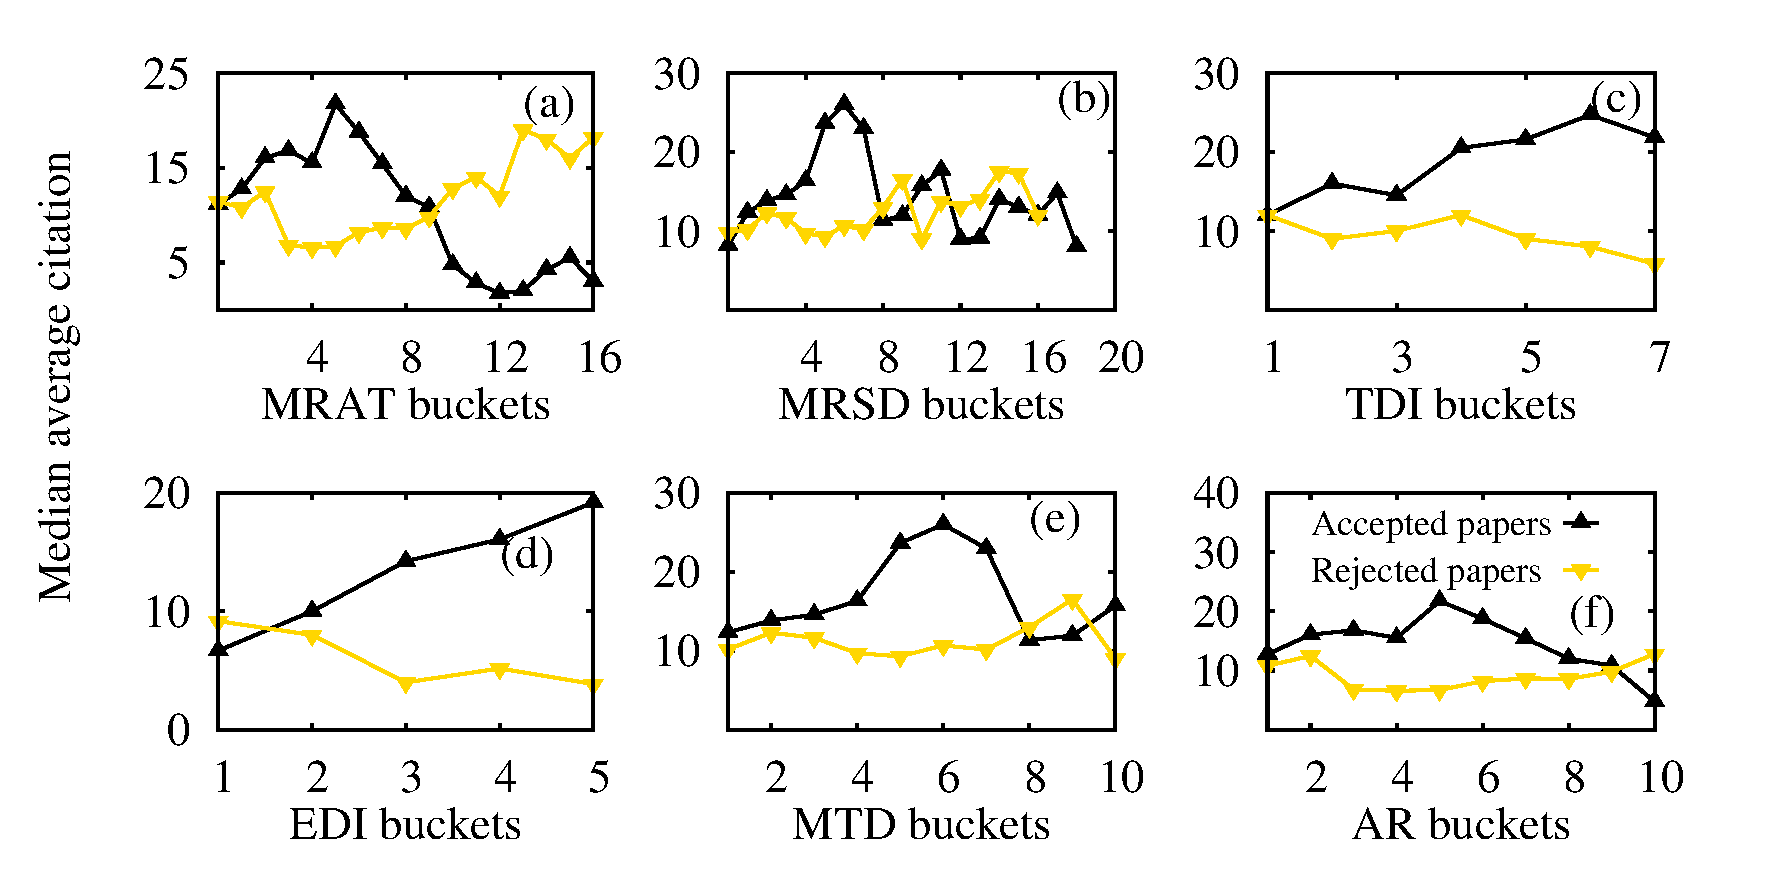
\includegraphics[width=0.9\textwidth]{./texfiles/Chapter_4/cikm/figures/reviewer_all.eps}
\caption{\label{fig5}(a) Median Average citation (MAC) versus $MRAT$. $MRAT$ values are bucketed into 20 buckets of equal size with range(1,498.8),(b) MAC versus $MRSD$ (c) MAC versus $TDI$, (d) MAC versus $EDI$, (e) MAC versus $MTD$ and (f) MAC versus $AR$. For both (c),(d) and (e), the x-axis values are bucketed by values corresponding to ($\geq$ 0 and $<$ 0.1), ($\geq$ 0.1 and $<$ 0.2) and so on. For (b) and (f) values (x-axis) are divided into 10 buckets of equal size.}
\end{figure}

We begin by analyzing the anomalous behavior of the editors. We define the behavior of an editor to be anomalous if the papers assigned to her are on average cited less when accepted or are cited more when rejected. In specific, we investigate different factors related to the editor that can lead to such anomaly.
\subsubsection{Mean Editor Assignment Time (MEAT)}
For each editor we obtain the time span (in days) between any two consecutive assignments and calculate the average time span between the two assignments. 
%The main objective is to check whether an editor who is assigned less frequently does a better job than an editor who is assigned more frequently. 
Formally, we define for editor $i$, $MEAT_{i}$ as
\begin{center}
$MEAT_{i}=\frac{1}{n-1}\sum (\delta_{j+1} - \delta_{j})$
\end{center}
where $n$ is the total number of assignments to the editor $i$ and $\delta_{j}$ is the date of the $j$$^\textrm{th}$ assignment. 
In figure~\ref{fig3}(a) we bin the editors based on the $MEAT$ and calculate the median average citation of the papers assigned to the editors in each bin. 
{We observe that for accepted papers very low or very high $MEAT$ values lead to lower citations. An exact opposite behavior is observed for rejected papers. 
This indicates that editors who are assigned time and again (low $MEAT$) or rarely (high $MEAT$) often fail to judge the quality of the papers assigned to them.} 
%Citation increases as $MEAT$ value increases which is then followed by decrease {\bf Not Clear} indicating that editors who are assigned very less frequently are also anomalous. 

\subsubsection{Self Review Index (SRI)}

%In many cases an editor assigns himself as a reviewer instead of assigning a different referee. While in some of these cases she could not find a reviewer (the reviewer declined), in many other cases she did not try to find a reviewer in the first place. 
{\bf Self Review Index (SRI)} measures the fraction of papers for which the editor assigned herself as the reviewer. 
Formally, for an editor $i$, we define $SRI_{i}$ as 
\begin{center}
$SRI_{i}=\frac{\varrho_{i}}{\rho_{i}}$
\end{center}
where $\rho_{i}$ is the number of papers $i$ was assigned as editor while $\varrho_{i}$ is the number of papers $i$ assigned herself as reviewer. We observe that with increasing values of $SRI$ the median average citation for accepted papers decreases while that for rejected papers increases (refer to figure \ref{fig3}(b)). 

\subsubsection{Referee-Author pair Diversity Index (RADI)}

We observe that editors in numerous cases assign papers from a certain author to only a certain reviewer. To investigate whether this allows for less impactful research from this author getting accepted, we define a metric which we call {\bf Referee-Author pair Diversity Index (RADI)}. Formally we define for editor $i$, the $RADI_{i}$ score as 

\begin{center}
$RADI_{i}=-\sum \limits_{j,k} p_{j,k} \log p_{j,k}$
\end{center}

where $p_{j,k}$ denotes the proportion of times a paper from author $k$ was assigned to reviewer $j$ by the editor $i$. In figure~\ref{fig3}(c) we bin the editors based on the $RADI$ and calculate the median average citation of the papers assigned to the editors in each bin. We observe that more the diversity score higher is the citation of the accepted papers and correspondingly lower is the citation of the rejected papers.


%[{\color{red}{\bf Check the last line; I have changed it. What you wrote earlier was not correct.}}]

\subsubsection{Referee Diversity Index (RDI)}
As a following step, we check whether an editor always chooses from a fixed set of reviewers or a diverse set of reviewers while making a paper assignment and, more importantly, does this influence the performance of the editor in terms of the impact of the reviewed paper. We define for each editor($i$) a metric called {\bf Referee Diversity Index ($RDI_{i}$)} as -  
%which assigns a diversity score for each reviewer depending on whether she selects from a diverse set of reviewers or a small fixed set while assigning. Formally for an editor $i$, $RDI_i$ is defined as
\begin{center}
$RDI_{i}=-\sum \limits_{j} p_{j}\log p_{j}$
\end{center}
where $p_{j}$ denotes the proportion of times reviewer $j$ was assigned a paper by editor $i$. More diverse the set of reviewers higher is the score. In figure~\ref{fig3}(b) we bin the editors based on the $RDI$ and calculate the median average citation of the papers assigned to the editors in each bin. We observe that more the diversity score, higher is the citation of the accepted papers and correspondingly lower is the citation of the rejected papers.

A summary statistic of all the above factors that may be used to identify anomalous editors are noted in Table~\ref{summary_stat}.

%\subsubsection*{Pathological cases}
The dataset allows us to find out the cases when the reviewer declined to review a paper on being assigned by an editor. We observe that editors with high $RDI$ are also declined more often. In figure~\ref{fig_sri}(b) we plot $RDI$ value and the number of declines for each editor. An increasing trend indicates that more diversely the editor tries to select reviewers more she gets declined by the reviewers. This in many cases may force the editor to be less proactive and always select from a specific set of `reliable' referees.  


%\noindent
\subsection{Analyzing reviewer tendencies}
\label{reviewer}
%\mycheckng{What percentage of reviewers are anomalous}
Reviewers are assigned with the responsibility of judging the quality of a submitted paper and hence their knowledge and training is highly critical. 
In fact, the decision of acceptance or rejection of a paper depends on the reviewer's perception of the paper. 

%\begin{figure}
% \centering
% \includegraphics[scale = 0.26]{figures/reviewer.eps}
% \caption{\label{reviewer} Cumulative distribution function of fraction of cases a reviewer was a part of a multi-referee system across all the reviewers
% for both JHEP and JSTAT datasets.}
%\end{figure}



%We calculate for each reviewer the fraction of cases where he is a part of a multi-referee set among his total assignments and plot the 
%cumulative distribution function of this fraction in figure~\ref{reviewer} for both JHEP and JSTAT datasets. The figure clearly indicates 
%that for JHEP the reviewers are mostly part of a single-referee set up while for JSTAT, the reviewers are part of a multi-referee set up in many more cases. 

% \begin{figure} 
%  \centering
%  \includegraphics[scale = 0.26]{figures/ed_ref_comb.eps}
%  \caption{\label{reviewer} Cumulative distribution function of the fraction of cases a reviewer is a part of a multi-referee system across all the reviewers for JHEP and JSTAT datasets.}\end{figure}
\begin{figure}
 \centering
 \includegraphics[scale = 0.3]{./texfiles/Chapter_4/cikm_17/figures/citation_delay_acpt_ratio_jhep.eps}
 \caption{\label{a_d_jhep} Mean citation versus (a) accept ratio (b) assignment delay buckets for the JHEP dataset. 
 Note that the papers are segregated into accept ratio/delay bins and the mean citation is calculated for each bin. 
 Typical bin sizes for accept ratio are $<0.1$,$(\geq 0.1$ and $<0.2)$ and so on while for delay the sizes are $<100$, $(\geq 100$ and $< 200)$ and so on.\vspace{4mm}}
\vspace{3mm}
 \end{figure}

%We further leverage the technique introduced in~\cite{sikdar2016anomalies} and identify the set of under-performing
% reviewers for both the datasets. 
% \mycheck{put in the definition of underperforming/anomalous-----}
In the last section we defined a referee/editor to be anomalous (under-performing) if - \\
(i) papers accepted by him/her have low citation (research wrongly judged to be impactful)\\
(ii) papers rejected by him/her have high citation (quality research wrongly judged as flawed)\\
%In fact, the authors propose a method for identifying under-performing (anomalous) referees/editors. Leveraging on the same method we observe that  
% the proportion of referees classified as under-performing are approximately $26\%$ and $21\%$ respectively for JHEP and JSTAT datasets.
%The authors hypothesize that accepted papers receiving low citation as well as rejected papers receiving high citations are anomalous cases as 
%ideally they should have been respectively rejected and accepted.  
We make the following general observations - \\
(i) If we consider all the cases where an under-performing editor assigned multiple reviewers for a submission, in $69.8\%$ cases 
at least one of them was under-performing. This indicates that unless the reviewers are selected carefully, chances are it might lead to wrong judgment.\\
(ii) Under-performing reviewers when part of a multi-referee system tend to do a better judgment as compared to cases when they serve as single reviewers.
This is illustrated by the fact that average citation of the accepted  papers reviewed by multiple reviewers with at least one under-performing reviewer ($32.4$) 
is more compared to that of the papers reviewed by a single anomalous reviewer ($18.2$) across the two datasets.
%\vspace{-4mm}
\subsubsection{Factors determining performance of the referees}
We next look into factors that could be used to quantify the performance of the reviewers. The quantification can be used as a 
fitness value for assignment of a new submission (we use these to calculate these quantities in a later section to develop a scheme for automatic referee group selection). 
Given a submission, we identify two factors that are indicative of reviewer fitness (i) accept ratio and (ii) time since the last assignment.\\
\noindent(i) \textit{Accept ratio}: Given a submission, we consider for each reviewer ($i$) the fraction of papers (s)he has accepted at the time of submission. 
We denote this by $a_i$. To show that it is indeed an indicator we consider all the accepted and the rejected papers as well as their assigned reviewers. 
We then calculate the accept ratio of the assigned reviewers and compare them against the citations received by each of them. 
In figures~\ref{a_d_jhep}(a) (JHEP) and~\ref{a_d_jstat}(a) (JSTAT) we plot the accept ratio against the citations received by the accepted as well as the rejected papers. 
Note that we bin the papers based on the accept ratio and calculate the average citation in each case. The typical bin sizes are $\leq 0.1$, $(> 0.1$ and $\leq 0.2)$ and so on. 
We hence obtain $10$ such bins numbered 1-10. 
In case of multi-referee papers the average accept ratio of the reviewers is considered. We observe that for both the datasets very high accept ratio or a very low accept 
ratio might lead to wrong judgment. \\ 
\noindent(ii) \textit{Time since last assignment}: Given a submission and its corresponding submission date we calculate for each reviewer ($i$) the time (in days) between the 
last review assignment date and the submission date (denoted by $d_i$). To illustrate the rationale, we again consider all the accepted and the rejected papers and calculate 
the delay for the assigned reviewers. We again bin the delay values and calculate the average citation (refer to figures~\ref{a_d_jhep}(b) and~\ref{a_d_jstat}(b)). Typical bin 
sizes are $\leq 100$, $(> 100$ and $\leq 200)$ and so on (10 such bins are obtained numbered 1-10). We observe that the reviewers who are assigned very close to their last 
assignment or those who have not been assigned for a long time often fail to correctly judge the quality of the paper correctly as the papers accepted by them are cited less 
on average while those rejected are cited more. 


% \begin{figure}
%  \centering
%  \includegraphics[scale = 0.26]{figures/citation_delay_acpt_ratio_jhep.eps}
%  \caption{\label{a_d_jhep} Mean citation versus (a) accept ratio (b) assignment delay buckets for the JHEP dataset. 
%  Note that the papers are segregated into accept ratio/delay bins and the mean citation is calculated for each bin. 
%  Typical bin sizes for accept ratio are $<0.1$,$(\geq 0.1$ and $<0.2)$ and so on while for delay the sizes are $<100$, $(\geq 100$ and $< 200)$ and so on.}
% \end{figure}

\begin{figure}
 \centering
 \includegraphics[scale = 0.3]{./texfiles/Chapter_4/cikm_17/figures/citation_delay_acpt_ratio_jstat.eps}
 \caption{\label{a_d_jstat} Mean citation versus (a) accept ratio (b) assignment delay buckets for JSTAT dataset. Note that the papers are 
 segregated into accept ratio/delay bins and the mean citation is calculated for each bin. Bin sizes are same as figure \ref{a_d_jhep}.\vspace{4mm}}
\vspace{3mm}
 \end{figure}



\subsubsection{Action with under-performing reviewers}
A naive solution could be to not assign the under-performing reviewers and only assign the best performing ones, but this is not always feasible 
since the number of referees is limited and they often decline assignments. Hence a better solution would be to group them such that the overall performance improves. 
To this aim, we first divide the reviewers into 3 classes separately for accept ratio and time 
since last assignment. A reviewer $i$ with accept ratio $a_i < 0.3$ is assigned ``Low'' (L), with $0.3 \leq a_i < 0.6$ is assigned ``Medium'' (M) and with $a_i \geq 0.6$ is 
assigned ``High'' (H). Note that reviewers in M were the best performing referees (refer to figures \ref{a_d_jhep}(a) and \ref{a_d_jstat}(a)). Each multi-refereed paper 
(by exactly 2 referees) is classified into one of the six classes (LL, MM, HH, LH, MH, LH) based on the class of each referee and the average citation of the papers in each 
class is noted (figure \ref{ref_perf}(a)). We observe that when both the referees belong to the M class (MM) the performance is naturally well. More importantly, reviewers in L and H class 
perform better when paired with a referee from M class (even better than MM). On repeating the same experiment with time since last assignment, 
we observe a similar trend (figure \ref{ref_perf}(b)) with MM class performing the best followed by MH and LM.  
Note that in this case reviewers with $d_i < 100$ are assigned class L, with $100 \leq d_i < 300$ are assigned M and rest are assigned H. 
%This indicates that grouping 
%reviewers while assigning multiple referees for a 
%submission is highly critical toward improving the effectiveness of the system. 
%We further look into the proportion of discordant cases for each reviewer combination. 
More importantly the discordant cases mostly occur for 
class combinations LL, HH and LH (refer to table \ref{tab:dis}). In fact, MM has the least proportion of discordant cases. 
This further indicates the correct reviewer grouping is critical in curtailing the discordant cases which is one of the prime reasons behind the multi-reviewer system failing. 
Note that the above results are obtained for JHEP dataset and a similar pattern is observed 
for JSTAT as well.

\begin{figure}
 \centering
 \includegraphics[scale = 0.3]{./texfiles/Chapter_4/cikm_17/figures/ref_performance.eps}
 \caption{\label{ref_perf} Mean citation for papers belonging particular class combination with respect to (a) accept ratio (b) time since last assignment. For example LL would represent a paper reviewed by referees both 
 belonging to class L.\vspace{4mm}}
\end{figure}







\medskip


\subsection{Reviewer}
\label{reviewer}

In this section, we investigate anomalous behavior of the referees. Recall that we define the behavior of a reviewer to be anomalous if the papers accepted by her are low cited or the papers rejected by her are highly cited. As in case of the editors, here also we investigate different factors that could be indicative of such anomalous behavior.  

\subsubsection{Mean Reviewer Assignment Time (MRAT)}

%For each individual reviewer we find the time difference (in days) between two consecutive assignments. Note that we do not consider the cases where the reviewer was assigned but she declined to review it.
This is essentially same as MEAT. For a reviewer $i$, we define $MRAT_{i}$ as
\begin{center}
$MRAT_{i}=\frac{1}{n-1}\sum (\delta_{j+1} - \delta_{j})$
\end{center}
\noindent where $n$ is the total number of assignments of reviewer $i$ and $\delta_{j}$ is the date of the $j^\textrm{th}$ assignment. In figure~\ref{fig5}(a) we plot $MRAT$ (binned) and median average citation of the papers reviewed for each reviewer. We observe that papers reviewed by reviewers with low $MRAT$ (high frequency of assignment) tend to be cited less and increases as $MRAT$ increases. This is followed by again a steep decrease in citation. This indicates that the reviewers assigned very frequently are often less reliable while those assigned only occasionally are also not likely to correctly judge the quality of the paper.  

\subsubsection{Mean Report Sending Delay (MRSD)}

We argue that the time taken by a reviewer to send back the review report could be an indicator of his performance. If a reviewer on average sends back the review very quickly it is highly likely that the review was done in a hurry. Similarly, if the report was sent after being reminded by the editor numerous times, it is also highly likely the review report could be anomalous. For a reviewer we calculate the time delay between the date of her assignment and the date she sent back the report for each of her assignments. To measure $MRSD$ we calculate the mean value of all the delays. Note that we do not consider the assignments which the reviewer declined. Formally, for a reviewer $i$, we define $MRSD_{i}$ as 

\begin{center}
$MRSD_{i}=\frac{1}{n}\sum(\delta_{i}-\Delta_{i})$
\end{center}

where $n$ is the total number of assignments, $\Delta_{i}$ is the date of assignment and $\delta_{i}$ is the date when the report was received by the editor. On plotting against median average citation we observe a similar trend as was observed in case of $MRAT$ (refer to figure~\ref{fig5}(b)). Papers reviewed by reviewers with low $MRSD$ value are often less cited, indicating that reviewers sending back their report very quickly often do it in a hurry and fail to correctly judge the quality of the paper while those taking very long to send report are prone to failure as well. 

\subsubsection{Topic Diversity Index (TDI)}

JHEP associates with each submission a set of keywords which roughly indicates the domain of the work. We use these associated keywords as a proxy for topic. For each reviewer, we segregate all the keywords of the papers reviewed by her which we call the keyword corpus for the reviewer. Formally for a reviewer $i$, we define $TDI_{i}$ as 

\begin{center}
$TDI_{i}=-\sum \limits_{j} p_{j}\log p_{j}$
\end{center}

\noindent where $p_{j}$ is the proportion of keyword $j$ in the keyword corpus for reviewer $i$. We segregate the reviewers based on the diversity score and calculate the median average citation of the papers reviewed by them. We observe that the median average citation %[{\color{red}{\bf Why introduce this acronym here? Use it from the first time it has been invoked.}}] 
for reviewers with low $TDI$ are low mainly because the number of papers reviewed by them are also less. The value increases with  increasing $TDI$ (refer to figure~\ref{fig5}(c)). The reviewers with low $TDI$ are often the ones who have reviewed a very small number of papers while the reviewers with high $TDI$ are mostly assigned papers by a large number of editors. 
 
 
 
\subsubsection{Editor Diversity Index (EDI)}

Reviewers could be selected for review by a large set of editors or could only be selected by a single or a small set of editors. We check whether a reviewer selected by many editors is more reliable compared to one who is selected by a single or a very small set of editors. To this aim we assign each reviewer a score called Editor Diversity Index, $EDI_{i}$ which is defined as 

\begin{center}
$EDI_{i}=-\sum \limits_{j} p_{j}\log p_{j}$
\end{center}

where $p_{j}$ represents the proportion of times reviewer $i$ was assigned by editor $j$. We segregate the reviewers based on $EDI$ and calculate the median average citation of the papers reviewed by them. We observe that as $EDI$ increases median average citation also increases (refer to figure \ref{fig5}(d)) indicating that reviewers assigned by multiple editors are often more reliable.

\begin{table}[htpb]
\centering
\caption{Features used for detecting anomalies.}
\label{summary_stat}
\small
\begin{tabular}{|l|l|l|l|l|l|l|}
\hline
                        & Factor                                     & Mean & Median & Max & Min & \begin{tabular}[c]{@{}l@{}}St.\\ Dev\end{tabular} \\ \hline
\multirow{3}{*}{Editor} & $MEAT$         & 35.06     &  29.1      &  108.25   &  3.28   & 23.19                                                             \\  
                        & $RDI$              & 6.57     &  6.79      & 8.85    & 0.0    &  1.44                                                            \\ 
                        & $RADI$ & 8.86     & 9.21       & 11.94    & 0.0    &  1.87 
                         \\ 
                        & $SRI$ & 0.28     & 0.25       & 0.85    & 0.0    &  0.19                                                           
                        \\ \hline
\multirow{6}{*}{Reviewer} & $MRAT$       & 363.3     & 193.7       & 5389    & 26.9    & 508.9                                                             \\  
                        & $MRSD$           & 19.28     & 17.50       & 122    & 16.5    &  11.45                                                            \\  
                        & $TDI$                &  4.07    &  3.96      & 8.10    & 1.0    &  1.44                                                            \\  
                        & $EDI$               &  1.12    &   0.91     &  4.58   & 0.0    &   1.19                                                           \\  
                        & $AR$                      &  0.65    &   0.71     &   1.0  & 0.0    &    0.2                                                          \\  
                        & $MTD$                 &   3.86   &  3.12      & 69.0    & 1.0    & 4.96                                                             \\ 
                        & $DFI$                 & 0.19     & 0.12       & 1.0    & 0.0    & 0.30                                                             \\ \hline
                        
\end{tabular}
\end{table} 


\subsubsection{Mean Time to Decline (MTD)}

We further investigated the cases where the reviewer declined the assignment. In specific, we calculated the time delay (in days) 
between the date she was assigned and the date she conveyed her decision of declining to review. For each reviewer we define {\bf Mean Time to Delay}, $MTD_{i}$ as 

\begin{center}
$MTD_{i}= \frac{1}{d}\sum \limits_{j}(\mu_{j} - \Delta_{j})$
\end{center}

where $d$ is the number of assignments that reviewer $i$ declined and $\mu_{j}$ and $\Delta_{j}$ are respectively the date of assignments and date of reply for paper $j$ by reviewer $i$. We segregate the reviewers based on their $MTD$ values and calculate the median average citation. We observe that the reviewers who delay often in reporting their decision to the editor of being unable to review usually tend to fail in judging a paper quality when they do review (refer to figure~\ref{fig5}(f)).

\subsubsection{Acceptance Ratio (AR)}
Acceptance Ratio ($AR$) of a reviewer is defined as the proportion of papers accepted by the reviewer. For a reviewer $i$, $AR_{i}$ is formally defined as 

\begin{center}
$AR_{i}=\frac{a_{i}}{a_{i}+r_{i}}$
\end{center}

\noindent where $a_{i}$ and $r_{i}$ respectively denote the number of papers accepted and rejected by reviewer $i$. We observe that reviewers with high $AR$ often accept  less impactful papers while reviewers with very low $AR$ often fail to identify quality research (refer to figure~\ref{fig5}(e)). Note that the reviewers are segregated based on their respective $AR$ values while the median average citation is calculated. They are segregated into bins based on the $AR$ values where typically the bins are ($\geq$ 0 and $< 0.1$), ($\geq$ 0.1 and $<$ 0.2) and so on.

\begin{figure}
\centering
\includegraphics[scale=0.4]{./texfiles/Chapter_4/cikm/figures/DFI_dec_month.eps}
\caption{\label{fig_dfi}(a) Median Average citation versus $DFI$. $DFI$ values are bucketed by values corresponding to ($\geq$ 0 and $<$ 0.1), ($\geq$ 0.1 and $<$ 0.2) and so on. (b) Number of declines versus the month of the year.}
%\vspace{-.4cm}
\end{figure}
%begin{figure}
%ncludegraphics[scale=0.22]{figures/decline_month.eps}
%aption{\label{fig6} Number of declines versus the month of the year.}
%end{figure}

\subsubsection{Decline Fraction Index (DFI)}

{\bf Decline Fraction Index (DFI)} for a reviewer is the fraction of times she declined to review. For a reviewer $i$, we define $DFI_{i}$ as
\begin{center}
$DFI_{i}=\frac{\vartheta_{i}}{\theta_{i}}$
\end{center}

\noindent where $\theta_{i}$ is the total number of assignments while $\vartheta_{i}$ is the number of times $i$ declined to review. 
In figure \ref{fig_dfi}(a) we plot median average citation versus $DFI$. We observe that for accepted papers the citation is higher for lower $DFI$ values and it drops as $DFI$ increases indicating that reviewers declining too frequently often fail to judge the quality of the paper assigned to them.

A summary statistics of all the above factors that may be used to identify anomalous referees are noted in Table~\ref{summary_stat}.

%\subsubsection*{Pathological Cases}
We further looked into the data and made some interesting observations which are summarized below - \\
(i) A bulk of the instances where a reviewer declined to review occurred in the month of July and August. This is represented in figure~\ref{fig_dfi}(b). This probably relates to the vacation time in the Europe and the US.
(ii) Of the 4035 reviewers 756 of the reviewers have not been assigned a paper for the last two years. On further investigation we observed that among these there are 505 such reviewers who in their immediate last review assignment agreed to review but did not send back the report.


%\noindent
\subsection{Identifying anomalous Editors and Reviewers}
\label{prediction}

%[{\color{red}{\bf Shall ckeck the rest from here after you have a complete version.}}]

In the previous sections we discussed how different factors indicate anomalous behavior of referees and editors. In this section, we check whether we can use them to automatically differentiate between normal and anomalous editors and referees. We propose separate unsupervised models for editors and reviewers.

\begin{figure}
\centering
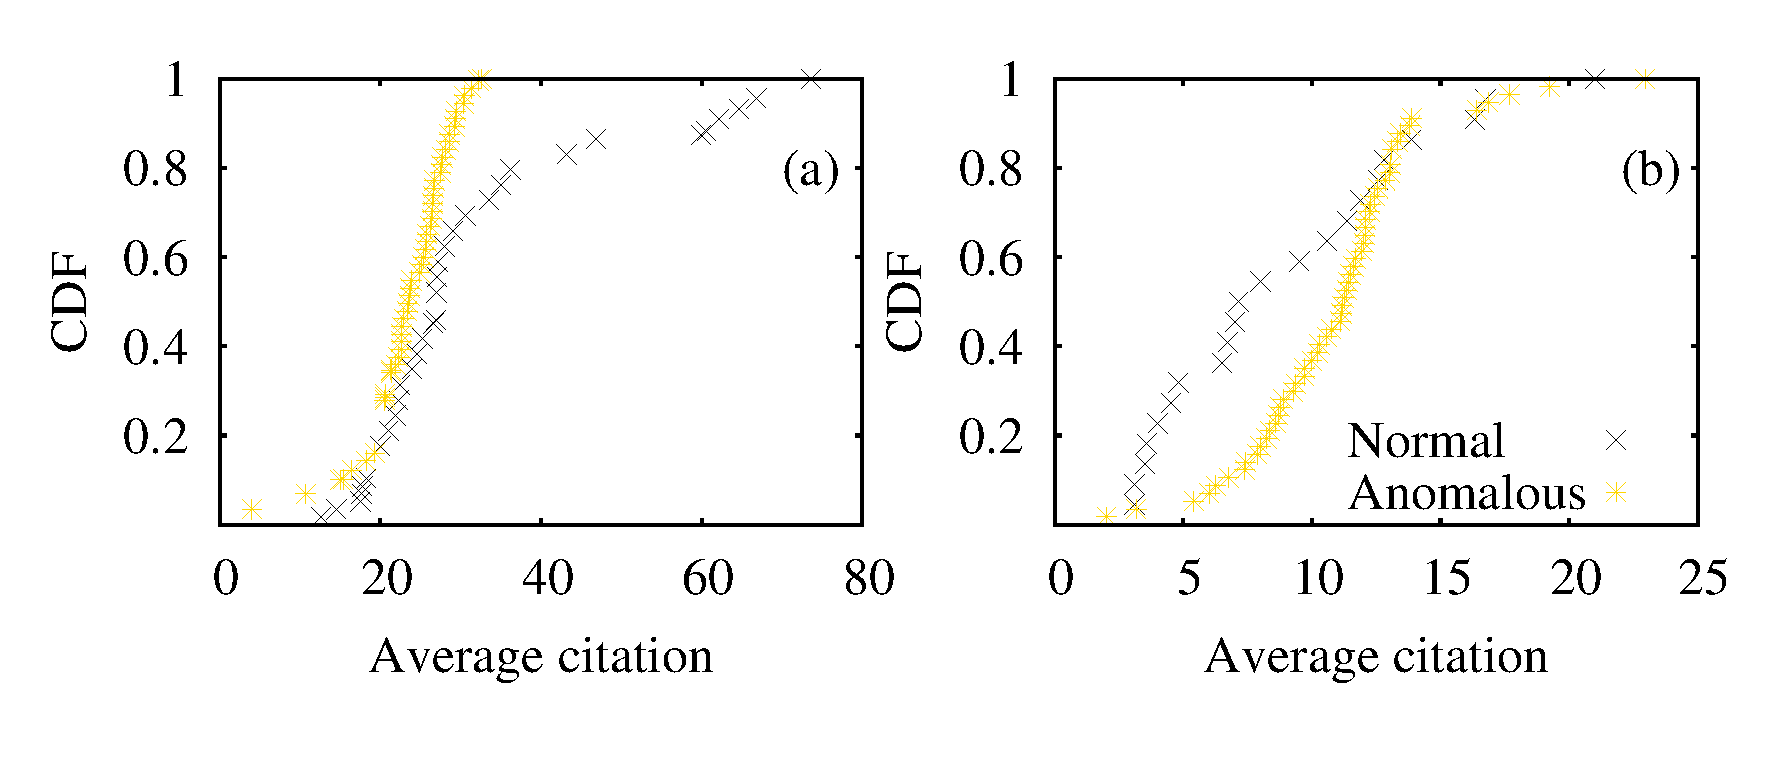
\includegraphics[scale=0.27]{./texfiles/Chapter_4/cikm/figures/editor_all_anom.eps}
\caption{\label{ed_pred}Cumulative distribution function of the average citations for the two sets of editors (anomalous and normal).\vspace{4mm}} 
\end{figure}


\subsubsection{Editors}
For each editor $i$, we measure $MEAT_{i}$, $RDI_{i}$, $RADI_{i}$ and $SRI_{i}$ which form a feature vector. 
%[{\color{red}{\bf Have you not used $SRI$? Why?}}] 
We also consider the editors who were assigned at least 5 papers and accepted at least 1 paper before 2013. 
To detect anomalies we use the 
$k-means$ clustering setting with $k=2$. The two clusters are of sizes 25 and 68 respectively. Clearly this set of 25 editors are the anomalous ones.
In figure \ref{ed_pred} we plot the cumulative distribution of average citation of accepted (figure \ref{ed_pred}(a)) and rejected  (figure \ref{ed_pred}(b)) papers. We observe that citation of accepted papers assigned to anomalous editors are significantly lower while citation of rejected papers are significantly higher compared to those assigned to normal editors.


\subsubsection{Reviewers}

Similarly for each reviewer $i$ we associate a feature vector of size seven consisting of $MRAT_{i}$, $MRSD_{i}$, $TDI_{i}$, $EDI_{i}$, $AR_{i}$, $MTD_{i}$ and $DFI_{i}$. 
%[{\color{red}{\bf Have you not used $DFI$? Why?}}] 
We filter out reviewers who have reviewed at least 5 papers and accepted at least 1 before 2013. This reduces our set of reviewers to 2328. By using $k-means$ clustering ($k=2$), we obtain two clusters of size 339 and 
1999. On plotting cumulative distribution of the average citation for accepted (refer to figure \ref{rev_pred}(a)) and rejected papers (refer to figure \ref{rev_pred}(b)), we observe that the papers accepted by anomalous reviewers are cited significantly lesser while those rejected by them are cited significantly higher compared to the normal referees.

\begin{figure}
\centering
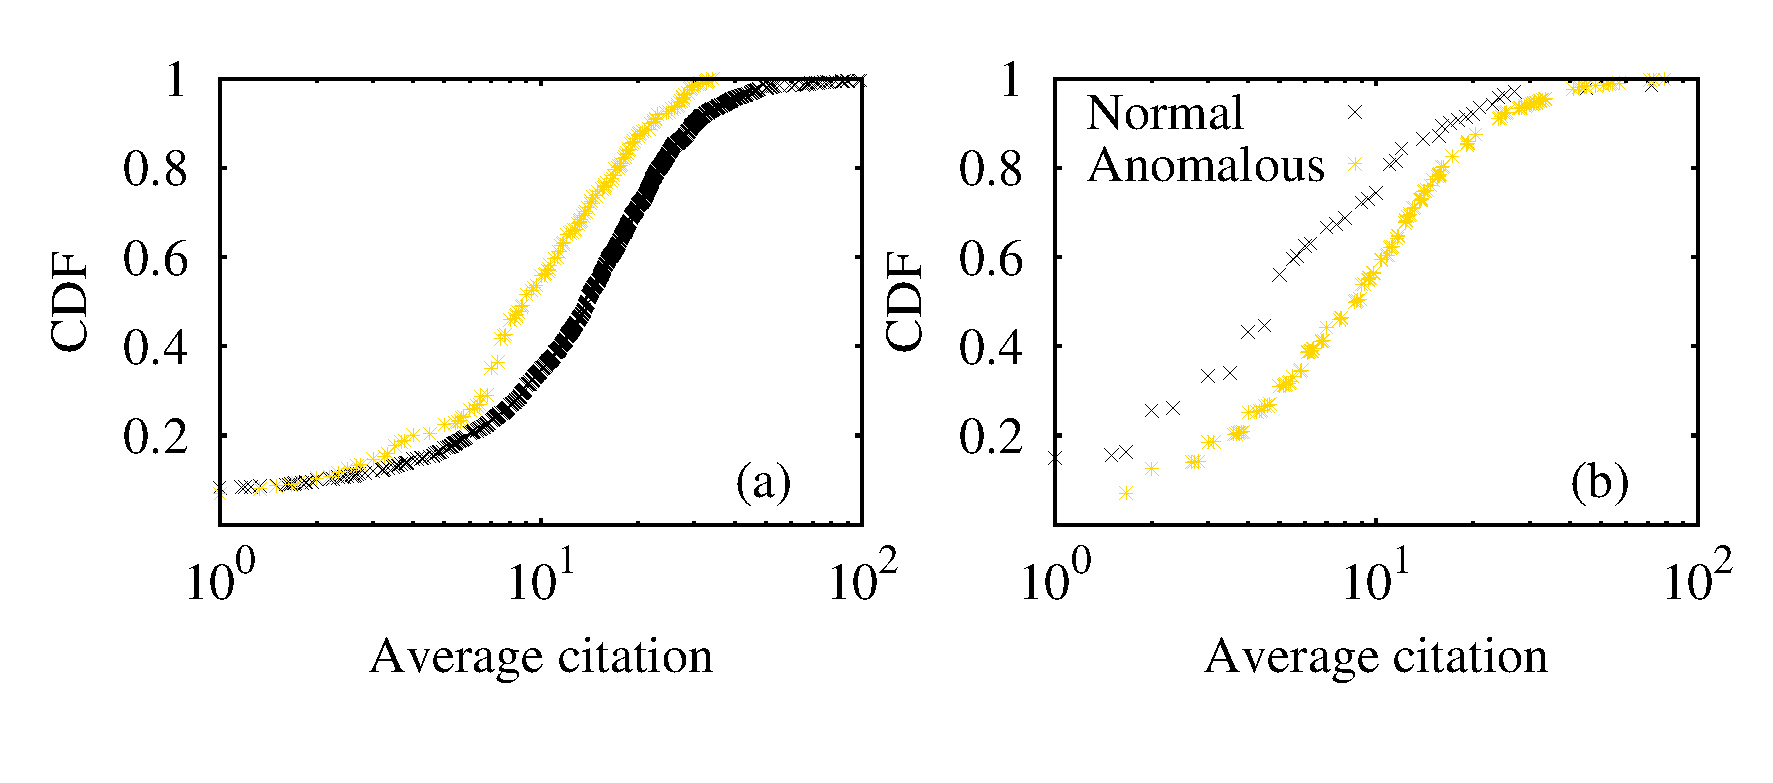
\includegraphics[scale=0.27]{./texfiles/Chapter_4/cikm/figures/reviewer_all_anom.eps}
\caption{\label{rev_pred}Cumulative distribution function of the average citations for the two sets of reviewers (anomalous and normal).\vspace{4mm}}
\vspace{3mm}
\end{figure}
%Thus, using the above features we were able to identify the anomalous reviewers and editors. We believe our method could be useful in further improving the peer-review process. Moreover it could be useful in assisting editors to select reviewers as well as administrators in selecting editors. 
\medskip

\section{Identifying anomalous Editors and Reviewers}
\label{prediction}

%[{\color{red}{\bf Shall ckeck the rest from here after you have a complete version.}}]

In the previous sections we discussed how different factors indicate anomalous behavior of referees and editors. In this section, we check whether we can use them to automatically differentiate between normal and anomalous editors and referees. We propose separate unsupervised models for editors and reviewers.

\begin{figure}
\centering
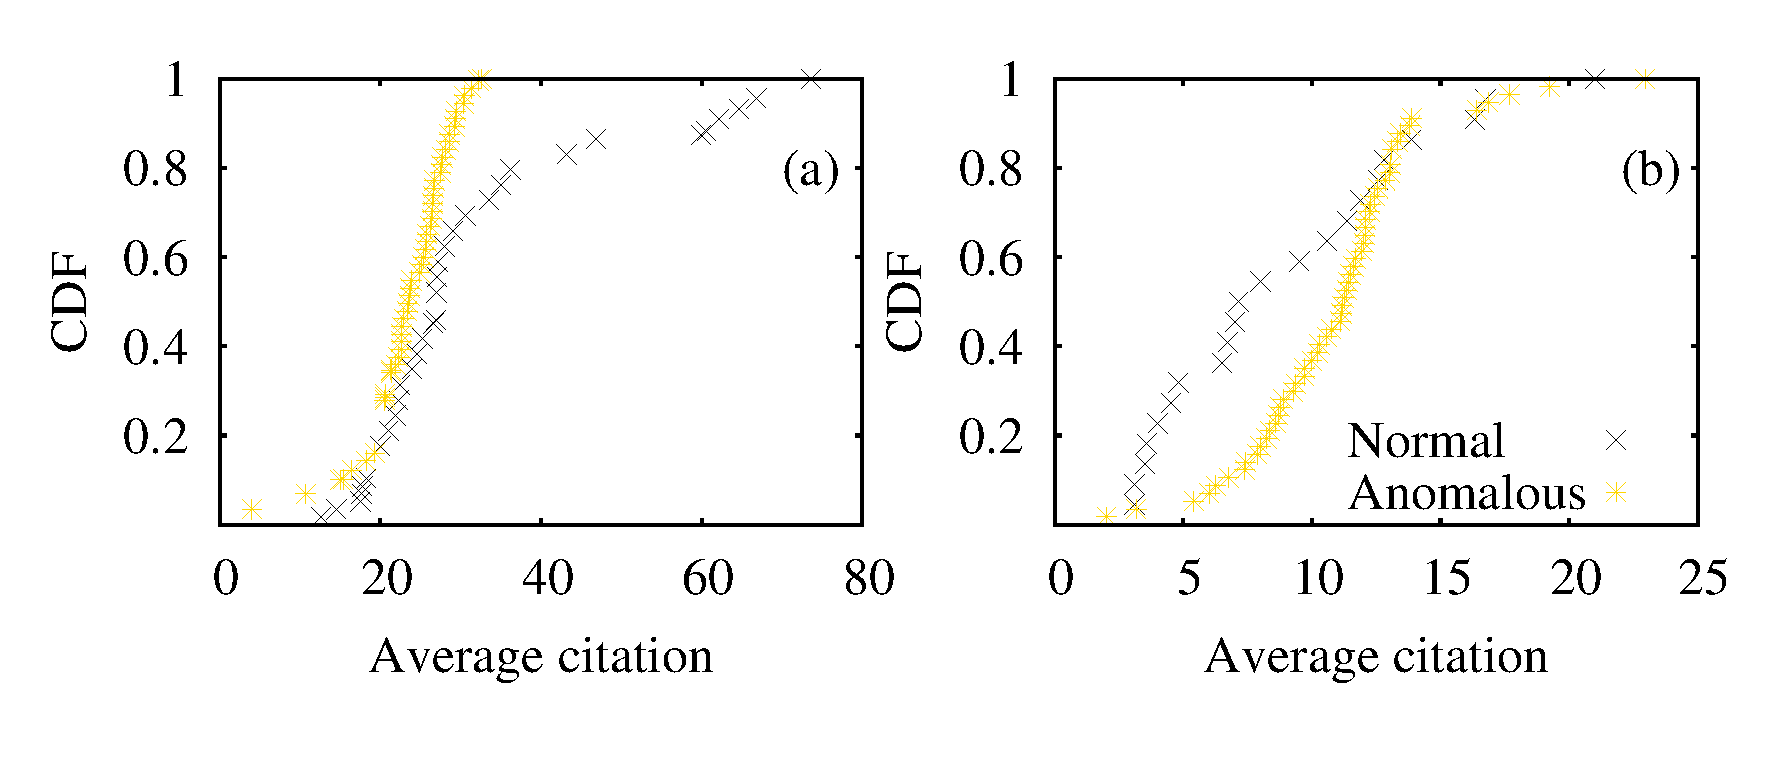
\includegraphics[scale=0.27]{./texfiles/Chapter_4/cikm/figures/editor_all_anom.eps}
\caption{\label{ed_pred}Cumulative distribution function of the average citations for the two sets of editors (anomalous and normal).} 
%\vspace{-.4cm}
\end{figure}


\subsection{Editors}
For each editor $i$, we measure $MEAT_{i}$, $RDI_{i}$, $RADI_{i}$ and $SRI_{i}$ which form a feature vector. 
%[{\color{red}{\bf Have you not used $SRI$? Why?}}] 
We also consider the editors who were assigned at least 5 papers and accepted at least 1 paper before 2013. 
To detect anomalies we use the 
$k-means$ clustering setting with $k=2$. The two clusters are of sizes 25 and 68 respectively. Clearly this set of 25 editors are the anomalous ones.
In figure \ref{ed_pred} we plot the cumulative distribution of average citation of accepted (figure \ref{ed_pred}(a)) and rejected  (figure \ref{ed_pred}(b)) papers. We observe that citation of accepted papers assigned to anomalous editors are significantly lower while citation of rejected papers are significantly higher compared to those assigned to normal editors.


\subsection{Reviewers}

Similarly for each reviewer $i$ we associate a feature vector of size seven consisting of $MRAT_{i}$, $MRSD_{i}$, $TDI_{i}$, $EDI_{i}$, $AR_{i}$, $MTD_{i}$ and $DFI_{i}$. 
%[{\color{red}{\bf Have you not used $DFI$? Why?}}] 
We filter out reviewers who have reviewed at least 5 papers and accepted at least 1 before 2013. This reduces our set of reviewers to 2328. By using $k-means$ clustering ($k=2$), we obtain two clusters of size 339 and 
1999. On plotting cumulative distribution of the average citation for accepted (refer to figure \ref{rev_pred}(a)) and rejected papers (refer to figure \ref{rev_pred}(b)), we observe that the papers accepted by anomalous reviewers are cited significantly lesser while those rejected by them are cited significantly higher compared to the normal referees.

\begin{figure}
\centering
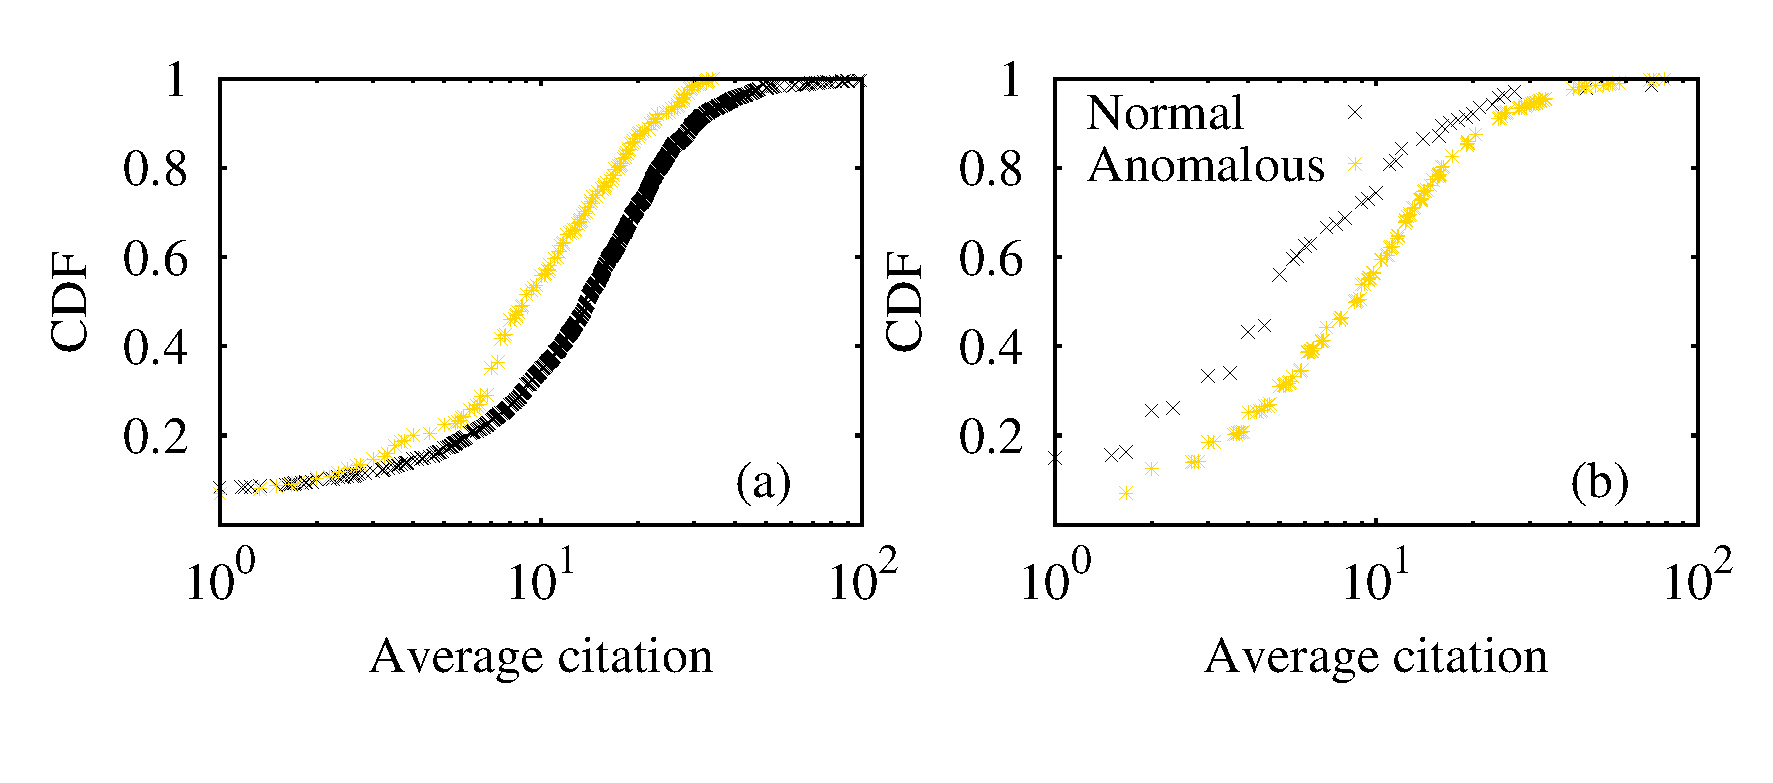
\includegraphics[scale=0.4]{./texfiles/Chapter_4/cikm/figures/reviewer_all_anom.eps}
\caption{\label{rev_pred}Cumulative distribution function of the average citations for the two sets of reviewers (anomalous and normal).}
%\vspace{-.4cm}
\end{figure}


%\begin{figure}
\centering
\includegraphics[scale=0.25]{./texfiles/Chapter_4/jcdl/figures/len_citation.eps}
\caption{Mean length of referee reports in terms of number of words at different rounds of review. Typically the buckets are $< 100$, ($\geq 100, < 200$) and so on}
\label{fig:length}
\end{figure}


\subsection{Review report based features}
\label{text_analysis}

In this subsection we analyze whether certain features could be extracted from the reports sent by the reviewers that could be an indicator of the long-term citation of the paper. Note that we have two types of reports -- {\bf Referee report}: Report sent by the assigned referee to the editors and {\bf Editor report}: Report sent by the editor to the authors based on the referee report. We primarily focus on the referee reports as editorial reports are in almost all cases a reiteration of the referee reports.

\subsubsection{Length of the reports (RL)}
We start by looking whether the length of the review reports sent by the reviewers are indicative of the quality and hence the long-term citation of the paper. To this aim we segregate the papers based on the length of the report and calculate the mean citation of each of these buckets. The lengths are bucketed with sizes typically $< 100$, ($\geq 100, < 200$) and so on. We observe that there exists an optimal length (between 500 and 600 words) for which the citation obtained by the corresponding paper is maximum  (refer to figure \ref{fig:length}). 


\subsubsection{Sentiments (SNT)}
We next perform sentiment analysis on the review reports. To determine the sentiment of a report we use a method described in~\cite{montejo2012random} which performs a graph-based word sense disambiguation and lexical similarity analysis using a pre-existing knowledge base. A sentiment score of 0 indicates that the document is neutral, a positive score  indicates a positive sentiment and a negative score indicates a negative sentiment. 


\begin{figure}[htpb]
\centering
%\vspace{-5mm}
\includegraphics[scale=0.23]{./texfiles/Chapter_4/jcdl/figures/year_sent_cit-eps-converted-to.pdf}
\caption{Sentiment score versus citations for both accepted and rejected papers for the years 2005, 2007 and 2009. We find similar trends for other years as well.}
\label{fig12}
\end{figure}

To determine whether the overall sentiment of the reviews of a paper is related to the number of citations received by it, we plot for each paper (both accepted and rejected) the number of citations it received against the  sentiment score of the first round of review in fig.~\ref{fig12}. Note that we segregate the papers based on the year of the publication or the rejection. We observe that the highly cited papers mostly have reviews with neutral or positive sentiment. Accepted papers with positive reviews are, on average, found to receive $25.27$ citations while those with negative reviews are found to receive $13.56$ citations.
However, there are cases where the accepted paper received highly positive reviews but was not cited. Conversely, there are cases where the sentiment was neutral but the paper garnered a large number of citations. Shown below are two such examples -- {\bf Case 1:} Year of publication: 2006, sentiment score: 0.0234 (almost neutral), citations: 5812; {\bf Case 2:} Year of publication: 2008, sentiment score: 0.65 (highly positive), citations: 6.


For the rejected papers we observe that those which received neutral reviews but were rejected, tend to garner higher citations later compared to the ones which received negative reviews. There are certain exceptions as well, two of which are -- {\bf Case 1:} Year of rejection: 2010, sentiment score: 0.27 (positive), citations: 1; {\bf Case 2:} Year of rejection: 2007, sentiment score: -0.14 (negative), citations: 711.
Manual investigation of the review text shows that the papers which are highly cited after rejection were mainly rejected for not being in the scope of JHEP and not because of flawed results. 

\subsubsection{Linguistic quality indicators (LQI)}

Here we check whether there are linguistic quality features present in the review reports which can serve as an indicator of the future impact of the paper. To our aim we use the LIWC\footnote{\url{http://liwc.wpengine.com/}} (Linguistic Inquiry and Word Count) text analysis tool~\cite{pennebaker2007development}. The tool provides, as output, percentage of words in different categories for an input text. The categories are broadly divided into linguistic (21 dimensions like pronouns, articles etc.), psychological (41 dimensions like affect, cognition etc.), personal concern (6 dimensions), informal language markers and punctuation apart from some general features like word count, words per sentence etc. We apply the LIWC tool on the review reports for our analysis and mainly focus on the linguistic and the psychological categories.
Next we check whether the LIWC features discussed earlier can also serve as indicators differentiating high and low cited papers. We rank the papers based on the number of citations they have received and consider the top 10\% as highly cited and the bottom 10\% as low cited papers. Note that we only consider the papers that were published before 2012 so that the papers have at least three years of citation history. In table~\ref{tab3} we report the mean percentage of words in different LIWC categories across all the papers (both high and low cited). We find several quality indicators here as well. The key observations are: (i) future tense is used more significantly in case of review reports of highly cited papers compared to low cited papers. On manually investigating the reviews of some of the highly cited papers we observe that statements like ``its result will become a useful addition to ..'' are prevalent; (ii) insightful and inclusive words are also used to a greater extent in review reports of highly cited papers compared to low cited papers; (iii) positive words are also more prevalent in highly cited papers as well.\\
Thus, these indicators show that the reviewers were, in many cases, indeed able to guess the quality of the paper as is evident from the review reports.

\begin{table}
\centering
\caption{Mean values of percentages of various categories of words in review reports of high and low cited papers where the means differ significantly.\vspace{3mm}}
\label{tab3}
\begin{tabular}{|l|l|l|l|}
\hline
Category                    & Dimension                                                   & \begin{tabular}[c]{@{}l@{}}High cited\\ papers\end{tabular} & \begin{tabular}[c]{@{}l@{}}Low cited\\ papers\end{tabular} \\ \hline \hline
\multirow{2}{*}{Linguistic} & Future tense                                                & 1.17                                                          & 1.05                                                         \\ \cline{2-4} 
                            & Negation                                                    & 0.72                                                          & 0.84                                                         \\ \hline
\multirow{4}{*}{Cognitive}  & Insight                                                     & 3.52                                                          & 3.16                                                         \\ \cline{2-4} 
                            & Causation                                                   & 2.60                                                          & 2.38                                                         \\ \cline{2-4} 
                            & Inclusive                                                   & 3.70                                                          & 3.43                                                         \\ \cline{2-4} 
                            & Exclusive                                                   & 1.28                                                          & 1.52                                                         \\ \hline
Affective                   & \begin{tabular}[c]{@{}l@{}}Positive \\ emotion\end{tabular} & 2.84                                                          & 2.70                                                         \\ \hline
\end{tabular}
\vspace{2mm}
\end{table}


%\noindent
\section{Profiling Anomalous Reviewers}
\label{profile}


In this section we analyze in more details the performance of the anomalous reviewers. To this aim, we consider for each reviewer, the sequence of papers accepted by her and the citation accrued (within the first three years from publication) by each of these papers. A decreasing trend would suggest decline in performance of the reviewer. Depending on the trend we observe three broad categories within the set of anomalous reviewers \\
(i) performance deteriorates constantly over time (proportion = $42.5\%$, figure \ref{cit_prof}(a)).\\
(ii) performance is good for initial few papers but deteriorates in the long run (proportion = $22.6\%$, figure \ref{cit_prof}(b)).\\
(iii) performance fluctuates but has a deteriorating trend in the long run (proportion = $34.9\%$, figure \ref{cit_prof}(c)).
\begin{figure}
\centering
\includegraphics[scale=0.3]{./texfiles/Chapter_4/cikm/figures/profile_all.eps}
\caption{\label{cit_prof} Mean citation profile of the reviewers in the three categories.}
\end{figure}

%Thus, for almost all the reviewers in the anomalous category, we observe that the performance degrades over time which further supports the observation that the anomalous reviewers usually tend to under-perform over time.
\medskip

\section{Profiling Anomalous Reviewers}
\label{profile}


In this section we analyze in more details the performance of the anomalous reviewers. To this aim, we consider for each reviewer, the sequence of papers accepted by her and the citation accrued (within the first three years from publication) by each of these papers. A decreasing trend would suggest decline in performance of the reviewer. Depending on the trend we observe three broad categories within the set of anomalous reviewers \\
(i) performance deteriorates constantly over time (proportion = $42.5\%$, figure \ref{cit_prof}(a)).\\
(ii) performance is good for initial few papers but deteriorates in the long run (proportion = $22.6\%$, figure \ref{cit_prof}(b)).\\
(iii) performance fluctuates but has a deteriorating trend in the long run (proportion = $34.9\%$, figure \ref{cit_prof}(c)).
\begin{figure}
\centering
\includegraphics[scale=0.4]{./texfiles/Chapter_4/cikm/figures/profile_all.eps}
\caption{\label{cit_prof} Mean citation profile of the reviewers in the three categories.}
%\vspace{-.4cm}
\end{figure}

%\noindent
We in this paper performed a detailed comparative analysis of cases where a single reviewer was involved in the peer-review process and where multiple reviewers were involved, considering the review history of papers submitted to two leading journals of physics (JHEP and JSTAT). 
%Although multiple reviewers are generally preferred over a single reviewer, 
We made an interesting observation  that accepted papers which were reviewed by a single referee on average tend to garner a larger number of citations in 
long term compared to those which were reviewed by multiple referees. An exact opposite behavior is observed in case of rejected papers. 

Through a more detailed analysis, we however observed several contradictory trends - although on average single reviewers perform better, however, 
most impactful papers are largely multi-refereed;  the multi-refereed papers generally perform poorly due to discordance between the reviewers.
Further we tried to understand the reason behind under-performance and found that frequent assigning of review to a reviewer leads to his performance deterioration. 
Also those reviewers who have a tendency to be too critical or too liberal fail to identify the real good papers. 

A real problem in the process of reviewing is the scarcity of reviewers, hence discarding under-performing reviewers may not be a practical solution. 
So we checked the performance of these reviewers with high-graded reviewers and find that the quality is much better than their normal average. Hence a 
technique would be to combine high and low graded reviewers intelligently. 

\if{0}
 of review reports of referees in a multi-review cases we observed that the referees often contradict each other. On analyzing the behavior of the editors and the referees, we further observed that - \\
(i) Anomalous editors on average tend to assign multiple reviewers compared to the normal ones. Furthermore they tend to assign at least one anomalous reviewer among the multiple reviewers. \\
(ii) Anomalous reviewers when part of a multi-reviewer set up tend to perform better compared to being assigned as a single reviewer.\\

We further proposed to quantify the fitness of the referees based on the time till his last assignment and his accept ratio. 
\fi
Based on the observations above, we proposed a scheme based on genetic algorithm to recommend reviewer groups to the editors 
to make reviewer assignments. In fact our system was correctly able to recommend reviewer groups in $\sim$ 78\% cases across the two datasets.
%$78.25\%$ of cases for JHEP and $76.5\%$ of cases for JSTAT.

\if{0}
We further showed that the importance of editor's intervention to the effectiveness of our  proposed framework in long term. 
\subsubsection{Future directions}
Our current work points out to several future directions which we plan to explore in subsequent works. In its current state our algorithm only recommends referees from an already existing set. An immediate extension is to identify mechanisms to handle new referees in the system. In future, we would also like to test our recommendation system in a real settings and observe if indeed the performance of peer-review is enhanced. We believe our findings would make the scientific peer-review system much more effective.
\fi

\medskip


\section{Conclusion}
\label{conclusion}

In this paper we provided a framework for identifying anomalous reviewers and editors based on  their review history considering Journal of High Energy Physics as a case study. We identified several factors that are indicative of anomalous behavior of the editors as well as reviewers. In specific for editors we observed that - 
(i) high frequency of assignment, (ii) selecting from a very small set of referees for reviewing, (iii) assigning same reviewer to papers of same author and (iv) assigning herself as reviewer instead of assigning someone else could be indicative of anomalous behavior of the editor. 

Similarly for reviewers we observe that - 
(i) high frequency of assignment, (ii) delay in sending report, (iii) assignment from only a single editor or a very small set of editors (iv) 
very high or very low acceptance ratio and (vi) delay in notifying the editor about her decision to decline are also indicative of anomalous behavior and often leads to under-performance. Based on these factors we were able to identify anomalous referees and editors using an unsupervised clustering approach. 

\noindent{\bf Future directions:} We believe our findings could be useful in better assignment of editors and reviewers and thereby improve the performance of the peer-review system. Assigning good reviewers is an important part of the peer-review process and our findings allow for identifying under-performing referees. This could be a first step towards developing a reviewer-recommendation system whereby the editors are recommended a set of reviewers based on their performance. 
We plan to come up with such a system in subsequent works.

%
\noindent
I would like to take this opportunity express my gratitude to everybody who have inspired me and contributed directly or indirectly in realizing this
thesis. My parents have been the greatest source of inspiration and strength throughout my life and without their support and sacrifice, this thesis would never have taken shape. I would also like to thank my elder brother who has been my mentor throughout my life.     

It is impossible to express my gratitude to my supervisors, Prof.
Animesh Mukherjee and Prof. Niloy Ganguly in a few words. The long discussions with them not only helped me in formulating the problems of this thesis, but
also helped me to understand the nuances of doing research. This thesis would never have been possible without their constant support and encouragement. 
I would like to thank Dr. Matteo Marsili (ICTP, Italy) and Dr. Tyll Krueger (Wroclaw University of Science and Technology) for their guidance and support. 
I would also like to thank the members of my DSC Prof. J. Mukhopadhyay, Prof. A. Basu, Prof. D. Mukhopadhyay and Prof. A. Mukherjee  who have enriched this thesis with their insights and suggestions. 

I consider myself very fortunate to have been part of Complex Network Research Group (CNeRG). At CNeRG I have had the pleasure of knowing Parantapa Bhattacharya, Abir Dey, Surjya Ghosh, Tanmoy Chakraborty, Suman Kalyan Maity, Soumajit Pramanik, Abhik Jana, Sankarshan Mridha, Abhijnan Chakraborty, Ankan Mullick, Satadal Sengupta, Rohit Verma, Madhumita Mallick, Rijula Kar, Amrit Krishna, Mayank Singh, Subhendu Khatuya, Soumya Sarkar and Kaustav Rudra. Life would not have been same without them. I should also thank Debojyoti Kundu who has been a great roommate and a close friend.     

Lastly, this long journey has not always been smooth but has revealed to me the joy of learning and my only desire is to pursue it for the rest of my life. 

%realize that it is not success or fame but the sheer joy of learning that drives me to work every morning and my only desire is to continue it for the rest of my life.  








\if{0}
\section*{Acknowledgment}
We would like to thank publication team of Journal of High Energy Physics (JHEP) for providing us the necessary data and they were the only ones willing to provide it.

%\bibliographystyle{abbrv}
%\bibliography{sigproc}

\begin{thebibliography}{10}

\bibitem{bacchetti2002peer}
P.~Bacchetti.
\newblock Peer review of statistics in medical research: the other problem.
\newblock {\em British Medical Journal}, 324(7348):1271, 2002.

\bibitem{braatz2014papers}
R.~D. Braatz.
\newblock Papers receive more citations after rejection [publication
  activities].
\newblock {\em Control Systems, IEEE}, 34(4):22--23, 2014.

\bibitem{caswellimproving}
H.~Caswell.
\newblock Improving peer review.

\bibitem{chandola2009anomaly}
V.~Chandola, A.~Banerjee, and V.~Kumar.
\newblock Anomaly detection: A survey.
\newblock {\em ACM computing surveys (CSUR)}, 41(3):15, 2009.

\bibitem{cole1981chance}
S.~Cole, G.~A. Simon, et~al.
\newblock Chance and consensus in peer review.
\newblock {\em Science}, 214(4523):881--886, 1981.

\bibitem{garfield1999journal}
E.~Garfield.
\newblock Journal impact factor: a brief review.
\newblock {\em Canadian Medical Association Journal}, 161(8):979--980, 1999.

\bibitem{graffy2006improving}
J.~Graffy, R.~Bryar, S.~Kendall, and D.~Crook.
\newblock Improving peer review.
\newblock {\em Primary Health Care Research and Development}, 7(01):1--2, 2006.

\bibitem{hartigan1979algorithm}
J.~A. Hartigan and M.~A. Wong.
\newblock Algorithm as 136: A k-means clustering algorithm.
\newblock {\em Journal of the Royal Statistical Society. Series C (Applied
  Statistics)}, 28(1):100--108, 1979.

\bibitem{ingelfinger1974peer}
F.~J. Ingelfinger.
\newblock Peer review in biomedical publication.
\newblock {\em The American journal of medicine}, 56(5):686--692, 1974.

\bibitem{kassirer1994peer}
J.~P. Kassirer and E.~W. Campion.
\newblock Peer review: crude and understudied, but indispensable.
\newblock {\em JAMA}, 272(2):96--97, 1994.

\bibitem{mcnutt1990effects}
R.~A. McNutt, A.~T. Evans, R.~H. Fletcher, and S.~W. Fletcher.
\newblock The effects of blinding on the quality of peer review: a randomized
  trial.
\newblock {\em JAMA}, 263(10):1371--1376, 1990.

\bibitem{relman1989good}
A.~S. Relman and M.~Angell.
\newblock How good is peer review?
\newblock {\em The New England journal of medicine}, 321(12):827--829, 1989.

\bibitem{smith2006peer}
R.~Smith.
\newblock Peer review: a flawed process at the heart of science and journals.
\newblock {\em Journal of the royal society of medicine}, 99(4):178--182, 2006.

\end{thebibliography}

\end{document}
\fi
\clearpage
\clearpage


%\documentclass[doublecol]{epl2} 
% or \documentclass[page-classic]{epl2} for one column style

% \usepackage{amsfonts}
% \usepackage{graphicx}
% \usepackage{url}
% \usepackage{float}
% \usepackage{latexsym}
% \usepackage{amsmath,amssymb}
% \usepackage{dcolumn}
% \usepackage{epsfig}
% \usepackage{textcomp}
% \usepackage{mathtools}
% \usepackage{multirow}
% \usepackage{algorithm}
% \usepackage{algorithmic}
% \usepackage{soul}
% \usepackage{color}
% \usepackage{amsmath}
% \usepackage{adjustbox}
%\newcommand{\todo}[1]{\textcolor{red}{TODO: #1}}

\setcounter{MaxMatrixCols}{10}
%TCIDATA{OutputFilter=Latex.dll}
%TCIDATA{Version=5.00.0.2606}
%TCIDATA{<META NAME="SaveForMode" CONTENT="1">}
%TCIDATA{BibliographyScheme=BibTeX}
%TCIDATA{LastRevised=Sunday, February 28, 2016 13:36:09}
%TCIDATA{<META NAME="GraphicsSave" CONTENT="32">}
%TCIDATA{Language=American English}

\newtheorem{theorem}{Theorem}
\newtheorem{acknowledgement}[theorem]{Acknowledgement}
\newtheorem{axiom}[theorem]{Axiom}
\newtheorem{claim}[theorem]{Claim}
\newtheorem{conclusion}[theorem]{Conclusion}
\newtheorem{condition}[theorem]{Condition}
\newtheorem{conjecture}[theorem]{Conjecture}
\newtheorem{corollary}[theorem]{Corollary}
\newtheorem{criterion}[theorem]{Criterion}
\newtheorem{definition}[theorem]{Definition}
\newtheorem{example}[theorem]{Example}
\newtheorem{exercise}[theorem]{Exercise}
\newtheorem{lemma}[theorem]{Lemma}
\newtheorem{notation}[theorem]{Notation}
\newtheorem{problem}[theorem]{Problem}
\newtheorem{proposition}[theorem]{Proposition}
\newtheorem{remark}[theorem]{Remark}
\newtheorem{solution}[theorem]{Solution}
\newtheorem{summary}[theorem]{Summary}
\def\dint{\mathop{\displaystyle \int}}
\def\diint{\mathop{\displaystyle \iint }}
\def\diiint{\mathop{\displaystyle \iiint }}
\def\diiiint{\mathop{\displaystyle \iiiint }}
\def\didotsint{\mathop{\displaystyle \idotsint }}
\def\doint{\mathop{\displaystyle \oint}}
\def\dsum{\mathop{\displaystyle \sum }}
\def\dprod{\mathop{\displaystyle \prod }}
\def\dbigcap{\mathop{\displaystyle \bigcap }}
\def\dbigwedge{\mathop{\displaystyle \bigwedge }}
\def\dbigoplus{\mathop{\displaystyle \bigoplus }}
\def\dbigodot{\mathop{\displaystyle \bigodot }}
\def\dbigsqcup{\mathop{\displaystyle \bigsqcup }}
\def\dcoprod{\mathop{\displaystyle \coprod }}
\def\dbigcup{\mathop{\displaystyle \bigcup }}
\def\dbigvee{\mathop{\displaystyle \bigvee }}
\def\dbigotimes{\mathop{\displaystyle \bigotimes }}
\def\dbiguplus{\mathop{\displaystyle \biguplus }}
\def\BF#1{{\bf {#1}}}
\def\NEG#1{\leavevmode\hbox{\rlap{\thinspace/}{$#1$}}}



% \title{Threshold-based epidemic dynamics in systems with memory}
% \shorttitle{Threshold-based epidemic} %Insert here a short version of the title if it exceeds 70 characters
% 
% \author{Marcin Bodych\inst{2}, Niloy Ganguly\inst{1}, Tyll Krueger\inst{2}, Animesh Mukherjee\inst{1}, Rainer Siegmund-Schultze\inst{3} \and Sandipan Sikdar\inst{1}}
% \shortauthor{M. Bodych \etal}
% 
% \institute{                    
%   \inst{1} Indian Institute of Technology Kharagpur - Kharagpur, India - 721302\\
%   \inst{2} Wroclaw University of Technology - 27 50-370 Wrocław, Poland \\
%   \inst{3} Technical University Berlin - 10623 Berlin, Germany
% }
% \pacs{89.75.Hc}{First pacs description}
% \pacs{89.75.Fb}{Second pacs description}
%\pacs{nn.mm.xx}{Third pacs description}


% \abstract{
% In this article we analyze an epidemic dynamics model (SI) where 
% we assume that there are $k$ susceptible states, that is a node would require multiple ($k$) contacts before it gets infected. 
% In specific, we provide a theoretical framework for studying diffusion rate in 
% complete graphs and $d$-regular trees with extensions to dense random graphs. We observe that irrespective of the topology, the diffusion process could be 
% divided into two distinct phases: (i) the {\em initial} phase, where the diffusion process is slow, followed by (ii) {\em residual} phase where the diffusion rate 
% increases manifold. In fact, the initial phase acts as an indicator for the total diffusion time in dense graphs. 
% The most remarkable lesson from this investigation is that such a diffusion process {\em could be controlled and even contained if acted upon within its initial phase}.}
% 
% 
% \begin{document}
% 
% \maketitle


% \section{Section title}
% Insert here the text.
% See fig.~\ref{fig.1}, table~\ref{tab.1} and eq.~(\ref{eq.1}).
% See also~\cite{b.a,b.b}.
% \begin{equation}
% \label{eq.1}
% 0\neq1
% \end{equation}
% 
% 
% \begin{figure}
% \onefigure{epl-template.eps}
% \caption{Figure caption.}
% \label{fig.1}
% \end{figure}
% 
% 
% \begin{table}
% \caption{Table caption.}
% \label{tab.1}
% \begin{center}
% \begin{tabular}{lcr}
% first  & table & row\\
% second & table & row
% \end{tabular}
% \end{center}
% \end{table}
\chapter{Diffusion in temporal networks}
Previous two chapters dealt with analyzing structural properties of temporal networks. This chapter is devoted towards the functional aspect of time-varying networks.  
In specific, we are interested in studying diffusion dynamics in these networks. 
This chapter is divided into two parts. To start with we propose a threshold based diffusion model and systematically analyze the diffusion rate for different underlying 
graph topologies. We then leverage these results to obtain a message broadcast algorithm in dynamic networks. 


\noindent
\section{Introduction}
Information diffusion is one of the most common phenomena that occurs on a
network and the most elementary model of this process is SI
(Susceptible-Infected)~\cite{anderson1992infectious} and its different variations~\cite{watts2002simple,dodds2004universal,pnas1,pnas2,tang2009epidemic,son2012percolation}.
Epidemic/adoption models have recently found a renewed interest with the formulation of temporal networks and 
realization that most of the real-world networks are temporal in nature (network structure changes with time). 
\if{0}
For example,  Takaguchi et. al. in~\cite{takaguchi2013bursty} presents a model whereby adoption behavior 
of a node is driven by the number of recent contacts with already adopted individual. 
Through simulations on real-world temporal networks the authors further show that burstiness~\cite{karsai2011small} 
affects spreading rate. Similar empirical study was also performed by Karimi et. al. in~\cite{karimi2013threshold}. A further modification to the 
model has been proposed by Backlund et. al. in~\cite{backlund2014effects} which considers that adoption is driven by the number of contacts
with different adopted neighbors within a chosen time instead of a particular neighbor multiple times. Further, information diffusion on temporal 
networks, more specifically prevalence, have also been studied in \cite{rocha2013bursts}. 
Several other results on the study of 
epidemics in temporal networks are listed in~\cite{masuda2013predicting} and on epidemic thresholds in~\cite{prl1,van2012epidemic,zhang2014susceptible}.
This type of history-dependent thresholding spreading pattern is largely observed in spread of bacterial diseases such as tuberculosis and 
dysentery \cite{joh2009dynamics} and 
also in peer-to-peer \cite{sanghavi2007gossiping} and Bittorrent systems \cite{qiu2004modeling}. In \cite{romero2011differences} the authors show that people 
accept ideas/news after repeated exposure.
\fi

The fundamental difference between static and temporal epidemic (SI) models is that in temporal models every agent  within a population is {\em not equally susceptible} to a disease or equally amenable to a rumor
 - the one which has been exposed more number of times (in recent past) are more amenable. This difference however is not well formulated and hence not well modeled - the primary contribution of this work 
is to succinctly define the problem in  terms of a simple model and then theoretically calculate the rate of spread of the epidemics. 
%Albeit a deep literature exists on the study of epidemics in temporal networks, they are mostly simulation based and to the best of our knowledge, a theoretical foundation on the topic is still wanting. 
We consider a spreading model in the lines of~\cite{takaguchi2013bursty} where each susceptible node needs to communicate with the 
infected nodes {\em multiple times} to contract infection. More importantly, unlike memoryless systems, we assume that each node comprises a memory which 
keeps track of the number of contacts it makes with infected ones. Note that in our system memory is a property which allows each node to remember the number 
of contacts it has already made with the infected ones. While Karimi et. al. studied the effect of burstiness in the diffusion process, we 
are more interested in estimating both empirically and analytically the diffusion time and rate.
Note that this model is completely different from  threshold models~\cite{granovetter1978threshold,sur1} where a node
 gets infected when majority of its neighbors are infected or probabilistic SI-models where an infected node,  on coming in contact, 
infects a susceptible node with a probability $p$,  as those are memoryless systems and the transition depends only on the activity of present time step. 
Our diffusion model also differs from the Neighborhood Exchange (NE) model proposed in \cite{volz2007susceptible}. NE assumes at any given time, an individual
will be in contact with an individual-specific number of neighbors with whom disease transmission is possible while our model considers that a node can be in contact with 
only a single individual. Also NE does not consider the fact that multiple contacts are required to contract infection.

The analytical results are obtained 
considering simple yet important topologies like the complete graph and the infinite $d$-regular trees which accounts for two extreme variants of network topology in terms of edge 
density. 
We demonstrate that the total diffusion time required for complemete graph topology (with $n$ nodes) scales as $n^{\frac{k-1}{k}}$ where $k>1$ is the number 
of contacts required to infect a susceptible individual. 
This is in sharp contrast to the case with $k$ = $1$, where it has been shown that diffusion time 
scales as $\log{(n)}$ ~\cite{rumarSreadingPushPull,rumourSpreading_evolvingGraph_PushPull}.
Another important inference we draw from the theoretical analysis is that irrespective of the topology the diffusion process could be divided into two phases: (i) an initial phase where the diffusion rate is very slow and 
(ii) a residual phase where the diffusion becomes very fast.
This inference is also a crucial contribution of this work which can help in containing 
the spread of infectious diseases with minimum overhead if acted upon in the initial phase which we further prove through a detailed empirical study.


\medskip

\input{./texfiles/Chapter_3/netsci/Infocom2015_introduction}
\noindent
\section{Diffusion model}
\label{diffusion_model}
% \begin{figure*}
%  \centering
%  \includegraphics*[scale=0.35]{figs1/diffusion.eps}
%  \caption{\label{diff_mod} Diffusion model: A is infected while B, C, D are susceptible ($k=2$). At t=1 A communicates with C. At t=2 A communicates 
%  with D. At t=3 A again communicates with C. At this point C has communicated with an infected individual (A) twice. So C becomes infected and would remain so 
%  for the whole duration of the diffusion process.}
% \end{figure*}


% Here we describe the overall framework and information diffusion technique
% that we assume for the rest of our study. 
%We assume a network network topology $G = <V,E>$ where $V$ represent the set of nodes and $E$ represent a set of edges between the nodes.
 
\if{0}
Our framework essentially resembles the Susceptible-Infected (SI) epidemic spreading model where we assume
a node can be in one of the two states - (i) susceptible or (ii)
infected. Susceptible nodes are the ones which do not have the
information or are not infected but can get infected if they come in contact
with an infected node. Similarly, an infected node is one which
already have the information and at each discrete time step randomly
selects one of its neighbors and tries to infect it. Note that we use the terms 
information and infection interchangeably as they essentially denote the
same thing in the context of the current study. 
%Since the model is motivated from the idea that an individual requires persuasion
%from the adopters before she adopts an idea, we quantify persuasion by the
%number of contacts she makes with the adopters in the network.
%Infected nodes are the oneswith the information and are trying to spread it while susceptibles are the ones without the information and can only receive it from an infected node.
\fi
 \begin{figure}[htpb]
 %\vspace{-0.8cm}
  \centering
  \includegraphics[scale=0.37]{./texfiles/Chapter_3/epl/figs1/dynamics.pdf}
  %\includegraphics*[scale=0.28]{figs1/plot_var_k.eps}
 %\includegraphics*[scale=0.15]{figs/T1_vs_exp_T1_d_reg.eps}
 
%\hspace{5mm}(a)\hspace{75mm}(b) 
%\vspace{-2mm}
 \caption{\label{fig_dynamics}Proposed diffusion model for $k=2$.}
 %\vspace{-.5cm}
\end{figure}
 
 
 \begin{figure}[htpb]
 %\vspace{-.5cm}
  \centering
  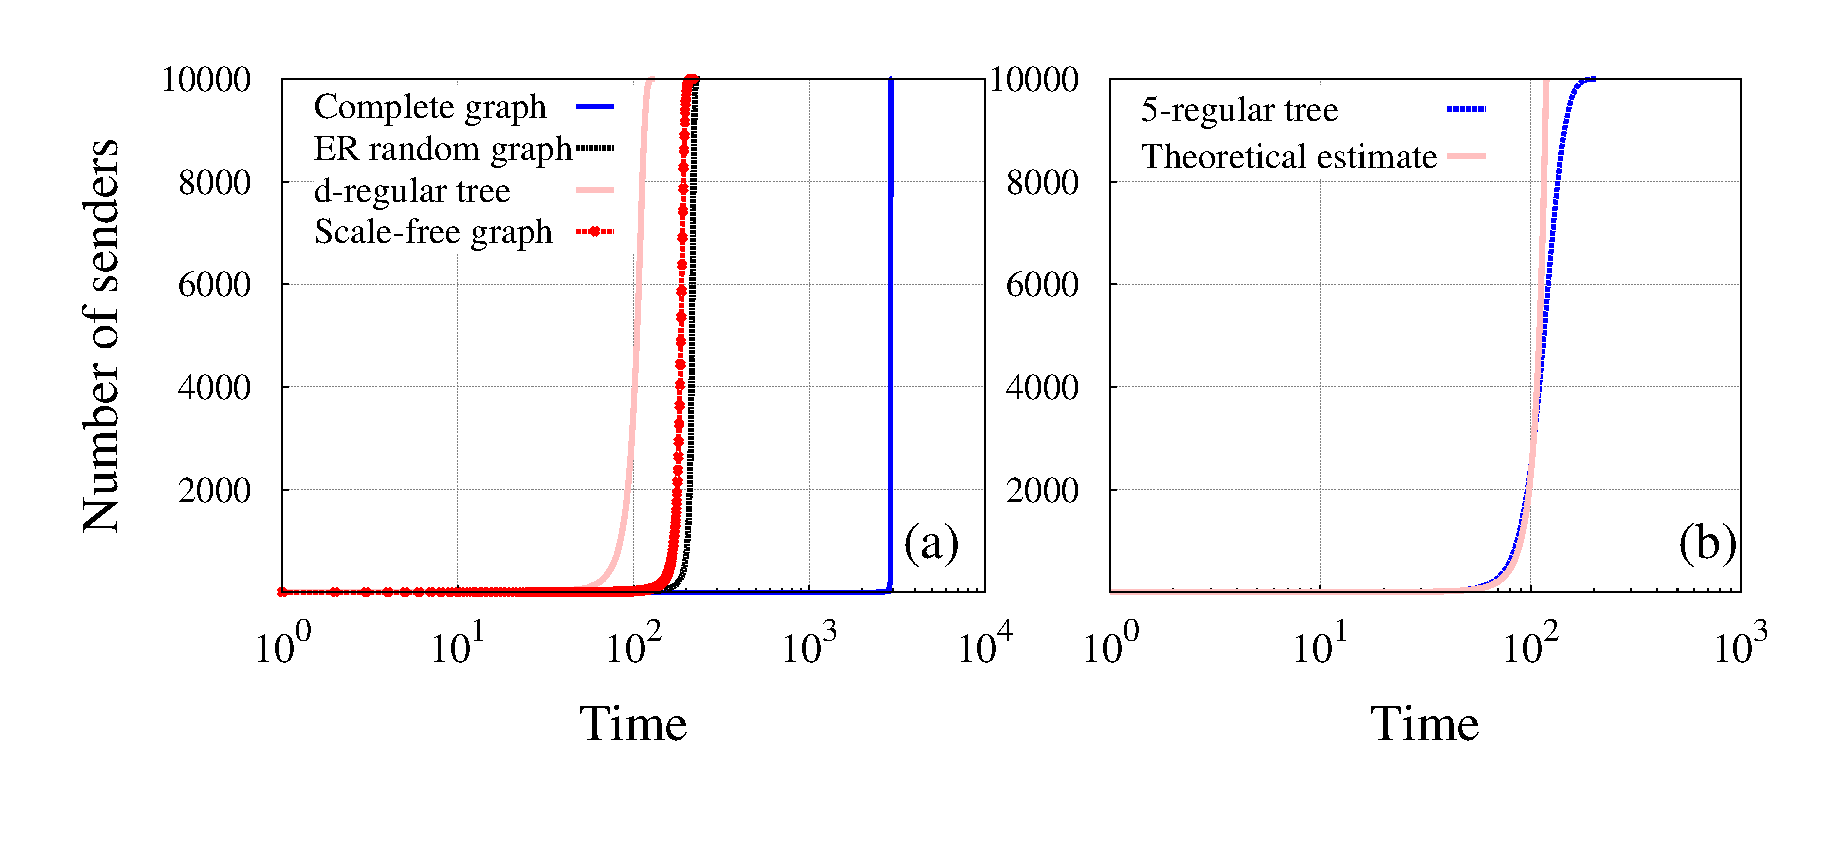
\includegraphics[scale=0.38]{./texfiles/Chapter_3/epl/figs1/plot_all.eps}
  %\includegraphics*[scale=0.28]{figs1/plot_var_k.eps}
 %\includegraphics*[scale=0.15]{figs/T1_vs_exp_T1_d_reg.eps}
 
%\hspace{5mm}(a)\hspace{75mm}(b) 
%\vspace{-4mm}
 \caption{\label{fig1} (a) The number of senders versus time steps for different network topologies (For ER random graph $p$ is $0.005$, for $d$-regular graph $d=5$ and for BA scale-free graph $m$ i.e., number of edges to attach from a new node to existing nodes is $5$) and 
 (b) The theoretical estimate and the simulated result for $d-$regular trees. The theoretical eastimate is obtained from equation 17.}
 \vspace{.5cm}
\end{figure}
 
% \todo{In figure~\ref{fig1} caption, add the vlaue of $p$ for ER graph and $\lambda$ for the scale-free graphs.}
 
Formally, we consider a network topology $G$ = $(V,E)$ where $V$ represents the set of
nodes in the network and $E$ denotes the set of edges between any pair of nodes in $%
V $. We initially start with a single infected node in the system. We
further assume that for a susceptible node to get infected,  $k$ encounters
with infected nodes are required. To put it in a simple way we consider that
a message $M$ needs to be spread over a network and message $M$ consists of $%
k$  identical tokens. At each communication instance one token gets transmitted from an
infected node to the susceptible node. Therefore, number of tokens ($k$) in a
message corresponds to the number of contacts required for a susceptible
node to get infected. Note that for the rest of this chapter we will present
our diffusion model in terms of messages and tokens. 
%Since the infected nodes essentially pass on the tokens we term them as senders while the susceptible ones are the non-senders.  

We assume that at time $0$, there is only one sender (infected) node present in the
system and it acts as the {\em initiator} of the diffusion process. At each
discrete time step a sender node randomly selects one of
its neighbors and  there is a transfer of a token from the sender to the non-sender. A non-sender node becomes a sender only after it receives exactly $k$
tokens (refer to figure \ref{fig_dynamics}). 
The analytical
estimation of the diffusion time based on the underlying topology requires a
case-by-case examination.
We formulate both analytical and empirical results for two extreme variants (in terms of edge density) of networks (a) complete graphs (dense) and (b) infinite regular trees (sparse)
while for others we provide empirical
results with intuitive justifications.
%\todo{Can we have a small picture demonstrating the dynamics since this is a very novel concept? We can take a small network, $k=3$ and illustrate the spread in three time points -- $t=0$ where only one node is black (the initiator), some intermediate $t=t^{'}$ where we show the $k$ values for different nodes (none of which is yet $=3$) and then $t=t^{''}$ where the first sender is formed (one node has $k=3$). We have enough white spaces between figures which can be reduced to fit in this picture.}
\if{0}
%Note that this results in creation of a subgraph at each time step roughly resembling a temporal network. 
% Assuming such a diffusion model we study in detail the diffusion time (i.e.,
% the time from the start till the time when all the nodes in the network
% receive the information and the algorithm terminates) given an underlying
% network topology.
\fi
% \begin{figure}[htpb]
%   \centering
%   \includegraphics[scale=0.28]{figs1/plot_var_k.eps}
%   %\includegraphics*[scale=0.28]{figs1/plot_var_k.eps}
%  %\includegraphics*[scale=0.15]{figs/T1_vs_exp_T1_d_reg.eps}
%  
% %\hspace{5mm}(a)\hspace{75mm}(b) 
%  \caption{\label{fig_k} Number of nodes at each stage of infection versus time for complete graph \todo{write more detailed description}}
% \end{figure}


\if{0} 
% \subsection{Agent configuration and network setup}
% 
% We consider a network topology $G = < V,E >$ where each node in $V$ represents an agent of the network and any link in $E$ represents a contact 
% opportunity between a pair of nodes (agents) in the whole time span through which the network is active. So for any node (agent) $n_{i}$ in this network, its one hop 
% neighbors are the nodes (agents) which are within the connection proximity of $n_{i}$ and at each time step $n_{i}$ at random can connect to any one of them. 
% 
% 
% \subsection{Information configuration}
% 
% As we stated earlier, we consider that the information diffusion occurs in parts. 
% We consider that thdie whole information $\mathcal{M}$ is divided into a set of $m$ tokens, i.e., $|\mathcal{M}| = m$ and in 
% a contact opportunity a single token gets transmitted.
%  We can also extend it to knowledge diffusion or special cases of disease spreading where a susceptible node gets infected 
%  only after it meets infected individuals for specified number of times. In these cases the total number of tokens 
%  would refer to the number of times ($m$) a susceptible (novice) individual communicates with an infected (knowledgeable) individual 
%  before it itself gets infected (knowledgeable). It can further be interpreted as the number of times a node should be reminded of an 
%  information before it remembers and participates in the diffusion process. Note that throughout our analysis we will stick to the 
%  notion of information and tokens for simplicity. 
% 
% 
% \subsection{Information diffusion technique}
% 
% In this framework, transfer of a message during a contact refers to the transfer of one single token of the information. 
% Transfer of a token from $u_i$ to $v_j$ during a contact can take place only 
% when $u_i$ qualifies as a {\em sender} by having all the tokens of the information.
% We mainly consider the $push$ technique of information diffusion which is described below. 
% 
% 
%  \noindent \emph{Push technique:} 
%   \begin{itemize}
%  % \vspace{-3mm}
%    \item \emph{Step 1:} At any time step, $u_i$ (already a sender) establishes a communication link with $v_j$, 
%    from its neighborhood and finds an exclusive set of tokens that $u_i$ has but $v_j$ does not have in its buffer. 
%    \item \emph{Step 2:} If $u_i$ can find such a (non-empty) set, then it transfers only one token from this set to $v_j$. 
%   \end{itemize}
% 
% Next we describe the information diffusion technique which we call $Blind Push$ (B-P) in detail.
% An initiator node is the one which has the full information in the beginning. At each time step all the nodes 
% in the system having the full information communicate with a node in their proximity and try to $push$. 
% %If it is successful then a unit bandwidth is consumed otherwise it is counted as wastage. 
% At the end of each time step all the nodes which have received all the tokens qualify as sender in the next time step. The algorithm terminates 
% when all the nodes in the system have the full information.
% We consider two types of epidemic processes - a) Susceptible-Infected (SI) and b) Susceptible-Infected-Recovered (SIR). 
% Susceptible nodes are the ones having a subset ($S$) of all the tokens ($0\leq |S| < m$, partial information) and the infected nodes are the one with 
% all the tokens (full information). The recovered nodes are the ones, which after having received the full information and spreading it for some time 
% have moved out of the system and is no longer part of the network.
% The information diffusion technique is similar for both the process. 

% \begin{algorithm}
% \caption{Blind Push (B-P)}\label{bp}
% \begin{algorithmic}[1]
% %\Procedure{MyProcedure}{}
% \STATE $select \, initiator$
% \STATE $make \, it \, sender$
% %\BState \emph{top}:
% %\If {$i > \textit{stringlen}$} \Return false
% %\EndIf
% %\State $j \gets \textit{patlen}$
%  \WHILE {$( not \, all \, nodes \, in \, the \, network \, have \, the \, message )$}
%  \FOR {$(each \, node \, which \, is \, already \, a \, sender)$}
% \STATE $select \, a \, node \, from \, its \, proximity;$
% \STATE $perform \, Push$;
% \IF {$(Push \, unsuccessful)$}
% \STATE $wastage;$
% \ELSE 
% \STATE $unit \, bandwidth \, consumed;$
% %\State $i \gets i-1$.
% %\State \textbf{goto} \emph{loop}.
% %\State \textbf{close};
% \ENDIF
% \ENDFOR
% \STATE $modify \, the \, list \, of \, senders;$
% \STATE $increment \, time;$
% \ENDWHILE
% %\EndProcedure
% \end{algorithmic}
% \end{algorithm}

% \subsection{Metrics of interest}
% %\vspace{-2mm}
% We are interested in evaluating the spreading model in terms of the following metrics-
% \begin{itemize}
% %\vspace{-4mm}
%  \item \textbf{Diffusion time $T^*$} - this is the time from the point when the message source starts the diffusion process to the point when all the agents in the network have received the the total information. 
%  $E(T^*)$ denotes the expected diffusion time. In addition, we are also interested in the time $T_i$ which is the minimum time at which there are $i$ senders (except the source) in the network, and especially in $T_1$ since, as we shall see, that this is the prime determinant of the entire broadcast time. 
% %\todo{why are these lines needed - Finally, note that $T^*$ may not correspond to $T_{n-1}$, i.e., the time when there are $n-1$ senders (except the source) in the network because all $n-1$ agents need not become senders to spread the message.}  
%  \item \textbf{Diffusion threshold} - 
% \end{itemize}
% \subsection{Dynamic topology}
% %\vspace{-2mm}
% We performed our experiments on synthetic topologies like complete graph, regular tree, regular graph and random graph. 
% A topology specifies the potential neighborhood of a node 
% - a node at each time step connects randomly to one of these nodes. A complete graph 
% topology would indicate that the 
% node can connect to any other node in the network while for other sparser topology it would 
% connect only to a subset of them.

\medskip
\fi



\noindent
\section{On complete graph}
\label{res_complete}
\noindent For {\bf complete graph} we assume the
number of nodes in the system to be $n$. 
%The time elapsed before the first sender (apart from the initiator) is created is represented by $t_1$ and the total diffusion time is denoted by $T^*$. We denote the expected values of these quantities by $% \mathbb{E}(t_1)$ and $\mathbb{E}(T^*)$ respectively. 
To determine how the number of
senders in the system changes with time, we plot the number of senders
against time for complete graph in figure~\ref{chapter_5_fig1}. 
%We further show in ~\ref{fig_k} how the diffusion progresses by plotting the number of nodes at each stage of infection at every time step for complete graph topology which roughly resembles epidemic process on a heterogenous population.  %Note
%that we assume the $d$-regular tree to be truncated with all the nodes except the leaf
%nodes have degree $d$.
We observe that the diffusion is initially slow which is then followed by a ramp-up after which the diffusion rate becomes almost exponentially fast.
To better analyze the process we divide the process into two phases i) the initial phase and ii) the residual phase. 


\noindent{\bf Initial phase:}  In the spreading process we define the initial phase to be the time between the
initiation and the point at which the first sender is created. We
define this as $t_1$; we will show later that $\hat E(t_1)$ (expected value of $t_1$) is
indeed an indicator for $\hat E(T^*)$ ($T^*$ - 
total diffusion time) in case of a complete graph.

Note that analytically deriving  $\hat E(t_1)$ assuming a  discrete 
(i.e., for a node the delay between two successive contacts is $1$ unit) diffusion model becomes severely complex and hence we adopt a continuous 
variant of the model. In fact, the calculation of the $\Pr \{ t_{1}=t\}$ can be treated as an expected time of filling the first urn with $k$
balls in the experiment where we have initially $d$ empty urns (degree of the node, for complete graph $d \sim n$) and at each
single time step we add a single ball to one urn chosen randomly. 
 For any $k$%
-parts message, by~\cite{kaplan1977generalization} we describe our problem
as a unit-time Poisson process. Note that for a Poisson process the inter-arrival time follows exponential distribution ($\lambda$) and expected number of arrivals in time $t$ is $\lambda t$.  
 Let 
$X_{j}(t)$ be a random value describing the number of balls in $j^\textrm{th}$ urn up
to time $t$. More precisely $X_{j}(t)=\sum_{i=1}^{N}1$ where $N$ is a random variable 
with Poisson distribution $\mathcal{P}(\frac{t}{d})$. Essentially $N$ represents number of draws
of the $j^\textrm{th}$ urn up to time $t$ if $d$ urns exist in the system.
Hence $\{X_{j}(t)\}$s are i.i.ds and $X_{j}(t)\sim\mathcal{P}(\frac{t}{d}%
) $.  
{We formulate the analytical result for complete graph topology through the following theorems 1-5. The various notations are further 
summarized in table \ref{tab:1}}



\begin{theorem}
%\vspace{-.2cm}
For a message with $k$ tokens, the expected value of $t_1$, 
$\hat E(t_{1})=\int_{0}^{\infty}(1-P(t_{1}\leq
t))dt = \int_{0}^{\infty}Q(k,\frac{t}
{d})^{d}dt$
where $Q(k,u)$ is a regularized incomplete gamma function and $d$ is the degree. 
% Furthermore for fixed $i\geq 2$ the random variable $t_{i}d^{-\frac{k-1}{k}}$ converges to a limiting random variable $\tau _{i}$ and the following recursion holds for the expectations: $\frac{\mathbb{E}\left( \tau _{i}\right) }{\mathbb{E}\left( \tau _{i-1}\right) }%=1-\frac{2k-1}{ik} .$
\label{theorem-0}
\end{theorem}

\begin{proof}
 \begin{equation}
\begin{aligned} 
\hat E(t_{1})=&\int_{0}^{\infty}(1-P(t_{1}\leq
t)dt=\int_{0}^{\infty}(1-(1-P(t_{1}
>t))dt\\=&\int_{0}^{\infty}P(X_{j}(t)<k)^{d}dt=\int_{0}^{\infty}Q(k,\frac{t}
{d})^{d}dt\label{eqint} 
\end{aligned}
\end{equation}

where $Q(k,u)$ is a regularized incomplete gamma function~\cite{arfken1985incomplete} i.e. 
\begin{equation}
Q(k,u)=\frac{\Gamma(k,u)}{\Gamma(k)}=e^{-u}\sum_{l=0}^{k-1}\frac{u^{l}}{l!}
\end{equation}
is valid for any natural $k$ and non-negative $u$.

\end{proof}

%\vspace{-.2cm}
Note that $t_{1}$ for a Poisson process, is a continuous random variable. 

\noindent{\bf Residual phase:} We next proceed to establish the relation between $\hat E(t_1)$ and $\hat E(T^{*})$. Apart from assuming the continuous model, 
we compute scaled $t_1$ and $T^{*}$ (by $d^{\frac{k-1}{k}}$, 
(this specific scaling function was initially calculated for $k=2$ and then generalized for higher values)) instead of their explicit values to further aid our analysis. 
To summarize, we start by computing  
expected values of scaled $t_1$ and $T^{*}$ considering a continuous (Poisson) model with $d\rightarrow \infty$ and show that the results hold for finite $d$. Finally, we show that the results for the continuous model extend to the discrete model.
We begin by showing that $t_1$ (time to create the first sender apart from the initiator) is an indicator for the diffusion delay $T^*$ through the following two theorems. 
%The detailed proof of both the theorems are available in the supplementary.


\begin{table}
\centering
\caption{Summary of the notations used.}
\label{tab:1}
\scalebox{0.65}{
\begin{tabular}{|l|l|}
\hline
{\bf Symbol}             & {\bf Definition}                                                                     \\ \hline\hline
$t_1$              & Time between initiation and creation of first sender                           \\ \hline
$T^{\ast}$         & Total diffusion time                                                           \\ \hline
$\hat E(t_1)$      & Expected $t_1$ (obtained analytically)                                         \\ \hline
$\hat E(T^{\ast})$ & Expected $T^{\ast}$(obtained analytically)                                     \\ \hline
$Av(t_1)$          & Expected $t_1$ (obtained empirically)                                          \\ \hline
$Av(T^{\ast})$     & Expected $T^{\ast}$ (obtained empirically)                                     \\ \hline
$s_1$              & Limiting random variable of $t_{1}d^{- \frac{k-1}{k}}$as $d\rightarrow \infty$ \\ \hline
$\tau_i$           & Scaled time span between creation of $(i-1)^{th}$ sender and $i^{th}$ sender   \\ \hline
$s^{\ast}$         & Limiting random variable for $T^{\ast}d^{-\frac{k-1}{k}}$                      \\ \hline
\end{tabular}}
\end{table}

\begin{theorem}
%\vspace{-.2cm}
For a message with $k$ tokens the random variable $t_{1}d^{-\frac{k-1}{k}}$
converges as $d\rightarrow \infty $ to a limiting random variable $s_{1}$
with density $\frac{x^{k-1}}{(k-1)!}e^{-\frac{x^{k}}{k!}}$ 
and expectation $%
\hat E \left( s_{1}\right) =(k!)^{\frac{1}{k}}\Gamma\left(1+\frac{1}{k%
}\right).$ 
% Furthermore for fixed $i\geq 2$ the random variable $t_{i}d^{-\frac{k-1}{k}}$ converges to a limiting random variable $\tau _{i}$ and the following recursion holds for the expectations: $\frac{\mathbb{E}\left( \tau _{i}\right) }{\mathbb{E}\left( \tau _{i-1}\right) }%=1-\frac{2k-1}{ik} .$
\label{theorem-1}
\end{theorem}
%\vspace{-.2cm}

\begin{proof}
 The proof is based on Poisson clock approximation approach
introduced {previously.} 
% which means that variables are
% independent and for a price of acceptable level of error of the order $%
% o_d(1) $. 
We start from the calculation of the CDF for the random variable $%
t_1 d^{-\frac{k-1}{k}}$:


\begin{equation}
\begin{aligned} &F_{t_1 d^{-\frac{k-1}{k}}}(x)=P(t_1 d^{-\frac{k-1}{k}}\leq
x)\\
%=1-P(t_1>xd^{\frac{k-1}{k}})\\
%&=1-P(X_j(xd^{\frac{k-1}{k}})<k)^d
&=1-Q(k,\frac{xd^{\frac{k-1}{k}}}{d})^d%
\\
&=1-\left(\sum_{i=0}^{k-1}e^{-xd^{-\frac{1}{k}}}(xd^{-%
\frac{1}{k}})^i/i!\right)^d\\ \label{eq-prof-1}
%&=1-\left(1-e^{-xd^{-\frac{1}{k}}}(xd^{-%
%\frac{1}{k}})^k/k!(1+o(1))\right)^d 
 \end{aligned}
\end{equation}

where in the last line we used the common simple approximation of Poisson
cumulative distribution in long tail.

Since we are interested in limits as $d\rightarrow \infty$, for $%
exp(-xd^{-\frac{1}{k}})\rightarrow 1$ and we can compute limits of $F_{t_1
d^{-\frac{k-1}{k}}}$ 
as follows: 
\begin{equation}
\begin{aligned} F_{s_1}(x)&=\lim_{d\rightarrow\infty}F_{t_1
d^{-\frac{k-1}{k}}}(x)\\&=\lim_{d\rightarrow\infty}1-\left(\sum_{i=0}^{k-1}e^{-xd^{-\frac{1}{k}}}(xd^{-%
\frac{1}{k}})^i/i!\right)^d \\&=
1-e^{(-x^k/k!)} \label{eq-prof-cdf1} \end{aligned}
\end{equation}

Now, the density function of $\tau_1$ can be calculated as - 

\begin{equation}
f_{s_1}(x)=\frac{dF_{s_1}}{dx}(x)=\frac{x^{k-1}}{(k-1)!}exp%
\left(-\frac{x^{k}}{k!}\right)
\end{equation}
Further the expectation of $s_{1}$ is - 
 \begin{equation}
\begin{aligned}
\hat E(s_1)&=\int_{0}^{\infty}xf_{s_1}(x)dx=\int_{0}^{\infty}%
\left(uk!\right)^{\frac{1}{k}}e^{-u}du\\&=\left(k!\right)^{\frac{1}{k}}%
\int_{0}^{\infty}u^{\frac{1}{k}}e^{-u}du=\left(k!\right)^{\frac{1}{k}}\Gamma%
\left(1+\frac{1}{k}\right) \label{e-tau-1} 
\end{aligned}
\end{equation}
\end{proof}



We next compute the expectation of the (scaled) time $%
T^{\ast }$ till all nodes become senders.  
We consider $T_{i}=t_{i}d^{-\frac{k-1}{k}}$. We further assume $\tau _{i}$ as the
scaled time span between the creation of $(i-1)^\textrm{th}$ new sender and that of $i^\textrm{th}$ new
sender. Correspondingly $\tau _{i}^{\ast }$ represents the scaled time for
the original process where every node with at least $k$ tokens acts as a
sender node.  
We have $\hat E\left( \tau _{i}^{\ast }\right) =%
\frac{1}{i}\hat E\left( \tau _{i}\right) =\frac{1}{i}\left( \hat E%
\left( T_{i}\right) -\hat E\left( T_{i-1}\right) \right)$.  
Note that $\tau _{1}$ is equal to $T_{1}$ as $T_{0}$ is 0 and hence $\hat E(s_1)$ equals $\hat E(\tau _1)$.
%\vspace{-.2cm}
\begin{theorem}
%\vspace{-.2cm}
\label{theorem-2} $T^{\ast }d^{-\frac{k-1}{k}}$ converges to a limiting
random variable $s^{\ast }$ with 
%\vspace{-.2cm}
\begin{equation*}
\vspace{-.3cm}
\hat E \left( s^{\ast }\right) =\sum\limits_{i=1}^{\infty }\hat E%
\left( \tau _{i}^{\ast}\right) = \hat E(\tau_1)\frac{k}{k-1}
\end{equation*}
\end{theorem}

\begin{proof}
$G_{i}^{\left( d\right) }\left( z\right)
=1-F_{i}^{\left( d\right) }\left( z\right) =\Pr \left\{ t_{i}>zd^{\frac{k-1}{%
k}}\right\} =\Pr \left\{ T_{i}>z\right\} $ (complementary cdf of $T_i$). Since $\frac{zd^{\frac{k-1}{k}}}{%
d}=zd^{-\frac{1}{k}}$ we have 
\begin{equation}
\begin{aligned} G_{i}^{\left( d\right) }\left( z\right)
=&\sum_{j=0}^{i-1}\binom{d}{j}\left( \sum_{l=0}^{k-1}\frac{1}{l!}\left(
zd^{-\frac{1}{k}}\right) ^{l}e^{-zd^{-\frac{1}{k}}} \right)
^{d-j}\\&\left( 1-\sum_{l=0}^{k-1}\frac{1}{l!}\left(
zd^{-\frac{1}{k}}\right) ^{l}e^{-zd^{-\frac{1}{k}}} \right)
^{j} \\
%=&\sum_{j=0}^{i-1}\binom{d}{j}\left( 1-\left( 1+o_{d}\left( 1\right)
%\right) \frac{z^{k}d^{-1}}{k!}e^{-zd^{\frac{-1}{k}}}\right) ^{d-j}\\&\left(
%\left( 1+o_{d}\left( 1\right) \right)
%\frac{z^{k}d^{-1}}{k!}e^{-zd^{\frac{-1}{k}}}\right) ^{j} \\
%=&\sum_{j=0}^{i-1}\frac{d^{j}}{j!}\left( \frac{z^{k}}{k!}\right)
%^{j}\frac{1}{d^{j}}e^{-\frac{z^{k}}{k!}}\left( 1+o_{d}\left( 1\right)
%\right) \\
=&\sum_{j=0}^{i-1}\frac{1}{j!}\left( \frac{z^{k}}{k!}\right)
^{j}e^{-\frac{z^{k}}{k!}}\left( 1+o_{d}\left( 1\right) \right) 
\end{aligned}
\end{equation}
taking limits $d\rightarrow \infty $ and using the abbreviation $a=\frac{%
z^{k}}{k!}$ we obtain for $G_{i}\left( z\right) =\lim_{d\rightarrow \infty
}G_{i}^{\left( d\right) }$ and
%=1-F_{i}\left( z\right) $ the expression%
%\todo{I dont see any usage of $F_i$ so why mentioning it in a equation (9). - remove eq. 9}
\begin{eqnarray}
G_{i}\left( z\right) &=&\sum_{j=0}^{i-1}\frac{a^{j}}{j!}e^{-a} 
\end{eqnarray}
%F_{i}\left( z\right) &=&1-\sum_{j=0}^{i-1}\frac{a^{j}}{j!}e^{-a}.
%
Subsequently,  we get for $\hat E \left( \tau _{i}\right) =\int \left(
G_{i}\left( z\right) -G_{i-1}\left( z\right) \right) dz:$%
\begin{eqnarray}
\hat E \left( \tau _{i}\right) &=&\int_{0}^{\infty }\frac{1}{\left(
i-1\right) !}\left( \frac{z^{k}}{k!}\right) ^{i-1}e^{-\frac{z^{k}}{k!}}dz ,
\\
\hat E \left( \tau _{i}^{\ast }\right) &=&\int_{0}^{\infty }\frac{1}{i}%
\frac{1}{\left( i-1\right) !}\left( \frac{z^{k}}{k!}\right) ^{i-1}e^{-\frac{%
z^{k}}{k!}}dz .
\end{eqnarray}%
For computing $\mathop{\displaystyle \sum }\limits_{i=1}^{N}\hat E\left(
\tau _{i}^{\ast }\right) $ we can exchange integration and summation. Hence
we first estimate 
\begin{equation}
\begin{aligned} \lim_{N\rightarrow \infty }\mathop{\displaystyle \sum
}\limits_{i=1}^{N}\frac{1}{ i !}a^{\left( i-1\right) }e^{-a}
&=&\frac{1}{a}\left(
1-e^{-a}\right)
%&\lim_{N\rightarrow \infty }\frac{1}{a}\mathop{\displaystyle \sum
%}\limits_{i=0}^{N}\frac{1}{(i+1)!}a^{i+1}e^{-a} \\ 
%&=&\frac{1}{a}\left(
%1-e^{-a}\right). 
\end{aligned}
\end{equation}

Transforming variables in the integral as $y=\frac{z^{k}}{k!}$ we
finally get 
\begin{equation}
\hat E \left( s^{\ast }\right) =\frac{\left( k!\right) ^{\frac{1}{k}}}{k-1%
}\Gamma \left( \frac{1}{k}\right)= \hat E(\tau_1)\frac{k}{k-1}
\end{equation}

\end{proof}

We observe from the above result that the expectation of scaled $T^{*}$ converges to a value which depends only on $k$ which is constant for a given setting. 
Hence we conclude that the expectation of {\bf $T^{*}$ is proportional to $d^{\frac{k-1}{k}}$} and similarly for $t_1$.

The above results are based on the assumption that $i$ is fixed as  
%as I understand the number of sender would also increase exponentially - then does the limit hold}) is fixed and $%
$d\rightarrow \infty .$  
We now proceed to show that the computations hold for finite $d$ for $i$ varying with $d$.
Note that the above formulae hold true for $i\leq f\left( d\right) $ as
long as $f\left( d\right) =o\left( d^{\frac{1}{k}}\right) .$ 


\begin{theorem}
%\vspace{-.2cm}
\label{theorem-3}
Considering that the range of $i$ (number of senders) varies with $d$ (degree) if $f\left( d\right) =d^{\frac{1}{k}-\epsilon }$
for some $\epsilon >0$, %
$\sum_{i>f\left( d\right) }^{d}\tau _{i}^{\ast }\left( d\right) =o_{d}\left(
\sum_{i\geq 1}^{f\left( d\right) }\tau _{i}^{\ast }\left( d\right) \right) $
\end{theorem}
%\vspace{-.2cm}

\begin{proof}
We compute first $\mathbb{E}\left( \tau _{i}\right)
=\int_{0}^{\infty }\frac{1}{\left( i-1\right) !}\left( \frac{z^{k}}{k!}%
\right) ^{i-1}e^{-\frac{z^{k}}{k!}}dz$ using again the transformation of
variables $y=\frac{z^{k}}{k!}$

\begin{eqnarray}
\hat E \left( \tau _{i}\right) &=&\frac{1}{\left( i-1\right) !}\frac{\left( k!\right) ^{1/k}}{%
k}\int_{0}^{\infty }y^{i-2+\frac{1}{k}}e^{-y}dy \\
&=&\frac{1}{\left( i-1\right) !}\frac{\left( k!\right) ^{1/k}}{k}\Gamma
\left( i-1+1/k\right)
\end{eqnarray}

%.

%\todo{Lets discuss this part}

%For large $i$ we have by Stirlings formula $\Gamma \left( i-1+1/k\right)
%\simeq \sqrt{2\pi }\frac{\left( i-2+1/k\right) ^{i-3/2+1/k}}{e^{i-2+1/k}}$
%and
Using Stirling's approximation~\cite{feller2008introduction} we obtain - \\
%$\left( i-1\right) !\simeq \sqrt{2\pi \left( i-1\right) }\left( \frac{i-1%
%}{e}\right) ^{i-1}$ hence 
\begin{equation}
\frac{\Gamma \left( i-1+1/k\right) }{\left( i-1\right) !}\simeq e^{-2+\frac{2%
}{k}}\frac{1}{\left( i-1\right) ^{1-1/k}}
\end{equation}
The further argumentation is independent of the involved constant
coefficients since we only need leading orders.

We have -  
\begin{equation}
\begin{aligned} T_{L}&=\sum_{1}^{L}\hat E \left( \tau _{i}\right)
=O\left( 1\right) \cdot \sum_{1}^{L}\frac{\Gamma \left( i-1+1/k\right)
}{\left( i-1\right) !}\\&=O\left( 1\right)
\int_{1}^{L}\frac{1}{x^{1-1/k}}dx= O\left( 1\right) L^{1/k}. \end{aligned}
\end{equation}

Note once more that all the computations up to now are in scaled time units.
Hence in real time we have $t_{L}\sim $ $L^{1/k}d^{1-\frac{1}{k}}.$ Setting $%
L\sim d^{\frac{1}{k}-\epsilon }$ we get $t_{L}=d^{1-\frac{1}{k}+1/k^{2}-%
\frac{\epsilon }{k}}.$ Taking $t_{L}$ as unit and taking into account that
the total time  $t^{\ast
}=\left( 1+o\left( 1\right) \right) d\log d$ (in the scaled process), we have according to the
results in \cite{kaplan1977generalization}, $t^{\ast }=$ $O\left(
1\right) \cdot t_{L}\cdot d^{\frac{1}{k}-1/k^{2}+\frac{\epsilon }{k}}\log d.$
But since the acceleration at this point is $d^{1/k-\epsilon }$ we have for
the remaining time (that is the time after the $d^{\frac{1}{k}-\epsilon }$%
-th event) in the accelerated process a contribution of at most $\tilde{t}%
_{L}d^{-1/k^{2}+\frac{\epsilon }{k}+\epsilon }\cdot \log d=\tilde{t}%
_{L}\cdot o_{d}\left( 1\right) $ since $\epsilon $ can be chosen arbitrary
small - here $\tilde{t}_{L}$ denotes the time till the $L^\textrm{th}$ event in the
accelerated process. This shows that $\sum_{i>f\left( d\right) }^{d}\tau
_{i}^{\ast }\left( d\right) =o_{d}\left( \sum_{i\geq 1}^{f\left( d\right)
}\tau _{i}^{\ast }\left( d\right) \right) .$

\end{proof}

{The above results show that previous computations (considering $d\rightarrow \infty$) give correct limiting values. 
This indicates that our analysis is able to correctly estimate the diffusion time for a complete graph of finite size.}


It now remains to show that the asymptotic estimations for the model with
Poisson clock carry over to the discrete time model (which we use for our simulations) defined at the
beginning. Note that the discrete time model is actually the Poisson
model when looked at in event time steps, where events here are the
times when a token is sent. 
%Consider first the time $t_{i}$ that is the
%real time between the creation of $(i-1)$$^\textrm{th}$ and $i$$^\textrm{th}$ sender in the Poisson model. 

\begin{theorem}
%\vspace{-.2cm}
 If $t_{i}$ is the time between the creation of the $(i-1)^\textrm{th}$ and $i^\textrm{th}$ sender and 
 $\hat{t}_{i}$ is the corresponding time in the discrete model, then $\hat E \left( \hat{t}_{i}\right) =\hat E \left( t_{i}\right)
\left( 1+o_{d}\left( 1\right) \right) $ 
\end{theorem}
%\vspace{-.2cm}
%\todo{Is the proof starting here?}
\begin{proof}
Since we have $i$ independent senders all acting with Poisson clocks of
intensity $1$ we have the time between two tokens sent - denoted in the
following by a random variable $x$ - to be an exponential distribution $%
Exp\left( i\right).$ We index the events by $l$ and observe that $t_{i}=%
\sum\limits_{l=1}^{K_{i}}x_{l}$ where $K_{i}$ is the
random stop time when the $i^\textrm{th}$ sender is created. In the discrete model $i$
messages are sent simultaneously 
hence $i$ successive events in the Poisson
model correspond to one time step in the discrete model. Hence $\hat{t}%
_{i}=\left\lfloor \frac{1}{i}\cdot K_{i}\right\rfloor =\frac{1}{i}\cdot
K_{i}\cdot \left( 1+o_{d}\left( 1\right) \right) $ . Since the $\left\{
x_{l}\right\} $s are i.i.ds we can apply Wald's theorem \cite{wald} and get 
\begin{center}
$\hat{E}\left( t_{i}\right) =\hat{E}\left( K_{i}\right) \hat{E}%
\left( x\right) =\frac{1}{i}\hat{E}\left( K_{i}\right)$ 
\end{center}%
hence $\hat{E}\left( \hat{t}_{i}\right) =\hat{E}\left( t_{i}\right)
\left( 1+o_{d}\left( 1\right) \right) $ and the analytical results for the poisson model hold for the discrete case as well.
\end{proof}

We further simulate our diffusion model on complete graphs to verify our analytical results. 
For this
purpose, we plot in figure \ref{segSizeVsDelay_nrTrans_varyN_Mall_push_pull}
the values of {average diffusion time ($Av(T^{\ast })$)} and {average time to create the first sender ($Av(t_{1})$)} respectively as we vary the size of the network. We further 
report the values of $Av(T^{\ast })$ and $Av(t_{1})$ for different values of $k$
with network size fixed at $1000$. 
Note that
the two quantities $Av(T^{\ast })$ and $Av(t_{1})$ (the results were averaged over $1000$ simulations) exhibit a
very similar profile irrespective of the chosen value of $k$. 
In the same
figure we also plot the function 
 $d^{\frac{k-1}{k}}$ (represented by $\hat E(t_1)$) { obtained from theorem \ref{theorem-1}}, suitably scaled by a
constant to show how the theoretical results closely follow  the
numerical simulations.

 \begin{figure}[htbp] 
 %\vspace{-.3cm}
 \centering
 \includegraphics[scale=0.4]{./texfiles/Chapter_3/epl/figs1/plot_var_n_k_complete.eps}
 
 %\vspace{-5mm}
 \caption{$Av(T^*)$ and $Av(t_1)$ versus (a) the number of nodes with message size $k=4$ and (b) $k$ for fixed $d=1000$.
  For both the plots $\hat E(t_1) = C \ast d^{\frac{k-1}{k}}$ where $C = (k!)^{\frac{1}{k}}\Gamma\left(1+\frac{1}{k}\right)$ (refer to theorem \ref{theorem-1}).}
 \label{segSizeVsDelay_nrTrans_varyN_Mall_push_pull}
 %\vspace{-.3cm}
 \end{figure}
% The
% remaining growth is very fast - actually of logarithmic order since several
% new senders in every time step get produced. \vspace{-2mm}

%{\bf E-R Random graphs} - 


\noindent{\em E-R random graph}: We further look into {\bf Erdos-Renyi random graphs}~\cite{erdos1959random} and observe that for sufficiently 
dense graphs (i.e., having high edge probability) the analysis on the complete graph case holds.  
In this regard we first plot $Av(T^{\ast})$ (obtained through simulations) and $\hat{E}(T^{\ast})$ ($n^{\frac{k-1}{k}}$ scaled by a constant, $n$ is the number of nodes) for 
different values of $k$ (message size) (refer to figure \ref{fig_diff_g_n_p}(a)). 
Clearly, the theoretical estimate closely follows the simulated result. {As we increase the value of edge probabilities ($p$) (i.e., make the network more dense)
 the closer it gets to the theoretical estimate.}
We further plot $Av(T^{\ast})$ (scaled by $\hat{E}(t_{1})$) for varying $p$ in figure \ref{fig_diff_g_n_p}(b). 
The value gets close to 2 with edge probability 1 but remains close to 2 even for lower values of $p$. 
All the results are averaged over $1000$ simulations.



\begin{figure}[htpb]
%\vspace{-.4cm}
\centering
  \includegraphics[scale=0.4]{./texfiles/Chapter_3/epl/figs1/ER_graph_result.eps}
  
  %\vspace{-3mm}
  \caption{\label{fig_diff_g_n_p}(a) $Av(T^{\ast})$ and $\hat E(T^{\ast})$ (suitably scaled) for different values of $k$ 
  (b)$Av(T^{\ast})$ versus edge probability in Erdos-Renyi random graph for $k=2$ and $k=3$. In both cases $Av(T^{\ast})$ is normalized by $\hat{E}(t_{1})$ which is $\sqrt{n}$ and $n^{\frac{2}{3}}$ for $k=2$ and $k=3$ respectively.
  \vspace{5mm}}
  %\vspace{-.5cm}
 \end{figure}

%  \begin{figure}[htpb]
%  \centering
%   \includegraphics[scale=0.28]{figs1/tree_ratio.eps}
%   \caption{\label{tree_ratio} ratio of $s_t$ and $s_{t-1}$ throughout the 
% whole duration of the diffusion process for a 5-regular tree }
%  \end{figure} 

\medskip


\noindent
\section{On $d$-regular tree:}
\noindent We next consider the case of {\bf $d$-regular trees} for $d\geq 3$ (at least $2$ children apart from $1$ parent) with a
distinguished root index $0$ which acts as the initial sender. For
simplicity we give the root an out-degree of $(d-1)$ by attaching a virtual
``mother vertex'' to the root which is also a sender but has only one
offspring and is not counted in the estimation of sender nodes (this helps
us avoid handling the initial steps (i.e., when only the root is having the
message) differently from the later steps). Let $A_{l}\left( t\right) ,$ $%
0\leq l<k,$ be the number of nodes on the tree which have exactly $l$
packets at time $t$ and have a direct communication link to one of the
sender nodes at time $t$. Note that each of the so defined nodes has exactly
one connection to a sender node due to the tree structure and the initial
condition of having just one sender at the beginning. We get the following
 exact linear recursion for the expectation $a_{l}\left( t+1\right) :=\hat{%
E}\left( A_{l}\left( t+1\right) \right) $ at time $t+1:$%
\begin{eqnarray*}
\nonumber
a_{l}\left( t+1\right) &=&\frac{d-1}{d}a_{l}\left( t\right) +\frac{1}{d}% 
a_{l-1}\left( t\right) ,1\leq l\leq k-1 \\ \nonumber
a_{0}\left( t+1\right) &=&\frac{d-1}{d}a_{k-1}\left( t\right) +\frac{d-1}{d}%
a_{0}\left( t\right) \nonumber
\end{eqnarray*}%
Note that for the expected number of sender nodes $s_{t}$ at time $t$, we
have 
\begin{equation}
s_{t}=\sum\limits_{t^{\prime }<t}\frac{1}{d}a_{k-1}\left( t^{\prime }\right)
\end{equation}

The asymptotic rate of growth of the variables $\left\{ a_{i}\left( t\right)
\right\} $ as well as $s_{t}$ is entirely determined by the value of the
largest eigenvalue of the associated transition matrix. The maximal
eigenvalue of the associated characteristic polynomial is given by 
\begin{equation*}
\lambda _{\max }=\frac{d-1}{d}+\left( \frac{d-1}{d}\left( \frac{1}{d}\right)
^{k-1}\right) ^{\frac{1}{k}}=\frac{d-1+\left( d-1\right) ^{1/k}}{d}
\end{equation*}


% \begin{figure}[htpb]
% %\vspace{-.5cm}
%  \centering
%   \includegraphics[scale=0.31]{figs1/plot_reg_tree.eps}
%   %\vspace{-5mm}
%   \caption{\label{tree_ratio}(a) Rate of diffusion ($s_t$ - $s_{t-1}$) throughout the 
% whole duration of the diffusion process for a 5-regular tree. (b) Number of nodes at each stage of infection versus time for 
% complete graph of $1000$ nodes with $k=4$. Although the creation of infected nodes is slow initially, the number of partially infected nodes ($0<p<4$) increases rapidly. (inset) Magnified version of the same figure.}
% %\vspace{-.45cm}
%  \end{figure} 

{In figure \ref{fig1}(b) we draw the diffusion dynamics for a 5-regular tree and in the same figure we show that the
analytical estimate (obtained from equation 17) of diffusion rate closely resemble the empirical
observation. 
\if{0}
to the point where the first leaf node receives the full message. 
%At this point, the leaf nodes are the only non-sender nodes in the network which can only be infected by the nodes in the previous level.
Since the leaf nodes after getting infected have no other nodes to infect,  the dynamics
slows down as is evident in the  figure  - the impact of finiteness on 
diffusion conspicuously gets illustrated in figure \ref{tree_ratio}(a)) where we look into the difference of $s_t$ and $s_{t-1}$ throughout the 
whole duration of the diffusion process. We observe that the diffusion rate initially follows an increasing trend and then drops.
\fi
%We observe that the ratio quickly stabilizes to $\lambda_{max}$ (represented in the same figure) after initial few time steps hence supporting our theory.  
%This is followed by a drop in diffusion rate as by that time infection reaches the leaf nodes.}
%\todo{Why should $\lambda_{max}$ = 1, it should be near to 2, check carefully.}

%\noindent {\em d-regular graph}: 
%We further observe that our analytical estimate for $d$-regular trees could be extended for {\bf $d$-regular graph} as well. We
%observe that the analytical estimate closely follows the empirical
%observations as is evident from figure \ref{fig1}. 
\begin{figure}[htpb]
%\vspace{-.5cm}
 \centering
  \includegraphics[scale=0.4]{./texfiles/Chapter_3/epl/figs1/plot_reg_tree.eps}
  %\vspace{-5mm}
  \caption{\label{tree_ratio}(a) $\frac{t_{1}^{\hat p} - t_1}{t_1}$ versus $\bar p$ for a complete graph with $1000$ nodes and $k=4$.
  (b) Number of nodes at each stage of infection versus time for 
complete graph of $1000$ nodes with $k=4$. Although the creation of infected nodes is slow initially, the number of partially infected nodes ($0<l<4$) increases rapidly. 
(inset) Magnified version of the same figure.}
\vspace{.45cm}
 \end{figure} 


\medskip


\noindent
\section{Discussion}
\label{discussion}
\medskip




% \acknowledgments
% Marcin Bodych and Tyll Krueger were supported by Indian Institute of Technology Kharagpur, Wroclaw University of Technology and the National Science Centre Poland (NCN) through grant no. 2013/11/B/HS4/01061: Agent based modeling of innovation diffusion.
% 
% \begin{thebibliography}{10}
% \expandafter\ifx\csname url\endcsname\relax\def\url#1{\texttt{#1}}\fi
% 
% \bibitem{anderson1992infectious}
% \Name{Anderson R.~M., May R.~M. \and Anderson B.} \Book{Infectious diseases of
%   humans: dynamics and control} Vol.~28 (Wiley Online Library) 1992.
% 
% \bibitem{watts2002simple}
% \Name{Watts D.~J.} \REVIEW{Proceedings of the National Academy of
%   Sciences}{99}{2002}{5766}.
% 
% \bibitem{dodds2004universal}
% \Name{Dodds P.~S. \and Watts D.~J.} \REVIEW{Physical review
%   letters}{92}{2004}{218701}.
% 
% \bibitem{pnas1}
% \Name{Kramer A.~D., Guillory J.~E. \and Hancock J.~T.} \REVIEW{Proceedings of
%   the National Academy of Sciences}{111}{2014}{8788}.
% 
% \bibitem{pnas2}
% \Name{Aral S., Muchnik L. \and Sundararajan A.} \REVIEW{Proceedings of the
%   National Academy of Sciences}{106}{2009}{21544}.
% 
% \bibitem{tang2009epidemic}
% \Name{Tang M., Liu Z. \and Li B.} \REVIEW{EPL (Europhysics
%   Letters)}{87}{2009}{18005}.
% 
% \bibitem{son2012percolation}
% \Name{Son S.-W., Bizhani G., Christensen C., Grassberger P. \and Paczuski M.}
%   \REVIEW{EPL (Europhysics Letters)}{97}{2012}{16006}.
% 
% \bibitem{takaguchi2013bursty}
% \Name{Takaguchi T., Masuda N. \and Holme P.} \REVIEW{PloS
%   one}{8}{2013}{e68629}.
% 
% \bibitem{karsai2011small}
% \Name{Karsai M., Kivel{\"a} M., Pan R.~K., Kaski K., Kert{\'e}sz J.,
%   Barab{\'a}si A.-L. \and Saram{\"a}ki J.} \REVIEW{Physical Review
%   E}{83}{2011}{025102}.
% 
% \bibitem{karimi2013threshold}
% \Name{Karimi F. \and Holme P.} \REVIEW{Physica A: Statistical Mechanics and its
%   Applications}{392}{2013}{3476}.
% 
% \bibitem{backlund2014effects}
% \Name{Backlund V.-P., Saram{\"a}ki J. \and Pan R.~K.} \REVIEW{Physical Review
%   E}{89}{2014}{062815}.
% 
% \bibitem{rocha2013bursts}
% \Name{Rocha L.~E. \and Blondel V.~D.} \REVIEW{PLoS Comput
%   Biol}{9}{2013}{e1002974}.
% 
% \bibitem{masuda2013predicting}
% \Name{Masuda N. \and Holme P.} \REVIEW{F1000 prime reports}{5}{2013}{6}.
% 
% \bibitem{prl1}
% \Name{Bogu{\~n}{\'a} M., Castellano C. \and Pastor-Satorras R.}
%   \REVIEW{Physical review letters}{111}{2013}{068701}.
% 
% \bibitem{van2012epidemic}
% \Name{Van~Mieghem P.} \REVIEW{EPL (Europhysics Letters)}{97}{2012}{48004}.
% 
% \bibitem{zhang2014susceptible}
% \Name{Zhang Y.-Q. \and Li X.} \REVIEW{EPL (Europhysics
%   Letters)}{108}{2014}{28006}.
% 
% \bibitem{joh2009dynamics}
% \Name{Joh R.~I., Wang H., Weiss H. \and Weitz J.~S.} \REVIEW{Bulletin of
%   mathematical biology}{71}{2009}{845}.
% 
% \bibitem{sanghavi2007gossiping}
% \Name{Sanghavi S., Hajek B. \and Massouli{\'e} L.} \REVIEW{IEEE Transactions on
%   Information Theory}{53}{2007}{4640}.
% 
% \bibitem{qiu2004modeling}
% \Name{Qiu D. \and Srikant R.} \Book{Modeling and performance analysis of
%   bittorrent-like peer-to-peer networks} in proc. of \Book{ACM SIGCOMM computer
%   communication review} Vol.~34 (ACM) 2004 pp. 367--378.
% 
% \bibitem{romero2011differences}
% \Name{Romero D.~M., Meeder B. \and Kleinberg J.} \Book{Differences in the
%   mechanics of information diffusion across topics: idioms, political hashtags,
%   and complex contagion on twitter} in proc. of \Book{Proceedings of the 20th
%   international conference on World wide web} (ACM) 2011 pp. 695--704.
% 
% \bibitem{granovetter1978threshold}
% \Name{Granovetter M.} \REVIEW{American journal of sociology}{}{1978}{1420}.
% 
% \bibitem{sur1}
% \Name{Mollison D.} \Book{Epidemic models: their structure and relation to data}
%   Vol.~5 (Cambridge University Press) 1995.
% 
% \bibitem{volz2007susceptible}
% \Name{Volz E. \and Meyers L.~A.} \REVIEW{Proceedings of the Royal Society of
%   London B: Biological Sciences}{274}{2007}{2925}.
% 
% \bibitem{kaplan1977generalization}
% \Name{Kaplan N.} \REVIEW{Journal of Applied Probability}{}{1977}{212}.
% 
% \bibitem{wald}
% \Name{Wald A.} \REVIEW{The Annals of Mathematical Statistics}{15}{1944}{283}.
% 
% \bibitem{erdos1959random}
% \Name{Erd{\"o}s P. \and R{\'e}nyi A.} \REVIEW{Publicationes Mathematicae
%   (Debrecen)}{6}{1959}{290}.
% 
% \bibitem{barabasi1999emergence}
% \Name{Barab{\'a}si A.-L. \and Albert R.} \REVIEW{science}{286}{1999}{509}.
% 
% \end{thebibliography}
% 
% 
% \end{document}


\input{texfiles/Chapter_3/netsci/Infocom2015_main.tex}
%\clearemptydoublepage
\clearpage
\clearpage

\chapter{Application of temporal network analysis in peer-review network}

leverage temporal network analysis techniques to improve peer-review system.

\section{Introduction}


\noindent

Peer-review system has been relied upon by the scientific community for determining the correctness and the quality of the findings presented in a research article. The authenticity and, hence, the need for this process has long been debated since in many cases flawed research has got into the literature even though the peer-review process was rigorous \cite{bohannon2013s}. Similarly, there have been cases where excellent research was misjudged by the peer-review process and therefore rejected \cite{braatz2014papers}. The publishing house makes significant investments into ensuring the quality of editing and reviewing of the received submissions and, therefore, identifying the necessity of this entire system is of prime importance. 

\noindent{\bf Debates on the scientific peer-review:} 

The effectiveness of peer-review have been studied to a large extent in the domain of medical sciences where peer-review is heavily relied upon for judging the quality of a research article ~\cite{jefferson2006editorial,kassirer1994peer,
rennie1990editorial}. The effect of blinding on the quality of peer review has also been studied in detail~\cite{jefferson2002measuring, mcnutt1990effects}. It was observed that blinding improves the quality of reviews. Several limitations of the review process have also been pointed out~\cite{horrobin1990philosophical}. In~\cite{cole1981chance} the authors show that there is a high degree of disagreement within the population of eligible reviewers.~\cite{braatz2014papers} also shows that there are a significant number of papers that receive more citations after rejection. All these together point to limitations of the review process and have resulted in the scientific community questioning the requirement of this process. 

\noindent{\bf A massive peer-review dataset:} In this paper, we investigate the effectiveness of the peer-review system through a rigorous and large-scale analysis of the scientific review data. In particular, we consider a set of around $29k$ papers along with roughly $70k$ unique review reports containing $12m$ lines of review text submitted to the Journal of High Energy Physics (JHEP) between 1997 and 2015. We would like to point out here that this dataset is unique as well as very rich and we do not know of any other work that presents such a large-scale analytics of an equivalent dataset. Informed with the details of the number of reviews per paper, the content of the review reports and the citation counts we perform, for the first time, a series of systematic measurements to determine whether the peer-review process is indeed able to correctly differentiate between high impact contributions and the rest.

\noindent{\bf Citation impact of accepted papers:}  Assuming that citation count of a paper is representative of its overall quality, we observe that on average those papers which were accepted at JHEP after passing through the peer-review process, are cited more often compared to those which got rejected at JHEP and eventually got accepted at a different venue. While this is true for the majority, there are a few exception cases where either a rejected paper is found to receive high citations or an accepted paper is found to receive (almost) no citation. 

\noindent{\bf Reviewer-reviewer interaction network:} One of the central contributions of this work is the introduction of a novel reviewer-reviewer interaction network built as the one-mode projection of the editor-reviewer bipartite network. The reviewer-reviewer interaction network has nodes as the reviewers and two reviewers are connected by an edge if they have been assigned by the same editor. Surprisingly, the network related structural features such as the degree, the clustering coefficient and the centrality values (closeness, betweenness etc.) of the reviewer nodes in the reviewer-reviewer network strongly correlate with the  long-term citations received by the papers these reviewers refereed. 

\noindent{\bf Supporting features:} Another unique contribution of this paper is that we also build a set of supporting features based on the various characteristics of the papers submitted as well as the authors and the referees of the submitted papers. {\em Papers}: The highly cited papers tend to undergo lesser rounds of review and there also exists an optimal team size (number of contributing authors) for which the accrued citation is maximum.
{\em Review Reports}: For the accepted papers, the length of the review reports seem to be indicator of the long-term citation. Moreover there exists an optimal length for which the citation obtained by the corresponding paper is maximum. On performing sentiment analysis, we observe the review reports to be mostly neutral as the referees hardly use highly polar words in their reports. However, we observe several linguistic quality indicators which can be extracted from the review text that determines whether a paper is going to be cited well in the future. {\em Authors}: From the author specific analysis we observe that for authors who have a higher acceptance to submission ratio tend to receive more citations than others who have a lower acceptance to submission ratio. In addition, the reviews received by authors having higher acceptance to submission ratio tend to contain more positive sentiments on average. {\em Reviewers}: In a previous work~\cite{sikdar2016anomalies} the authors showed that the reviewers who tend to accept or reject most of the papers assigned to them fail to correctly judge the quality of the papers. We include such history based features of the reviewers in the set of supporting features. 

Two further interesting observations from the analysis of the supporting features are -- the low cited accepted papers got in due to the higher accept history of the authors and the lenience of the referees; the high cited rejected papers could not make a place because of lower accept history of the authors and the strictness of the referees.

\noindent{\bf Determining the fate of the paper:} 
Based on the network features built above, we propose a supervised model which quite accurately predicts ($R^2$ = {\bf 0.79}, $RMSE$ = {\bf 0.496}) the long-term citation of a paper. In addition, if we also include the supporting features into the model we obtain further gains ($R^2$ = {\bf 0.81}, $RMSE$ = {\bf 0.46}). Analysis of the importance of the features shows that the network features are the strongest predictors for this task.
We believe that our system would be of immense help in assisting the editor in deciding acceptance or rejection of the paper specifically in cases when the review reports are contradictory. 
Note that while our work is a case study of JHEP, the formulations that we report are very general and can be extended to any other available dataset. 

\medskip
\noindent

%\todo[inline]{Why anomaly - Is this too less, as far as I understand anomaly would mean rare event - kindly clarify}
Before the contributions of a paper are brought to the notice of the research community, it has to usually pass through a peer-review process, whereby, the correctness and the novelty of the paper is judged by a set of knowledgeable peers. The primary intent of which is to prevent flawed research from getting into mainstream literature \cite{kassirer1994peer}. 

\noindent{\bf Debates on peer-review system:}
The effectiveness of this system has been put to question in numerous cases (\cite{ingelfinger1974peer,relman1989good,smith2006peer}) with flawed research being added to literature while significantly novel contributions being rejected. That the reviewers often fail to reach consensus (\cite{cole1981chance}) and that rejected papers are often cited more in the long run (\cite{braatz2014papers}), have already been pointed out. Although there have been several proposals to make it more effective (\cite{caswellimproving,graffy2006improving,mcnutt1990effects}), 
the research community is coming to a conclusion that although peer-review system is indispensable it is nonetheless flawed \cite{bacchetti2002peer}. 

\noindent {\bf Entities in the peer-review system:} The effectiveness of the peer-review system is dependent directly on the knowledge and training of the editors and reviewers. The editor is responsible for identifying the correct set of referees who can give expert comments on the submission and also for taking the final decision whether a particular paper should be accepted or rejected. The assisting reviewers send their views on the paper in the form of a report. This report is an important part of the whole process as it not only forms the basis of the acceptance/rejection decision but is also sent to the authors for further improvement of the paper.  

\noindent{\bf Anomalous behavior:} 
Ideally impactful papers should be accepted for publication while flawed works should be rejected. We quantify the impact of a paper by the citations it garnered. Thus, a paper getting accepted but managing to garner very less or no citation should be attributed to the anomaly of the system; similarly, a paper getting rejected by the peer-review-system but garnering large number of citations in the long run is also an anomaly. 
%In this paper, we for the first time systematically investigate the reasons behind such anomalous behavior. In particular 
We in this paper investigate the reasons behind the anomalous behaviors (\cite{chandola2009anomaly}) of the reviewers and editors as they are the most important entities of the peer-review system. 
Note that although the number of such anomalous editors or referees might be small compared to the number of normal editors or reviewers  (as is usually the case with any anomalous set), the damage they can cause to the peer-review system could be irreparable and therefore a thorough investigation of this set is extremely necessary. 
%We consider a large dataset of Journal of High Energy Physics (JHEP) consisting of around $29k$ papers submitted between 1997 and 2015. Apart from meta information pertaining to each paper like title, contributing authors, publication year, the dataset also consists of the review history for each paper including the number of rounds of review, time required in each review and the review report ({\bf 12m} lines of text approx.) sent to the authors at each round of review. 

\noindent{\bf Characterizing anomalous editors and reviewers:} A thorough investigation of the behavior of the {\bf editors} shows that those editors who (i) are assigned papers more frequently, (ii) select reviewers from a very small set, (iii) assign themselves as reviewers more often (rather than assigning other reviewers) are often under-performers and hence anomalous.  
Similarly, for {\bf reviewers} we observe the following behaviors to be anomalous - (i) frequent assignments, (ii) very small or very large delay in sending reports, (iii) reviewing papers in very specific topics, (iv) assignments from a very small set of editors or in some cases a single editor, (v) very high or very low proportion of acceptance,  (vi) large delay in informing the editor about inability to review and (vii) often declining to review. Papers accepted by reviewers with such behaviors are often low cited while those rejected by them are often highly cited.

\noindent{\bf Identifying anomalous editors and reviewers:} All the above observations lead us to believe that anomalous editors and reviewers can be differentiated from the genuine contributors. To this aim we use these observations as features and by leveraging anomaly detection techniques we are indeed able to filter out the anomalous editors and reviewers. In specific we use $k$-means clustering \cite{hartigan1979algorithm} to classify normal and anomalous editors and reviewers.
We find $26.8\%$ of the editors and $14.5\%$ of the reviewers to be anomalous.
We further observe that the papers accepted by these anomalous reviewers are on average cited less while those rejected by them are cited more. 

%[{\color{red}{\bf Add the results from text analysis.}}]
%\noindent{\bf Comparing review reports of anomalous and normal reviewers:} Using the classification of normal and anomalous reviewers we perform a thorough text analysis of the review reports submitted by these two sets of reviewers to show that the behavior of these two sets are indeed very different. On performing sentiment analysis of the text we observe that the reviews are more positive in nature when submitted by an anomalous reviewer albeit the papers were rejected. On deeper investigation of the linguistic features we further observe that the review reports of anomalous reviewers are in many cases less insightful and indicate doubt on the part of the referee.

\noindent{\bf Organization of the paper:} The rest of the paper is organized as follows. In section~\ref{dataset} we describe in detail the dataset we used for our analysis and point out certain important features. In section~\ref{anomalies} we identify several factors which help in characterizing anomalous editors and referees. In section~\ref{prediction} we identify anomalous editors and reviewers. 
%As a second level of validation we compare the review reports of the two sets of reviewers (normal and anomalous) by performing a detailed text level analysis and show that they are indeed different (section \ref{text_analysis}). 
We further assess the performance of the anomalous reviewers in section~\ref{profile}. 
We finally conclude in section~\ref{conclusion} by highlighting our main contributions and pointing to certain future directions.

\medskip
\noindent
%\section{Introduction}
The scientific community relies heavily on the peer-review system to judge the quality of a new research contribution. In this process a set of 
peers or reviewers are handed the responsibility of judging whether the work is flawed and should be discarded or is relevant enough to be brought to the 
notice of the research community. Since the reviewers are the most important entities of the entire peer-review process, their knowledge and training are 
highly critical to the proper functioning of the review process. 
In fact in may cases when more than one referees are involved in reviewing a paper, lack of consensus among them might make it difficult for the editor to judge the 
true quality of the work, which then might lead to a severe mistake.

\noindent{{\bf Single or multiple reviewers:}}
So a natural query arises: whether peer-reviewing comprising multiple referees should be preferred over a single referee system? 
To answer this question, we in this paper for the first time, 
analyze the peer-review information of all the papers that were submitted to two leading physics journals together consisting of approximately $36k$ papers with 
about $19m$ lines of review texts. 
An exploratory analysis of citation information of the papers reveals that papers 
reviewed by multiple referees, on acceptance tend to be cited less (on average) while on rejection tend to be cited more (on average) compared to the papers which get reviewed 
by a single referee.
However, papers reviewed by multiple reviewers constitute the majority of the most cited (top 25\%) papers. 
In fact, the observations 
are consistent across both these datasets. The dichotomy in this observations raises a natural question 
that why multiple refereeing does not work well on average. We hypothesize that this is mainly due to lack of consensus among the referees in the multi-reviewer system.

\noindent{{\bf Lack of consensus among reviewers:}}
In~\cite{cole1981chance} the authors demonstrated that in multi-refereed papers the referees often fail to reach consensus. As an immediate next step following the 
previous observations, we investigate the review reports of the multi-refereed papers. Leveraging several natural language processing (NLP) tools we 
establish the lack of consensus among reviewers for such papers. In fact, we observe that in terms of report length, sentiment and content, the referees 
differ in almost 30\% of the cases on average across the two datasets.

\noindent{{\bf Analyzing multi-referee behavior:}} 
Further analysis of the peer-review system reveals that 
the performance of a reviewer can be quantified by his/her  
 (a). frequency of assignment and (b). tendency to be too critical (tends to reject most of the papers assigned to them) 
or too liberal (tends to accept majority of assignments). The discordance also occurs when such reviewers are grouped together, which perhaps
leads to acceptance of paper without due diligence. In contrast, we find that even when under-performing
reviewers are grouped with well-performing reviewers, the overall quality of acceptance improves. 
Remarkably, we also observe, that the most under-performing groups have the highest lack of consensus, which further corroborates our hypothesis.

\if{0}
In~\cite{sikdar2016anomalies} the authors pointed out several factors which might be indicative of anomalous behavior (under-performance) of 
the editors and the referees. We observe 
that the anomalous editors often tend to assign multiple referees. All the above results should indicate that it is better to assign single referees instead 
of multiple ones. But a deeper analysis indicates that anomalous referees when assigned a paper as single reviewer often fail to correctly judge the 
quality of the paper while when part of a multi-referee system performs much better. We further observe that while for some topics generally single reviewer 
is assigned for the paper, for others multiple reviewers are assigned. This might be due to the fact that some topics are so definitive that it is difficult 
to find multiple knowledgeable reviewers while for the generic topics it is easier to find multiple reviewers.
\fi


\noindent{{\bf Recommending reviewer groups:}}
From the above observations we hypothesize that multi-referee systems mostly fail due to lack of proper selection and the assignment of the referees. 
We in this paper propose a systematic scheme 
for recommending reviewer groups to the editor. We argue that the problem of assigning multiple referees to a paper is similar to the problem of forming compatible 
groups from a population, which has already been studied in great detail in the context of collaborative learning. In fact, genetic algorithm (GA) 
based frameworks have been shown to be very effective in such a setting \cite{moreno2012genetic,ani2010method}. 
We hence propose a GA based framework which, given a paper, 
its topic and a reviewer pool with past information, is able to recommend a 
set of groups of compatible referees to assist the editor in assignment of referees. 
We observe that in cases where the reviews led to acceptance and the paper garnered a 
large number of citations, our algorithm is able to correctly identify almost \textbf{ $78\%$} of the group of referees 
involved on average across the two datasets. 
\if{0}
In the lines of~\cite{sikdar2016anomalies}, we further observe that the accept ratio of a 
reviewer (fraction of papers accepted) and the time to the last assignment are indicators of reviewer performance which we leverage to calculate 
the fitness score of each reviewer and a reviewer group as well.  
\fi

\noindent{{\bf Importance of editor intervention:}}
The above results might give a false impression that given a set of topics and reviewer history, 
our system can recommend reviewer groups without the expert intervention of the editor. 
Using a carefully designed simulation setup, we show that intervention of the editor in selecting a reviewer group 
from the set of recommended groups is highly critical to the proper functioning of the system in long term. In fact 
we show that the ability of correctly identifying the reviewer groups reduces to almost  \textbf{ $45\%$ (from $78\%$)} if 
the editor is not involved in the peer-review process.


\medskip



%\noindent
\section{Dataset}
\label{dataset}
We consider datasets of two physics journals (i) Journal of High Energy Physics (JHEP) and 
(ii) Journal of Statistical Mechanics: Theory and Experiment (JSTAT). JHEP is a leading physics 
journal with an impact factor of 6.023\footnote{http://iopscience.iop.org/journal/1126-6708} and 
publishes theoretical and experimental papers in high energy physics while JSTAT publishes papers in statistical physics and has 
an impact factor of 2.091\footnote{http://iopscience.iop.org/journal/1742-5468}. 
JSTAT is more interdisciplinary and attracts papers from a wide range of researchers from physicists to computer scientists while for JHEP the papers published are 
limited to only very specific topics. 
Note that these are two diverse datasets; while JHEP predominantly follows a single-referee format with only around 10\% papers being reviewed by multiple referees, 
JSTAT is more open to a multiple-referee format (close to 43\% papers are multi-refereed). 

\noindent{\bf JHEP} dataset contains information of 28871 papers which were submitted between 1997 and 2015. The meta information available for each paper includes 
(i) the title, (ii) the list of authors, (iii) the final decision (accept/reject/withdrawn), (iv) the keywords related to the paper, (v) the long term citation 
(cumulative citations received 
from date of publication to 2015), (v) the submission date, (vi) the publication date (in case the paper was accepted) and (vii) the abstract. 
Moreover, for each paper the whole review process information is available which includes (i) the assigned editor, (ii) the assigned reviewers, (iii) the report submitted 
by the reviewers in each round of review and (iv) the citation information of the accepted papers.
%We also obtain the citation information of the rejected papers by querying the inspire database\footnote{http://inspirehep.net/?ln=en}. 
%Some general information related to the JHEP dataset is noted in 
%table \ref{tab:data}.

\noindent{\bf JSTAT} dataset contains information of 6106 papers which were submitted between 2004 and 2016. The meta information available for each paper is same as that of the 
JHEP dataset. 
All the above information for both the datasets were made available to us by the respective publishing houses.

\noindent{\bf Information crawled:} For JHEP we further queried the $inspire$ database\footnote{http://inspirehep.net/?ln=en} to obtain citation and other meta information 
of the rejected papers.  
For JSTAT the citation information of the papers (both accepted and rejected) were not available. Hence, we collected the titles of all the papers and queried the ``scopus''\footnote{https://www.scopus.com/home.uri}
database to obtain the citation information of the papers (both accepted and rejected). 
Note that this is the long term citation i.e., the cumulative citations received from the date of publication to 2016. Throughout the paper any reference to citation 
would mean this cumulative citation unless otherwise specified.
%Since we have the titles for both the accepted and the rejected papers, we could crawl the citation information for both these classes. 
Some general information related to the two datasets is noted in table~\ref{tab:data}.
Further, for both JHEP and JSTAT, each paper is assigned a set of keywords (at least 2 and at most 4) by the publisher which represents the related topic of a paper. 

%\textcolor{blue}{Sandipan: It was there for JHEP but not for JSTAT. Rejected papers were tracked through the tile and author list.}
%table \ref{tab:data}.
% \begin{table}[]
% \centering
% \caption{Some general information related to the two datasets.}
% \label{tab:data}
% \begin{tabular}{l|l|l}
% \hline
%                                                                                       & JHEP  & JSTAT \\ \hline\hline
% \# papers                                                                             & 28871 & 6106  \\ \hline
% \# accepted papers                                                                    & 20384 & 3528  \\ \hline
% \begin{tabular}[c]{@{}l@{}}Fraction of multi-reviewed \\ papers\end{tabular}           & 0.12  & 0.43  \\ \hline
% \begin{tabular}[c]{@{}l@{}}\# Editors with at least one \\ assignment\end{tabular}    & 95    & 148   \\ \hline
% \begin{tabular}[c]{@{}l@{}}\# Reviewers with at least \\ one assignment\end{tabular}  & 3976  & 2647     \\ \hline
% \begin{tabular}[c]{@{}l@{}}Average number of \\ reviewers per paper\end{tabular}      &  1.03     & 1.42      \\ \hline
% \begin{tabular}[c]{@{}l@{}}Average number of \\ authors per paper\end{tabular}        &  2.87     & 2.32      \\ \hline
% \begin{tabular}[c]{@{}l@{}}Average number of \\ assignments per reviewer\end{tabular} &  6.48     &  2.56     \\ \hline
% \end{tabular}
% \end{table}

\begin{figure}
 \centering
 \includegraphics[scale = 0.26]{figures/citation_jhep_1.eps}
 \caption{\label{citation:jhep} Citation distribution of the multi-refereed and single-refereed papers for (Left) accepted and (Right) rejected papers for JHEP dataset.\vspace{-4mm}} 
\end{figure}

\begin{figure}
 \centering
 \includegraphics[scale = 0.26]{figures/citation_jstat_1.eps}
 \caption{\label{citation:jstat} Citation distribution of the multi-refereed and single-refereed papers for (Left) accepted and (Right) rejected papers for JSTAT dataset.\vspace{-2mm}}
\end{figure}

\begin{figure}
 \centering
 \includegraphics[scale = 0.26]{figures/best_paper.eps}
 \caption{\label{fig:best} Fraction of multi-refereed papers in the top $k$ most cited papers where $k = 1,50,100,500,1000,2000$.\vspace{-4mm}}
\end{figure}

\begin{figure*}[!ht]
 \centering
 \begin{subfigure}[b]{0.49\textwidth}
 \centering
  \includegraphics[scale = 0.28]{figures/jhep_all.eps}
  \caption{\label{disagree:jhep}JHEP}
 \end{subfigure}%
 ~
 \begin{subfigure}[b]{0.49\textwidth}
 \centering
  \includegraphics[scale = 0.28]{figures/jstat_all.eps}
  \caption{\label{disagree:jstat}JSTAT}
 \end{subfigure}

 \caption{ Fraction of cases where the reviewers disagreed with respect to (1) length (2) sentiment and (3) content for (a) JHEP and (b) JSTAT 
  datasets.\vspace{-4mm}}
  
\end{figure*}


\medskip


\section{Dataset}

%\noindent
\begin{figure*}
\centering
\begin{tabular}{ccc}
\includegraphics[scale=.12]{./texfiles/Chapter_4/jcdl/figures/paper_year_dis.eps} & 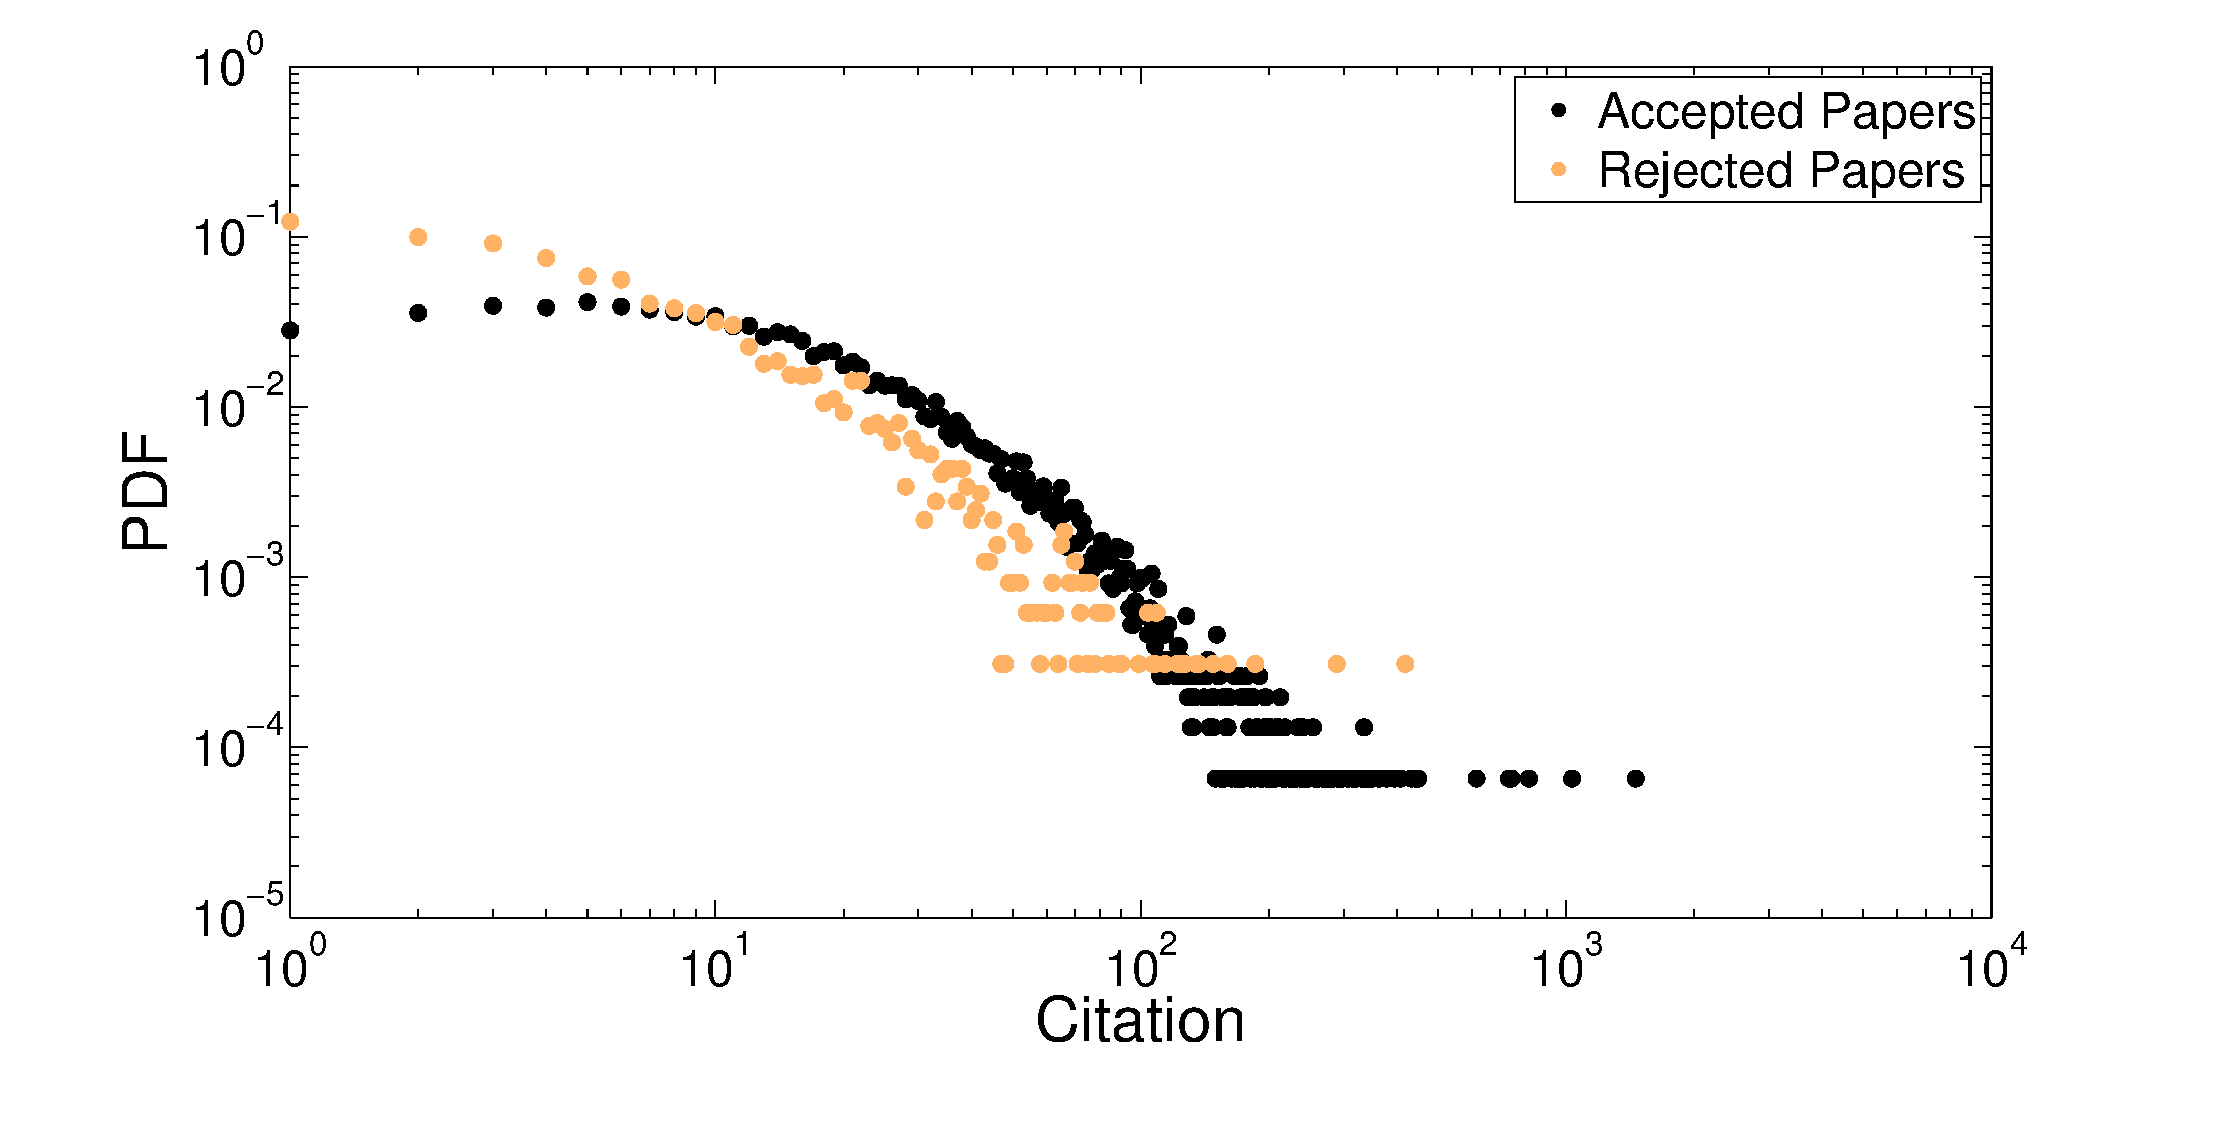
\includegraphics[scale=.12]{./texfiles/Chapter_4/jcdl/figures/citation_distribution.eps} & \includegraphics[scale=0.12]{./texfiles/Chapter_4/jcdl/figures/review_distribution.eps}
\end{tabular}
\caption{{\bf (Left)} Number of accepted and rejected papers per year from 1997 to 2015. {\bf (Middle)} Citation distribution of both the accepted and the rejected papers. {\bf (Right)} Distribution of number of reviews for accepted and rejected papers.}
\label{fig1}
\end{figure*}


The main aim of this work is to understand the importance of the review process and especially the contribution of the referees in this process. Such an analysis requires detailed information of reviews like the number of rounds of review, final decisions and the text of the review report in each round and, lastly, the number of citations for each paper. 

{\em Obtained data:} As stated earlier, for our analysis, we consider the dataset of the {\em Journal of High Energy Physics} (JHEP). It is one of the leading journals in its field and publishes theoretical, experimental and phenomenological papers. Among JHEP's most direct competitors there are Physical Review D, Nuclear Physics, EPJC, Physics Letters B and Physical Review Letters.
This dataset consists of {\bf 28871} papers that were submitted between 1997 (year of inception) and 2015 of which {\bf 20384} were accepted and {\bf 7073} were rejected. The rest of the papers were either withdrawn by the authors or the final decisions were not available. The number of distinct review reports is {\bf 70k} containing {\bf 12m} lines of review text. For each paper we have the title, the abstract, the authors, the date of publication (in case it was accepted) and the number of citations for the accepted papers. The dataset further contains for each paper the number of rounds of reviews it received before it was accepted (rejected) as well as the detailed text of the report submitted by the assigned reviewer and the editor.


\noindent{\em Pre-processing:} To obtain the necessary information for the rejected papers we queried the ``Inspire'' search engine\footnote{\url{https://inspirehep.net}} by their corresponding arXiv\footnote{\url{http://arxiv.org/}} ids. We could obtain for each paper the citation information, the abstract, the title, the authors and also the publishing journal (if at all it got published). Note that all through our analysis we refer to number of citations as the cumulative number of citations that a paper/author obtained at the end of 2015. 
We further had to disambiguate the names of the authors and assign each of them a unique id.  

\noindent{\em Some basic facts about the dataset:} In fig.~\ref{fig1}{\bf(Left)} we plot the year-wise distribution of the accepted and the rejected papers from 1997 to 2015. We observe an increasing trend in the number of submissions except for the year 2015 for which the data is incomplete. 
\begin{table}[htpb]
\centering
\caption{General information of the dataset.}
%\vspace{-2mm}
\label{tab1}
\begin{tabular}{|l|l|}
\hline
Number of papers                                                                 & 28871 \\ \hline
\hline
\begin{tabular}[c]{@{}l@{}}Number of papers (accepted)\end{tabular}            & 20384 \\ \hline
\begin{tabular}[c]{@{}l@{}}Number of papers (rejected)\end{tabular}            & 7073  \\ \hline
\begin{tabular}[c]{@{}l@{}}Average number of reviews (accepted papers)\end{tabular}   & 1.76  \\ \hline
\begin{tabular}[c]{@{}l@{}}Average number of reviews (rejected papers)\end{tabular}   & 1.35  \\ \hline
\begin{tabular}[c]{@{}l@{}}Average number of citations (accepted papers)\end{tabular} & 31.89 \\ \hline
\begin{tabular}[c]{@{}l@{}}Average number of citations (rejected papers)\end{tabular} & 9.45  \\ \hline
\end{tabular}
%\vspace{-2mm}
\end{table}
\begin{figure}
\centering
\includegraphics[scale=0.3]{./texfiles/Chapter_4/jcdl/figures/peer_review.jpg}
\caption{\label{peer_review} Peer-review system in JHEP}
\end{figure}
In fig.~\ref{fig1}{\bf(Middle)} we plot the citation distribution of the accepted and the rejected papers. Both the distributions seem to follow a power-law behavior. We further plot 
the distribution of the number of reviews for the accepted and the rejected papers in fig.~\ref{fig1}{\bf(Right)}. An important observation is that for JHEP, majority of the 
papers undergo one or two rounds of reviews after which they are either accepted or rejected. 
We note certain general information related to the dataset in table~\ref{tab1}.
Each submitted paper in the dataset also consists of the list of authors. There are {\bf 15127} unique authors in the dataset with at least one submission to JHEP and {\bf 12434} authors with at least one accepted paper. The average number of submissions per author is {\bf 5.18} while the number of authors per paper is {\bf 2.87}. 

\noindent{\em Peer-review process in JHEP:} For every submitted paper the administrator assigns an editor for it. The editor selects a single or a small set of reviewers for judging the quality of the contributions in the paper. The reviewer sends back his views in the form of a report. Based on this report the editor decides whether to accept or reject the paper. The editor may also ask the authors to reshape the paper based on the feedback of the reviewer(s) and in which case they have to resubmit before a decision on its acceptance could be taken. In fig.~\ref{peer_review}, we present a schematic showing the peer-review process in JHEP.

\medskip

% \documentclass[sigconf]{acmart}
% 
% \usepackage{booktabs} % For formal tables
% \usepackage{color}
% \usepackage{textcomp}
% \usepackage{booktabs}
% \usepackage{graphicx}
% \usepackage{todonotes}
% \usepackage{multirow}
% \usepackage{adjustbox}
% \newcommand\mycheck[1]{\textcolor{red}{#1}}
% Copyright
%\setcopyright{none}
%\setcopyright{acmcopyright}
%\setcopyright{acmlicensed}
%\setcopyright{rightsretained}
%\setcopyright{usgov}
%\setcopyright{usgovmixed}
%\setcopyright{cagov}
%\setcopyright{cagovmixed}


% DOI
%\acmDOI{10.475/123_4}

% ISBN
%\acmISBN{123-4567-24-567/08/06}

%Conference
%\acmConference[WOODSTOCK'97]{ACM Woodstock conference}{July 1997}{El
%  Paso, Texas USA} 
%\acmYear{1997}
%\copyrightyear{2016}

%\acmPrice{15.00}


% \begin{document}
% \title{Influence of Reviewer Interaction Network on Long-term Citations: A Case Study of the Scientific Peer-Review System\\ of the Journal of High Energy Physics}
% % \titlenote{Produces the permission block, and
% %   copyright information}
% % \subtitle{Extended Abstract}
% % \subtitlenote{The full version of the author's guide is available as
% %   \texttt{acmart.pdf} document}
% 
% 
% \author{Sandipan Sikdar}
% %\authornote{Dr.~Trovato insisted his name be first.}
% %\orcid{1234-5678-9012}
% \affiliation{%
%   \institution{Indian Institute of Technology Kharagpur}
%   %\streetaddress{P.O. Box 1212}
%   \city{Kharagpur,India} 
%   %\state{Ohio} 
%   \postcode{721302}
% }
% \email{sandipansikdar@cse.iitkgp.ernet.in}
% 
% \author{Matteo Marsili}
% %\authornote{The secretary disavows any knowledge of this author's actions.}
% \affiliation{%
%   \institution{International Centre for Theoretical Physics}
%   %\streetaddress{P.O. Box 1212}
%   \city{Strada Costiera} 
%   %\state{Ohio} 
%   \postcode{34014 Trieste, Italy}
% }
% \email{marsili@ictp.it}
% 
% \author{Niloy Ganguly}
% %\authornote{This author is the
% %  one who did all the really hard work.}
% \affiliation{%
%   \institution{Indian Institute of Technology Kharagpur}
%   %\streetaddress{P.O. Box 1212}
%   \city{Kharagpur,India} 
%   %\state{Ohio} 
%   \postcode{721302}
%   }
% \email{niloy@cse.iitkgp.ernet.in}
% 
% \author{Animesh Mukherjee}
% \affiliation{
%   \institution{Indian Institute of Technology Kharagpur}
%   %\streetaddress{P.O. Box 1212}
%   \city{Kharagpur,India} 
%   %\state{Ohio} 
%   \postcode{721302}}
% \email{animeshm@cse.iitkgp.ernet.in}
% 
% 
% \renewcommand{\shortauthors}{Sikdar et al.}
% 
% 
% \begin{abstract}
% A `peer-review system' in the context of judging research contributions, is one of the prime steps undertaken to ensure the quality 
% of the submissions received; a significant portion of the publishing budget is spent towards successful completion of the peer-review by the publication houses. Nevertheless, the scientific community is largely reaching a consensus that peer-review system, although indispensable, is nonetheless flawed.
% A very pertinent question therefore is ``could this system be improved?". 
% In this paper, we attempt to present an answer to this question by considering a massive dataset of around $29k$ papers with roughly $70k$ distinct review reports together 
% consisting of $12m$ lines of review text from the Journal of High Energy Physics (JHEP) between 1997 and 2015. In specific, we introduce a novel \textit{reviewer-reviewer interaction network} (an edge exists between two reviewers if they were assigned by the same editor) and show that surprisingly the simple structural properties of this network such as degree, clustering coefficient, centrality (closeness, betweenness etc.) serve as strong predictors of the long-term citations (i.e., the overall scientific impact) of a submitted paper. These features, when plugged in a regression model, alone achieves a high $R^2$ of \textbf{0.79} and a low $RMSE$ of \textbf{0.496} in predicting the long-term citations. In addition, we also design a set of supporting features built from the basic characteristics of the submitted papers, the authors and the referees (e.g., the popularity of the submitting author, the acceptance rate history of a referee, the linguistic properties laden in the text of the review reports etc.), which further results in overall improvement with $R^2$ of \textbf{0.81} and $RMSE$ of \textbf{0.46}. Analysis of feature importance shows that the network features constitute the best predictors for this task.   
% Although we do not claim to provide a full-fledged reviewer recommendation system (that could potentially replace an editor), our method could be extremely useful in assisting the editors in deciding the acceptance or rejection of a paper, thereby, improving the effectiveness of the peer-review system. 
% 
% \end{abstract}
% 
% 
%   \begin{CCSXML}
% <ccs2012>
% <concept>
% <concept_id>10010405.10010476.10003392</concept_id>
% <concept_desc>Applied computing~Digital libraries and archives</concept_desc>
% <concept_significance>500</concept_significance>
% </concept>
% <concept>
% <concept_id>10003120.10003130.10011762</concept_id>
% <concept_desc>Human-centered computing~Empirical studies in collaborative and social computing</concept_desc>
% <concept_significance>300</concept_significance>
% </concept>
% </ccs2012>
% \end{CCSXML}
% 
% \ccsdesc[500]{Applied computing~Digital libraries and archives}
% 
% 
% \keywords{citations; reviewer-reviewer interaction network; prediction;}
% 
% 
% \maketitle
% 
% %\noindent
\section{Introduction}
Information diffusion is one of the most common phenomena that occurs on a
network and the most elementary model of this process is SI
(Susceptible-Infected)~\cite{anderson1992infectious} and its different variations~\cite{watts2002simple,dodds2004universal,pnas1,pnas2,tang2009epidemic,son2012percolation}.
Epidemic/adoption models have recently found a renewed interest with the formulation of temporal networks and 
realization that most of the real-world networks are temporal in nature (network structure changes with time). 
\if{0}
For example,  Takaguchi et. al. in~\cite{takaguchi2013bursty} presents a model whereby adoption behavior 
of a node is driven by the number of recent contacts with already adopted individual. 
Through simulations on real-world temporal networks the authors further show that burstiness~\cite{karsai2011small} 
affects spreading rate. Similar empirical study was also performed by Karimi et. al. in~\cite{karimi2013threshold}. A further modification to the 
model has been proposed by Backlund et. al. in~\cite{backlund2014effects} which considers that adoption is driven by the number of contacts
with different adopted neighbors within a chosen time instead of a particular neighbor multiple times. Further, information diffusion on temporal 
networks, more specifically prevalence, have also been studied in \cite{rocha2013bursts}. 
Several other results on the study of 
epidemics in temporal networks are listed in~\cite{masuda2013predicting} and on epidemic thresholds in~\cite{prl1,van2012epidemic,zhang2014susceptible}.
This type of history-dependent thresholding spreading pattern is largely observed in spread of bacterial diseases such as tuberculosis and 
dysentery \cite{joh2009dynamics} and 
also in peer-to-peer \cite{sanghavi2007gossiping} and Bittorrent systems \cite{qiu2004modeling}. In \cite{romero2011differences} the authors show that people 
accept ideas/news after repeated exposure.
\fi

The fundamental difference between static and temporal epidemic (SI) models is that in temporal models every agent  within a population is {\em not equally susceptible} to a disease or equally amenable to a rumor
 - the one which has been exposed more number of times (in recent past) are more amenable. This difference however is not well formulated and hence not well modeled - the primary contribution of this work 
is to succinctly define the problem in  terms of a simple model and then theoretically calculate the rate of spread of the epidemics. 
%Albeit a deep literature exists on the study of epidemics in temporal networks, they are mostly simulation based and to the best of our knowledge, a theoretical foundation on the topic is still wanting. 
We consider a spreading model in the lines of~\cite{takaguchi2013bursty} where each susceptible node needs to communicate with the 
infected nodes {\em multiple times} to contract infection. More importantly, unlike memoryless systems, we assume that each node comprises a memory which 
keeps track of the number of contacts it makes with infected ones. Note that in our system memory is a property which allows each node to remember the number 
of contacts it has already made with the infected ones. While Karimi et. al. studied the effect of burstiness in the diffusion process, we 
are more interested in estimating both empirically and analytically the diffusion time and rate.
Note that this model is completely different from  threshold models~\cite{granovetter1978threshold,sur1} where a node
 gets infected when majority of its neighbors are infected or probabilistic SI-models where an infected node,  on coming in contact, 
infects a susceptible node with a probability $p$,  as those are memoryless systems and the transition depends only on the activity of present time step. 
Our diffusion model also differs from the Neighborhood Exchange (NE) model proposed in \cite{volz2007susceptible}. NE assumes at any given time, an individual
will be in contact with an individual-specific number of neighbors with whom disease transmission is possible while our model considers that a node can be in contact with 
only a single individual. Also NE does not consider the fact that multiple contacts are required to contract infection.

The analytical results are obtained 
considering simple yet important topologies like the complete graph and the infinite $d$-regular trees which accounts for two extreme variants of network topology in terms of edge 
density. 
We demonstrate that the total diffusion time required for complemete graph topology (with $n$ nodes) scales as $n^{\frac{k-1}{k}}$ where $k>1$ is the number 
of contacts required to infect a susceptible individual. 
This is in sharp contrast to the case with $k$ = $1$, where it has been shown that diffusion time 
scales as $\log{(n)}$ ~\cite{rumarSreadingPushPull,rumourSpreading_evolvingGraph_PushPull}.
Another important inference we draw from the theoretical analysis is that irrespective of the topology the diffusion process could be divided into two phases: (i) an initial phase where the diffusion rate is very slow and 
(ii) a residual phase where the diffusion becomes very fast.
This inference is also a crucial contribution of this work which can help in containing 
the spread of infectious diseases with minimum overhead if acted upon in the initial phase which we further prove through a detailed empirical study.


\medskip

% \vspace{-4mm}

In this section, we concentrate on our first task which is predicting the long term impact of a paper in terms of citations. 
In specific, we construct a reviewer-reviewer interaction network and show that its properties are linked to the future scientific impact of a paper.  
We hypothesize that the position of the assigned reviewer in the network (measured in terms of degree, centrality, clustering coefficient and PageRank) 
could be used to predict the long term citation of the paper. Additionally, we design a set of supporting features specific to paper, author, review report and reviewer to 
further improve our prediction model. 


\noindent
\section{Reviewer-reviewer interaction network}
\label{rev_int_net}
In this section, we construct a reviewer-reviewer interaction network and show that its properties are linked to the future scientific impact of a paper (measured in terms of the cumulative citation count). In specific, we find that the position of the assigned reviewer in the network (measured in terms of degree, centrality, clustering coefficient and PageRank) could be used to predict the long term citation of the paper. 
 
The reviewer-reviewer interaction network is created with each node representing a reviewer and an edge exists between two reviewers if they have been assigned by at least one common editor. We devote the rest of the section in demonstrating the importance of the various structural properties of the network in determining the long term citation of the paper. Note that there are 4035 unique reviewers in the system each of which form a node in this network.

\begin{figure*}
\centering
\includegraphics[width = 0.9\textwidth]{./texfiles/Chapter_4/jcdl/figures/citation_.eps} 
\caption{\label{fig:net_citation} Cumulative distribution function (CDF) of citations received by the papers (accepted) reviewed by referees in top 25\% and bottom 25\% reviewers ranked according to (a) degree, (b) betweenness centrality, (c) closeness centrality (d) clustering coefficient values and (e) PageRank in the reviewer-reviewer interaction network.\vspace{4mm}}
\end{figure*}

\subsection{Degree (Deg)}
Degree of a node $v$ is the number of other nodes it is connected to in the network. A node with a higher degree in the reviewer-reviewer interaction network would indicate (i) assignment from multiple editors, (ii) assignment from a reputed editor (with large number of assignments) which in turn would indicate the reputation of the reviewer. To verify our hypothesis, we rank the reviewers based on their degree in the network and calculate the mean citation of the papers reviewed by the reviewers in the top and the bottom 25\% of the rank list. We observe that  the papers reviewed by the top 25\% reviewers receive much higher citations than the those reviewed by the bottom 25\% reviewers (refer to fig.~\ref{fig:net_citation}(a)).    

\subsection{Betweenness centrality (BC)}

Betweenness centrality of a node quantifies the position of a node based on the number of shortest paths the node is part of. For every  pair of nodes in the network there exists a shortest path between them. Betweenness centrality of a node ($v$) is the fraction of all such paths that pass through $v$. In the reviewer-reviewer interaction network, a high  centrality value would indicate assignment by multiple editors and that this node acts as a bridge between them. We again rank the reviewers based on the betweenness centrality values and calculate the average citation of the papers. We find that the papers accepted by the top 25\% reviewers tend to be cited more compared to those accepted by the bottom 25\% (refer to fig.~\ref{fig:net_citation}(b)). 

\subsection{Closeness centrality (CC)}

Formally closeness centrality of a node in a network is the inverse of the sum of length of its shortest path to all other nodes in the network. Hence higher centrality value indicates that the node is more closer to all other nodes in the network. In the reviewer-reviewer interaction network, a reputed reviewer will be assigned by multiple reviewers and hence will be closer to the other reviewers in the network. This is represented in fig.~\ref{fig:net_citation}(c), where we show that the papers accepted by top 25\% most central reviewers 
are cited more often compared to the bottom 25\% reviewers. 

\subsection{Clustering coefficient (Clus)}

Clustering coefficient of a node is measured as the fraction of connections among the neighbors of the node. For the reviewer-reviewer interaction network, every reviewer assigned by a common editor is connected to every other reviewer in the network. A reviewer assigned by many editors would actually act as a bridge between two cliques and hence would have a lower clustering coefficient value compared to a reviewer who is part of a single clique (always assigned by a single editor). This is further demonstrated in  fig.~\ref{fig:net_citation}(d) where we observe that the papers accepted by reviewers having lower clustering coefficient tend to be cited more.

\subsection{PageRank (PR)}

PageRank is a link analysis based algorithm that calculates for each node its relative importance within 
the network. Specifically, PageRank outputs a probability distribution which is used as the likelihood of a random walker to end up in a specific node. We simulate PageRank on the reviewer-reviewer interaction 
network to obtain the relative importance of each node. Further analysis indicates that the papers accepted by the top 25\% reviewers (based on PageRank) are cited more often compared to those accepted by the bottom 25\% reviewers (refer to fig.~\ref{fig:net_citation}(e)). 

The above results thus indicate that simple network properties of the reviewer-reviewer interaction network could be highly effective in predicting the long-term citation of the paper at the time of publishing. 
\medskip


\noindent
\subsection{Supporting features}
Most of the works~\cite{yan2012better,chakraborty2014towards} related to predicting long-term citation of papers considers a wide set of author related features, papers-centric features and citation pattern of the paper in the first few years from the date of its publication. 
Further, our dataset allows us (unlike the existing datasets) to look into several other features related to the review-process like the review report, the behavior of the assigned referee, the number of rounds of reviews the paper went through and others. 
We consider the above features as well as those existing in the previous literature (wherever available) as the set of supporting features. The features are categorized into (i) paper based, (ii) review report based, (iii) author based and (iv) reviewer based. Apart from investigating the effectiveness of a feature in determining the long-term citation of the paper, we also point out some interesting observations that we could make while analyzing the dataset.    

\subsubsection{Paper based features}
\label{analysis}
We have already observed that the average number of citations received by accepted papers is 31.80; for rejected papers the corresponding value is 9.45 (refer to table~\ref{tab1}). Note that for each paper we consider the citations accrued by it till 2015 from the date of publication.
We further consider all the accepted and the rejected papers and segregate them based on the number of citations received. We consider different citation buckets and plot the fraction of accepted and rejected papers in each of these buckets in figure~\ref{fig4} {\bf (Left)}. Note that the bucket sizes are in increasing powers of 2. Typically, the buckets are $\leq 1$, $2$, $(>2$ and $\leq 4)$ and so on. It can be clearly observed that accepted papers are cited more often compared to the rejected ones. Nevertheless, on further analysis we find that there could be a few exception cases where the rejected paper could make a place in higher impact journals (compared to JHEP) and, eventually, receive a high volume of citations in future. We present two such pathological cases below -- {\bf Case 1:} Rejected after two rounds of review, later accepted at Physics Letters B, citations: 1209; {\bf Case 2:} Rejected after one round of review, later accepted at Computer Physics Communications, citations: 929. We perform a thorough analysis of these irregular cases later in the paper.



\subsubsection*{Number of review rounds (RR)}

 \begin{figure*}[htpb]
 \centering
 %\vspace{-4mm}
 \begin{tabular}{ccc}
 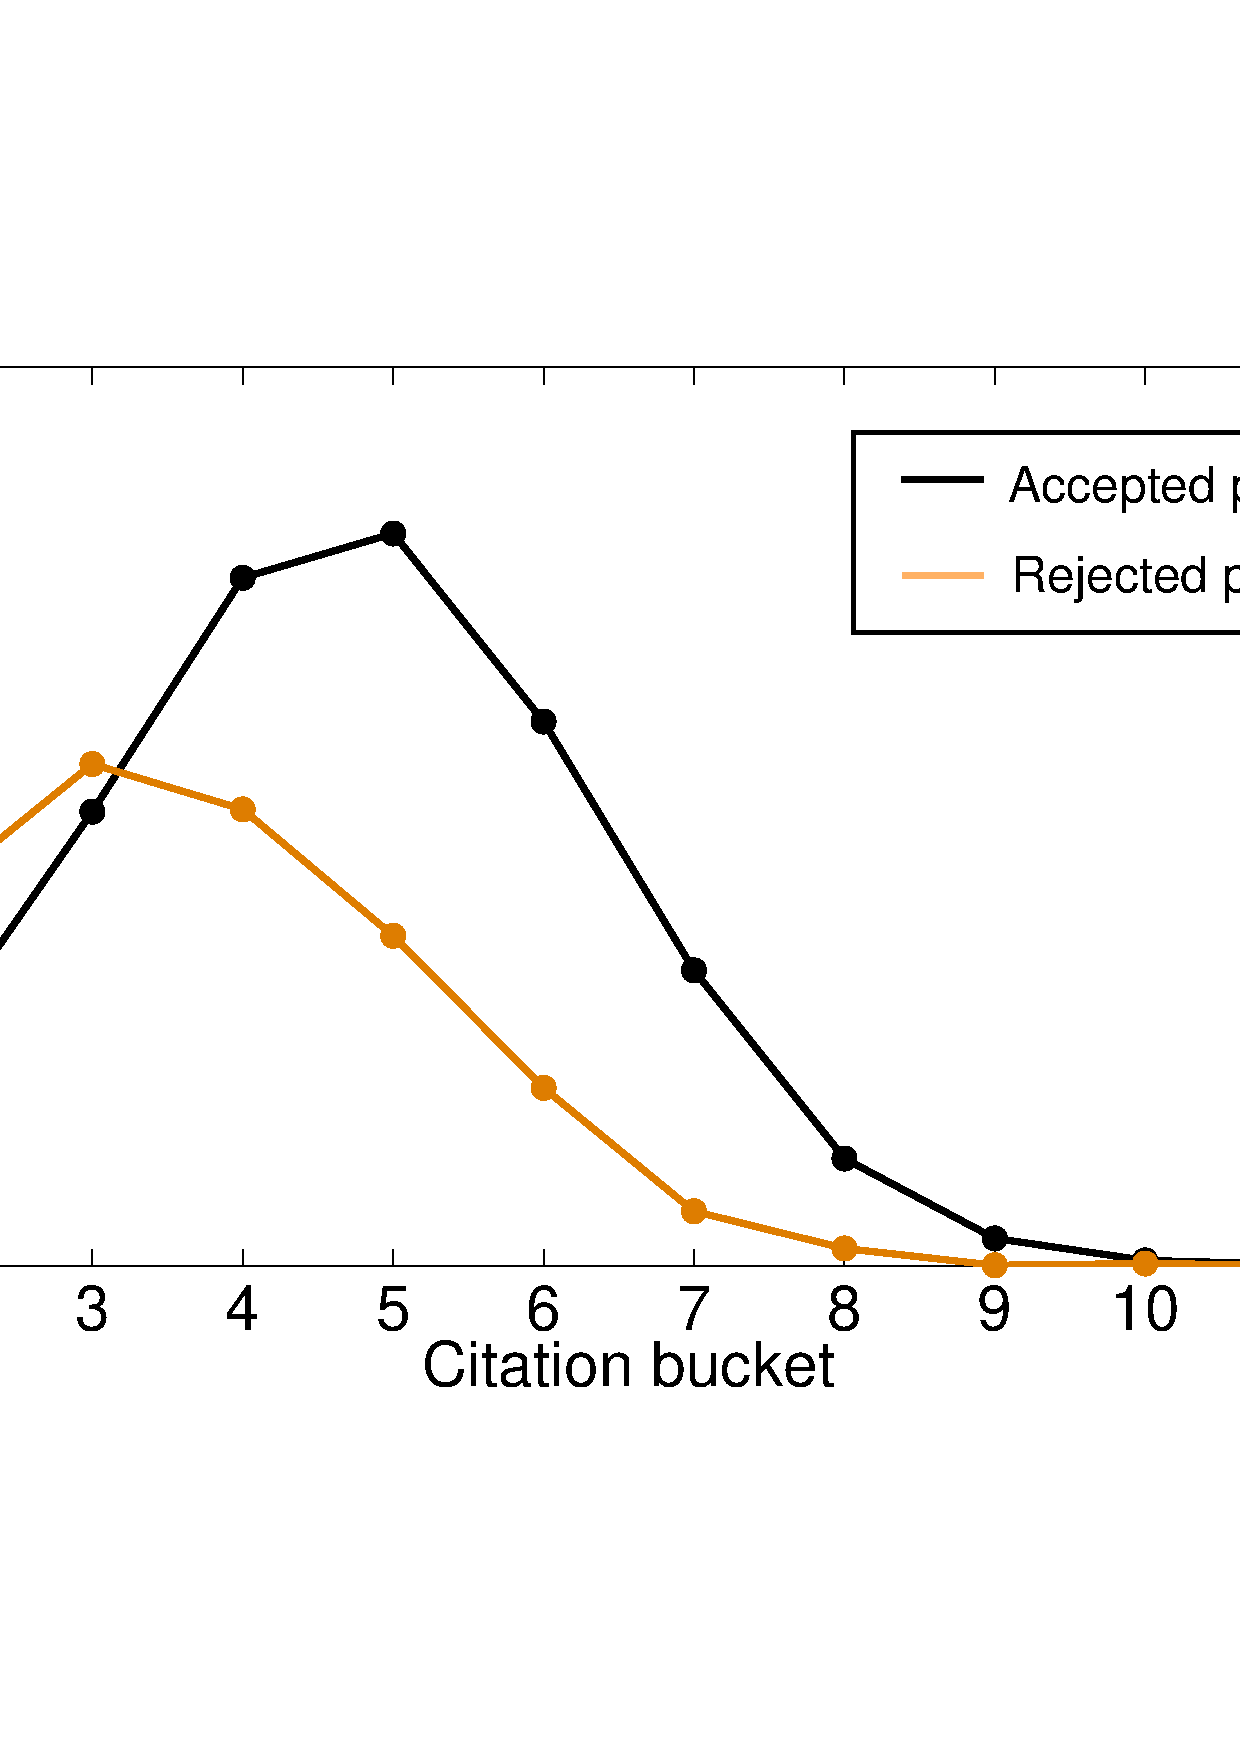
\includegraphics[scale=0.12]{./texfiles/Chapter_4/jcdl/figures/citation_bucket_frac_paper} & \includegraphics[scale=0.12]{./texfiles/Chapter_4/jcdl/figures/citation_bucket_reviews_all-eps-converted-to.pdf} & \includegraphics[scale=0.12]{./texfiles/Chapter_4/jcdl/figures/cit_rnd_rev-eps-converted-to.pdf}
 \end{tabular}
  \caption{{\bf (Left)} Fraction of accepted and rejected papers in different citation buckets. {\bf (Middle)} Average number of reviews for accepted and rejected papers in different citation buckets. For both {\bf (Left)} and {\bf(Middle) } bucket sizes are in increasing powers of 2. E.g. $\leq 1$, $2$, ($>2$ and $\leq 4$) and so on. {\bf (Right)} Average citation of the top 20 percentile  papers for a given number of rounds of review request.}
   \label{fig4}
   \vspace{4mm}
 \end{figure*}


We next check whether the {\bf review rounds} improve the quality of the paper. To this aim we segregate the papers based on the number of citations into different buckets and for each bucket we calculate the average number of reviews the papers received in that bucket. The bucket sizes are again in increasing powers of 2. Typically, the buckets are $\leq 1$, $2$, $(>2$ and $\leq 4)$ and so on. We plot the results in figure~\ref{fig4} {\bf (Middle)}. We observe that for accepted papers, the low cited ones on average tend to get accepted after more rounds of reviews while the high cited ones undergo lesser rounds of reviews before getting accepted. It can hence be concluded that going through the review process multiple times does not necessarily improve the quality of the papers much that are eventually accepted. For the rejected papers we observe a contrasting trend indicating that the review process indeed helped in improving the quality of the paper in the long run possibly enhancing the chances of its acceptance at a different venue later. For the accepted papers we further classify them based on the number of reviews they received and calculate the average citations of the top 20 percentile papers (ranked by citations) in each class (refer to figure~\ref{fig4} {\bf (Right)}). We observe that the average citation drops as the number of reviews increases further suggesting that papers accepted after higher number of reviews often fail to create a high citation impact. This indicates that the number of rounds of review could be an indicator of the long-term citation of the paper. 

\begin{figure}
\centering
\includegraphics[scale  = 0.25]{./texfiles/Chapter_4/jcdl/figures/team_citation}
\caption{\label{team:citation} Average citation versus team size. Note that we segregate the papers based on the teams size and calculate the average citation.}
\vspace{4mm}
\end{figure}


\subsubsection*{Team size (TS)}
The authors in~\cite{chakraborty2014towards} hypothesized that there exits an optimal team size for which the citations received by the paper is maximum. We hence segregate the papers based on the team size and calculate the mean citation of the papers. We observe that team size 9 (refer to figure~\ref{team:citation}) is the optimal as the papers with 9 authors gets more citation on average.

\medskip


\begin{figure}
\centering
\includegraphics[scale=0.25]{./texfiles/Chapter_4/jcdl/figures/len_citation.eps}
\caption{Mean length of referee reports in terms of number of words at different rounds of review. Typically the buckets are $< 100$, ($\geq 100, < 200$) and so on}
\label{fig:length}
\end{figure}


\subsection{Review report based features}
\label{text_analysis}

In this subsection we analyze whether certain features could be extracted from the reports sent by the reviewers that could be an indicator of the long-term citation of the paper. Note that we have two types of reports -- {\bf Referee report}: Report sent by the assigned referee to the editors and {\bf Editor report}: Report sent by the editor to the authors based on the referee report. We primarily focus on the referee reports as editorial reports are in almost all cases a reiteration of the referee reports.

\subsubsection{Length of the reports (RL)}
We start by looking whether the length of the review reports sent by the reviewers are indicative of the quality and hence the long-term citation of the paper. To this aim we segregate the papers based on the length of the report and calculate the mean citation of each of these buckets. The lengths are bucketed with sizes typically $< 100$, ($\geq 100, < 200$) and so on. We observe that there exists an optimal length (between 500 and 600 words) for which the citation obtained by the corresponding paper is maximum  (refer to figure \ref{fig:length}). 


\subsubsection{Sentiments (SNT)}
We next perform sentiment analysis on the review reports. To determine the sentiment of a report we use a method described in~\cite{montejo2012random} which performs a graph-based word sense disambiguation and lexical similarity analysis using a pre-existing knowledge base. A sentiment score of 0 indicates that the document is neutral, a positive score  indicates a positive sentiment and a negative score indicates a negative sentiment. 


\begin{figure}[htpb]
\centering
%\vspace{-5mm}
\includegraphics[scale=0.23]{./texfiles/Chapter_4/jcdl/figures/year_sent_cit-eps-converted-to.pdf}
\caption{Sentiment score versus citations for both accepted and rejected papers for the years 2005, 2007 and 2009. We find similar trends for other years as well.}
\label{fig12}
\end{figure}

To determine whether the overall sentiment of the reviews of a paper is related to the number of citations received by it, we plot for each paper (both accepted and rejected) the number of citations it received against the  sentiment score of the first round of review in fig.~\ref{fig12}. Note that we segregate the papers based on the year of the publication or the rejection. We observe that the highly cited papers mostly have reviews with neutral or positive sentiment. Accepted papers with positive reviews are, on average, found to receive $25.27$ citations while those with negative reviews are found to receive $13.56$ citations.
However, there are cases where the accepted paper received highly positive reviews but was not cited. Conversely, there are cases where the sentiment was neutral but the paper garnered a large number of citations. Shown below are two such examples -- {\bf Case 1:} Year of publication: 2006, sentiment score: 0.0234 (almost neutral), citations: 5812; {\bf Case 2:} Year of publication: 2008, sentiment score: 0.65 (highly positive), citations: 6.


For the rejected papers we observe that those which received neutral reviews but were rejected, tend to garner higher citations later compared to the ones which received negative reviews. There are certain exceptions as well, two of which are -- {\bf Case 1:} Year of rejection: 2010, sentiment score: 0.27 (positive), citations: 1; {\bf Case 2:} Year of rejection: 2007, sentiment score: -0.14 (negative), citations: 711.
Manual investigation of the review text shows that the papers which are highly cited after rejection were mainly rejected for not being in the scope of JHEP and not because of flawed results. 

\subsubsection{Linguistic quality indicators (LQI)}

Here we check whether there are linguistic quality features present in the review reports which can serve as an indicator of the future impact of the paper. To our aim we use the LIWC\footnote{\url{http://liwc.wpengine.com/}} (Linguistic Inquiry and Word Count) text analysis tool~\cite{pennebaker2007development}. The tool provides, as output, percentage of words in different categories for an input text. The categories are broadly divided into linguistic (21 dimensions like pronouns, articles etc.), psychological (41 dimensions like affect, cognition etc.), personal concern (6 dimensions), informal language markers and punctuation apart from some general features like word count, words per sentence etc. We apply the LIWC tool on the review reports for our analysis and mainly focus on the linguistic and the psychological categories.
Next we check whether the LIWC features discussed earlier can also serve as indicators differentiating high and low cited papers. We rank the papers based on the number of citations they have received and consider the top 10\% as highly cited and the bottom 10\% as low cited papers. Note that we only consider the papers that were published before 2012 so that the papers have at least three years of citation history. In table~\ref{tab3} we report the mean percentage of words in different LIWC categories across all the papers (both high and low cited). We find several quality indicators here as well. The key observations are: (i) future tense is used more significantly in case of review reports of highly cited papers compared to low cited papers. On manually investigating the reviews of some of the highly cited papers we observe that statements like ``its result will become a useful addition to ..'' are prevalent; (ii) insightful and inclusive words are also used to a greater extent in review reports of highly cited papers compared to low cited papers; (iii) positive words are also more prevalent in highly cited papers as well.\\
Thus, these indicators show that the reviewers were, in many cases, indeed able to guess the quality of the paper as is evident from the review reports.

\begin{table}
\centering
\caption{Mean values of percentages of various categories of words in review reports of high and low cited papers where the means differ significantly.\vspace{3mm}}
\label{tab3}
\begin{tabular}{|l|l|l|l|}
\hline
Category                    & Dimension                                                   & \begin{tabular}[c]{@{}l@{}}High cited\\ papers\end{tabular} & \begin{tabular}[c]{@{}l@{}}Low cited\\ papers\end{tabular} \\ \hline \hline
\multirow{2}{*}{Linguistic} & Future tense                                                & 1.17                                                          & 1.05                                                         \\ \cline{2-4} 
                            & Negation                                                    & 0.72                                                          & 0.84                                                         \\ \hline
\multirow{4}{*}{Cognitive}  & Insight                                                     & 3.52                                                          & 3.16                                                         \\ \cline{2-4} 
                            & Causation                                                   & 2.60                                                          & 2.38                                                         \\ \cline{2-4} 
                            & Inclusive                                                   & 3.70                                                          & 3.43                                                         \\ \cline{2-4} 
                            & Exclusive                                                   & 1.28                                                          & 1.52                                                         \\ \hline
Affective                   & \begin{tabular}[c]{@{}l@{}}Positive \\ emotion\end{tabular} & 2.84                                                          & 2.70                                                         \\ \hline
\end{tabular}
\vspace{2mm}
\end{table}



\noindent
\subsection{Author based features}
\label{author_analysis}

We next look into some of the author based features like author reputation and author productivity to determine how they influence the long-term citation of the paper.  
\begin{figure*}
\centering
\begin{tabular}{ccc}
\includegraphics[scale=0.15]{figures/citation_succes_ratio.eps} & \includegraphics[scale=0.15]{figures/review_succes_ratio.eps} & \includegraphics[scale=0.15]{figures/sentiment_succes_ratio-eps-converted-to.pdf}
\end{tabular}
\caption{{\bf (Left)} Mean number of citations per paper versus acceptance ratio. {\bf (Middle)} Mean number of reviews per paper versus acceptance ratio. {\bf (Right)} Mean sentiment score per paper versus acceptance ratio. Note that in each case we use acceptance ratio buckets where buckets correspond to acceptance ratio ($\geq 0.1$ and $< 0.2$), ($\geq 0.2$ and $<0.3$) and so on.}
\label{fig13}
\end{figure*}
\subsubsection{Author reputation (AR)} We analyze whether there are some specific authors whose papers always get accepted and similarly there are others whose papers always get rejected.  
For each author we define a metric called {\bf acceptance ratio} which is the fraction of submitted papers accepted in JHEP. Formally, acceptance ratio of an author $i$ is defined by: $acceptance\,ratio_{i}=\frac{accept_{i}}{accept_{i} + reject_{i}}$.    
where $accept_{i}$ and $reject_{i}$ represents respectively the number of accepted and rejected papers of the author $i$ in JHEP. We use this metric as a proxy for author reputation.
We observe that mean acceptance ratio across all the authors is $0.56$. In fact, for almost 7\% of the authors, the acceptance ratio is 1. Next we check whether the authors with high acceptance ratio have higher citations per paper. To this aim we segregate authors based on the acceptance ratio and calculate the mean number of citations per paper for these authors (refer to fig.~\ref{fig13}{\bf (Left)}). We observe an increasing trend suggesting that the authors with higher acceptance ratio tend to have higher citations. 
\begin{figure}
\centering
\includegraphics[scale=0.25]{figures/prod_citation.eps}
\caption{Mean citation of the papers versus the average time(in days) between two submission. Note that  we use time buckets where buckets correspond to $<100$,($\geq 100$ and $< 200$), ($\geq 200$ and $<300$) and so on.\vspace{-2mm}}
\label{fig:prod}
\end{figure}

To check whether the authors having higher acceptance ratio are also reviewed less, we again segregate the authors based on the acceptance ratio and calculate the average number of reviews received per paper for these authors (refer to fig.~\ref{fig13}{\bf (Middle)}). We observe a decreasing trend implying that papers of authors with higher acceptance ratio are indeed reviewed less. Although there are authors with high acceptance ratio whose papers are reviewed less, they are often highly cited indicating the overall effectiveness of the review process. We further study the sentiment score of the review reports for authors with different acceptance ratios. For authors in a given  acceptance ratio bucket we calculate the average sentiment score of the review reports of their papers.
We observe that the authors having higher acceptance ratios tend to have more positive reviews on average compared to the others with lower acceptance ratios which is indicated by the increasing trend in the curve in fig.~\ref{fig13}{\bf (Right)}. 

\subsubsection{Author productivity (AP)} It is established in the literature \cite{yan2012better} that the more papers an author publishes, more are his chances of getting cited. We hence use it as a feature in predicting the long-term citation of the paper. We calculate for each author the mean time ($s_t$) between two submissions. We use $s_t$ as proxy for author productivity as low $s_t$ would indicate higher productivity rate and vice versa.  
The papers are segregated based on the corresponding author's $s_t$ and then the mean citation is calculated. Each bucket correspond to $<100$,($\geq 100$ and $< 200$), ($\geq 200$ and $<300$) and so on. We observe that more frequent the submission, more is the chance of getting citation (refer to figure \ref{fig:prod}).


%\medskip

\noindent
\subsection{Reviewer based features}
\label{reviewer_analysis}

The success of the peer-review process is immensely dependent on the reviewers as they determine the quality of a paper and, consequently, the quality of the journal. We hence investigate certain reviewer behaviors (pointed out in~\cite{sikdar2016anomalies}) that could  be indicative of his/her performance.

\subsubsection{Accept ratio (RAC)} For each reviewer we define a metric called accept ratio (this is different from the acceptance ratio defined in the previous section) Formally, the {\bf accept ratio} for reviewer $j$ is $accept\,ratio_{j}=\frac{accept_{j}}{accept_{j} + reject_{j}}$ 
where $accept_{j}$ and $reject_{j}$ respectively represent the number of papers reviewer $j$ accepted and rejected. The mean accept ratio across all the reviewers is $0.62$. An accept ratio of 1 for a reviewer would mean that he accepted all the papers that were assigned to him.

\begin{figure*}
\centering
\begin{tabular}{ccc}
\includegraphics[scale=0.15]{figures/reviewer_citation_ratio-eps-converted-to.pdf} & \includegraphics[scale=0.15]{figures/reviewer_review_ratio-eps-converted-to.pdf} & \includegraphics[scale=0.15]{figures/reviewer_sentiment_ratio-eps-converted-to.pdf}
\end{tabular}
\caption{{\bf (Left)} Mean number of citations per paper versus accept ratio. {\bf (Middle)} Mean number of reviews per paper versus accept ratio. {\bf (Right)} Mean sentiment score per paper versus accept ratio. Note that in each case we use accept ratio buckets where the buckets correspond to accept ratio ($\geq 0.1$ and $< 0.2$), ($\geq 0.2$ and $<0.3$) and so on.}
\label{fig16}
%\vspace{-3mm}
\end{figure*}


We start by investigating how well the reviewers were able to anticipate the quality of the paper. To this aim we segregate papers based on their assigned reviewer's accept ratio and calculate the mean number of citations received. In fig.~\ref{fig16}{\bf (Left)} we plot the number of citations per paper given the accept ratio of the assigned reviewer. We observe that most cited papers were reviewed by reviewers with accept ratio between 0.6 and 0.7. Surprisingly, the papers reviewed by reviewers with very low and very high accept ratio tend to garner less citations. This indicates that some papers could have been accepted just because the assigned reviewer is oriented to accept most of the papers. In fact, manual inspection indicates that many of the rejected papers that garnered large number of citations later on were mostly reviewed by reviewers with low accept ratio. We further investigate the number of reviews a reviewer with a given accept ratio suggests before he accepts or rejects a paper. For this we again segregate the papers based on the assigned reviewers accept ratio and calculate the number of rounds of reviews, these papers received on average. We present the results in fig.~\ref{fig16}{\bf (Middle)}. Since in most of the cases the same reviewer is assigned in each round of review, we observe that reviewers with a low accept ratio tend to recommend more rounds of reviews while those with higher accept ratio tend to suggest lesser number of review rounds. This indicates that the reviewers with low accept ratio often fail to improve the quality of the paper as is evident from the mean number of citations these papers receive albeit dragging the paper through multiple rounds of reviews.


To complete the analysis we also investigate the average sentiment score of the papers based on the accept ratio of the assigned reviewers. In fig.~\ref{fig16}{\bf (Right)} we plot the average sentiment score of the papers with similar accept ratio of the assigned reviewer. We observe an increasing trend indicating that the reviewers with very high accept ratio always tend to give more positive reviews as compared to others with lower accept ratio. \iffalse Note that we also repeat the analysis for the small set of editors separately; in all cases the results show exactly similar trends as in case of reviewers.\fi 


\begin{figure}
\centering
\includegraphics[scale = 0.28]{figures/rev_all.eps}
\caption{\label{fig:rev} Mean citation of the papers versus (a) time since the last assignment for the assigned reviewer and (b) time taken by the reviewer to send the report. Note that for both the cases the times are divided into equi-sized buckets. For (a) bucket sizes are 100 each while for (b) it is 25.}
\end{figure}

\subsubsection{Time since last assignment (TA)}

In lines of~\cite{sikdar2016anomalies} we consider the time (in number of days) since the last assignment for the assigned reviewer as an indicator of reviewer's performance and hence an indicator of the long-term citation of the paper. To verify our hypothesis we segregate the papers based on the assigned reviewer's time till last assignment and calculate the mean citation. The times are bucketed with bucket size typically $< 100$, ($\geq 100, < 200$) and so on. We observe in fig.~\ref{fig:rev}(a) that there does exist an optimal time for which the citation of the accepted paper is maximum. Further if the time since last assignment is too low or too high the long-term citation is low.   

\subsubsection{Delay in submitting the report (DR)}

We further check whether the time taken by the assigned reviewer in submitting the report is also as an indicator for his performance and hence that of the long-term citation of the paper. To this aim we calculate for each paper the time between assigned reviewer acknowledging to review the paper and the reviewer sending back the report. The papers are segregated based on this time and then the mean citation is calculated. 
The times were binned with typical bucket sizes being $>25$, $(\geq 25, < 50)$ and so on. We observe from fig.~\ref{fig:rev}(b) that the citation is maximum when the reviewer sent back the report between 50 and 75 days. The citations are comparatively less if the time is too high as well as too low. 

\medskip




%\vspace{-8mm}
\subsection{Prediction results}
\label{performance_measure}

\begin{table*}[]
\centering
\caption{The F-statistics value for all the features used for predicting the long-term citation of the paper.}
\label{tab:f_score}
 \begin{adjustbox}{max width=\textwidth}
\begin{tabular}{|l|l|l|l|l|l|l|l|l|l|l|l|l|l|l|}
\hline
Feature      & Deg  & BC    & CC    & Clus  & PR    & RR   & TS   & RL   & SNT  & AR    & AP    & RAC  & TA   & DR   \\ \hline
F-statistics & {\bf 26.1} & {\bf 29.21} & {\bf 27.72} & {\bf 17.82} & {\bf 23.34} & 6.17 & {\bf 25.6} & 14.1 & 0.94 & {\bf 18.52} & {\bf 16.49} & 3.49 & 8.68 & 7.59 \\ \hline
\end{tabular}
\end{adjustbox}
\vspace{4mm}
\end{table*}

\begin{table*}[]
\centering
\caption{The F-statistics value for all author related features for predicting the long-term citation of the paper.}
\label{tab:fscore_author}
\begin{tabular}{|l|l|l|l|l|l|l|l|l|}
\hline
Features     & AS   & AC    & AF    & Age   & AAR   & ACD   & ACA   & ATD   \\ \hline
F-statistics & 26.3 & 19.23 & 18.67 & 25.42 & 22.15 & 25.78 & 23.32 & 17.68 \\ \hline
\end{tabular}
\vspace{4mm}
\end{table*}

In this section we design a regression model to calculate the long-term citation impact of a paper. 
We perform our prediction for papers that were accepted in JHEP between 2007 and 2012. Note that for each paper, its citation till 2015 is available. Hence papers published in 2004 would have a higher citation on average compared to papers which were published in 2010 (say) due to higher exposure time. Thus, instead of calculating  the exact citation value we predict the citation rank (for each year we rank the papers based on the citations they have accrued till 2015). Further note that the papers are sorted based on the date of submission and given a paper we construct the reviewer-reviewer interaction network until its submission date (excluding). This ensures that there is no data leakage. Similarly for supporting features like acceptance ratio of an author we consider information only up to his/her last submission. 

\noindent{\bf Network features only:} Considering only the network features, we obtain the best result using support vector regression (RBF kernel) with parameters $C=100$ and $\gamma=0.01$. We perform a 10-fold cross-validation and obtain a high $R^2$ of {\bf 0.79} and a low $RMSE$ of {\bf 0.496}. 

\noindent{\bf Network + supporting features:} Considering both the network and the supporting features we obtain a further overall improvement. In specific, using support vector regression (RBF kernel) we obtain a high $R^2$ of {\bf 0.81} and a low $RMSE$ of {\bf 0.46}. In this case we set the parameters $C=100$ and $\gamma=0.02$. We further calculate the $F$-Statistic values for all the features used in the regression task (refer to tables~\ref{tab:f_score} and \ref{tab:fscore_author}) and observe that the network features, are in general, are more suited to the task of prediction.


Thus our system is correctly able to predict the citation rank of the paper. We believe our system could be useful in assisting the editors in deciding whether to accept or reject the papers especially in cases where the reports are contradictory. 
\medskip



\noindent
%\vspace{-3mm}
\section{Irregular cases}

\begin{figure}
\centering
\includegraphics[scale=0.17]{figures/highly_cited_rejected-eps-converted-to.pdf}
\caption{CDF of (a) acceptance ratio of authors and (b) accept ratio of reviewers for accepted papers and highly cited rejected papers.\vspace{-4mm}}
\label{fig10}
%\vspace{-1mm}
\end{figure}

\begin{figure}
\centering
\includegraphics[scale=0.17]{figures/low_cited_accepted-eps-converted-to.pdf}
\caption{CDF of (a) accept ratio of reviewers, (b) acceptance ratio of authors (c) length of the review text (\# words) for rejected papers and low cited accepted papers.\vspace{-5mm}}
\label{fig11}
%\vspace{-1mm}
\end{figure}



\label{irregular_cases}

In this section we investigate in more detail the irregular cases, i.e., the highly cited rejected papers and the low cited accepted papers. Note that we only consider papers which were published before 2012 so that each paper gets at least three years of exposure to the scientific community for garnering citations.

\noindent{\em Highly cited rejected papers:} We previously observed that on average the accepted papers tend to be cited more often than the rejected ones. Nevertheless, we find several papers (call it the set $P$) which were rejected at JHEP but were able to acquire more citations after getting accepted elsewhere. We consider only those papers in $P$ that have at least 20 citations which is twice the average citation of the rejected papers.
Manually looking into some of the review text we observed that in several cases the reviewer found the topic of research to be interesting but out of JHEP's scope. On deeper investigation we found that acceptance ratio of the authors of these papers is lower than that of the authors of accepted papers (fig.~\ref{fig10}(a)) indicating that author's reputation might have played a role in the rejection. We further observe that the accept ratio of the reviewers, these papers were assigned to, to be significantly less than that of the accepted papers (fig.~\ref{fig10}(b)). This indicates that the papers got assigned to stricter reviewers and hence the rejection.

\noindent{\em Low cited accepted papers:} We now look into the complementary i.e., the papers which were accepted but failed to make impact on the scientific community and accrued very low citations (typically $< 10$). Ideally, these papers should have been rejected, hence we investigate how different these are in terms of author's acceptance ratio and reviewer's accept ratio. While the authors of these papers have higher acceptance ratio (fig.~\ref{fig11}(a)), they were also assigned to reviewers who are less strict (fig.~\ref{fig11}(b)). These observations indicate that either the contributing author's reputation might have played a role in their acceptance or were lucky to have been reviewed by lenient referees. Review report also seem to be sloppy in many cases with the reviewer not even mentioning the reason for acceptance. We also observe the length of the review report (in terms of the number of words) on average to be less than that of the rejected papers (fig.~\ref{fig11}(c)). 
%\medskip


%\noindent
\section{Publisher's views}
\label{implication}
We further requested the JHEP journal administrators to survey our findings. The publishers pointed out the following observations to be of great significance -- 
(i) that reviewers excessively accepting/rejecting often fail to judge correctly the quality of the article, could be useful in assigning referees;
(ii) the number of review request does not necessarily improve the quality of the article. This observation could help in improving the efficiency of the peer-review process since both cost and time are involved for each round of review request; 
(iii) since only $10\%$ of the submissions were assigned to multiple reviewers and in most cases they failed to reach consensus, the publishers felt the need to investigate this issue more deeply by having frequent multiple assignments henceforth; 
(iv) the framework for predicting the long-term impact of the paper would be extremely helpful in assisting the editors in taking decisions. This might also aid in tracking the performance of the referees;
(v) that a significant fraction of authors have high acceptance rate at JHEP indicates a presence of at least a weak bias in the peer-review process and hence needs to be investigated;
\medskip



%\vspace{-3mm}


% This is "sig-alternate.tex" V2.1 April 2013
% This file should be compiled with V2.5 of "sig-alternate.cls" May 2012
%
% This example file demonstrates the use of the 'sig-alternate.cls'
% V2.5 LaTeX2e document class file. It is for those submitting
% articles to ACM Conference Proceedings WHO DO NOT WISH TO
% STRICTLY ADHERE TO THE SIGS (PUBS-BOARD-ENDORSED) STYLE.
% The 'sig-alternate.cls' file will produce a similar-looking,
% albeit, 'tighter' paper resulting in, invariably, fewer pages.
%
% ----------------------------------------------------------------------------------------------------------------
% This .tex file (and associated .cls V2.5) produces:
%       1) The Permission Statement
%       2) The Conference (location) Info information
%       3) The Copyright Line with ACM data
%       4) NO page numbers
%
% as against the acm_proc_article-sp.cls file which
% DOES NOT produce 1) thru' 3) above.
%
% Using 'sig-alternate.cls' you have control, however, from within
% the source .tex file, over both the CopyrightYear
% (defaulted to 200X) and the ACM Copyright Data
% (defaulted to X-XXXXX-XX-X/XX/XX).
% e.g.
% \CopyrightYear{2007} will cause 2007 to appear in the copyright line.
% \crdata{0-12345-67-8/90/12} will cause 0-12345-67-8/90/12 to appear in the copyright line.
%
% ---------------------------------------------------------------------------------------------------------------
% This .tex source is an example which *does* use
% the .bib file (from which the .bbl file % is produced).
% REMEMBER HOWEVER: After having produced the .bbl file,
% and prior to final submission, you *NEED* to 'insert'
% your .bbl file into your source .tex file so as to provide
% ONE 'self-contained' source file.
%
% ================= IF YOU HAVE QUESTIONS =======================
% Questions regarding the SIGS styles, SIGS policies and
% procedures, Conferences etc. should be sent to
% Adrienne Griscti (griscti@acm.org)
%
% Technical questions _only_ to
% Gerald Murray (murray@hq.acm.org)
% ===============================================================
%
% For tracking purposes - this is V2.0 - May 2012

% \documentclass{sig-alternate-05-2015}
% \usepackage{subcaption}
% \usepackage{subfig}
% \usepackage{multirow}
% %\usepackage{todo}
% \usepackage{soul}
% \usepackage{color}
% \usepackage[colorinlistoftodos]{todonotes}
% \begin{document}
% 
% % Copyright
% \CopyrightYear{2016} 
% \setcopyright{acmcopyright}
% \conferenceinfo{CIKM'16 ,}{October   24-November  28, 2016, Indianapolis, IN, USA}
% \isbn{978-1-4503-4073-1/16/10}\acmPrice{\$15.00}
% \doi{http://dx.doi.org/10.1145/2983323.2983675}
% %Authors, replace the red X's with your assigned DOI string.
% 
% \clubpenalty=10000 
% \widowpenalty = 10000
% %\setcopyright{acmlicensed}
% %\setcopyright{rightsretained}
% %\setcopyright{usgov}
% %\setcopyright{usgovmixed}
% %\setcopyright{cagov}
% %\setcopyright{cagovmixed}
% 
% 
% % DOI
% %\doi{10.475/123_4}
% 
% % ISBN
% %\isbn{123-4567-24-567/08/06}
% 
% %Conference
% %\conferenceinfo{PLDI '13}{June 16--19, 2013, Seattle, WA, USA}
% 
% %\acmPrice{\$15.00}
% 
% %
% % --- Author Metadata here ---
% %\conferenceinfo{WOODSTOCK}{'97 El Paso, Texas USA}
% %\CopyrightYear{2007} % Allows default copyright year (20XX) to be over-ridden - IF NEED BE.
% %\crdata{0-12345-67-8/90/01}  % Allows default copyright data (0-89791-88-6/97/05) to be over-ridden - IF NEED BE.
% % --- End of Author Metadata ---
% 
% \title{Anomalies in the Peer-review System:\\ A Case Study of the Journal of High Energy Physics}
% %
% % You need the command \numberofauthors to handle the 'placement
% % and alignment' of the authors beneath the title.
% %
% % For aesthetic reasons, we recommend 'three authors at a time'
% % i.e. three 'name/affiliation blocks' be placed beneath the title.
% %
% % NOTE: You are NOT restricted in how many 'rows' of
% % "name/affiliations" may appear. We just ask that you restrict
% % the number of 'columns' to three.
% %
% % Because of the available 'opening page real-estate'
% % we ask you to refrain from putting more than six authors
% % (two rows with three columns) beneath the article title.
% % More than six makes the first-page appear very cluttered indeed.
% %
% % Use the \alignauthor commands to handle the names
% % and affiliations for an 'aesthetic maximum' of six authors.
% % Add names, affiliations, addresses for
% % the seventh etc. author(s) as the argument for the
% % \additionalauthors command.
% % These 'additional authors' will be output/set for you
% % without further effort on your part as the last section in
% % the body of your article BEFORE References or any Appendices.
% 
% \numberofauthors{4} %  in this sample file, there are a *total*
% % of EIGHT authors. SIX appear on the 'first-page' (for formatting
% % reasons) and the remaining two appear in the \additionalauthors section.
% %
%  \author{
% % % You can go ahead and credit any number of authors here,
% % % e.g. one 'row of three' or two rows (consisting of one row of three
% % % and a second row of one, two or three).
% % %
% % % The command \alignauthor (no curly braces needed) should
% % % precede each author name, affiliation/snail-mail address and
% % % e-mail address. Additionally, tag each line of
% % % affiliation/address with \affaddr, and tag the
% % % e-mail address with \email.
% % %
% \alignauthor
% Sandipan Sikdar\\
%        \affaddr{Dept. of CSE}\\
%        \affaddr{IIT Kharagpur}\\
%        \affaddr{West Bengal, India -- 721302}\\
%        \email{sandipansikdar@cse\\.iitkgp.ernet.in}
%  %2nd. author
% \alignauthor
% Matteo Marsili\\
%        \affaddr{ICTP}\\
%        \affaddr{Strada Costiera}\\
%        \affaddr{34014 Trieste, Italy}\\
%        \email{marsili@ictp.it}
%  %3rd. author
%  \and
% \alignauthor Niloy Ganguly\\
%        \affaddr{Dept. of CSE}\\
%        \affaddr{IIT Kharagpur}\\
%        \affaddr{West Bengal, India -- 721302}\\
%        \email{niloy@cse.iitkgp.ernet.in}
%   % use '\and' if you need 'another row' of author names
% % 4th. author
% \alignauthor Animesh Mukherjee\\
%        \affaddr{Dept. of CSE}\\
%        \affaddr{IIT Kharagpur}\\
%        \affaddr{West Bengal, India -- 721302}\\
%        \email{animeshm@cse.iitkgp.ernet.in}
%  }
% % % There's nothing stopping you putting the seventh, eighth, etc.
% % % author on the opening page (as the 'third row') but we ask,
% % % for aesthetic reasons that you place these 'additional authors'
% % % in the \additional authors block, viz.
% % \additionalauthors{Additional authors: John Smith (The Th{\o}rv{\"a}ld Group,
% % email: {\texttt{jsmith@affiliation.org}}) and Julius P.~Kumquat
% % (The Kumquat Consortium, email: {\texttt{jpkumquat@consortium.net}}).}
% % \date{30 July 1999}
% % Just remember to make sure that the TOTAL number of authors
% % is the number that will appear on the first page PLUS the
% % number that will appear in the \additionalauthors section.
% 
% \maketitle
% \begin{abstract}
% Peer-review system has long been relied upon for bringing quality research to the notice of the scientific community and also preventing flawed research from entering into the literature. The need for the peer-review system has often been debated as in numerous cases it has failed in its task and in most of these cases editors and the reviewers were thought to be responsible for not being able to correctly judge the quality of the work. This raises a question ``Can the peer-review system be improved?'' Since editors and reviewers are the most important pillars of a reviewing system, we in this work, attempt to address a related question - given the editing/reviewing history of the editors or reviewers ``can we identify the under-performing ones?'', with citations received by the edited/reviewed papers being used as proxy for quantifying performance. We term such reviewers and editors as anomalous and we believe identifying and removing them shall improve the performance of the peer-review system.   
% Using a massive dataset of Journal of High Energy Physics (JHEP) consisting of $29k$ papers submitted between $1997$ and $2015$ with $95$ editors and $4035$ reviewers and their review history, we identify several factors which point to anomalous behavior of referees and editors.
% In fact the anomalous editors and reviewers account for $26.8\%$ and $14.5\%$ of the total editors and reviewers respectively and for most of these anomalous reviewers the performance degrades alarmingly over time. 
% 
% \end{abstract}
% 
% %{\color{red}{\bf Add the standard ACM CCS concepts here.}}
% % \begin{CCSXML}
% % <ccs2012>
% % <concept>
% % <concept_id>10003120.10003130.10003233</concept_id>
% % <concept_desc>Human-centered computing~Collaborative and social computing systems and tools</concept_desc>
% % <concept_significance>500</concept_significance>
% % </concept>
% % </ccs2012>
% % \end{CCSXML}
% % 
% % \ccsdesc[500]{Human-centered computing~Collaborative and social computing systems and tools}
% % \category{}{}
% % \vspace{-3mm}
% % \printccsdesc
% %\vspace{-2mm}
% \keywords{Peer-review system; Editor; Reviewer; Citation}

%\noindent
\section{Introduction}
Information diffusion is one of the most common phenomena that occurs on a
network and the most elementary model of this process is SI
(Susceptible-Infected)~\cite{anderson1992infectious} and its different variations~\cite{watts2002simple,dodds2004universal,pnas1,pnas2,tang2009epidemic,son2012percolation}.
Epidemic/adoption models have recently found a renewed interest with the formulation of temporal networks and 
realization that most of the real-world networks are temporal in nature (network structure changes with time). 
\if{0}
For example,  Takaguchi et. al. in~\cite{takaguchi2013bursty} presents a model whereby adoption behavior 
of a node is driven by the number of recent contacts with already adopted individual. 
Through simulations on real-world temporal networks the authors further show that burstiness~\cite{karsai2011small} 
affects spreading rate. Similar empirical study was also performed by Karimi et. al. in~\cite{karimi2013threshold}. A further modification to the 
model has been proposed by Backlund et. al. in~\cite{backlund2014effects} which considers that adoption is driven by the number of contacts
with different adopted neighbors within a chosen time instead of a particular neighbor multiple times. Further, information diffusion on temporal 
networks, more specifically prevalence, have also been studied in \cite{rocha2013bursts}. 
Several other results on the study of 
epidemics in temporal networks are listed in~\cite{masuda2013predicting} and on epidemic thresholds in~\cite{prl1,van2012epidemic,zhang2014susceptible}.
This type of history-dependent thresholding spreading pattern is largely observed in spread of bacterial diseases such as tuberculosis and 
dysentery \cite{joh2009dynamics} and 
also in peer-to-peer \cite{sanghavi2007gossiping} and Bittorrent systems \cite{qiu2004modeling}. In \cite{romero2011differences} the authors show that people 
accept ideas/news after repeated exposure.
\fi

The fundamental difference between static and temporal epidemic (SI) models is that in temporal models every agent  within a population is {\em not equally susceptible} to a disease or equally amenable to a rumor
 - the one which has been exposed more number of times (in recent past) are more amenable. This difference however is not well formulated and hence not well modeled - the primary contribution of this work 
is to succinctly define the problem in  terms of a simple model and then theoretically calculate the rate of spread of the epidemics. 
%Albeit a deep literature exists on the study of epidemics in temporal networks, they are mostly simulation based and to the best of our knowledge, a theoretical foundation on the topic is still wanting. 
We consider a spreading model in the lines of~\cite{takaguchi2013bursty} where each susceptible node needs to communicate with the 
infected nodes {\em multiple times} to contract infection. More importantly, unlike memoryless systems, we assume that each node comprises a memory which 
keeps track of the number of contacts it makes with infected ones. Note that in our system memory is a property which allows each node to remember the number 
of contacts it has already made with the infected ones. While Karimi et. al. studied the effect of burstiness in the diffusion process, we 
are more interested in estimating both empirically and analytically the diffusion time and rate.
Note that this model is completely different from  threshold models~\cite{granovetter1978threshold,sur1} where a node
 gets infected when majority of its neighbors are infected or probabilistic SI-models where an infected node,  on coming in contact, 
infects a susceptible node with a probability $p$,  as those are memoryless systems and the transition depends only on the activity of present time step. 
Our diffusion model also differs from the Neighborhood Exchange (NE) model proposed in \cite{volz2007susceptible}. NE assumes at any given time, an individual
will be in contact with an individual-specific number of neighbors with whom disease transmission is possible while our model considers that a node can be in contact with 
only a single individual. Also NE does not consider the fact that multiple contacts are required to contract infection.

The analytical results are obtained 
considering simple yet important topologies like the complete graph and the infinite $d$-regular trees which accounts for two extreme variants of network topology in terms of edge 
density. 
We demonstrate that the total diffusion time required for complemete graph topology (with $n$ nodes) scales as $n^{\frac{k-1}{k}}$ where $k>1$ is the number 
of contacts required to infect a susceptible individual. 
This is in sharp contrast to the case with $k$ = $1$, where it has been shown that diffusion time 
scales as $\log{(n)}$ ~\cite{rumarSreadingPushPull,rumourSpreading_evolvingGraph_PushPull}.
Another important inference we draw from the theoretical analysis is that irrespective of the topology the diffusion process could be divided into two phases: (i) an initial phase where the diffusion rate is very slow and 
(ii) a residual phase where the diffusion becomes very fast.
This inference is also a crucial contribution of this work which can help in containing 
the spread of infectious diseases with minimum overhead if acted upon in the initial phase which we further prove through a detailed empirical study.


\medskip

\if{0}
\section{Introduction}
\label{introduction}

%\todo[inline]{Why anomaly - Is this too less, as far as I understand anomaly would mean rare event - kindly clarify}
Before the contributions of a paper are brought to the notice of the research community, it has to usually pass through a peer-review process, whereby, the correctness and the novelty of the paper is judged by a set of knowledgeable peers. The primary intent of which is to prevent flawed research from getting into mainstream literature \cite{kassirer1994peer}. 

\noindent{\bf Debates on peer-review system:}
The effectiveness of this system has been put to question in numerous cases (\cite{ingelfinger1974peer,relman1989good,smith2006peer}) with flawed research being added to literature while significantly novel contributions being rejected. That the reviewers often fail to reach consensus (\cite{cole1981chance}) and that rejected papers are often cited more in the long run (\cite{braatz2014papers}), have already been pointed out. Although there have been several proposals to make it more effective (\cite{caswellimproving,graffy2006improving,mcnutt1990effects}), 
the research community is coming to a conclusion that although peer-review system is indispensable it is nonetheless flawed \cite{bacchetti2002peer}. 

\noindent {\bf Entities in the peer-review system:} The effectiveness of the peer-review system is dependent directly on the knowledge and training of the editors and reviewers. The editor is responsible for identifying the correct set of referees who can give expert comments on the submission and also for taking the final decision whether a particular paper should be accepted or rejected. The assisting reviewers send their views on the paper in the form of a report. This report is an important part of the whole process as it not only forms the basis of the acceptance/rejection decision but is also sent to the authors for further improvement of the paper.  

\noindent{\bf Anomalous behavior:} 
Ideally impactful papers should be accepted for publication while flawed works should be rejected. We quantify the impact of a paper by the citations it garnered. Thus, a paper getting accepted but managing to garner very less or no citation should be attributed to the anomaly of the system; similarly, a paper getting rejected by the peer-review-system but garnering large number of citations in the long run is also an anomaly. 
%In this paper, we for the first time systematically investigate the reasons behind such anomalous behavior. In particular 
We in this paper investigate the reasons behind the anomalous behaviors (\cite{chandola2009anomaly}) of the reviewers and editors as they are the most important entities of the peer-review system. 
Note that although the number of such anomalous editors or referees might be small compared to the number of normal editors or reviewers  (as is usually the case with any anomalous set), the damage they can cause to the peer-review system could be irreparable and therefore a thorough investigation of this set is extremely necessary. 
%We consider a large dataset of Journal of High Energy Physics (JHEP) consisting of around $29k$ papers submitted between 1997 and 2015. Apart from meta information pertaining to each paper like title, contributing authors, publication year, the dataset also consists of the review history for each paper including the number of rounds of review, time required in each review and the review report ({\bf 12m} lines of text approx.) sent to the authors at each round of review. 

\noindent{\bf Characterizing anomalous editors and reviewers:} A thorough investigation of the behavior of the {\bf editors} shows that those editors who (i) are assigned papers more frequently, (ii) select reviewers from a very small set, (iii) assign themselves as reviewers more often (rather than assigning other reviewers) are often under-performers and hence anomalous.  
Similarly, for {\bf reviewers} we observe the following behaviors to be anomalous - (i) frequent assignments, (ii) very small or very large delay in sending reports, (iii) reviewing papers in very specific topics, (iv) assignments from a very small set of editors or in some cases a single editor, (v) very high or very low proportion of acceptance,  (vi) large delay in informing the editor about inability to review and (vii) often declining to review. Papers accepted by reviewers with such behaviors are often low cited while those rejected by them are often highly cited.

\noindent{\bf Identifying anomalous editors and reviewers:} All the above observations lead us to believe that anomalous editors and reviewers can be differentiated from the genuine contributors. To this aim we use these observations as features and by leveraging anomaly detection techniques we are indeed able to filter out the anomalous editors and reviewers. In specific we use $k$-means clustering \cite{hartigan1979algorithm} to classify normal and anomalous editors and reviewers.
We find $26.8\%$ of the editors and $14.5\%$ of the reviewers to be anomalous.
We further observe that the papers accepted by these anomalous reviewers are on average cited less while those rejected by them are cited more. 

%[{\color{red}{\bf Add the results from text analysis.}}]
%\noindent{\bf Comparing review reports of anomalous and normal reviewers:} Using the classification of normal and anomalous reviewers we perform a thorough text analysis of the review reports submitted by these two sets of reviewers to show that the behavior of these two sets are indeed very different. On performing sentiment analysis of the text we observe that the reviews are more positive in nature when submitted by an anomalous reviewer albeit the papers were rejected. On deeper investigation of the linguistic features we further observe that the review reports of anomalous reviewers are in many cases less insightful and indicate doubt on the part of the referee.

\noindent{\bf Organization of the paper:} The rest of the paper is organized as follows. In section~\ref{dataset} we describe in detail the dataset we used for our analysis and point out certain important features. In section~\ref{anomalies} we identify several factors which help in characterizing anomalous editors and referees. In section~\ref{prediction} we identify anomalous editors and reviewers. 
%As a second level of validation we compare the review reports of the two sets of reviewers (normal and anomalous) by performing a detailed text level analysis and show that they are indeed different (section \ref{text_analysis}). 
We further assess the performance of the anomalous reviewers in section~\ref{profile}. 
We finally conclude in section~\ref{conclusion} by highlighting our main contributions and pointing to certain future directions.

%\noindent
\section{Dataset}
\label{dataset}
We consider datasets of two physics journals (i) Journal of High Energy Physics (JHEP) and 
(ii) Journal of Statistical Mechanics: Theory and Experiment (JSTAT). JHEP is a leading physics 
journal with an impact factor of 6.023\footnote{http://iopscience.iop.org/journal/1126-6708} and 
publishes theoretical and experimental papers in high energy physics while JSTAT publishes papers in statistical physics and has 
an impact factor of 2.091\footnote{http://iopscience.iop.org/journal/1742-5468}. 
JSTAT is more interdisciplinary and attracts papers from a wide range of researchers from physicists to computer scientists while for JHEP the papers published are 
limited to only very specific topics. 
Note that these are two diverse datasets; while JHEP predominantly follows a single-referee format with only around 10\% papers being reviewed by multiple referees, 
JSTAT is more open to a multiple-referee format (close to 43\% papers are multi-refereed). 

\noindent{\bf JHEP} dataset contains information of 28871 papers which were submitted between 1997 and 2015. The meta information available for each paper includes 
(i) the title, (ii) the list of authors, (iii) the final decision (accept/reject/withdrawn), (iv) the keywords related to the paper, (v) the long term citation 
(cumulative citations received 
from date of publication to 2015), (v) the submission date, (vi) the publication date (in case the paper was accepted) and (vii) the abstract. 
Moreover, for each paper the whole review process information is available which includes (i) the assigned editor, (ii) the assigned reviewers, (iii) the report submitted 
by the reviewers in each round of review and (iv) the citation information of the accepted papers.
%We also obtain the citation information of the rejected papers by querying the inspire database\footnote{http://inspirehep.net/?ln=en}. 
%Some general information related to the JHEP dataset is noted in 
%table \ref{tab:data}.

\noindent{\bf JSTAT} dataset contains information of 6106 papers which were submitted between 2004 and 2016. The meta information available for each paper is same as that of the 
JHEP dataset. 
All the above information for both the datasets were made available to us by the respective publishing houses.

\noindent{\bf Information crawled:} For JHEP we further queried the $inspire$ database\footnote{http://inspirehep.net/?ln=en} to obtain citation and other meta information 
of the rejected papers.  
For JSTAT the citation information of the papers (both accepted and rejected) were not available. Hence, we collected the titles of all the papers and queried the ``scopus''\footnote{https://www.scopus.com/home.uri}
database to obtain the citation information of the papers (both accepted and rejected). 
Note that this is the long term citation i.e., the cumulative citations received from the date of publication to 2016. Throughout the paper any reference to citation 
would mean this cumulative citation unless otherwise specified.
%Since we have the titles for both the accepted and the rejected papers, we could crawl the citation information for both these classes. 
Some general information related to the two datasets is noted in table~\ref{tab:data}.
Further, for both JHEP and JSTAT, each paper is assigned a set of keywords (at least 2 and at most 4) by the publisher which represents the related topic of a paper. 

%\textcolor{blue}{Sandipan: It was there for JHEP but not for JSTAT. Rejected papers were tracked through the tile and author list.}
%table \ref{tab:data}.
% \begin{table}[]
% \centering
% \caption{Some general information related to the two datasets.}
% \label{tab:data}
% \begin{tabular}{l|l|l}
% \hline
%                                                                                       & JHEP  & JSTAT \\ \hline\hline
% \# papers                                                                             & 28871 & 6106  \\ \hline
% \# accepted papers                                                                    & 20384 & 3528  \\ \hline
% \begin{tabular}[c]{@{}l@{}}Fraction of multi-reviewed \\ papers\end{tabular}           & 0.12  & 0.43  \\ \hline
% \begin{tabular}[c]{@{}l@{}}\# Editors with at least one \\ assignment\end{tabular}    & 95    & 148   \\ \hline
% \begin{tabular}[c]{@{}l@{}}\# Reviewers with at least \\ one assignment\end{tabular}  & 3976  & 2647     \\ \hline
% \begin{tabular}[c]{@{}l@{}}Average number of \\ reviewers per paper\end{tabular}      &  1.03     & 1.42      \\ \hline
% \begin{tabular}[c]{@{}l@{}}Average number of \\ authors per paper\end{tabular}        &  2.87     & 2.32      \\ \hline
% \begin{tabular}[c]{@{}l@{}}Average number of \\ assignments per reviewer\end{tabular} &  6.48     &  2.56     \\ \hline
% \end{tabular}
% \end{table}

\begin{figure}
 \centering
 \includegraphics[scale = 0.26]{figures/citation_jhep_1.eps}
 \caption{\label{citation:jhep} Citation distribution of the multi-refereed and single-refereed papers for (Left) accepted and (Right) rejected papers for JHEP dataset.\vspace{-4mm}} 
\end{figure}

\begin{figure}
 \centering
 \includegraphics[scale = 0.26]{figures/citation_jstat_1.eps}
 \caption{\label{citation:jstat} Citation distribution of the multi-refereed and single-refereed papers for (Left) accepted and (Right) rejected papers for JSTAT dataset.\vspace{-2mm}}
\end{figure}

\begin{figure}
 \centering
 \includegraphics[scale = 0.26]{figures/best_paper.eps}
 \caption{\label{fig:best} Fraction of multi-refereed papers in the top $k$ most cited papers where $k = 1,50,100,500,1000,2000$.\vspace{-4mm}}
\end{figure}

\begin{figure*}[!ht]
 \centering
 \begin{subfigure}[b]{0.49\textwidth}
 \centering
  \includegraphics[scale = 0.28]{figures/jhep_all.eps}
  \caption{\label{disagree:jhep}JHEP}
 \end{subfigure}%
 ~
 \begin{subfigure}[b]{0.49\textwidth}
 \centering
  \includegraphics[scale = 0.28]{figures/jstat_all.eps}
  \caption{\label{disagree:jstat}JSTAT}
 \end{subfigure}

 \caption{ Fraction of cases where the reviewers disagreed with respect to (1) length (2) sentiment and (3) content for (a) JHEP and (b) JSTAT 
  datasets.\vspace{-4mm}}
  
\end{figure*}


\medskip


\section{Dataset}
\label{dataset}

As mentioned earlier, the main aim of this work is to understand the anomalous behaviors of the peer-review system. For this purpose, we use the dataset provided to us by the Journal of High Energy Physics (JHEP)\footnote{jhep.sissa.it/jhep}. JHEP is one of the leading journals with an impact factor of $6.1$ \footnote{http://www.springer.com/physics/particleandnuclear \\ physics/journal/13130} (2014) and publishes theoretical, experimental and phenomenological papers. 

The dataset consists of {\bf 28871} papers that were submitted between 1997 (year of inception) and 2015 of which {\bf 20384} were accepted and {\bf 7073} were rejected. The rest of the papers were either withdrawn by the authors or the final decisions were not available. 
%[{\color{red}{\bf Check if the papers for which final decisions were unavailable were mostly assigned to anomalous reviewers/editors. If so, add these at the end of the prediction section.}}] 
The meta information available for each paper are (i) title, (ii) name of the contributing authors, (iii) abstract, (iv) date of publication and (v) number of citations till 2015. More importantly, we have for each paper full action history from the date of submission to the date of publication including the editor(s) and the reviewer(s) involved for the review of the paper, the report provided by the reviewer and the report sent to the authors by the editor. 
%In fact, we are also able to obtain the number of rounds of review, each paper went through the delay associated with the whole process. %[{\color{red}{\bf Are there reviewers who leave a paper in the middle much more than others? If so, add these as another anomaly in the reviewer analysis.}}] THE NUMBER OF SUCH REVIEWERS ARE VERY LESS AND HENCE WE CANNOT MAKE A GENERAL STATEMENT\\
%\begin{figure}
%\includegraphics[scale=0.22]{figures/paper_year_dis}
%\caption{\label{fig1} Number of accepted and rejected papers per year from 1997-2015.}
%\end{figure}
%The dataset only offers the meta information for papers submitted to JHEP. So 
We further queried the {\em Inspire} \footnote{https://inspirehep.net/} database to obtain the meta information of the papers (not published/rejected in JHEP). Using this information we created a citation profile for each paper i.e., citations received by the paper per year from the year of its publication. Garfield et. al. ~\cite{garfield1999journal} had noted that most papers receive the bulk of their citations within the first three years of publication. Moreover it is known that old papers generally have more citations, as the paper had more time to accumulate the citations. Thus to account for this effect,  we  calculated total citations received by each paper in the first three years from its year of publication (e.g., for a paper published in 2007 we consider the citations received by it till 2010). For the rest of this article, by citation of a paper we refer to the number of citations it received in the first three years from the year of its publication and we only consider the papers published between 1997 to 2012 for our experiments. 
%To obtain the necessary information for the rejected papers we further queried the ``Inspire'' search engine by their corresponding arXiv\footnote{\url{http://arxiv.org/}} ids. \\
Some general properties of the whole dataset are summarized below - \\
%(i) Increasing trend in the number of submissions except for the year 2015 for which the data is incomplete (Figure \ref{fig1}).
%(ii) Citation distribution of the accepted as well as the rejected papers follow power-law behavior (Figure \ref{fig2}).
(i) Number of unique editors in the dataset is 95 while the number of reviewers is 4035.\\ 
(ii) There are $15127$ unique authors in the dataset and of those $12434$ have at least one accepted paper.\\
(iii) Average number of submissions per author is $5.18$ while the average number of authors per paper is 2.87.\\
%We note certain general statistic pertaining to the dataset in Table \ref{tab1}.
(iv) Average number of reviews for accepted and rejected are $1.76$ and $1.35$ respectively.\\
(v) Average number of assignments per editor is $298.28$ while per reviewer it is $7.52$.\\

%\noindent
\section{Anomalous behavior}
\label{anomalies}
In the peer-review process each submission is assigned to an editor who in turn assigns one or more reviewers with the task of judging the quality of the contributions of the submitted paper. The reviewer submits a report to the editor who in turn takes the final decision as to accept or reject the paper based on the report. Therefore, the editors and the reviewers are the two important entities of the peer-review system and they are mainly responsible for ensuring that flawed research does not get into the literature while at the same time correctly identify impactful contributions for publication.  
 So in our setting we define the following two cases to be anomalous - \\
(i) Accepted papers having low citation (research wrongly judged as impactful). \\
(ii) Rejected papers having high citation (quality research wrongly judged as flawed). \\
In this section we look into the anomalous behavior of the two important entities of the peer-review process: (i) the editors and (ii) the reviewers.
\fi

\section{Anomalous behavior}
\label{anomalies}
In the peer-review process each submission is assigned to an editor who in turn assigns one or more reviewers with the task of judging the quality of the contributions of the submitted paper. The reviewer submits a report to the editor who in turn takes the final decision as to accept or reject the paper based on the report. Therefore, the editors and the reviewers are the two important entities of the peer-review system and they are mainly responsible for ensuring that flawed research does not get into the literature while at the same time correctly identify impactful contributions for publication.  
 So in our setting we define the following two cases to be anomalous - \\
(i) Accepted papers having low citation (research wrongly judged as impactful). \\
(ii) Rejected papers having high citation (quality research wrongly judged as flawed). \\
In this section we look into the anomalous behavior of the two important entities of the peer-review process: (i) the editors and (ii) the reviewers.

%\noindent
\subsection{Editor}
\label{editor}   

\begin{figure}
\centering
\includegraphics*[width=.8\textwidth]{./texfiles/Chapter_4/cikm/figures/editor_all.eps}
\caption{\label{fig3}(a) Median Average citation (MAC) versus $MEAT$. $MEAT$ values are bucketed into 12 bins of equal size with range(1, 498.8).(b) MAC versus $SRI$ and (c) MAC versus $RADI$. For both (b) and (c), the x-axis values are bucketed by values corresponding to ($\geq$ 0 and $<$ 0.1), ($\geq$ 0.1 and $<$ 0.2) and so on.}
\end{figure}

\begin{figure}[!ht]
\centering
\includegraphics[scale=0.3]{./texfiles/Chapter_4/cikm/figures/RDI_RDI_diversity.eps}
\caption{\label{fig_sri} (a) Median Average citation versus $SRI$. $SRI$ values are bucketed by values corresponding to ($\geq$ 0 and $<$ 0.1), ($\geq$ 0.1 and $<$ 0.2) and so on. (b) $RDI$ versus number of declines. Increasing trend indicates higher the $RDI$, higher is the number of declines.}
\vspace{3mm}
\end{figure}

\begin{figure}[!ht]
\centering
\includegraphics*[width=0.8\textwidth]{./texfiles/Chapter_4/cikm/figures/reviewer_all.eps}
\caption{\label{fig5}(a) Median Average citation (MAC) versus $MRAT$. $MRAT$ values are bucketed into 20 buckets of equal size with range(1,498.8),(b) MAC versus $MRSD$ (c) MAC versus $TDI$, (d) MAC versus $EDI$, (e) MAC versus $MTD$ and (f) MAC versus $AR$. For both (c),(d) and (e), the x-axis values are bucketed by values corresponding to ($\geq$ 0 and $<$ 0.1), ($\geq$ 0.1 and $<$ 0.2) and so on. For (b) and (f) values (x-axis) are divided into 10 buckets of equal size.}
\end{figure}

We begin by analyzing the anomalous behavior of the editors. We define the behavior of an editor to be anomalous if the papers assigned to her are on average cited less when accepted or are cited more when rejected. In specific, we investigate different factors related to the editor that can lead to such anomaly.
\subsubsection{Mean Editor Assignment Time (MEAT)}
For each editor we obtain the time span (in days) between any two consecutive assignments and calculate the average time span between the two assignments. 
%The main objective is to check whether an editor who is assigned less frequently does a better job than an editor who is assigned more frequently. 
Formally, we define for editor $i$, $MEAT_{i}$ as
\begin{center}
$MEAT_{i}=\frac{1}{n-1}\sum (\delta_{j+1} - \delta_{j})$
\end{center}
where $n$ is the total number of assignments to the editor $i$ and $\delta_{j}$ is the date of the $j$$^\textrm{th}$ assignment. 
In figure~\ref{fig3}(a) we bin the editors based on the $MEAT$ and calculate the median average citation of the papers assigned to the editors in each bin. 
{We observe that for accepted papers very low or very high $MEAT$ values lead to lower citations. An exact opposite behavior is observed for rejected papers. 
This indicates that editors who are assigned time and again (low $MEAT$) or rarely (high $MEAT$) often fail to judge the quality of the papers assigned to them.} 
%Citation increases as $MEAT$ value increases which is then followed by decrease {\bf Not Clear} indicating that editors who are assigned very less frequently are also anomalous. 

\subsubsection{Self Review Index (SRI)}

%In many cases an editor assigns himself as a reviewer instead of assigning a different referee. While in some of these cases she could not find a reviewer (the reviewer declined), in many other cases she did not try to find a reviewer in the first place. 
{\bf Self Review Index (SRI)} measures the fraction of papers for which the editor assigned herself as the reviewer. 
Formally, for an editor $i$, we define $SRI_{i}$ as 
\begin{center}
$SRI_{i}=\frac{\varrho_{i}}{\rho_{i}}$
\end{center}
where $\rho_{i}$ is the number of papers $i$ was assigned as editor while $\varrho_{i}$ is the number of papers $i$ assigned herself as reviewer. We observe that with increasing values of $SRI$ the median average citation for accepted papers decreases while that for rejected papers increases (refer to figure \ref{fig3}(b)). 

\subsubsection{Referee-Author pair Diversity Index (RADI)}

We observe that editors in numerous cases assign papers from a certain author to only a certain reviewer. To investigate whether this allows for less impactful research from this author getting accepted, we define a metric which we call {\bf Referee-Author pair Diversity Index (RADI)}. Formally we define for editor $i$, the $RADI_{i}$ score as 

\begin{center}
$RADI_{i}=-\sum \limits_{j,k} p_{j,k} \log p_{j,k}$
\end{center}

where $p_{j,k}$ denotes the proportion of times a paper from author $k$ was assigned to reviewer $j$ by the editor $i$. In figure~\ref{fig3}(c) we bin the editors based on the $RADI$ and calculate the median average citation of the papers assigned to the editors in each bin. We observe that more the diversity score higher is the citation of the accepted papers and correspondingly lower is the citation of the rejected papers.


%[{\color{red}{\bf Check the last line; I have changed it. What you wrote earlier was not correct.}}]

\subsubsection{Referee Diversity Index (RDI)}
As a following step, we check whether an editor always chooses from a fixed set of reviewers or a diverse set of reviewers while making a paper assignment and, more importantly, does this influence the performance of the editor in terms of the impact of the reviewed paper. We define for each editor($i$) a metric called {\bf Referee Diversity Index ($RDI_{i}$)} as -  
%which assigns a diversity score for each reviewer depending on whether she selects from a diverse set of reviewers or a small fixed set while assigning. Formally for an editor $i$, $RDI_i$ is defined as
\begin{center}
$RDI_{i}=-\sum \limits_{j} p_{j}\log p_{j}$
\end{center}
where $p_{j}$ denotes the proportion of times reviewer $j$ was assigned a paper by editor $i$. More diverse the set of reviewers higher is the score. In figure~\ref{fig3}(b) we bin the editors based on the $RDI$ and calculate the median average citation of the papers assigned to the editors in each bin. We observe that more the diversity score, higher is the citation of the accepted papers and correspondingly lower is the citation of the rejected papers.

A summary statistic of all the above factors that may be used to identify anomalous editors are noted in Table~\ref{summary_stat}.

%\subsubsection*{Pathological cases}
The dataset allows us to find out the cases when the reviewer declined to review a paper on being assigned by an editor. We observe that editors with high $RDI$ are also declined more often. In figure~\ref{fig_sri}(b) we plot $RDI$ value and the number of declines for each editor. An increasing trend indicates that more diversely the editor tries to select reviewers more she gets declined by the reviewers. This in many cases may force the editor to be less proactive and always select from a specific set of `reliable' referees.  

%\subsubsection*{Pathological cases}

%We further looked into some pathological cases which are summarized below - \\
%(i) There are {\bf 1598} submissions which were initially rejected and then successfully appealed by the authors for reconsideration. {\bf 48.72\%} of these were finally accepted, while rest of them were either rejected or withdrawn by the authors. An important observation is that in {\bf 19.8\%} of the cases the paper was again assigned the same editor while for the rest a new editor was assigned. Another surprising observation is that in the {\bf 45.6\%} of the cases where the paper was finally accepted, it was assigned to a specific editor.\\
%(ii) There are {\bf 4006} papers that were declined at least once by a reviewer before being reviewed. We observed that the papers which were declined more than once tend to be low cited on average.
%\begin{figure}
%\centering
%\includegraphics[scale=0.23]{figures/div_decline.eps}
%\caption{\label{fig4} $RDI$ versus number of declines. Increasing trend indicates higher the $RDI$, higher is the number of declines.}
%\end{figure}

\subsection{Editor}
\label{editor}   

\begin{figure}
\centering
\includegraphics[width=.9\textwidth]{./texfiles/Chapter_4/cikm/figures/editor_all.eps}
\caption{\label{fig3}(a) Median Average citation (MAC) versus $MEAT$. $MEAT$ values are bucketed into 12 bins of equal size with range(1, 498.8).(b) MAC versus $SRI$ and (c) MAC versus $RADI$. For both (b) and (c), the x-axis values are bucketed by values corresponding to ($\geq$ 0 and $<$ 0.1), ($\geq$ 0.1 and $<$ 0.2) and so on.}
\end{figure}

\begin{figure}[!ht]
\centering
\includegraphics[scale=0.4]{./texfiles/Chapter_4/cikm/figures/RDI_RDI_diversity.eps}
\caption{\label{fig_sri} (a) Median Average citation versus $SRI$. $SRI$ values are bucketed by values corresponding to ($\geq$ 0 and $<$ 0.1), ($\geq$ 0.1 and $<$ 0.2) and so on. (b) $RDI$ versus number of declines. Increasing trend indicates higher the $RDI$, higher is the number of declines.}
\end{figure}

\begin{figure}[!ht]
\centering
\includegraphics[width=0.9\textwidth]{./texfiles/Chapter_4/cikm/figures/reviewer_all.eps}
\caption{\label{fig5}(a) Median Average citation (MAC) versus $MRAT$. $MRAT$ values are bucketed into 20 buckets of equal size with range(1,498.8),(b) MAC versus $MRSD$ (c) MAC versus $TDI$, (d) MAC versus $EDI$, (e) MAC versus $MTD$ and (f) MAC versus $AR$. For both (c),(d) and (e), the x-axis values are bucketed by values corresponding to ($\geq$ 0 and $<$ 0.1), ($\geq$ 0.1 and $<$ 0.2) and so on. For (b) and (f) values (x-axis) are divided into 10 buckets of equal size.}
\end{figure}

We begin by analyzing the anomalous behavior of the editors. We define the behavior of an editor to be anomalous if the papers assigned to her are on average cited less when accepted or are cited more when rejected. In specific, we investigate different factors related to the editor that can lead to such anomaly.
\subsubsection{Mean Editor Assignment Time (MEAT)}
For each editor we obtain the time span (in days) between any two consecutive assignments and calculate the average time span between the two assignments. 
%The main objective is to check whether an editor who is assigned less frequently does a better job than an editor who is assigned more frequently. 
Formally, we define for editor $i$, $MEAT_{i}$ as
\begin{center}
$MEAT_{i}=\frac{1}{n-1}\sum (\delta_{j+1} - \delta_{j})$
\end{center}
where $n$ is the total number of assignments to the editor $i$ and $\delta_{j}$ is the date of the $j$$^\textrm{th}$ assignment. 
In figure~\ref{fig3}(a) we bin the editors based on the $MEAT$ and calculate the median average citation of the papers assigned to the editors in each bin. 
{We observe that for accepted papers very low or very high $MEAT$ values lead to lower citations. An exact opposite behavior is observed for rejected papers. 
This indicates that editors who are assigned time and again (low $MEAT$) or rarely (high $MEAT$) often fail to judge the quality of the papers assigned to them.} 
%Citation increases as $MEAT$ value increases which is then followed by decrease {\bf Not Clear} indicating that editors who are assigned very less frequently are also anomalous. 

\subsubsection{Self Review Index (SRI)}

%In many cases an editor assigns himself as a reviewer instead of assigning a different referee. While in some of these cases she could not find a reviewer (the reviewer declined), in many other cases she did not try to find a reviewer in the first place. 
{\bf Self Review Index (SRI)} measures the fraction of papers for which the editor assigned herself as the reviewer. 
Formally, for an editor $i$, we define $SRI_{i}$ as 
\begin{center}
$SRI_{i}=\frac{\varrho_{i}}{\rho_{i}}$
\end{center}
where $\rho_{i}$ is the number of papers $i$ was assigned as editor while $\varrho_{i}$ is the number of papers $i$ assigned herself as reviewer. We observe that with increasing values of $SRI$ the median average citation for accepted papers decreases while that for rejected papers increases (refer to figure \ref{fig3}(b)). 

\subsubsection{Referee-Author pair Diversity Index (RADI)}

We observe that editors in numerous cases assign papers from a certain author to only a certain reviewer. To investigate whether this allows for less impactful research from this author getting accepted, we define a metric which we call {\bf Referee-Author pair Diversity Index (RADI)}. Formally we define for editor $i$, the $RADI_{i}$ score as 

\begin{center}
$RADI_{i}=-\sum \limits_{j,k} p_{j,k} \log p_{j,k}$
\end{center}

where $p_{j,k}$ denotes the proportion of times a paper from author $k$ was assigned to reviewer $j$ by the editor $i$. In figure~\ref{fig3}(c) we bin the editors based on the $RADI$ and calculate the median average citation of the papers assigned to the editors in each bin. We observe that more the diversity score higher is the citation of the accepted papers and correspondingly lower is the citation of the rejected papers.


%[{\color{red}{\bf Check the last line; I have changed it. What you wrote earlier was not correct.}}]

\subsubsection{Referee Diversity Index (RDI)}
As a following step, we check whether an editor always chooses from a fixed set of reviewers or a diverse set of reviewers while making a paper assignment and, more importantly, does this influence the performance of the editor in terms of the impact of the reviewed paper. We define for each editor($i$) a metric called {\bf Referee Diversity Index ($RDI_{i}$)} as -  
%which assigns a diversity score for each reviewer depending on whether she selects from a diverse set of reviewers or a small fixed set while assigning. Formally for an editor $i$, $RDI_i$ is defined as
\begin{center}
$RDI_{i}=-\sum \limits_{j} p_{j}\log p_{j}$
\end{center}
where $p_{j}$ denotes the proportion of times reviewer $j$ was assigned a paper by editor $i$. More diverse the set of reviewers higher is the score. In figure~\ref{fig3}(b) we bin the editors based on the $RDI$ and calculate the median average citation of the papers assigned to the editors in each bin. We observe that more the diversity score, higher is the citation of the accepted papers and correspondingly lower is the citation of the rejected papers.

A summary statistic of all the above factors that may be used to identify anomalous editors are noted in Table~\ref{summary_stat}.

%\subsubsection*{Pathological cases}
The dataset allows us to find out the cases when the reviewer declined to review a paper on being assigned by an editor. We observe that editors with high $RDI$ are also declined more often. In figure~\ref{fig_sri}(b) we plot $RDI$ value and the number of declines for each editor. An increasing trend indicates that more diversely the editor tries to select reviewers more she gets declined by the reviewers. This in many cases may force the editor to be less proactive and always select from a specific set of `reliable' referees.  


%\noindent
\subsection{Analyzing reviewer tendencies}
\label{reviewer}
%\mycheckng{What percentage of reviewers are anomalous}
Reviewers are assigned with the responsibility of judging the quality of a submitted paper and hence their knowledge and training is highly critical. 
In fact, the decision of acceptance or rejection of a paper depends on the reviewer's perception of the paper. 

%\begin{figure}
% \centering
% \includegraphics[scale = 0.26]{figures/reviewer.eps}
% \caption{\label{reviewer} Cumulative distribution function of fraction of cases a reviewer was a part of a multi-referee system across all the reviewers
% for both JHEP and JSTAT datasets.}
%\end{figure}



%We calculate for each reviewer the fraction of cases where he is a part of a multi-referee set among his total assignments and plot the 
%cumulative distribution function of this fraction in figure~\ref{reviewer} for both JHEP and JSTAT datasets. The figure clearly indicates 
%that for JHEP the reviewers are mostly part of a single-referee set up while for JSTAT, the reviewers are part of a multi-referee set up in many more cases. 

% \begin{figure} 
%  \centering
%  \includegraphics[scale = 0.26]{figures/ed_ref_comb.eps}
%  \caption{\label{reviewer} Cumulative distribution function of the fraction of cases a reviewer is a part of a multi-referee system across all the reviewers for JHEP and JSTAT datasets.}\end{figure}
\begin{figure}
 \centering
 \includegraphics[scale = 0.3]{./texfiles/Chapter_4/cikm_17/figures/citation_delay_acpt_ratio_jhep.eps}
 \caption{\label{a_d_jhep} Mean citation versus (a) accept ratio (b) assignment delay buckets for the JHEP dataset. 
 Note that the papers are segregated into accept ratio/delay bins and the mean citation is calculated for each bin. 
 Typical bin sizes for accept ratio are $<0.1$,$(\geq 0.1$ and $<0.2)$ and so on while for delay the sizes are $<100$, $(\geq 100$ and $< 200)$ and so on.\vspace{4mm}}
\vspace{3mm}
 \end{figure}

%We further leverage the technique introduced in~\cite{sikdar2016anomalies} and identify the set of under-performing
% reviewers for both the datasets. 
% \mycheck{put in the definition of underperforming/anomalous-----}
In the last section we defined a referee/editor to be anomalous (under-performing) if - \\
(i) papers accepted by him/her have low citation (research wrongly judged to be impactful)\\
(ii) papers rejected by him/her have high citation (quality research wrongly judged as flawed)\\
%In fact, the authors propose a method for identifying under-performing (anomalous) referees/editors. Leveraging on the same method we observe that  
% the proportion of referees classified as under-performing are approximately $26\%$ and $21\%$ respectively for JHEP and JSTAT datasets.
%The authors hypothesize that accepted papers receiving low citation as well as rejected papers receiving high citations are anomalous cases as 
%ideally they should have been respectively rejected and accepted.  
We make the following general observations - \\
(i) If we consider all the cases where an under-performing editor assigned multiple reviewers for a submission, in $69.8\%$ cases 
at least one of them was under-performing. This indicates that unless the reviewers are selected carefully, chances are it might lead to wrong judgment.\\
(ii) Under-performing reviewers when part of a multi-referee system tend to do a better judgment as compared to cases when they serve as single reviewers.
This is illustrated by the fact that average citation of the accepted  papers reviewed by multiple reviewers with at least one under-performing reviewer ($32.4$) 
is more compared to that of the papers reviewed by a single anomalous reviewer ($18.2$) across the two datasets.
%\vspace{-4mm}
\subsubsection{Factors determining performance of the referees}
We next look into factors that could be used to quantify the performance of the reviewers. The quantification can be used as a 
fitness value for assignment of a new submission (we use these to calculate these quantities in a later section to develop a scheme for automatic referee group selection). 
Given a submission, we identify two factors that are indicative of reviewer fitness (i) accept ratio and (ii) time since the last assignment.\\
\noindent(i) \textit{Accept ratio}: Given a submission, we consider for each reviewer ($i$) the fraction of papers (s)he has accepted at the time of submission. 
We denote this by $a_i$. To show that it is indeed an indicator we consider all the accepted and the rejected papers as well as their assigned reviewers. 
We then calculate the accept ratio of the assigned reviewers and compare them against the citations received by each of them. 
In figures~\ref{a_d_jhep}(a) (JHEP) and~\ref{a_d_jstat}(a) (JSTAT) we plot the accept ratio against the citations received by the accepted as well as the rejected papers. 
Note that we bin the papers based on the accept ratio and calculate the average citation in each case. The typical bin sizes are $\leq 0.1$, $(> 0.1$ and $\leq 0.2)$ and so on. 
We hence obtain $10$ such bins numbered 1-10. 
In case of multi-referee papers the average accept ratio of the reviewers is considered. We observe that for both the datasets very high accept ratio or a very low accept 
ratio might lead to wrong judgment. \\ 
\noindent(ii) \textit{Time since last assignment}: Given a submission and its corresponding submission date we calculate for each reviewer ($i$) the time (in days) between the 
last review assignment date and the submission date (denoted by $d_i$). To illustrate the rationale, we again consider all the accepted and the rejected papers and calculate 
the delay for the assigned reviewers. We again bin the delay values and calculate the average citation (refer to figures~\ref{a_d_jhep}(b) and~\ref{a_d_jstat}(b)). Typical bin 
sizes are $\leq 100$, $(> 100$ and $\leq 200)$ and so on (10 such bins are obtained numbered 1-10). We observe that the reviewers who are assigned very close to their last 
assignment or those who have not been assigned for a long time often fail to correctly judge the quality of the paper correctly as the papers accepted by them are cited less 
on average while those rejected are cited more. 


% \begin{figure}
%  \centering
%  \includegraphics[scale = 0.26]{figures/citation_delay_acpt_ratio_jhep.eps}
%  \caption{\label{a_d_jhep} Mean citation versus (a) accept ratio (b) assignment delay buckets for the JHEP dataset. 
%  Note that the papers are segregated into accept ratio/delay bins and the mean citation is calculated for each bin. 
%  Typical bin sizes for accept ratio are $<0.1$,$(\geq 0.1$ and $<0.2)$ and so on while for delay the sizes are $<100$, $(\geq 100$ and $< 200)$ and so on.}
% \end{figure}

\begin{figure}
 \centering
 \includegraphics[scale = 0.3]{./texfiles/Chapter_4/cikm_17/figures/citation_delay_acpt_ratio_jstat.eps}
 \caption{\label{a_d_jstat} Mean citation versus (a) accept ratio (b) assignment delay buckets for JSTAT dataset. Note that the papers are 
 segregated into accept ratio/delay bins and the mean citation is calculated for each bin. Bin sizes are same as figure \ref{a_d_jhep}.\vspace{4mm}}
\vspace{3mm}
 \end{figure}



\subsubsection{Action with under-performing reviewers}
A naive solution could be to not assign the under-performing reviewers and only assign the best performing ones, but this is not always feasible 
since the number of referees is limited and they often decline assignments. Hence a better solution would be to group them such that the overall performance improves. 
To this aim, we first divide the reviewers into 3 classes separately for accept ratio and time 
since last assignment. A reviewer $i$ with accept ratio $a_i < 0.3$ is assigned ``Low'' (L), with $0.3 \leq a_i < 0.6$ is assigned ``Medium'' (M) and with $a_i \geq 0.6$ is 
assigned ``High'' (H). Note that reviewers in M were the best performing referees (refer to figures \ref{a_d_jhep}(a) and \ref{a_d_jstat}(a)). Each multi-refereed paper 
(by exactly 2 referees) is classified into one of the six classes (LL, MM, HH, LH, MH, LH) based on the class of each referee and the average citation of the papers in each 
class is noted (figure \ref{ref_perf}(a)). We observe that when both the referees belong to the M class (MM) the performance is naturally well. More importantly, reviewers in L and H class 
perform better when paired with a referee from M class (even better than MM). On repeating the same experiment with time since last assignment, 
we observe a similar trend (figure \ref{ref_perf}(b)) with MM class performing the best followed by MH and LM.  
Note that in this case reviewers with $d_i < 100$ are assigned class L, with $100 \leq d_i < 300$ are assigned M and rest are assigned H. 
%This indicates that grouping 
%reviewers while assigning multiple referees for a 
%submission is highly critical toward improving the effectiveness of the system. 
%We further look into the proportion of discordant cases for each reviewer combination. 
More importantly the discordant cases mostly occur for 
class combinations LL, HH and LH (refer to table \ref{tab:dis}). In fact, MM has the least proportion of discordant cases. 
This further indicates the correct reviewer grouping is critical in curtailing the discordant cases which is one of the prime reasons behind the multi-reviewer system failing. 
Note that the above results are obtained for JHEP dataset and a similar pattern is observed 
for JSTAT as well.

\begin{figure}
 \centering
 \includegraphics[scale = 0.3]{./texfiles/Chapter_4/cikm_17/figures/ref_performance.eps}
 \caption{\label{ref_perf} Mean citation for papers belonging particular class combination with respect to (a) accept ratio (b) time since last assignment. For example LL would represent a paper reviewed by referees both 
 belonging to class L.\vspace{4mm}}
\end{figure}







\medskip


\subsection{Reviewer}
\label{reviewer}

In this section, we investigate anomalous behavior of the referees. Recall that we define the behavior of a reviewer to be anomalous if the papers accepted by her are low cited or the papers rejected by her are highly cited. As in case of the editors, here also we investigate different factors that could be indicative of such anomalous behavior.  

\subsubsection{Mean Reviewer Assignment Time (MRAT)}

%For each individual reviewer we find the time difference (in days) between two consecutive assignments. Note that we do not consider the cases where the reviewer was assigned but she declined to review it.
This is essentially same as MEAT. For a reviewer $i$, we define $MRAT_{i}$ as
\begin{center}
$MRAT_{i}=\frac{1}{n-1}\sum (\delta_{j+1} - \delta_{j})$
\end{center}
\noindent where $n$ is the total number of assignments of reviewer $i$ and $\delta_{j}$ is the date of the $j^\textrm{th}$ assignment. In figure~\ref{fig5}(a) we plot $MRAT$ (binned) and median average citation of the papers reviewed for each reviewer. We observe that papers reviewed by reviewers with low $MRAT$ (high frequency of assignment) tend to be cited less and increases as $MRAT$ increases. This is followed by again a steep decrease in citation. This indicates that the reviewers assigned very frequently are often less reliable while those assigned only occasionally are also not likely to correctly judge the quality of the paper.  

\subsubsection{Mean Report Sending Delay (MRSD)}

We argue that the time taken by a reviewer to send back the review report could be an indicator of his performance. If a reviewer on average sends back the review very quickly it is highly likely that the review was done in a hurry. Similarly, if the report was sent after being reminded by the editor numerous times, it is also highly likely the review report could be anomalous. For a reviewer we calculate the time delay between the date of her assignment and the date she sent back the report for each of her assignments. To measure $MRSD$ we calculate the mean value of all the delays. Note that we do not consider the assignments which the reviewer declined. Formally, for a reviewer $i$, we define $MRSD_{i}$ as 

\begin{center}
$MRSD_{i}=\frac{1}{n}\sum(\delta_{i}-\Delta_{i})$
\end{center}

where $n$ is the total number of assignments, $\Delta_{i}$ is the date of assignment and $\delta_{i}$ is the date when the report was received by the editor. On plotting against median average citation we observe a similar trend as was observed in case of $MRAT$ (refer to figure~\ref{fig5}(b)). Papers reviewed by reviewers with low $MRSD$ value are often less cited, indicating that reviewers sending back their report very quickly often do it in a hurry and fail to correctly judge the quality of the paper while those taking very long to send report are prone to failure as well. 

\subsubsection{Topic Diversity Index (TDI)}

JHEP associates with each submission a set of keywords which roughly indicates the domain of the work. We use these associated keywords as a proxy for topic. For each reviewer, we segregate all the keywords of the papers reviewed by her which we call the keyword corpus for the reviewer. Formally for a reviewer $i$, we define $TDI_{i}$ as 

\begin{center}
$TDI_{i}=-\sum \limits_{j} p_{j}\log p_{j}$
\end{center}

\noindent where $p_{j}$ is the proportion of keyword $j$ in the keyword corpus for reviewer $i$. We segregate the reviewers based on the diversity score and calculate the median average citation of the papers reviewed by them. We observe that the median average citation %[{\color{red}{\bf Why introduce this acronym here? Use it from the first time it has been invoked.}}] 
for reviewers with low $TDI$ are low mainly because the number of papers reviewed by them are also less. The value increases with  increasing $TDI$ (refer to figure~\ref{fig5}(c)). The reviewers with low $TDI$ are often the ones who have reviewed a very small number of papers while the reviewers with high $TDI$ are mostly assigned papers by a large number of editors. 
 
 
 
\subsubsection{Editor Diversity Index (EDI)}

Reviewers could be selected for review by a large set of editors or could only be selected by a single or a small set of editors. We check whether a reviewer selected by many editors is more reliable compared to one who is selected by a single or a very small set of editors. To this aim we assign each reviewer a score called Editor Diversity Index, $EDI_{i}$ which is defined as 

\begin{center}
$EDI_{i}=-\sum \limits_{j} p_{j}\log p_{j}$
\end{center}

where $p_{j}$ represents the proportion of times reviewer $i$ was assigned by editor $j$. We segregate the reviewers based on $EDI$ and calculate the median average citation of the papers reviewed by them. We observe that as $EDI$ increases median average citation also increases (refer to figure \ref{fig5}(d)) indicating that reviewers assigned by multiple editors are often more reliable.

\begin{table}[htpb]
\centering
\caption{Features used for detecting anomalies.}
\label{summary_stat}
\small
\begin{tabular}{|l|l|l|l|l|l|l|}
\hline
                        & Factor                                     & Mean & Median & Max & Min & \begin{tabular}[c]{@{}l@{}}St.\\ Dev\end{tabular} \\ \hline
\multirow{3}{*}{Editor} & $MEAT$         & 35.06     &  29.1      &  108.25   &  3.28   & 23.19                                                             \\  
                        & $RDI$              & 6.57     &  6.79      & 8.85    & 0.0    &  1.44                                                            \\ 
                        & $RADI$ & 8.86     & 9.21       & 11.94    & 0.0    &  1.87 
                         \\ 
                        & $SRI$ & 0.28     & 0.25       & 0.85    & 0.0    &  0.19                                                           
                        \\ \hline
\multirow{6}{*}{Reviewer} & $MRAT$       & 363.3     & 193.7       & 5389    & 26.9    & 508.9                                                             \\  
                        & $MRSD$           & 19.28     & 17.50       & 122    & 16.5    &  11.45                                                            \\  
                        & $TDI$                &  4.07    &  3.96      & 8.10    & 1.0    &  1.44                                                            \\  
                        & $EDI$               &  1.12    &   0.91     &  4.58   & 0.0    &   1.19                                                           \\  
                        & $AR$                      &  0.65    &   0.71     &   1.0  & 0.0    &    0.2                                                          \\  
                        & $MTD$                 &   3.86   &  3.12      & 69.0    & 1.0    & 4.96                                                             \\ 
                        & $DFI$                 & 0.19     & 0.12       & 1.0    & 0.0    & 0.30                                                             \\ \hline
                        
\end{tabular}
\end{table} 


\subsubsection{Mean Time to Decline (MTD)}

We further investigated the cases where the reviewer declined the assignment. In specific, we calculated the time delay (in days) 
between the date she was assigned and the date she conveyed her decision of declining to review. For each reviewer we define {\bf Mean Time to Delay}, $MTD_{i}$ as 

\begin{center}
$MTD_{i}= \frac{1}{d}\sum \limits_{j}(\mu_{j} - \Delta_{j})$
\end{center}

where $d$ is the number of assignments that reviewer $i$ declined and $\mu_{j}$ and $\Delta_{j}$ are respectively the date of assignments and date of reply for paper $j$ by reviewer $i$. We segregate the reviewers based on their $MTD$ values and calculate the median average citation. We observe that the reviewers who delay often in reporting their decision to the editor of being unable to review usually tend to fail in judging a paper quality when they do review (refer to figure~\ref{fig5}(f)).

\subsubsection{Acceptance Ratio (AR)}
Acceptance Ratio ($AR$) of a reviewer is defined as the proportion of papers accepted by the reviewer. For a reviewer $i$, $AR_{i}$ is formally defined as 

\begin{center}
$AR_{i}=\frac{a_{i}}{a_{i}+r_{i}}$
\end{center}

\noindent where $a_{i}$ and $r_{i}$ respectively denote the number of papers accepted and rejected by reviewer $i$. We observe that reviewers with high $AR$ often accept  less impactful papers while reviewers with very low $AR$ often fail to identify quality research (refer to figure~\ref{fig5}(e)). Note that the reviewers are segregated based on their respective $AR$ values while the median average citation is calculated. They are segregated into bins based on the $AR$ values where typically the bins are ($\geq$ 0 and $< 0.1$), ($\geq$ 0.1 and $<$ 0.2) and so on.

\begin{figure}
\centering
\includegraphics[scale=0.4]{./texfiles/Chapter_4/cikm/figures/DFI_dec_month.eps}
\caption{\label{fig_dfi}(a) Median Average citation versus $DFI$. $DFI$ values are bucketed by values corresponding to ($\geq$ 0 and $<$ 0.1), ($\geq$ 0.1 and $<$ 0.2) and so on. (b) Number of declines versus the month of the year.}
%\vspace{-.4cm}
\end{figure}
%begin{figure}
%ncludegraphics[scale=0.22]{figures/decline_month.eps}
%aption{\label{fig6} Number of declines versus the month of the year.}
%end{figure}

\subsubsection{Decline Fraction Index (DFI)}

{\bf Decline Fraction Index (DFI)} for a reviewer is the fraction of times she declined to review. For a reviewer $i$, we define $DFI_{i}$ as
\begin{center}
$DFI_{i}=\frac{\vartheta_{i}}{\theta_{i}}$
\end{center}

\noindent where $\theta_{i}$ is the total number of assignments while $\vartheta_{i}$ is the number of times $i$ declined to review. 
In figure \ref{fig_dfi}(a) we plot median average citation versus $DFI$. We observe that for accepted papers the citation is higher for lower $DFI$ values and it drops as $DFI$ increases indicating that reviewers declining too frequently often fail to judge the quality of the paper assigned to them.

A summary statistics of all the above factors that may be used to identify anomalous referees are noted in Table~\ref{summary_stat}.

%\subsubsection*{Pathological Cases}
We further looked into the data and made some interesting observations which are summarized below - \\
(i) A bulk of the instances where a reviewer declined to review occurred in the month of July and August. This is represented in figure~\ref{fig_dfi}(b). This probably relates to the vacation time in the Europe and the US.
(ii) Of the 4035 reviewers 756 of the reviewers have not been assigned a paper for the last two years. On further investigation we observed that among these there are 505 such reviewers who in their immediate last review assignment agreed to review but did not send back the report.


%\noindent
\subsection{Identifying anomalous Editors and Reviewers}
\label{prediction}

%[{\color{red}{\bf Shall ckeck the rest from here after you have a complete version.}}]

In the previous sections we discussed how different factors indicate anomalous behavior of referees and editors. In this section, we check whether we can use them to automatically differentiate between normal and anomalous editors and referees. We propose separate unsupervised models for editors and reviewers.

\begin{figure}
\centering
\includegraphics[scale=0.27]{./texfiles/Chapter_4/cikm/figures/editor_all_anom.eps}
\caption{\label{ed_pred}Cumulative distribution function of the average citations for the two sets of editors (anomalous and normal).\vspace{4mm}} 
\end{figure}


\subsubsection{Editors}
For each editor $i$, we measure $MEAT_{i}$, $RDI_{i}$, $RADI_{i}$ and $SRI_{i}$ which form a feature vector. 
%[{\color{red}{\bf Have you not used $SRI$? Why?}}] 
We also consider the editors who were assigned at least 5 papers and accepted at least 1 paper before 2013. 
To detect anomalies we use the 
$k-means$ clustering setting with $k=2$. The two clusters are of sizes 25 and 68 respectively. Clearly this set of 25 editors are the anomalous ones.
In figure \ref{ed_pred} we plot the cumulative distribution of average citation of accepted (figure \ref{ed_pred}(a)) and rejected  (figure \ref{ed_pred}(b)) papers. We observe that citation of accepted papers assigned to anomalous editors are significantly lower while citation of rejected papers are significantly higher compared to those assigned to normal editors.


\subsubsection{Reviewers}

Similarly for each reviewer $i$ we associate a feature vector of size seven consisting of $MRAT_{i}$, $MRSD_{i}$, $TDI_{i}$, $EDI_{i}$, $AR_{i}$, $MTD_{i}$ and $DFI_{i}$. 
%[{\color{red}{\bf Have you not used $DFI$? Why?}}] 
We filter out reviewers who have reviewed at least 5 papers and accepted at least 1 before 2013. This reduces our set of reviewers to 2328. By using $k-means$ clustering ($k=2$), we obtain two clusters of size 339 and 
1999. On plotting cumulative distribution of the average citation for accepted (refer to figure \ref{rev_pred}(a)) and rejected papers (refer to figure \ref{rev_pred}(b)), we observe that the papers accepted by anomalous reviewers are cited significantly lesser while those rejected by them are cited significantly higher compared to the normal referees.

\begin{figure}
\centering
\includegraphics[scale=0.27]{./texfiles/Chapter_4/cikm/figures/reviewer_all_anom.eps}
\caption{\label{rev_pred}Cumulative distribution function of the average citations for the two sets of reviewers (anomalous and normal).\vspace{4mm}}
\vspace{3mm}
\end{figure}
%Thus, using the above features we were able to identify the anomalous reviewers and editors. We believe our method could be useful in further improving the peer-review process. Moreover it could be useful in assisting editors to select reviewers as well as administrators in selecting editors. 
\medskip

\section{Identifying anomalous Editors and Reviewers}
\label{prediction}

%[{\color{red}{\bf Shall ckeck the rest from here after you have a complete version.}}]

In the previous sections we discussed how different factors indicate anomalous behavior of referees and editors. In this section, we check whether we can use them to automatically differentiate between normal and anomalous editors and referees. We propose separate unsupervised models for editors and reviewers.

\begin{figure}
\centering
\includegraphics[scale=0.27]{./texfiles/Chapter_4/cikm/figures/editor_all_anom.eps}
\caption{\label{ed_pred}Cumulative distribution function of the average citations for the two sets of editors (anomalous and normal).} 
%\vspace{-.4cm}
\end{figure}


\subsection{Editors}
For each editor $i$, we measure $MEAT_{i}$, $RDI_{i}$, $RADI_{i}$ and $SRI_{i}$ which form a feature vector. 
%[{\color{red}{\bf Have you not used $SRI$? Why?}}] 
We also consider the editors who were assigned at least 5 papers and accepted at least 1 paper before 2013. 
To detect anomalies we use the 
$k-means$ clustering setting with $k=2$. The two clusters are of sizes 25 and 68 respectively. Clearly this set of 25 editors are the anomalous ones.
In figure \ref{ed_pred} we plot the cumulative distribution of average citation of accepted (figure \ref{ed_pred}(a)) and rejected  (figure \ref{ed_pred}(b)) papers. We observe that citation of accepted papers assigned to anomalous editors are significantly lower while citation of rejected papers are significantly higher compared to those assigned to normal editors.


\subsection{Reviewers}

Similarly for each reviewer $i$ we associate a feature vector of size seven consisting of $MRAT_{i}$, $MRSD_{i}$, $TDI_{i}$, $EDI_{i}$, $AR_{i}$, $MTD_{i}$ and $DFI_{i}$. 
%[{\color{red}{\bf Have you not used $DFI$? Why?}}] 
We filter out reviewers who have reviewed at least 5 papers and accepted at least 1 before 2013. This reduces our set of reviewers to 2328. By using $k-means$ clustering ($k=2$), we obtain two clusters of size 339 and 
1999. On plotting cumulative distribution of the average citation for accepted (refer to figure \ref{rev_pred}(a)) and rejected papers (refer to figure \ref{rev_pred}(b)), we observe that the papers accepted by anomalous reviewers are cited significantly lesser while those rejected by them are cited significantly higher compared to the normal referees.

\begin{figure}
\centering
\includegraphics[scale=0.4]{./texfiles/Chapter_4/cikm/figures/reviewer_all_anom.eps}
\caption{\label{rev_pred}Cumulative distribution function of the average citations for the two sets of reviewers (anomalous and normal).}
%\vspace{-.4cm}
\end{figure}


%\begin{figure}
\centering
\includegraphics[scale=0.25]{./texfiles/Chapter_4/jcdl/figures/len_citation.eps}
\caption{Mean length of referee reports in terms of number of words at different rounds of review. Typically the buckets are $< 100$, ($\geq 100, < 200$) and so on}
\label{fig:length}
\end{figure}


\subsection{Review report based features}
\label{text_analysis}

In this subsection we analyze whether certain features could be extracted from the reports sent by the reviewers that could be an indicator of the long-term citation of the paper. Note that we have two types of reports -- {\bf Referee report}: Report sent by the assigned referee to the editors and {\bf Editor report}: Report sent by the editor to the authors based on the referee report. We primarily focus on the referee reports as editorial reports are in almost all cases a reiteration of the referee reports.

\subsubsection{Length of the reports (RL)}
We start by looking whether the length of the review reports sent by the reviewers are indicative of the quality and hence the long-term citation of the paper. To this aim we segregate the papers based on the length of the report and calculate the mean citation of each of these buckets. The lengths are bucketed with sizes typically $< 100$, ($\geq 100, < 200$) and so on. We observe that there exists an optimal length (between 500 and 600 words) for which the citation obtained by the corresponding paper is maximum  (refer to figure \ref{fig:length}). 


\subsubsection{Sentiments (SNT)}
We next perform sentiment analysis on the review reports. To determine the sentiment of a report we use a method described in~\cite{montejo2012random} which performs a graph-based word sense disambiguation and lexical similarity analysis using a pre-existing knowledge base. A sentiment score of 0 indicates that the document is neutral, a positive score  indicates a positive sentiment and a negative score indicates a negative sentiment. 


\begin{figure}[htpb]
\centering
%\vspace{-5mm}
\includegraphics[scale=0.23]{./texfiles/Chapter_4/jcdl/figures/year_sent_cit-eps-converted-to.pdf}
\caption{Sentiment score versus citations for both accepted and rejected papers for the years 2005, 2007 and 2009. We find similar trends for other years as well.}
\label{fig12}
\end{figure}

To determine whether the overall sentiment of the reviews of a paper is related to the number of citations received by it, we plot for each paper (both accepted and rejected) the number of citations it received against the  sentiment score of the first round of review in fig.~\ref{fig12}. Note that we segregate the papers based on the year of the publication or the rejection. We observe that the highly cited papers mostly have reviews with neutral or positive sentiment. Accepted papers with positive reviews are, on average, found to receive $25.27$ citations while those with negative reviews are found to receive $13.56$ citations.
However, there are cases where the accepted paper received highly positive reviews but was not cited. Conversely, there are cases where the sentiment was neutral but the paper garnered a large number of citations. Shown below are two such examples -- {\bf Case 1:} Year of publication: 2006, sentiment score: 0.0234 (almost neutral), citations: 5812; {\bf Case 2:} Year of publication: 2008, sentiment score: 0.65 (highly positive), citations: 6.


For the rejected papers we observe that those which received neutral reviews but were rejected, tend to garner higher citations later compared to the ones which received negative reviews. There are certain exceptions as well, two of which are -- {\bf Case 1:} Year of rejection: 2010, sentiment score: 0.27 (positive), citations: 1; {\bf Case 2:} Year of rejection: 2007, sentiment score: -0.14 (negative), citations: 711.
Manual investigation of the review text shows that the papers which are highly cited after rejection were mainly rejected for not being in the scope of JHEP and not because of flawed results. 

\subsubsection{Linguistic quality indicators (LQI)}

Here we check whether there are linguistic quality features present in the review reports which can serve as an indicator of the future impact of the paper. To our aim we use the LIWC\footnote{\url{http://liwc.wpengine.com/}} (Linguistic Inquiry and Word Count) text analysis tool~\cite{pennebaker2007development}. The tool provides, as output, percentage of words in different categories for an input text. The categories are broadly divided into linguistic (21 dimensions like pronouns, articles etc.), psychological (41 dimensions like affect, cognition etc.), personal concern (6 dimensions), informal language markers and punctuation apart from some general features like word count, words per sentence etc. We apply the LIWC tool on the review reports for our analysis and mainly focus on the linguistic and the psychological categories.
Next we check whether the LIWC features discussed earlier can also serve as indicators differentiating high and low cited papers. We rank the papers based on the number of citations they have received and consider the top 10\% as highly cited and the bottom 10\% as low cited papers. Note that we only consider the papers that were published before 2012 so that the papers have at least three years of citation history. In table~\ref{tab3} we report the mean percentage of words in different LIWC categories across all the papers (both high and low cited). We find several quality indicators here as well. The key observations are: (i) future tense is used more significantly in case of review reports of highly cited papers compared to low cited papers. On manually investigating the reviews of some of the highly cited papers we observe that statements like ``its result will become a useful addition to ..'' are prevalent; (ii) insightful and inclusive words are also used to a greater extent in review reports of highly cited papers compared to low cited papers; (iii) positive words are also more prevalent in highly cited papers as well.\\
Thus, these indicators show that the reviewers were, in many cases, indeed able to guess the quality of the paper as is evident from the review reports.

\begin{table}
\centering
\caption{Mean values of percentages of various categories of words in review reports of high and low cited papers where the means differ significantly.\vspace{3mm}}
\label{tab3}
\begin{tabular}{|l|l|l|l|}
\hline
Category                    & Dimension                                                   & \begin{tabular}[c]{@{}l@{}}High cited\\ papers\end{tabular} & \begin{tabular}[c]{@{}l@{}}Low cited\\ papers\end{tabular} \\ \hline \hline
\multirow{2}{*}{Linguistic} & Future tense                                                & 1.17                                                          & 1.05                                                         \\ \cline{2-4} 
                            & Negation                                                    & 0.72                                                          & 0.84                                                         \\ \hline
\multirow{4}{*}{Cognitive}  & Insight                                                     & 3.52                                                          & 3.16                                                         \\ \cline{2-4} 
                            & Causation                                                   & 2.60                                                          & 2.38                                                         \\ \cline{2-4} 
                            & Inclusive                                                   & 3.70                                                          & 3.43                                                         \\ \cline{2-4} 
                            & Exclusive                                                   & 1.28                                                          & 1.52                                                         \\ \hline
Affective                   & \begin{tabular}[c]{@{}l@{}}Positive \\ emotion\end{tabular} & 2.84                                                          & 2.70                                                         \\ \hline
\end{tabular}
\vspace{2mm}
\end{table}


%\noindent
\section{Profiling Anomalous Reviewers}
\label{profile}


In this section we analyze in more details the performance of the anomalous reviewers. To this aim, we consider for each reviewer, the sequence of papers accepted by her and the citation accrued (within the first three years from publication) by each of these papers. A decreasing trend would suggest decline in performance of the reviewer. Depending on the trend we observe three broad categories within the set of anomalous reviewers \\
(i) performance deteriorates constantly over time (proportion = $42.5\%$, figure \ref{cit_prof}(a)).\\
(ii) performance is good for initial few papers but deteriorates in the long run (proportion = $22.6\%$, figure \ref{cit_prof}(b)).\\
(iii) performance fluctuates but has a deteriorating trend in the long run (proportion = $34.9\%$, figure \ref{cit_prof}(c)).
\begin{figure}
\centering
\includegraphics[scale=0.3]{./texfiles/Chapter_4/cikm/figures/profile_all.eps}
\caption{\label{cit_prof} Mean citation profile of the reviewers in the three categories.}
\end{figure}

%Thus, for almost all the reviewers in the anomalous category, we observe that the performance degrades over time which further supports the observation that the anomalous reviewers usually tend to under-perform over time.
\medskip

\section{Profiling Anomalous Reviewers}
\label{profile}


In this section we analyze in more details the performance of the anomalous reviewers. To this aim, we consider for each reviewer, the sequence of papers accepted by her and the citation accrued (within the first three years from publication) by each of these papers. A decreasing trend would suggest decline in performance of the reviewer. Depending on the trend we observe three broad categories within the set of anomalous reviewers \\
(i) performance deteriorates constantly over time (proportion = $42.5\%$, figure \ref{cit_prof}(a)).\\
(ii) performance is good for initial few papers but deteriorates in the long run (proportion = $22.6\%$, figure \ref{cit_prof}(b)).\\
(iii) performance fluctuates but has a deteriorating trend in the long run (proportion = $34.9\%$, figure \ref{cit_prof}(c)).
\begin{figure}
\centering
\includegraphics[scale=0.4]{./texfiles/Chapter_4/cikm/figures/profile_all.eps}
\caption{\label{cit_prof} Mean citation profile of the reviewers in the three categories.}
%\vspace{-.4cm}
\end{figure}

%\noindent
We in this paper performed a detailed comparative analysis of cases where a single reviewer was involved in the peer-review process and where multiple reviewers were involved, considering the review history of papers submitted to two leading journals of physics (JHEP and JSTAT). 
%Although multiple reviewers are generally preferred over a single reviewer, 
We made an interesting observation  that accepted papers which were reviewed by a single referee on average tend to garner a larger number of citations in 
long term compared to those which were reviewed by multiple referees. An exact opposite behavior is observed in case of rejected papers. 

Through a more detailed analysis, we however observed several contradictory trends - although on average single reviewers perform better, however, 
most impactful papers are largely multi-refereed;  the multi-refereed papers generally perform poorly due to discordance between the reviewers.
Further we tried to understand the reason behind under-performance and found that frequent assigning of review to a reviewer leads to his performance deterioration. 
Also those reviewers who have a tendency to be too critical or too liberal fail to identify the real good papers. 

A real problem in the process of reviewing is the scarcity of reviewers, hence discarding under-performing reviewers may not be a practical solution. 
So we checked the performance of these reviewers with high-graded reviewers and find that the quality is much better than their normal average. Hence a 
technique would be to combine high and low graded reviewers intelligently. 

\if{0}
 of review reports of referees in a multi-review cases we observed that the referees often contradict each other. On analyzing the behavior of the editors and the referees, we further observed that - \\
(i) Anomalous editors on average tend to assign multiple reviewers compared to the normal ones. Furthermore they tend to assign at least one anomalous reviewer among the multiple reviewers. \\
(ii) Anomalous reviewers when part of a multi-reviewer set up tend to perform better compared to being assigned as a single reviewer.\\

We further proposed to quantify the fitness of the referees based on the time till his last assignment and his accept ratio. 
\fi
Based on the observations above, we proposed a scheme based on genetic algorithm to recommend reviewer groups to the editors 
to make reviewer assignments. In fact our system was correctly able to recommend reviewer groups in $\sim$ 78\% cases across the two datasets.
%$78.25\%$ of cases for JHEP and $76.5\%$ of cases for JSTAT.

\if{0}
We further showed that the importance of editor's intervention to the effectiveness of our  proposed framework in long term. 
\subsubsection{Future directions}
Our current work points out to several future directions which we plan to explore in subsequent works. In its current state our algorithm only recommends referees from an already existing set. An immediate extension is to identify mechanisms to handle new referees in the system. In future, we would also like to test our recommendation system in a real settings and observe if indeed the performance of peer-review is enhanced. We believe our findings would make the scientific peer-review system much more effective.
\fi

\medskip


\section{Conclusion}
\label{conclusion}

In this paper we provided a framework for identifying anomalous reviewers and editors based on  their review history considering Journal of High Energy Physics as a case study. We identified several factors that are indicative of anomalous behavior of the editors as well as reviewers. In specific for editors we observed that - 
(i) high frequency of assignment, (ii) selecting from a very small set of referees for reviewing, (iii) assigning same reviewer to papers of same author and (iv) assigning herself as reviewer instead of assigning someone else could be indicative of anomalous behavior of the editor. 

Similarly for reviewers we observe that - 
(i) high frequency of assignment, (ii) delay in sending report, (iii) assignment from only a single editor or a very small set of editors (iv) 
very high or very low acceptance ratio and (vi) delay in notifying the editor about her decision to decline are also indicative of anomalous behavior and often leads to under-performance. Based on these factors we were able to identify anomalous referees and editors using an unsupervised clustering approach. 

\noindent{\bf Future directions:} We believe our findings could be useful in better assignment of editors and reviewers and thereby improve the performance of the peer-review system. Assigning good reviewers is an important part of the peer-review process and our findings allow for identifying under-performing referees. This could be a first step towards developing a reviewer-recommendation system whereby the editors are recommended a set of reviewers based on their performance. 
We plan to come up with such a system in subsequent works.

%
\noindent
I would like to take this opportunity express my gratitude to everybody who have inspired me and contributed directly or indirectly in realizing this
thesis. My parents have been the greatest source of inspiration and strength throughout my life and without their support and sacrifice, this thesis would never have taken shape. I would also like to thank my elder brother who has been my mentor throughout my life.     

It is impossible to express my gratitude to my supervisors, Prof.
Animesh Mukherjee and Prof. Niloy Ganguly in a few words. The long discussions with them not only helped me in formulating the problems of this thesis, but
also helped me to understand the nuances of doing research. This thesis would never have been possible without their constant support and encouragement. 
I would like to thank Dr. Matteo Marsili (ICTP, Italy) and Dr. Tyll Krueger (Wroclaw University of Science and Technology) for their guidance and support. 
I would also like to thank the members of my DSC Prof. J. Mukhopadhyay, Prof. A. Basu, Prof. D. Mukhopadhyay and Prof. A. Mukherjee  who have enriched this thesis with their insights and suggestions. 

I consider myself very fortunate to have been part of Complex Network Research Group (CNeRG). At CNeRG I have had the pleasure of knowing Parantapa Bhattacharya, Abir Dey, Surjya Ghosh, Tanmoy Chakraborty, Suman Kalyan Maity, Soumajit Pramanik, Abhik Jana, Sankarshan Mridha, Abhijnan Chakraborty, Ankan Mullick, Satadal Sengupta, Rohit Verma, Madhumita Mallick, Rijula Kar, Amrit Krishna, Mayank Singh, Subhendu Khatuya, Soumya Sarkar and Kaustav Rudra. Life would not have been same without them. I should also thank Debojyoti Kundu who has been a great roommate and a close friend.     

Lastly, this long journey has not always been smooth but has revealed to me the joy of learning and my only desire is to pursue it for the rest of my life. 

%realize that it is not success or fame but the sheer joy of learning that drives me to work every morning and my only desire is to continue it for the rest of my life.  








\if{0}
\section*{Acknowledgment}
We would like to thank publication team of Journal of High Energy Physics (JHEP) for providing us the necessary data and they were the only ones willing to provide it.

%\bibliographystyle{abbrv}
%\bibliography{sigproc}

\begin{thebibliography}{10}

\bibitem{bacchetti2002peer}
P.~Bacchetti.
\newblock Peer review of statistics in medical research: the other problem.
\newblock {\em British Medical Journal}, 324(7348):1271, 2002.

\bibitem{braatz2014papers}
R.~D. Braatz.
\newblock Papers receive more citations after rejection [publication
  activities].
\newblock {\em Control Systems, IEEE}, 34(4):22--23, 2014.

\bibitem{caswellimproving}
H.~Caswell.
\newblock Improving peer review.

\bibitem{chandola2009anomaly}
V.~Chandola, A.~Banerjee, and V.~Kumar.
\newblock Anomaly detection: A survey.
\newblock {\em ACM computing surveys (CSUR)}, 41(3):15, 2009.

\bibitem{cole1981chance}
S.~Cole, G.~A. Simon, et~al.
\newblock Chance and consensus in peer review.
\newblock {\em Science}, 214(4523):881--886, 1981.

\bibitem{garfield1999journal}
E.~Garfield.
\newblock Journal impact factor: a brief review.
\newblock {\em Canadian Medical Association Journal}, 161(8):979--980, 1999.

\bibitem{graffy2006improving}
J.~Graffy, R.~Bryar, S.~Kendall, and D.~Crook.
\newblock Improving peer review.
\newblock {\em Primary Health Care Research and Development}, 7(01):1--2, 2006.

\bibitem{hartigan1979algorithm}
J.~A. Hartigan and M.~A. Wong.
\newblock Algorithm as 136: A k-means clustering algorithm.
\newblock {\em Journal of the Royal Statistical Society. Series C (Applied
  Statistics)}, 28(1):100--108, 1979.

\bibitem{ingelfinger1974peer}
F.~J. Ingelfinger.
\newblock Peer review in biomedical publication.
\newblock {\em The American journal of medicine}, 56(5):686--692, 1974.

\bibitem{kassirer1994peer}
J.~P. Kassirer and E.~W. Campion.
\newblock Peer review: crude and understudied, but indispensable.
\newblock {\em JAMA}, 272(2):96--97, 1994.

\bibitem{mcnutt1990effects}
R.~A. McNutt, A.~T. Evans, R.~H. Fletcher, and S.~W. Fletcher.
\newblock The effects of blinding on the quality of peer review: a randomized
  trial.
\newblock {\em JAMA}, 263(10):1371--1376, 1990.

\bibitem{relman1989good}
A.~S. Relman and M.~Angell.
\newblock How good is peer review?
\newblock {\em The New England journal of medicine}, 321(12):827--829, 1989.

\bibitem{smith2006peer}
R.~Smith.
\newblock Peer review: a flawed process at the heart of science and journals.
\newblock {\em Journal of the royal society of medicine}, 99(4):178--182, 2006.

\end{thebibliography}

\end{document}
\fi
% \documentclass[sigconf]{acmart}
% 
% \usepackage{booktabs} % For formal tables
% \usepackage{color}
% \usepackage{textcomp}
% \usepackage{booktabs}
% \usepackage{graphicx}
% \usepackage{todonotes}
% \usepackage{multirow}
% \usepackage{subcaption}
% \usepackage{adjustbox}
% \usepackage[linesnumbered,ruled,vlined]{algorithm2e}
% \newcommand\mycheck[1]{\textcolor{red}{#1}}
% \newcommand\mycheckng[1]{\textcolor{red}{NG: #1}}
% \newenvironment{function1}[1][htb]
%   {\renewcommand{\thealgocf}{1}
%   \renewcommand{\algorithmcfname}{Function}% Update algorithm name
%    \begin{algorithm}
%   }{\end{algorithm}}  
% 
% 
% \frenchspacing
% \setlength{\pdfpagewidth}{8.5in}
% \setlength{\pdfpageheight}{11in}
% % \pdfinfo{
% % /Title (Insert Your Title Here)
% % /Author (Put All Your Authors Here, Separated by Commas)}
% %\setcounter{secnumdepth}{0}  
%  \begin{document}
% % The file aaai.sty is the style file for AAAI Press 
% % proceedings, working notes, and technical reports.
% %
% \title{On the effectiveness of multiple reviewers in a peer-review system: A case study of two high impact Physics journals}
% %\subtitle{A large-scale comparison of single vs multiple peer-review system}
% % \author{AAAI Press\\
% % Association for the Advancement of Artificial Intelligence\\
% % 2275 East Bayshore Road, Suite 160\\
% % Palo Alto, California 94303\\
% % }
% \renewcommand{\shorttitle}{Effectiveness of multiple reviewers in a peer-review system}
% 
% \begin{abstract}
% Peer-review is considered as one of the most  important steps to maintain the quality of research publication.
% The research community is however reaching a consensus that although scientific peer-review is highly relevant, 
% it is nonetheless flawed. One of the most important steps in the peer-review process is the assignment of peers or referees who are 
% handed the responsibility of judging the quality of the submission. Hence the training and the knowledge of all the referees are critical in proper quality judgment of the work. It is usually believed that to make the review process as fair as possible, decisions 
% from multiple referees should be favored over a single referee.  
% We in this paper consider peer-review data 
% of leading scientific journals and systematically study the cases where a single reviewer is involved and compare these with the cases where multiple reviewers are 
% involved. We observe that on average single refereed papers are more cited compared to multi-refereed papers. However, papers reviewed by multiple referees constitute the majority of the most cited (top 25\%) papers in our dataset. Further, analyzing the review reports we find that in a multi-referee system, in many cases the referees fail to reach consensus on their decision possibly leading to wrong overall judgments. All these observations lead us to believe 
% that a multiple referees in the context of a peer-review system, although effective, suffers due to assignment of irreconcilable referees. This observation leads us to further propose a 
% framework based on genetic algorithms to recommend compatible referee groups (based on the time since last assignment and fraction of papers 
% accepted) in case of a multiple referee system. 
% In fact across the two datasets our framework on average could correctly recommend 
% reviewer groups in $\sim$ 78\% of the cases showing that multi-referee groups can work well only when the group members are chosen appropriately. Our framework further ensures fairness in referee assignment by not encumbering the better-performing referees. 
%  
% \end{abstract}
% 
% \begin{CCSXML}
% <ccs2012>
% <concept>
% <concept_id>10003120.10003130.10003233</concept_id>
% <concept_desc>Human-centered computing~Collaborative and social computing systems and tools</concept_desc>
% <concept_significance>500</concept_significance>
% </concept>
% </ccs2012>
% \end{CCSXML}
% 
% \ccsdesc[500]{Human-centered computing~Collaborative and social computing systems and tools}
% 
% 
% % We no longer use \terms command
% %\terms{Theory}
% 
% \keywords{peer-review; genetic algorithm; citation; reviewer}
% 
% 
% \maketitle

%\vspace{-8mm}
% \noindent
%\section{Introduction}
The scientific community relies heavily on the peer-review system to judge the quality of a new research contribution. In this process a set of 
peers or reviewers are handed the responsibility of judging whether the work is flawed and should be discarded or is relevant enough to be brought to the 
notice of the research community. Since the reviewers are the most important entities of the entire peer-review process, their knowledge and training are 
highly critical to the proper functioning of the review process. 
In fact in may cases when more than one referees are involved in reviewing a paper, lack of consensus among them might make it difficult for the editor to judge the 
true quality of the work, which then might lead to a severe mistake.

\noindent{{\bf Single or multiple reviewers:}}
So a natural query arises: whether peer-reviewing comprising multiple referees should be preferred over a single referee system? 
To answer this question, we in this paper for the first time, 
analyze the peer-review information of all the papers that were submitted to two leading physics journals together consisting of approximately $36k$ papers with 
about $19m$ lines of review texts. 
An exploratory analysis of citation information of the papers reveals that papers 
reviewed by multiple referees, on acceptance tend to be cited less (on average) while on rejection tend to be cited more (on average) compared to the papers which get reviewed 
by a single referee.
However, papers reviewed by multiple reviewers constitute the majority of the most cited (top 25\%) papers. 
In fact, the observations 
are consistent across both these datasets. The dichotomy in this observations raises a natural question 
that why multiple refereeing does not work well on average. We hypothesize that this is mainly due to lack of consensus among the referees in the multi-reviewer system.

\noindent{{\bf Lack of consensus among reviewers:}}
In~\cite{cole1981chance} the authors demonstrated that in multi-refereed papers the referees often fail to reach consensus. As an immediate next step following the 
previous observations, we investigate the review reports of the multi-refereed papers. Leveraging several natural language processing (NLP) tools we 
establish the lack of consensus among reviewers for such papers. In fact, we observe that in terms of report length, sentiment and content, the referees 
differ in almost 30\% of the cases on average across the two datasets.

\noindent{{\bf Analyzing multi-referee behavior:}} 
Further analysis of the peer-review system reveals that 
the performance of a reviewer can be quantified by his/her  
 (a). frequency of assignment and (b). tendency to be too critical (tends to reject most of the papers assigned to them) 
or too liberal (tends to accept majority of assignments). The discordance also occurs when such reviewers are grouped together, which perhaps
leads to acceptance of paper without due diligence. In contrast, we find that even when under-performing
reviewers are grouped with well-performing reviewers, the overall quality of acceptance improves. 
Remarkably, we also observe, that the most under-performing groups have the highest lack of consensus, which further corroborates our hypothesis.

\if{0}
In~\cite{sikdar2016anomalies} the authors pointed out several factors which might be indicative of anomalous behavior (under-performance) of 
the editors and the referees. We observe 
that the anomalous editors often tend to assign multiple referees. All the above results should indicate that it is better to assign single referees instead 
of multiple ones. But a deeper analysis indicates that anomalous referees when assigned a paper as single reviewer often fail to correctly judge the 
quality of the paper while when part of a multi-referee system performs much better. We further observe that while for some topics generally single reviewer 
is assigned for the paper, for others multiple reviewers are assigned. This might be due to the fact that some topics are so definitive that it is difficult 
to find multiple knowledgeable reviewers while for the generic topics it is easier to find multiple reviewers.
\fi


\noindent{{\bf Recommending reviewer groups:}}
From the above observations we hypothesize that multi-referee systems mostly fail due to lack of proper selection and the assignment of the referees. 
We in this paper propose a systematic scheme 
for recommending reviewer groups to the editor. We argue that the problem of assigning multiple referees to a paper is similar to the problem of forming compatible 
groups from a population, which has already been studied in great detail in the context of collaborative learning. In fact, genetic algorithm (GA) 
based frameworks have been shown to be very effective in such a setting \cite{moreno2012genetic,ani2010method}. 
We hence propose a GA based framework which, given a paper, 
its topic and a reviewer pool with past information, is able to recommend a 
set of groups of compatible referees to assist the editor in assignment of referees. 
We observe that in cases where the reviews led to acceptance and the paper garnered a 
large number of citations, our algorithm is able to correctly identify almost \textbf{ $78\%$} of the group of referees 
involved on average across the two datasets. 
\if{0}
In the lines of~\cite{sikdar2016anomalies}, we further observe that the accept ratio of a 
reviewer (fraction of papers accepted) and the time to the last assignment are indicators of reviewer performance which we leverage to calculate 
the fitness score of each reviewer and a reviewer group as well.  
\fi

\noindent{{\bf Importance of editor intervention:}}
The above results might give a false impression that given a set of topics and reviewer history, 
our system can recommend reviewer groups without the expert intervention of the editor. 
Using a carefully designed simulation setup, we show that intervention of the editor in selecting a reviewer group 
from the set of recommended groups is highly critical to the proper functioning of the system in long term. In fact 
we show that the ability of correctly identifying the reviewer groups reduces to almost  \textbf{ $45\%$ (from $78\%$)} if 
the editor is not involved in the peer-review process.


\medskip


%\vspace{-4mm}
%\noindent
\section{Related work}
\label{related_works}
The effectiveness of peer-review system has often been debated. Researchers have pointed out its several limitations~\cite{ingelfinger1974peer,relman1989good,smith2006peer}. 
In fact, authors in~\cite{cole1981chance} showed that 
reviewers often fail to reach consensus when judging the quality of the contribution while~\cite{braatz2014papers} points out that 
rejected papers are often cited more in the long run. Nevertheless, little work has been done toward systematic analysis and improvement of the 
system~\cite{graffy2006improving}. That blinding can improve the quality of the reviews, has been demonstrated in~\cite{mcnutt1990effects}.~\cite{caswellimproving} pointed 
out that incentives for reviewers could encourage them doing a better job. In~\cite{sikdar2016anomalies} the authors 
point out several indicators for anomalous behavior of the referees and the editors. In fact, they were able to filter out 
anomalous editors and reviewers leveraging anomaly detection algorithms. 

On the other hand, there have been a lot of work on the formation of teams of experts whose goal is to complete a given 
project~\cite{anagnostopoulos2010power,anagnostopoulos2012online, lappas2009finding,agrawal2014grouping,pragarauskas2012multi}. A trend in this line of work is to formulate
the team formation problem as an integer linear program
(ILP), and then focus on finding an optimal match
between people and the demanded functional requirements.
Widely used techniques in solving these problems include simulated
annealing~\cite{baykasoglu2007project}, branch-and-cut~\cite{zzkarian1999forming} or genetic algorithms~\cite{ani2010method}.~\cite{agrawal2014grouping} proposed 
a way of creating study groups in an educational setting so that the overall gain for the 
students is maximized. Another set of works leverage the underlying social network among the individuals as a proxy for compatibility and propose 
techniques for creating groups so as to match the requirements 
of a co-operative task~\cite{majumder2012capacitated,mcdonald2003recommending,wolf2009mining,li2010team}. 
In this paper we consider the review information of two leading scientific 
journals (JHEP -- Journal of High Energy Physics and JSTAT -- Journal of Statistical Mechanics: Theory and Experiment) and propose a scheme 
for allocating referees for a submitted paper. Anonymity of the reviewers and absence of any kind of underlying network 
prevents us from using any of the existing network based approaches. Formulating it as an ILP also appears difficult due to unavailability of any obvious optimization function.
To the best of our knowledge this is the first work which formulates the referee recommendation in peer-review system as a group formation problem 
leveraging genetic algorithms. We believe our findings could be useful in increasing the effectiveness of the peer-review system.

\begin{table}[]
\centering
\caption{Some general information related to the two datasets.}
\label{tab:data}
\scalebox{0.85}{
\begin{tabular}{l|l|l}
\hline
                                                                                      & JHEP  & JSTAT \\ \hline\hline
\# papers                                                                             & 28871 & 6106  \\ \hline
\# accepted papers                                                                    & 20384 & 3528  \\ \hline
\begin{tabular}[c]{@{}l@{}}Fraction of multi-reviewed \\ papers\end{tabular}           & 0.12  & 0.43  \\ \hline
\begin{tabular}[c]{@{}l@{}}\# Editors with at least one \\ assignment\end{tabular}    & 95    & 148   \\ \hline
\begin{tabular}[c]{@{}l@{}}\# Reviewers with at least \\ one assignment\end{tabular}  & 3976  & 2647     \\ \hline
\begin{tabular}[c]{@{}l@{}}Average number of \\ reviewers per paper\end{tabular}      &  1.03     & 1.42      \\ \hline
\begin{tabular}[c]{@{}l@{}}Average number of \\ authors per paper\end{tabular}        &  2.87     & 2.32      \\ \hline
\begin{tabular}[c]{@{}l@{}}Average number of \\ assignments per reviewer\end{tabular} &  6.48     &  2.56     \\ \hline
\# Unique keywords                                                                    & 201 & 562  \\ \hline
\end{tabular}}
\end{table}

\medskip

%\vspace{-3mm}
%\noindent
\section{Dataset}
\label{dataset}
We consider datasets of two physics journals (i) Journal of High Energy Physics (JHEP) and 
(ii) Journal of Statistical Mechanics: Theory and Experiment (JSTAT). JHEP is a leading physics 
journal with an impact factor of 6.023\footnote{http://iopscience.iop.org/journal/1126-6708} and 
publishes theoretical and experimental papers in high energy physics while JSTAT publishes papers in statistical physics and has 
an impact factor of 2.091\footnote{http://iopscience.iop.org/journal/1742-5468}. 
JSTAT is more interdisciplinary and attracts papers from a wide range of researchers from physicists to computer scientists while for JHEP the papers published are 
limited to only very specific topics. 
Note that these are two diverse datasets; while JHEP predominantly follows a single-referee format with only around 10\% papers being reviewed by multiple referees, 
JSTAT is more open to a multiple-referee format (close to 43\% papers are multi-refereed). 

\noindent{\bf JHEP} dataset contains information of 28871 papers which were submitted between 1997 and 2015. The meta information available for each paper includes 
(i) the title, (ii) the list of authors, (iii) the final decision (accept/reject/withdrawn), (iv) the keywords related to the paper, (v) the long term citation 
(cumulative citations received 
from date of publication to 2015), (v) the submission date, (vi) the publication date (in case the paper was accepted) and (vii) the abstract. 
Moreover, for each paper the whole review process information is available which includes (i) the assigned editor, (ii) the assigned reviewers, (iii) the report submitted 
by the reviewers in each round of review and (iv) the citation information of the accepted papers.
%We also obtain the citation information of the rejected papers by querying the inspire database\footnote{http://inspirehep.net/?ln=en}. 
%Some general information related to the JHEP dataset is noted in 
%table \ref{tab:data}.

\noindent{\bf JSTAT} dataset contains information of 6106 papers which were submitted between 2004 and 2016. The meta information available for each paper is same as that of the 
JHEP dataset. 
All the above information for both the datasets were made available to us by the respective publishing houses.

\noindent{\bf Information crawled:} For JHEP we further queried the $inspire$ database\footnote{http://inspirehep.net/?ln=en} to obtain citation and other meta information 
of the rejected papers.  
For JSTAT the citation information of the papers (both accepted and rejected) were not available. Hence, we collected the titles of all the papers and queried the ``scopus''\footnote{https://www.scopus.com/home.uri}
database to obtain the citation information of the papers (both accepted and rejected). 
Note that this is the long term citation i.e., the cumulative citations received from the date of publication to 2016. Throughout the paper any reference to citation 
would mean this cumulative citation unless otherwise specified.
%Since we have the titles for both the accepted and the rejected papers, we could crawl the citation information for both these classes. 
Some general information related to the two datasets is noted in table~\ref{tab:data}.
Further, for both JHEP and JSTAT, each paper is assigned a set of keywords (at least 2 and at most 4) by the publisher which represents the related topic of a paper. 

%\textcolor{blue}{Sandipan: It was there for JHEP but not for JSTAT. Rejected papers were tracked through the tile and author list.}
%table \ref{tab:data}.
% \begin{table}[]
% \centering
% \caption{Some general information related to the two datasets.}
% \label{tab:data}
% \begin{tabular}{l|l|l}
% \hline
%                                                                                       & JHEP  & JSTAT \\ \hline\hline
% \# papers                                                                             & 28871 & 6106  \\ \hline
% \# accepted papers                                                                    & 20384 & 3528  \\ \hline
% \begin{tabular}[c]{@{}l@{}}Fraction of multi-reviewed \\ papers\end{tabular}           & 0.12  & 0.43  \\ \hline
% \begin{tabular}[c]{@{}l@{}}\# Editors with at least one \\ assignment\end{tabular}    & 95    & 148   \\ \hline
% \begin{tabular}[c]{@{}l@{}}\# Reviewers with at least \\ one assignment\end{tabular}  & 3976  & 2647     \\ \hline
% \begin{tabular}[c]{@{}l@{}}Average number of \\ reviewers per paper\end{tabular}      &  1.03     & 1.42      \\ \hline
% \begin{tabular}[c]{@{}l@{}}Average number of \\ authors per paper\end{tabular}        &  2.87     & 2.32      \\ \hline
% \begin{tabular}[c]{@{}l@{}}Average number of \\ assignments per reviewer\end{tabular} &  6.48     &  2.56     \\ \hline
% \end{tabular}
% \end{table}

\begin{figure}
 \centering
 \includegraphics[scale = 0.26]{figures/citation_jhep_1.eps}
 \caption{\label{citation:jhep} Citation distribution of the multi-refereed and single-refereed papers for (Left) accepted and (Right) rejected papers for JHEP dataset.\vspace{-4mm}} 
\end{figure}

\begin{figure}
 \centering
 \includegraphics[scale = 0.26]{figures/citation_jstat_1.eps}
 \caption{\label{citation:jstat} Citation distribution of the multi-refereed and single-refereed papers for (Left) accepted and (Right) rejected papers for JSTAT dataset.\vspace{-2mm}}
\end{figure}

\begin{figure}
 \centering
 \includegraphics[scale = 0.26]{figures/best_paper.eps}
 \caption{\label{fig:best} Fraction of multi-refereed papers in the top $k$ most cited papers where $k = 1,50,100,500,1000,2000$.\vspace{-4mm}}
\end{figure}

\begin{figure*}[!ht]
 \centering
 \begin{subfigure}[b]{0.49\textwidth}
 \centering
  \includegraphics[scale = 0.28]{figures/jhep_all.eps}
  \caption{\label{disagree:jhep}JHEP}
 \end{subfigure}%
 ~
 \begin{subfigure}[b]{0.49\textwidth}
 \centering
  \includegraphics[scale = 0.28]{figures/jstat_all.eps}
  \caption{\label{disagree:jstat}JSTAT}
 \end{subfigure}

 \caption{ Fraction of cases where the reviewers disagreed with respect to (1) length (2) sentiment and (3) content for (a) JHEP and (b) JSTAT 
  datasets.\vspace{-4mm}}
  
\end{figure*}


\medskip

%\vspace{-3mm}

% \begin{figure}
%  \centering
%  \includegraphics[scale = 0.4]{./texfiles/Chapter_4/cikm_17/figures/citation_jhep_1.eps}
%  \caption{\label{citation:jhep} Citation distribution of the multi-refereed and single-refereed papers for (Left) accepted and (Right) rejected papers for JHEP dataset.} 
% \end{figure}
% 
% \begin{figure}
%  \centering
%  \includegraphics[scale = 0.4]{./texfiles/Chapter_4/cikm_17/figures/citation_jstat_1.eps}
%  \caption{\label{citation:jstat} Citation distribution of the multi-refereed and single-refereed papers for (Left) accepted and (Right) rejected papers for JSTAT dataset.}
% \end{figure}
% 
% \begin{figure}
%  \centering
%  \includegraphics[scale = 0.28]{./texfiles/Chapter_4/cikm_17/figures/best_paper.eps}
%  \caption{\label{fig:best} Fraction of multi-refereed papers in the top $k$ most cited papers where $k = 1,50,100,500,1000,2000$.}
% \end{figure}


% \begin{figure*}
% \centering
% \begin{tabular}{cc}
% \includegraphics[scale = 0.28]{./texfiles/Chapter_4/cikm_17/figures/jhep_all.eps} & \includegraphics[scale = 0.28]{./texfiles/Chapter_4/cikm_17/figures/jstat_all.eps}
% \end{tabular}
% \caption{\label{disagree:jhep} Fraction of cases where the reviewers disagreed with respect to (1) length (2) sentiment and (3) content for (a) JHEP and (b) JSTAT 
%   datasets.}
% \end{figure*}  

In this section, we systematically analyze the cases where a single reviewer is involved and compare these with the cases where multiple reviewers are involved and further 
propose a framework for identifying and recommending compatible reviewer groups for multi-reviewer cases. Since our framework is specifically designed for cases where 
multiple referees are involved and fraction of such cases in JHEP dataset is low, we also evaluate our framework on an additional dataset JSTAT.

\subsection{JSTAT dataset}

Journal of Statistical Mechanics: Theory and Experiment (JSTAT) publishes papers in statistical physics and has 
an impact factor of 2.091\footnote{http://iopscience.iop.org/journal/1742-5468}. 
JSTAT is more interdisciplinary (compared to JHEP) and attracts papers from a wide range of researchers from physicists to computer scientists. 
The dataset contains information of 6106 papers which were submitted between 2004 and 2016. The meta information available for each paper is same as that of the 
JHEP dataset.
For JSTAT the citation information of the papers (both accepted and rejected) were not available. Hence, we collected the titles of all the papers and queried the ``scopus''\footnote{https://www.scopus.com/home.uri}
database to obtain the citation information of the papers (both accepted and rejected).

\noindent
\section{Single vs multiple referee system}
\label{mvs}
%\mycheck{Put in significance test results....}
In this section we systematically compare the papers which are reviewed by multiple peers (which we call multi-refereed) with those which are reviewed by a single peer 
(which we call single-refereed). 
To this aim 
we first compare the long term citations of both of these classes of papers. We further analyze the review reports received from the peers and check whether 
the reviewers disagreed in their opinion about the paper. 

\begin{figure}
 \centering
 \includegraphics[scale = 0.35]{./texfiles/Chapter_4/cikm_17/figures/citation_jhep_1.eps}
 \caption{\label{citation:jhep} Citation distribution of the multi-refereed and single-refereed papers for (Left) accepted and (Right) rejected papers for JHEP dataset.} 
 \vspace{3mm}
 \end{figure}

\begin{figure}
 \centering
 \includegraphics[scale = 0.35]{./texfiles/Chapter_4/cikm_17/figures/citation_jstat_1.eps}
 \caption{\label{citation:jstat} Citation distribution of the multi-refereed and single-refereed papers for (Left) accepted and (Right) rejected papers for JSTAT dataset.}
 \vspace{3mm}
 \end{figure}



\subsection{Citation}

We first look into the long term citations of the papers which are reviewed by multiple peers as well as those reviewed by a single peer. 
We consider the accepted papers and the rejected papers separately. 
In figure~\ref{citation:jhep}(a) we plot the cumulative distribution of the citations received by the accepted papers belonging to the single and the multi-refereed classes 
for JHEP. 
We observe that the accepted papers which are multi-refereed tend to garner less citations (mean 30.62) in the long run as compared to the single-refereed 
(mean 36.48) ones $(p < 0.01)$. 
An exact opposite trend is observed in case of the rejected papers (mean = 12.8 (multi), 8.42 (single),  $p< 0.02$) (refer to figure~\ref{citation:jhep}(b)). 
%Note that for JHEP, majority of 
%the papers are single-refereed and only $10\%$ of the 
%papers are multi-refereed. So to make the comparison fair we did not consider the whole population of single-refereed paper; rather we randomly sampled 
%out an equal number of single-refereed papers. Strikingly, we find that the results are similar across all the $5$ different samples we test. Statistical significance 
%test further 

We repeat the same experiment for the JSTAT papers as well. The corresponding plots for the accepted and the rejected papers are shown in 
figures~\ref{citation:jstat}(a) and~\ref{citation:jstat}(b) respectively. Although for accepted papers the mean citation ($26.82$) for the single referee 
case is marginally larger than the 
multi-referee case (mean citation $= 24.26$), for rejected papers,    
%We observe a similar behavior here as well. 
mean citations for multi-refereed (10.92) and single-refereed (6.86) papers are significantly $(p < 0.02)$ different.
These results together 
indicate that when working in groups the reviewers often fail (on average) to correctly judge the quality of the paper.

\begin{figure}
 \centering
 \includegraphics[scale = 0.25]{./texfiles/Chapter_4/cikm_17/figures/best_paper.eps}
 \caption{\label{fig:best} Fraction of multi-refereed papers in the top $k$ most cited papers where $k = 1,50,100,500,1000,2000$.}
 \vspace{4mm}
\end{figure}

\begin{figure*}
\centering
\begin{tabular}{cc}
\includegraphics[scale = 0.26]{./texfiles/Chapter_4/cikm_17/figures/jhep_all.eps} & \includegraphics[scale = 0.26]{./texfiles/Chapter_4/cikm_17/figures/jstat_all.eps}
\end{tabular}
\caption{\label{disagree:jhep} Fraction of cases where the reviewers disagreed with respect to (1) length (2) sentiment and (3) content for (a) JHEP and (b) JSTAT 
  datasets.}
  \vspace{4mm}
\end{figure*}  

\subsection{Top cited papers}

The above results would indicate that it is always better to assign a single reviewer instead of multiple reviewers. However, 
a deeper and a more microscopic analysis portrays a very different picture. 
On  computing the proportion of multi-refereed papers in the top $k$ most cited papers (where $k = 1,50,100,500,1000,2000$) we observe that the 
fraction is very high for really top cited papers and then it decreases (refer to figure~\ref{fig:best}).
In fact, the most cited paper in our dataset is also multi-refereed.  
This indicates that sincere, knowledgeable multi-review indeed helps in identifying impactful papers. 
%which drops as we increase $k$ which indicates the least cited papers are mostly the single-reviewed ones.}
%On considering 100 most cited papers in the JSTAT dataset we observed that 45 of them are multi-reviewed ones while 
We also observe that for 100 least cited papers only 26 of them are 
multi-reviewed which again indicates single-review may lead to several unappealing entry. 
%This indicates that on average single-reviewed papers might be getting more citation but they also constitute the majority of least cited ones.  \mycheckng{Cant we draw a graph checking top 10/top 100 etc. and this should be put just before conflict}

\subsection{Conflict in review reports}
There may be various reasons behind the average under-performance of multiple reviewer system, 
one of which could be the difference in opinions among the reviewers whereby the paper may have got accepted despite 
a subset of  reviewers  not recommending the paper.
%An immediate next step would be to check whether the reviewers, when working in groups agree on their opinion about the quality of the paper.  For this analysis we specifically consider the multi-refereed papers. 
Understanding this aspect from the dataset is difficult as 
%Note that in case of multi-refereed papers 
although the review reports from the respective peers are accessible, their final decisions (accept/reject/major-review) are 
not explicitly available making it difficult to understand the differences in opinions. 
Therefore we leverage on traditional natural language processing tools 
to segregate papers according to reviewers' agreement/disagreement and then check their impact. Accepted and rejected papers are considered separately.
We specifically look into three factors - (i) length (ii) sentiment and (iii) content of the review report of all the involved referees. Note that 
in this work we do not aim to identify the most distinguishing features for identifying or 
quantifying differences in opinion from the review reports. The proposed features albeit crude, are sufficiently adequate to unfurl the 
dissonance among the referees which is our 
prime intention.
%{We perform the experiments separately for the accepted and the rejected papers.}
%to check whether the peers agree.  \mycheckng{are we working only on accepted papers - mention that explicitly}


\subsubsection{Length}

We start by comparing the length of the review reports sent by each peer assigned for a given paper. Our hypothesis is that if the peers have a similar 
opinion on the assigned paper, the length of their reports would be typically close. To this aim, we calculate the standard deviation of the lengths 
(i.e., number of words) of the reviewer reports for every round of review for each paper and use it as a metric to judge whether a particular round is discordant 
(i.e., the reviewers disagreed) or concordant (i.e., the reviewers agreed). If the standard deviation is greater than the length of the smallest-length review, 
we classify the review round as discordant. Otherwise, we classify the review round as concordant.
In figure~\ref{disagree:jhep}(1) we plot the fraction of multi-refereed papers where the peers disagreed in case of JHEP. The corresponding result for 
JSTAT is shown in figure~\ref{disagree:jstat}(1). We observe that for JHEP the peers disagree in almost $35\%$ of the cases in the first round of the review 
for the papers which are finally accepted and close to $30\%$ for the papers which are rejected. The corresponding numbers for JSTAT are $30.5\%$ and $35.7\%$ 
respectively. In fact, even in the second round of reviews the peers tend to disagree as well (refer to figure~\ref{disagree:jhep}(1) and~\ref{disagree:jstat}(1)).

\subsubsection{Sentiment}

We next analyze the sentiments latent in the review reports. If for a document all the reviewers are of positive opinion or of negative opinion we 
consider it as a concordant case. If the opinion of at least one of the reviewers differ from the rest we consider it as discordant. 
To calculate the sentiment score of the reports we use nltk-sentiwordnet toolkit\footnote{http://www.nltk.org/}. In figures~\ref{disagree:jhep}(2) and~\ref{disagree:jstat}(2) 
we plot the fraction of discordant cases for both the accepted and rejected papers for JHEP and JSTAT respectively. We observe that for JHEP, across the two versions on average 
the referees 
disagree in around 20\% of the cases for the accepted papers and in around 30\% of the cases for the rejected papers. In case of JSTAT the disagreement is even higher 
with the corresponding numbers being around 40\% and 35\% respectively. 


\subsubsection{Content}

%In multi-refereed cases although we have the content of the report, the explicit score of the reviewer is missing. 
To further analyze if the contents in the review reports 
from multiple referees are conflicting, we perform a term frequency-inverse document frequency (TF-IDF) based analysis to estimate the extent of difference in the referee 
opinions. For this purpose, we first need to construct a vocabulary representing the typical review report for an accepted (rejected) paper. Toward this objective, we collate the 
final round report of all the single-refereed accepted (rejected) papers. These are the texts where 
we are sure whether the review led to an acceptance (a rejection) of the paper. Next we construct the respective TF-IDF vectors corresponding to the accepted (rejected) 
papers from the collated text. Let us call these {\em acceptance} ({\em rejection}) vectors. Finally, we compare the TF-IDF vector corresponding to each report of the 
multi-refereed papers to check if it aligns more with
the acceptance vector or the rejection vector. If the reviews from all the referees align to the same vector we consider it as a concordant case. Otherwise we consider 
it as a discordant case. 
In figures~\ref{disagree:jhep}(3) and~\ref{disagree:jstat}(3) we plot the fraction of discordant cases for JHEP and JSTAT respectively. We observe that for JHEP, 
across the two versions/rounds the reviewers disagree on average in almost 30\% of the cases for accepted papers and close to 25\% on average for rejected papers. 
For JSTAT the reviewers disagree on 24\% cases in version 1 and 26\% cases in version 2 for accepted papers. The corresponding numbers for 
the rejected papers are 17\% and 27\% respectively.

% \begin{figure*}[!ht]
%  \centering
%  \includegraphics*[scale = 0.35]{figures/jstat_all.eps}
%  \caption{\label{disagree:jstat} Fraction of cases where the reviewers disagreed with respect to (a) length (b) sentiment and (c) content for JSTAT dataset}
% \end{figure*}
% \begin{figure*}[!ht]
%  \centering
%  \includegraphics*[scale = 0.35]{figures/jhep_all.eps}
%  \caption{\label{disagree:jhep} Fraction of cases where the reviewers disagreed with respect to (a) length (b) sentiment and (c) content for JHEP dataset. For each figure results for review round 1 and 2 are reported.  \mycheckng{Make JHEP and JSTAT figure together} }
% \end{figure*}
% 
% \begin{figure*}[!ht]
%  \centering
%  \includegraphics*[scale = 0.35]{figures/jstat_all.eps}
%  \caption{\label{disagree:jstat} Fraction of cases where the reviewers disagreed with respect to (a) length (b) sentiment and (c) content for JSTAT dataset}
% \end{figure*}



In table~\ref{tab:jacc} we present the Jaccard similarity between the discordant cases as detected by the above three metrics (length, sentiment and content) to check 
whether the same cases are identified by all the three metrics. 
We observe high Jaccard similarity between cases identified as discordant by length and sentiment. This similarity is a bit lower with the cases identified as discordant 
by content analysis.

\begin{table}[]
\centering
\caption{Jaccard similarity between the cases identified as discordant by the different metrics.}
\label{tab:jacc}
\begin{tabular}{c|c|c|c}
\hline
          & Length & Sentiment & Content \\ \hline
Length    &    1.0    &   0.63        &  0.37       \\ 
Sentiment &    0.63    &   1.0        &  0.29       \\ 
Content   &    0.37    &   0.29        &  1.0       \\ \hline
\end{tabular}
\end{table}



\begin{figure}
 \centering
 \includegraphics[scale = 0.3]{./texfiles/Chapter_4/cikm_17/figures/citation_mul_all.eps}
 \caption{\label{con:citation} Cumulative distribution function of citations for single refereed papers and concordant multi-refereed papers 
 in terms of (a) length, (b) sentiment 
 and (c) content for JHEP. %We randomly selected single-reviewed papers equal in number to the concordant multi-reviewed sets for each type.
 }
\end{figure}
% \subsection{Deeper analysis of multi-reviewed papers}
% \textcolor{blue}{The above results would indicate that it is always better to assign single reviewer instead of multiple reviewers. But a deeper analysis reveals a different 
% aspect. On considering 100 most cited papers in the JSTAT dataset we observed that 45 of them are multi-reviewed ones while for 100 least cited papers only 26 of them are 
% multi-reviewed. In fact the highest cited paper (with 1838 citations) is multi-reviewed. 
% This indicates that on average single-reviewed papers might be getting more citation but they also constitute the majority of least cited ones.
% We further plot the proportion of multi-reviewed papers in top $k$ most cited papers where $k = 1,50,100,500,1000,2000$ in figure \ref{fig:best}. We observe that the 
% fraction drops as we increase $k$ which indicates the least cited papers are mostly the single-reviewed ones.}

%\textcolor{blue}{We previously showed that for multi-reviewed papers, often the reviewers reach consensus. If we consider the concordant (where the reviewers agreed) and discordant (where the reviewrs
\subsection{Impact of discordance}
If we consider the concordant (where the reviewers agreed) and discordant (where the reviewers
disagreed) papers separately, we observe that the concordant papers are often highly cited in the long run. In figure~\ref{con:citation} 
we plot the cumulative distribution function 
of citations received by the concordant papers and that received by the single-refereed ones for the JHEP dataset. 
%\mycheck{Put in the mean values as well as the p-value}.
In all the three cases (length, sentiment and content), average citation (32.65, 35.45, 31.67 respectively) of concordant multi-refereed 
accepted papers tend to be more compared to that of the single-refereed ones (30.39). We 
observe an exact opposite behavior in case of the discordant papers (refer to figure~\ref{con:citation_dis}). 
More specifically average citation of length discordant papers (22.33) differ significantly ($p < 0.03$) from average citation of single refereed ones. Similar trend is observed 
for sentiment discordant (mean $=19.23$, $p < 0.02$) and content discordant (mean $=21.36$, $p < 0.03$) cases. 
This goes to show that if the reviewers are chosen correctly, the multi-referee setup can perform better than a single-referee setup. 

As we shall see in the next section, the impact  of  the papers can be understood in further details if we  investigate the performance of the reviewers assigned to review 
the papers. 
%check the patterns of assingment of editors who are responsible for accepting under-performing papers which we do next.}

%To summarize we observe that papers reviewed and accepted by multiple peers on average fail to generate large number of citations as compared to the 
%single-refereed ones. We further leverage NLP tools and conclude that the reviewers often disagree on their opinion of the paper which in many cases possibly lead to incorrect judgment. 

% \begin{figure}
%  \centering
%  \includegraphics[scale = 0.3]{figures/citation_mul_all.eps}
%  \caption{\label{con:citation} Cumulative distribution function of citation for single reviewed papers and concordant multi-reviewed papers in terms of (a) length, (b) sentiment 
%  and (c) content. We randomly selected single-reviewed papers equal in number to the concordant multi-reviewed sets for each type.}
% \end{figure}

\begin{figure}
 \centering
 \includegraphics[scale = 0.3]{./texfiles/Chapter_4/cikm_17/figures/citation_mul_all_dis.eps}
 \caption{\label{con:citation_dis} Cumulative distribution function of citations for single refereed papers and discordant multi-refereed papers in terms of (a) length, (b) sentiment 
 and (c) content for JSTAT.} 
 %We randomly selected single-reviewed papers equal in number to the discordant multi-reviewed sets for each type.}
\end{figure}

\medskip


\noindent
\subsection{Analyzing reviewer tendencies}
\label{reviewer}
%\mycheckng{What percentage of reviewers are anomalous}
Reviewers are assigned with the responsibility of judging the quality of a submitted paper and hence their knowledge and training is highly critical. 
In fact, the decision of acceptance or rejection of a paper depends on the reviewer's perception of the paper. 

%\begin{figure}
% \centering
% \includegraphics[scale = 0.26]{figures/reviewer.eps}
% \caption{\label{reviewer} Cumulative distribution function of fraction of cases a reviewer was a part of a multi-referee system across all the reviewers
% for both JHEP and JSTAT datasets.}
%\end{figure}



%We calculate for each reviewer the fraction of cases where he is a part of a multi-referee set among his total assignments and plot the 
%cumulative distribution function of this fraction in figure~\ref{reviewer} for both JHEP and JSTAT datasets. The figure clearly indicates 
%that for JHEP the reviewers are mostly part of a single-referee set up while for JSTAT, the reviewers are part of a multi-referee set up in many more cases. 

% \begin{figure} 
%  \centering
%  \includegraphics[scale = 0.26]{figures/ed_ref_comb.eps}
%  \caption{\label{reviewer} Cumulative distribution function of the fraction of cases a reviewer is a part of a multi-referee system across all the reviewers for JHEP and JSTAT datasets.}\end{figure}
\begin{figure}
 \centering
 \includegraphics[scale = 0.3]{./texfiles/Chapter_4/cikm_17/figures/citation_delay_acpt_ratio_jhep.eps}
 \caption{\label{a_d_jhep} Mean citation versus (a) accept ratio (b) assignment delay buckets for the JHEP dataset. 
 Note that the papers are segregated into accept ratio/delay bins and the mean citation is calculated for each bin. 
 Typical bin sizes for accept ratio are $<0.1$,$(\geq 0.1$ and $<0.2)$ and so on while for delay the sizes are $<100$, $(\geq 100$ and $< 200)$ and so on.\vspace{4mm}}
\vspace{3mm}
 \end{figure}

%We further leverage the technique introduced in~\cite{sikdar2016anomalies} and identify the set of under-performing
% reviewers for both the datasets. 
% \mycheck{put in the definition of underperforming/anomalous-----}
In the last section we defined a referee/editor to be anomalous (under-performing) if - \\
(i) papers accepted by him/her have low citation (research wrongly judged to be impactful)\\
(ii) papers rejected by him/her have high citation (quality research wrongly judged as flawed)\\
%In fact, the authors propose a method for identifying under-performing (anomalous) referees/editors. Leveraging on the same method we observe that  
% the proportion of referees classified as under-performing are approximately $26\%$ and $21\%$ respectively for JHEP and JSTAT datasets.
%The authors hypothesize that accepted papers receiving low citation as well as rejected papers receiving high citations are anomalous cases as 
%ideally they should have been respectively rejected and accepted.  
We make the following general observations - \\
(i) If we consider all the cases where an under-performing editor assigned multiple reviewers for a submission, in $69.8\%$ cases 
at least one of them was under-performing. This indicates that unless the reviewers are selected carefully, chances are it might lead to wrong judgment.\\
(ii) Under-performing reviewers when part of a multi-referee system tend to do a better judgment as compared to cases when they serve as single reviewers.
This is illustrated by the fact that average citation of the accepted  papers reviewed by multiple reviewers with at least one under-performing reviewer ($32.4$) 
is more compared to that of the papers reviewed by a single anomalous reviewer ($18.2$) across the two datasets.
%\vspace{-4mm}
\subsubsection{Factors determining performance of the referees}
We next look into factors that could be used to quantify the performance of the reviewers. The quantification can be used as a 
fitness value for assignment of a new submission (we use these to calculate these quantities in a later section to develop a scheme for automatic referee group selection). 
Given a submission, we identify two factors that are indicative of reviewer fitness (i) accept ratio and (ii) time since the last assignment.\\
\noindent(i) \textit{Accept ratio}: Given a submission, we consider for each reviewer ($i$) the fraction of papers (s)he has accepted at the time of submission. 
We denote this by $a_i$. To show that it is indeed an indicator we consider all the accepted and the rejected papers as well as their assigned reviewers. 
We then calculate the accept ratio of the assigned reviewers and compare them against the citations received by each of them. 
In figures~\ref{a_d_jhep}(a) (JHEP) and~\ref{a_d_jstat}(a) (JSTAT) we plot the accept ratio against the citations received by the accepted as well as the rejected papers. 
Note that we bin the papers based on the accept ratio and calculate the average citation in each case. The typical bin sizes are $\leq 0.1$, $(> 0.1$ and $\leq 0.2)$ and so on. 
We hence obtain $10$ such bins numbered 1-10. 
In case of multi-referee papers the average accept ratio of the reviewers is considered. We observe that for both the datasets very high accept ratio or a very low accept 
ratio might lead to wrong judgment. \\ 
\noindent(ii) \textit{Time since last assignment}: Given a submission and its corresponding submission date we calculate for each reviewer ($i$) the time (in days) between the 
last review assignment date and the submission date (denoted by $d_i$). To illustrate the rationale, we again consider all the accepted and the rejected papers and calculate 
the delay for the assigned reviewers. We again bin the delay values and calculate the average citation (refer to figures~\ref{a_d_jhep}(b) and~\ref{a_d_jstat}(b)). Typical bin 
sizes are $\leq 100$, $(> 100$ and $\leq 200)$ and so on (10 such bins are obtained numbered 1-10). We observe that the reviewers who are assigned very close to their last 
assignment or those who have not been assigned for a long time often fail to correctly judge the quality of the paper correctly as the papers accepted by them are cited less 
on average while those rejected are cited more. 


% \begin{figure}
%  \centering
%  \includegraphics[scale = 0.26]{figures/citation_delay_acpt_ratio_jhep.eps}
%  \caption{\label{a_d_jhep} Mean citation versus (a) accept ratio (b) assignment delay buckets for the JHEP dataset. 
%  Note that the papers are segregated into accept ratio/delay bins and the mean citation is calculated for each bin. 
%  Typical bin sizes for accept ratio are $<0.1$,$(\geq 0.1$ and $<0.2)$ and so on while for delay the sizes are $<100$, $(\geq 100$ and $< 200)$ and so on.}
% \end{figure}

\begin{figure}
 \centering
 \includegraphics[scale = 0.3]{./texfiles/Chapter_4/cikm_17/figures/citation_delay_acpt_ratio_jstat.eps}
 \caption{\label{a_d_jstat} Mean citation versus (a) accept ratio (b) assignment delay buckets for JSTAT dataset. Note that the papers are 
 segregated into accept ratio/delay bins and the mean citation is calculated for each bin. Bin sizes are same as figure \ref{a_d_jhep}.\vspace{4mm}}
\vspace{3mm}
 \end{figure}



\subsubsection{Action with under-performing reviewers}
A naive solution could be to not assign the under-performing reviewers and only assign the best performing ones, but this is not always feasible 
since the number of referees is limited and they often decline assignments. Hence a better solution would be to group them such that the overall performance improves. 
To this aim, we first divide the reviewers into 3 classes separately for accept ratio and time 
since last assignment. A reviewer $i$ with accept ratio $a_i < 0.3$ is assigned ``Low'' (L), with $0.3 \leq a_i < 0.6$ is assigned ``Medium'' (M) and with $a_i \geq 0.6$ is 
assigned ``High'' (H). Note that reviewers in M were the best performing referees (refer to figures \ref{a_d_jhep}(a) and \ref{a_d_jstat}(a)). Each multi-refereed paper 
(by exactly 2 referees) is classified into one of the six classes (LL, MM, HH, LH, MH, LH) based on the class of each referee and the average citation of the papers in each 
class is noted (figure \ref{ref_perf}(a)). We observe that when both the referees belong to the M class (MM) the performance is naturally well. More importantly, reviewers in L and H class 
perform better when paired with a referee from M class (even better than MM). On repeating the same experiment with time since last assignment, 
we observe a similar trend (figure \ref{ref_perf}(b)) with MM class performing the best followed by MH and LM.  
Note that in this case reviewers with $d_i < 100$ are assigned class L, with $100 \leq d_i < 300$ are assigned M and rest are assigned H. 
%This indicates that grouping 
%reviewers while assigning multiple referees for a 
%submission is highly critical toward improving the effectiveness of the system. 
%We further look into the proportion of discordant cases for each reviewer combination. 
More importantly the discordant cases mostly occur for 
class combinations LL, HH and LH (refer to table \ref{tab:dis}). In fact, MM has the least proportion of discordant cases. 
This further indicates the correct reviewer grouping is critical in curtailing the discordant cases which is one of the prime reasons behind the multi-reviewer system failing. 
Note that the above results are obtained for JHEP dataset and a similar pattern is observed 
for JSTAT as well.

\begin{figure}
 \centering
 \includegraphics[scale = 0.3]{./texfiles/Chapter_4/cikm_17/figures/ref_performance.eps}
 \caption{\label{ref_perf} Mean citation for papers belonging particular class combination with respect to (a) accept ratio (b) time since last assignment. For example LL would represent a paper reviewed by referees both 
 belonging to class L.\vspace{4mm}}
\end{figure}







\medskip


\noindent
\subsection{Forming reviewer groups}
\label{group}

The results in the previous section together lead us to believe that the editors in numerous cases fail to assign reviewers which may further lead to flawed papers 
being accepted into the literature while at 
the same time quality research being overlooked. We hence proceed to propose a framework that could recommend compatible referee groups which could then be assigned to 
a submitted paper. 
Note that such a system would be required to - \\
(i) recommend multiple items (referees) to a single user (submission).\\ 
(ii) recommend only homogeneous (compatible) items together while making multiple recommendations. \\ 
(iii) provide a scheme to rank the groups since there could be numerous compatible groups and recommending all of them would be infeasible. \\
Genetic algorithm has already been found to be very effective in obtaining desired groups in collaborative learning setting \cite{moreno2012genetic,ani2010method} 
and we argue that assigning multiple referees to a submission is similar to forming 
compatible referee groups. More importantly, for such a framework a scheme for ranking the groups is inherently present (we provide a detailed description later in this section).   
We hence leverage the idea of GA based team formation framework to obtain the best possible combination of referees which might lead to better judgment of the quality 
of the work. 
%In specific, we use a genetic algorithm framework to obtain the best possible referee assignments for a given paper. Note 
%\mycheck{why GA?}

%hence we leverage this framework to obtain the best possible multiple-referee assignments for a given paper.

\begin{table}
\centering
\caption{Proportion of discordant cases (length, sentiment and content) in each reviewer class combination with respect to (accept ratio, time since 
last assignment).\vspace{3mm} }
\label{tab:dis}
\begin{tabular}{c|c|c|c}
\hline
           & Length       & Sentiment    & Content      \\ \hline
MM         & 0.176, 0.159  & 0.194, 0.143 & 0.164, 0.152 \\ 
LM, HM     & 0.173, 0.162 & 0.243, 0.192 & 0.237, 0.216 \\ 
LL, HH, LH & 0.312, 0.254 & 0.371, 0.286 & 0.293, 0.311 \\ \hline
\end{tabular}
\vspace{4mm}
\end{table}

\subsubsection{Problem definition} Given a submission $S$, a set of reviewers $R = \{R_1, R_2,\ldots, R_n\}$ and the number 
of reviewers to be assigned for a paper $k$, the goal is to obtain a set of potential reviewer groups $G = \{ G_1, G_2, \ldots, G_u\}$ (each of size $k$) 
who could be assigned to referee a submission.

\subsubsection{Methodology}
We now proceed to develop a solution to the above problem based on a genetic algorithm framework which is inspired by the method proposed in~\cite{ani2010method}. 
Typically, chromosomes are represented as simple
strings of data and instruction. In our case chromosomes represent solutions while reviewers are chosen as genes. The details of our algorithm is as follows -- 
\subsubsection*{Selecting a population} Genetic algorithm starts with an initial population represented by the chromosomes. 
Ideally the assigned reviewers should be knowledgeable and experienced in the topics related to the submitted paper. Although information about the associated topic of the papers are not present, each paper in the dataset is  associated with a set of keywords (at least 1 and at most 4, assigned by the publisher) which we use as a proxy for the topic. While the JHEP dataset consists of 201 unique keywords, JSTAT dataset has 562. This again indicates that the papers in JSTAT are more diverse. 
Hence for  a given 
submission we first extract the keywords. 
%As mentioned earlier the keywords are used as a proxy for the topic of the paper. Note that a better way would be to explicitly obtain the topic of the paper, but due to lack of information we use the keywords. In case the topics are explicitly available, it can be easily incorporated into our framework. 
Given the keywords, we extract from the pool of referees only those peers who have reviewed, till the date of the submission in question, at least one paper 
that has one (or more) keywords in common with that of the submission. This set ($\bar R$) represents the potential population of reviewers for the query paper.

% \begin{figure}
%  \centering
%  \includegraphics[scale = 0.26]{figures/topic.eps}
%  \caption{\label{topic} Cumulative distribution function of the fraction of papers being multi-refereed across all the keywords for both JHEP and JSTAT datasets.}
% \end{figure}


\subsubsection*{Initialization} Once the initial population $\bar R$ of reviewers is obtained, we classify them based on 
the accept ratio and time from the last assignment. For each reviewer $i$ we obtain the accept ratio $a_{i}$ and time from the last 
assignment $d_i$ (scaled between 0 and 1). Finally, we calculate the fitness score for the reviewer $i$ as -
\begin{equation}
 f_i = \alpha \ast a_i + (1-\alpha)\ast d_i
\end{equation}
where $\alpha$ is a tuning parameter. Based on the fitness score we classify each reviewer into one of the three classes. Reviewers with fitness score 
less than $0.33$ are classified as class 1 ($RC_1$), between $0.33$ and $0.66$ are classified as class 2 ($RC_2$) and the rest as class 3 ($RC_3$). 
We then club the reviewers randomly into non-overlapping groups of size $k$. This forms the initial generation with each group represented as 
a chromosome. Note that a generation forms a solution set for the above problem.

\subsubsection*{Fitness evaluation}
Once a generation is obtained, we proceed to calculate the fitness of each chromosome (group) and, thereby, calculate the fitness of the whole generation. 
The generation level fitness ($FG_{gen}$) is calculated according to function 1 for a generation $gen$. For each class $RC_i$ we initially calculate the number of reviewers in $RC_i$ 
per group (represented by $RPC_i$). Now for every group $g_j$ we find the number of reviewers of each class $RC_i$  which we represent by $RC_{i}^{g_j}$. We penalize the 
chromosome if the constraint (refer to line 10 of function 1) is violated by not adding anything to the final score; otherwise, a value of 1000 is added to the fitness score.
Note that $1000$ is a representative value and for practical purposes we can use any positive value ($C$). 
More importantly, this scoring scheme further allows for ranking the groups. 
\begin{function1}
 \caption{generation\_level\_fitness()}
 $G$, $RC_i$ \\ 
 $FG_{gen} \leftarrow$ 0\\
 $|G|\leftarrow$ Number of groups\\
 $|RC_i|\leftarrow$ Number of peers in $RC_i$\\
 $|RPC_i|\leftarrow$ Number of peers of class $RC_i$ per group (i.e., $|RPC_i| = |RC_i|/|G|$) \\
 $|RC_{i}^{g_j}|\leftarrow$ Number of actual peers of class $RC_{i}$ in $g_j$\\
 \For{each group $g_j \in G$}{
 \For{each $RC_i$}{
 \If{$|RC_{i}^{g_j}|\geq |RPC_i|$}{
  $FG_{gen} = FG_{gen} + 1000$\\
      } 
    }
 }
 \Return{$FG_{gen}$}
\end{function1}
%\vspace{-8mm}
%\mycheck{An example to illustrate the computation of the above fitness would be nice.Sandipan: added}



To illustrate on how the fitness function is calculated we consider here a toy example. Consider a population of 16 reviewers (with ids 0 - 15), group size of 4 and 3 reviewer classes (1, 2, 3) with number of reviewers in each class being 6, 5 and 5 respectively. Let the reviewers with ids 0 - 5 be assigned to class 1, 6 - 10 to class 2 and rest are assigned to class 3. 
So, $|RPC_1| = 1.5$, $|RPC_2| = 1.25$ and $|RPC_3| = 1.25$.
%\mycheck{The calculation is not correct. Check $|RPC_3| = 1.25$} 
Each generation consists of 4 groups. Let us consider a group $g$ with reviewers 0, 1, 6 and 12. For this group  $|RC_1^{g}| = 2$, $|RC_2^{g}| = 1$ and $|RC_3^{g}| = 1$. Since $|RC_1^{g}| > RPC_1$, it contributes a score of 1000. Similarly, $|RC_2^{g}|$ and $|RC_3^{g}|$ does not contribute to any score. 
%\mycheck{According to your example $|RC_3^{g}| < |RPC_3|$ and therefore should not add a score of 1000. CHECK.} 
Hence the score contributed by this group to the generation is 1000. Sum of this score across all the groups in the generation equals the generation level fitness. 
Note that our algorithm is inherently fair because the proportion of referees in each class is maintained in the recommended set of referees.

\begin{figure}
\centering
\includegraphics[scale=0.32]{./texfiles/Chapter_4/cikm_17/figures/cross_over.pdf}
\caption{\label{c_o} Crossover technique used in our framework}
\vspace{4mm}
\end{figure}

\subsubsection*{Crossover}
Crossover is the process in which two chromosomes combine the genetic material to create a new generation such that the new one possesses the genetic material of both. 
Although several techniques for crossover exist~\cite{golberg1989genetic}, we here consider the one-point crossover technique. 
One random position in the chromosome is chosen to determine the crossover point. In the offsprings produced, the data till the crossover point are copied verbatim from the parents while the data beyond the crossover point are swapped between the two parents. As a result, these new chromosomes or
offsprings share some similar features from the parents chosen. If the crossover is not applied, offsprings are exact copies
of the parents. Crossover technique is illustrated in figure \ref{c_o}.
We have set the crossover rate for our experiments to 70\%. 
Note that mutation process can also be used to maintain genetic diversity but we only stick to crossover for our experiments. 
The process of crossover is repeated several times and the fitness score of the generation is calculated each time. The generation 
with the best score is confirmed as the best possible reviewer grouping for the submitted paper.

\begin{figure}
\centering
\includegraphics[scale=0.32]{./texfiles/Chapter_4/cikm_17/figures/r_d_g.pdf}
\caption{\label{r_d_g} Block diagram demonstrating the work flow of our system.}
\vspace{4mm}
\end{figure}

\subsubsection{Evaluation}

To evaluate the performance of our algorithm, we initially separate out the multi-refereed papers from both the datasets. Based on the long term citations received by each, 
we classify them as high and low cited. Specifically we rank them based on their citations and top 25 percentile are classified as highly cited ones and bottom 25 percentile 
are classified as low cited ones. The classification is done separately across both accepted and rejected papers. We hypothesize that - \\
(i) For accepted papers, highly cited papers represent the cases where the reviewer group was chosen correctly. Moreover, if the reviewer group which was originally assigned 
the paper is also one of the groups recommended by our algorithm, we consider it as a true positive case.\\
(ii) Similarly for rejected papers, low cited papers also represent the cases where the reviewer group was chosen correctly and if our recommendation matches we consider 
it as true positive as well.\\
(iii) For accepted papers, low cited papers represent the cases where the reviewer group was not chosen correctly. If for such a paper the original reviewer group does not feature in the 
list of recommended groups, we consider it as true negative. \\ 
(iv) Similarly, for rejected papers, high cited papers also represent the cases where the reviewer group was not chosen correctly and our hypothesis follows. \\
Since our algorithm allows for ranking of the groups based on the fitness score, we recommend top $k$ (how the results vary with $k$ is shown later) percentile groups. A block diagram representing the work flow of our system is presented in figure \ref{r_d_g}.
%Note that we recommend top $k$ percentile instead of recommending a fixed number as in traditional case. This is because the candidate set of groups is not fixed and grows with 
%time.

% \begin{figure}
% \centering
% \includegraphics[scale=0.32]{./texfiles/Chapter_4/cikm_17/figures/r_d_g.pdf}
% \caption{\label{r_d_g} Block diagram demonstrating the work flow of our system.}
% \end{figure}

%\mycheck{put in the parameter estimation values}
\begin{figure}
\centering
\includegraphics[scale = 0.35]{./texfiles/Chapter_4/cikm_17/figures/param_estimate.eps}
\caption{\label{fig:param_estimte} Mean true positive (averaged over accepted and rejected papers) value while recommending a set of reviewer groups for papers across different values 
of (a) $\alpha$ and (b) crossover rate. Experiments repeated for both JHEP and JSTAT datasets. $k = 15$}
\vspace{4mm}
\end{figure}
%\vspace{2mm}

{\bf Sensitivity to the parameters:}
As mentioned earlier, our algorithm requires two parameters, (i) $\alpha$ and (ii) the crossover rate. In figure~\ref{fig:param_estimte}(a) we plot the true positive rate 
for different values of $\alpha$. We observe that TP (averaged over accepted and rejected cases) improves with increasing value of $\alpha$ after which it drops for 
both JHEP and JSTAT datasets. Optimal result is obtained at $\alpha = 0.6$ for JHEP and $\alpha = 0.7$ for JSTAT. 
We hence set the value of $\alpha$ at 0.6 and 0.7 respectively for JHEP and JSTAT datasets. \\
We further look into the crossover rate as well. In figure~\ref{fig:param_estimte}(b), we plot TP for different crossover rates. 
%TP is observed to be lower for 
%low crossover rate. 
%This is because lower crossover rate allows for very low change of the chromosomes. On the other hand, for very high crossover rate changes in the chromosome occurs at higher rates which increases the chances of obtaining the best solution. 
Optimal TP is obtained at 70\% crossover rate and hence we set the crossover rate at $70\%$ for our experiments. The number of generations we examine is set at 500.\\ 

{\bf Key results:}  
For both JHEP and JSTAT mostly two reviewers are assigned per submission albeit there are cases where three reviewers have also been assigned. 
For generating the results, we only consider the cases where the number of assigned reviewers were two. We calculate for each reviewer the accept ratio and time from the last assignment at the point of submission. 
We then run our algorithm for each submission falling in highly cited and low cited accepted and rejected papers. 
Note that we rank the papers based on citations it has accrued and consider the top and bottom 25 percentile 
to be high and low cited papers respectively. 
%25 percentile category. \mycheck{This is misleading? 25 percentile category of WHAT? Nothing is clear.} 
In table~\ref{tab:k} we present the true positive and true negative values for both JSTAT and JHEP at different values of $k$ (note that we rank the groups based 
on the fitness score and recommend groups in the top $k$ percentile). 
With $k = 15$, for JHEP we could recommend the correct group of reviewers in $81\%$ 
of the cases (represented by the true positive value) for accepted papers and $75\%$ of the cases for rejected papers. Similarly, we could correctly identify $84\%$ of the true negative cases for the accepted papers and $73\%$ for the rejected papers. Corresponding values for JSTAT are 
$79\%$ (accepted), $75\%$ (rejected) and $81\%$ (accepted), $71\%$ (rejected) respectively. %\mycheck{I think you can also report MRR. Can we report NDCG also?} 
These results indicate that our algorithm is indeed very effective in recommending referee pairs. We further look into the cases where 
our algorithm failed to obtain the correct grouping. We observe that in most of these cases a new reviewer (without any previous review history) was assigned. 
Since our algorithm recommends reviewers leveraging the review history, these cases were missed.
%For cases where three reviewers were assigned, our algorithm could correctly recommend at least two referees in 
%$73\%$ cases on average across accepted and rejected papers for JHEP and $69\%$ for JSTAT. 
We further check our results for $k=5$ and $k=10$ which are also reported in 
table~\ref{tab:k}. With $k=5$ we were able to obtain TP of 0.61 and 0.59 respectively for accepted and rejected papers in case of JHEP. For JSTAT the corresponding values 
are 0.63 and 0.59. More importantly we could obtain a high TN of 0.91 (accepted) and 0.89 (rejected) for JHEP and 0.92, 0.82 for JSTAT. This is because we are 
recommending a smaller number of groups which reduces the possibility of recommending a particular undesired/desired group.



{\bf Comparison with baseline algorithms:}
As our algorithm presents computational overhead a natural question to ask is whether it is worth it. We hence design a simple 
baseline (random) to compete with our algorithm. For a submission, initial population of suitable reviewers is obtained (in the same way as our GA based algorithm) and each reviewer is classified into one of L, M, H categories. A subset of reviewers is then selected randomly in such a way that the proportion of reviewers in each class (in the population) is maintained 
in the chosen set. 
We then randomly form groups of types MM, ML and MH since these are the best performing reviewer groups (refer to figure \ref{ref_perf}).  
To compare, we obtain the same number of groups as obtained from our proposed algorithm. 
%hence we check if the originally assigned group of reviewers is present 
%in the recommended set (which is considerably larger than our recommended set since all random pairings of referees are part of this set). 
We further consider two other 
ablation type baselines - (i) GA with only accept ratio (only $a_i$, fitness score is calculated with only $a_i$), (ii) GA with only time since last assignment 
(only $d_i$, fitness score calculated with only $d_i$). Note that this can be achieved by setting $\alpha$ to 1 and 0 respectively. 
In figure~\ref{fig:GA_base} we plot the TP and TN for 
the baseline algorithms and our proposed algorithm ($k$ is set at 15). 
We consider five random instances and report the mean value for the baseline. We observe TP (averaged over accepted and rejected cases) 
to be much lower (0.37 (JHEP) and 0.45 (JSTAT) for random, 0.51 and 0.53 for only $a_i$, 0.42 and 0.37 for only $d_i$) compared to our algorithm. 
 TN is compared to be higher because of the less possibility of randomly obtaining a particular undesired/desired group.  
As a second level of evaluation we further consider overlap in the set of groups proposed by our 
algorithm with those obtained from the baseline algorithm. The purpose of this is to show that the top $k$ groups proposed by our algorithm based on the fitness function cannot be obtained 
through random allocation. In specific, we measure the Jaccard similarity between the set of groups obtained through baseline and those obtained through our algorithm. Across 
all the papers we obtain a low similarity value of 0.31 which further corroborates our hypothesis.\\
%\mycheck{Two other ablation type baselines could be: Our GA framework with the fitness score calculated base on (i) only accept ratio and (ii) time since last assignment.}

%\begin{figure}
%\includegraphics[scale = 0.26]{figures/G_A_all.eps}
%\caption{\label{fig:G_A} True positive (TP) and true negative (TN) cases while recommending a set of reviewer groups for both accepted and rejected papers for (a) JHEP and (b) JSTAT datsets.}
%\end{figure}

\begin{table}[]
\centering
\caption{True positive (TP) and true negative (TN) values across accepted and rejected papers measured for different values of $k$. Results are reported for JHEP and JSTAT datasets.}
\label{tab:k}
%\resizebox{!}{1.5cm}{
\begin{tabular}{c|c c|c c}
\hline
        & \multicolumn{2}{c|}{JHEP}                                                                                                   & \multicolumn{2}{c}{JSTAT}                                                                                                  \\ \hline
K       & \begin{tabular}[c]{@{}c@{}}TP\\ (accept,reject)\end{tabular} & \begin{tabular}[c]{@{}c@{}}TN\\ (accept,reject)\end{tabular} & \begin{tabular}[c]{@{}c@{}}TP\\ (accept,reject)\end{tabular} & \begin{tabular}[c]{@{}c@{}}TN\\ (accept,reject)\end{tabular} \\ \hline
5       &  0.61,0.59                                                   &  0.91,0.87                                                   &   0.63,0.59                                                  & 0.92,0.82                                                             \\ 
10      &  0.72,0.66                                                   &  0.87,0.79                                                   &   0.73,0.71                                                  & 0.85,0.76                                                             \\ 
15      &  0.81,0.75                                                   &  0.84,0.73                                                   &   0.79,0.74                                                  & 0.81,0.71                                                             \\ \hline \hline
Average &  0.71,0.66                                                   &  0.87,0.80                                                   &   0.72,0.68                                                  & 0.86,0.76                                                             \\ \hline
\end{tabular}%}
\vspace{5mm}
\end{table}



\if{0}
\mycheck{Discard this part?}
\noindent{\bf{Further refinements:}} We observed in the previous section that under-performing reviewers when clubbed together often send in contradicting review reports. More specifically, 
reviewer class combinations of HH and LL contributes to a major proportion of discordant cases. We leverage this result and remove all the groups of class 
combinations HH and LL from the recommended set of reviewer groups. We observe that the size of the recommended set reduces on an average by 22.75\% for 
JHEP and around 22\% for JSTAT dataset (refer to figure \ref{fig:G_A_mod}). For JHEP dataset TP cases reduces to $76\%$ from $81\%$ for accepted and to $71.3\%$ 
from $75\%$ for rejected papers while the TN case improves to $86\%$ and $81\%$ for accepted and rejected papers respectively. The corresponding values for 
JSTAT dataset are $76\%$ ($79\%$), $71\%$ ($75\%$), $83\%$ ($81\%$) and $74\%$ ($71\%$). Hence with only very marginal change in accuracy we are able to recommend 
an even smaller set of reviewer groups. 

\begin{figure}
\includegraphics[scale = 0.26]{figures/G_A_all_mod.eps}
\caption{\label{fig:G_A_mod} True positive (TP) and true negative (TN) cases while recommending a set of reviewer groups for both accepted and rejected papers 
for (a) JHEP and (b) JSTAT after removing HH and LL reviewer class combinations. $k = 15$}
\end{figure}
\fi

\medskip


\noindent
\section{Importance of the editor}
\label{editor_imp}

Results from the previous section suggests that given the reviewer history and the related topic, our algorithm is able to correctly recommend a set of reviewers. It might therefore be tempting to believe that a peer-review system can be made to function without even the intervention of the editor. However, we would like to point out that this is not the case and our system simply recommends a set of reviewer groups to the editor from which (s)he has to use his/her expertise and knowledge to choose the most appropriate group. In fact the intervention of the editor to select the reviewer group for each paper is critical to the performance of our scheme in the long run. To illustrate this, we perform the following experiment. The multi-refereed papers are sorted based on their date of submission. The reviewer history for each referee is included till the point of submission of the first multi-refereed paper. For each paper our system recommends a set of reviewer groups; if we consider no editor intervention in our system, the top ranked (according to fitness score) reviewer group is selected from the set of recommended groups and the 
reviewer history updated accordingly. Note that for our original system, we assumed the editor selected the correct set of reviewers and the reviewer history was updated following the original assignment. Also since, in this simulation settings, we do not know whether the reviewers would have actually accepted or rejected the paper, we flag the paper as accepted with a probability proportional to the current average accept ratio of the assigned referees. The system is allowed to evolve following the above mentioned way.   

\begin{figure}
\centering
\includegraphics[scale = 0.26]{./texfiles/Chapter_4/cikm_17/figures/G_A_comp.eps}
\caption{\label{fig:ed_imp}True positive value at each point of recommendation of the top 25 percentile (based on citation) accepted papers for JHEP dataset. 
The papers are sorted by date of submission and x-axis denotes the paper number in the sequence.}
\vspace{4mm}
\end{figure}
\medskip

We now consider the top 25 percentile papers (based on citation) and sort them according to the date of submission. The simulation setup above is then used to recommend a set of reviewer groups. In figure~\ref{fig:ed_imp} we plot the TP value for each paper sorted according to their submission dates. Specifically, we calculate the fraction of correct recommendations at the point of every new submission for both the original system (with editor intervention) and the simulation system (without intervention). We observe that the performance of the system without intervention degrades alarmingly over time compared to the original system. The above results indicate that the expert intervention of the editor in choosing the reviewer groups is extremely important toward proper functioning of the peer-review system. 





\section{Summary of Chapter}

%\noindent
\section{Conclusion}
\label{conclusion}

In this paper, we provided a framework for predicting the long-term citation of the paper which can be extremely helpful in assisting the editors in deciding whether to accept, reject or opt for a third opinion. We demonstrated that very simple positional properties extracted from the reviewer-reviewer interaction network are exceedingly important in determining the long-term citation of the paper. In specific, if we plug in these features in a regression model, we obtain $R^2$ = \textbf{0.79} and $RMSE$ = \textbf{0.496} in predicting the long-term citation of a paper. In addition, we also introduce a set of supporting features, based on the various properties of the paper, the authors and the assigned referees which further improved the prediction ($R^2$ = \textbf{0.81} and $RMSE$ = \textbf{0.46}). 

In the process of designing these features, we also made some key observations which are summarized below - \\ 
(i) the papers which went through lesser number of review rounds tend to be cited more on an average while the papers that were accepted after going through higher number of rounds are cited less on an average (although exceptions exist for both cases); 
(ii) although the reviewers tend to avoid highly polar words (negative or positive) in their review reports, the overall sentiment in the reports of accepted papers is more positive whereas the same is more negative for the rejected papers; 
(iii) the authors with higher acceptance ratio tend to be cited more on an average compared to those with lower acceptance ratio 
(iv) reviewers excessively accepting or rejecting most of the assigned papers often fail to correctly judge the quality of the paper;
(v) deeper investigation of the irregular cases revealed that the reputation of the author is often influential in the acceptance or rejection of the paper;
Apart from being a large-scale study that attempts to provide quantitative evidences supporting its necessity, ours is the first work that proposes definitive ways of improving the effectiveness of the scientific peer-review system.  

\medskip 
\noindent

In this paper we provided a framework for identifying anomalous reviewers and editors based on  their review history considering Journal of High Energy Physics as a case study. We identified several factors that are indicative of anomalous behavior of the editors as well as reviewers. In specific for editors we observed that - 
(i) high frequency of assignment, (ii) selecting from a very small set of referees for reviewing, (iii) assigning same reviewer to papers of same author and (iv) assigning herself as reviewer instead of assigning someone else could be indicative of anomalous behavior of the editor. 

Similarly for reviewers we observe that - 
(i) high frequency of assignment, (ii) delay in sending report, (iii) assignment from only a single editor or a very small set of editors (iv) 
very high or very low acceptance ratio and (vi) delay in notifying the editor about her decision to decline are also indicative of anomalous behavior and often leads to under-performance. Based on these factors we were able to identify anomalous referees and editors using an unsupervised clustering approach. 

\noindent{\bf Future directions:} We believe our findings could be useful in better assignment of editors and reviewers and thereby improve the performance of the peer-review system. Assigning good reviewers is an important part of the peer-review process and our findings allow for identifying under-performing referees. This could be a first step towards developing a reviewer-recommendation system whereby the editors are recommended a set of reviewers based on their performance. 
We plan to come up with such a system in subsequent works.

\noindent
We in this paper performed a detailed comparative analysis of cases where a single reviewer was involved in the peer-review process and where multiple reviewers were involved, considering the review history of papers submitted to two leading journals of physics (JHEP and JSTAT). 
%Although multiple reviewers are generally preferred over a single reviewer, 
We made an interesting observation  that accepted papers which were reviewed by a single referee on average tend to garner a larger number of citations in 
long term compared to those which were reviewed by multiple referees. An exact opposite behavior is observed in case of rejected papers. 

Through a more detailed analysis, we however observed several contradictory trends - although on average single reviewers perform better, however, 
most impactful papers are largely multi-refereed;  the multi-refereed papers generally perform poorly due to discordance between the reviewers.
Further we tried to understand the reason behind under-performance and found that frequent assigning of review to a reviewer leads to his performance deterioration. 
Also those reviewers who have a tendency to be too critical or too liberal fail to identify the real good papers. 

A real problem in the process of reviewing is the scarcity of reviewers, hence discarding under-performing reviewers may not be a practical solution. 
So we checked the performance of these reviewers with high-graded reviewers and find that the quality is much better than their normal average. Hence a 
technique would be to combine high and low graded reviewers intelligently. 

\if{0}
 of review reports of referees in a multi-review cases we observed that the referees often contradict each other. On analyzing the behavior of the editors and the referees, we further observed that - \\
(i) Anomalous editors on average tend to assign multiple reviewers compared to the normal ones. Furthermore they tend to assign at least one anomalous reviewer among the multiple reviewers. \\
(ii) Anomalous reviewers when part of a multi-reviewer set up tend to perform better compared to being assigned as a single reviewer.\\

We further proposed to quantify the fitness of the referees based on the time till his last assignment and his accept ratio. 
\fi
Based on the observations above, we proposed a scheme based on genetic algorithm to recommend reviewer groups to the editors 
to make reviewer assignments. In fact our system was correctly able to recommend reviewer groups in $\sim$ 78\% cases across the two datasets.
%$78.25\%$ of cases for JHEP and $76.5\%$ of cases for JSTAT.

\if{0}
We further showed that the importance of editor's intervention to the effectiveness of our  proposed framework in long term. 
\subsubsection{Future directions}
Our current work points out to several future directions which we plan to explore in subsequent works. In its current state our algorithm only recommends referees from an already existing set. An immediate extension is to identify mechanisms to handle new referees in the system. In future, we would also like to test our recommendation system in a real settings and observe if indeed the performance of peer-review is enhanced. We believe our findings would make the scientific peer-review system much more effective.
\fi

\medskip

%\clearemptydoublepage
\clearpage
\clearpage

\chapter[Conclusion and Future Work]{Conclusion and Future Work} 
In this chapter we summarize important contributions of this thesis and finally wrap it up pointing to certain future research directions which this thesis has opened up.

\section{Summary of contributions} 

In this thesis, our primary objective has been to understand and analyze three different aspects of temporal networks - its structure, function and application. To this aim we designed a framework which maps a temporal network to a time series. This has allowed for predicting the properties of a network at a future time step. We have then designed a sampling algorithm for streaming network (a more constrained temporal network) which is able to preserve the community structure of the original network in the sample. We further proposed a threshold based diffusion model motivated by the fact that an agent might require multiple reinforcements before it adopts an idea. Leveraging the above model we also designed various message broadcast strategies in dynamic networks. Finally we utilized network analysis techniques along with a set of other data mining techniques to improve the scientific peer-review system. We now summarize our contributions for each problem separately. 

\subsection{Analyzing structural properties of temporal networks} 

Most of the real world systems are dynamic in nature and unless the dimension of time is incorporated, networks are inadequate in representing them. Temporal networks hence have received increasing attention. Since the arrival of nodes and edges in these networks might not follow a specific pattern understanding and modeling them is an arduous task and so is determining how their properties evolve over time. We in this work provide a different insight to the problem. The contributions of this work can be summarized as below.   

\begin{itemize}
 \item We map temporal network of human contacts consisting of a series of graphlets equispaced in time into time series and provide a detailed
time domain and frequency domain analysis.

\item We demonstrate the presence of structural correlation in temporal network (specifically network of human contacts).

\item We quantify this correlation using a metric called neighborhood-overlap.

\item We use ARIMA model to predict the network properties at a future time step with high accuracy. 

\item We further show that the frequency domain properties
of the time series obtained from spectrogram analysis could be used to refine the prediction framework by identifying beforehand the cases where the error in prediction is likely to be high. In fact the results are consistent across five real-world datasets.

\item As an application we show that our prediction scheme can be used to launch targeted attacks on temporal networks and that it beats the state-of-the art methods.

\end{itemize}

\subsection{Sampling temporal graphs} 
Temporal networks can be represented as a stream of edges arriving sequentially over time with an additional constraint that an edge having entered once is never deleted. In many online applications it is not always possible to retain all the incoming edges due to memory constraint and hence is forced to sample only a subset of arriving edges with the aim of preserving the properties of the original network (formed by aggregating all the arriving edges). Researchers are however reaching a consensus that it is impossible to obtain a universal representative sample which preserves all the properties of the original network; rather sampling should be application specific. Existing sampling algorithms are incapable of obtaining a sample which can preserve the underlying community structure of the original network and hence our motivation in designing one. To summarize the primary contributions of our work - 

\begin{itemize}
\item We propose~\compas~which is aimed at obtaining a sample that preserves the underlying community structure of the original graph. 
\item Based on a set of topological measures we demonstrate that community structure obtained as output from~\compas~trumps those obtained from other sampling algorithms on streaming graphs. 
\item As a second level of evaluation, we use community validation metrics to show that~\compas~indeed performs better than other sampling algorithms.
\item We further demonstrate that the edge ordering has minimal effect on the obtained sample. 
%\item We observe that the average edge density of the obtained sample is $\sim$ 71\% of the induced subgraph.
\item Finally we exhibit the utility of~\compas~in sampling training set for online learning schemes.
\end{itemize}

\subsection{Diffusion in temporal networks} 
A person's tendency to adopt an idea is often decided based on his/her peers and often modeled as an information diffusion process in networks. 
The fundamental difference between static and temporal epidemic (SI) models is that in temporal models every agent within a population is not equally susceptible to a
disease or equally amenable to a rumor - the one which has been exposed more number of times (in recent past) are more susceptible. This difference however is not well
formulated and hence the motivation of this work. We next summarize the contributions below -  

\begin{itemize}
\item We propose a threshold based diffusion model whereby, an agent contracts infection or adopts an idea only after multiple contacts with an infected node.
\item We observe that irrespective of the underlying topology the diffusion progresses in two distinct phases - (i) slow initial phase and (ii) fast residual phase.
\item We demonstrate that for a complete graph topology the diffusion time scales as $n^{\frac{k-1}{k}}$ where $n$ is the number of nodes and $k$ is the number of contacts required to contract the infection.
\item We further provide detailed empirical results to support our hypothesis.
\item As the diffusion process follows two distinct phases, we hypothesize that an infection could be controlled or contained if acted upon within the initial phase and design a simple inoculation strategy to show that this indeed is the case.
\end{itemize}

As an application of the above observations we propose a set of message broadcast strategies in dynamic network. We specifically consider situations where connections between the agents are not continuous and only intermittent. To summarize our contributions -  

\begin{itemize}
 \item Unlike existing strategies we consider that contact durations are not long enough for a whole message to be transferred and hence might be required to be transmitted in segments.
 \item We present a systematic and rigorous study of two crucial issues in dynamic networks - (i) effect of message size and partition structure and (ii) technique adopted for message transfer on broadcast time and wastage (proportion of redundant contacts).
 \item We further propose different variants of the basic push and pull message transfer protocol in order to improve broadcast time and at the same time reduce the number of redundant contacts.
 \item We introduce the concept of {\em giveup} which allows a node to terminate broadcast on sensing that its neighborhood has received the message.
 \item Interestingly we observe that irrespective of the underlying topology, there exists an optimal degree for which the broadcast time and wastage is minimum.
 
\end{itemize}


\subsection{Application of temporal network analysis in peer-review network}
As a final objective of this thesis, we leverage network analysis as well as other data mining techniques to improve the scientific peer-review system. In this regard our contributions are threefold - (i) predict long term impact of a paper, (ii) quantify the performance of editors and reviewers and identify the under-performing ones and (iii) extract and recommend compatible reviewer groups in a multi-reviewer setup. We elaborate on each of these next.

\noindent{\bf (i) Predicting long term impact of a paper} 
\begin{itemize}
 \item We introduce a novel reviewer-reviewer interaction network (an edge exists between two reviewers if they were assigned by
the same editor) and show that surprisingly the simple structural properties of this network such as degree, clustering coefficient,
centrality (closeness, betweenness etc.) serve as strong predictors of the long-term citations (i.e., the overall scientific impact) of a
submitted paper. 
  \item We obtain a $R^2$ of 0.79 and $RMSE$ of 0.496 when these network features are fed into a regression model.
  
  \item We design a set of supporting features built from the basic characteristics of
the submitted papers, the authors and the referees (e.g., the popularity of the submitting author, the acceptance rate history of a
referee, the linguistic properties laden in the text of the review reports etc.), which when augmented with the network based features marginally improves 
$R^2$ to 0.81 and $RMSE$ to 0.46.

  \item The papers which went through lesser number of review rounds tend to be cited more on average while the papers that were
accepted after going through higher number of rounds are cited less on average (although exceptions exist for both cases).

 \item Although the reviewers tend to avoid highly polar words (negative or positive) in their review reports, the overall sentiment in the reports
of accepted papers is more positive whereas the same is more negative for the rejected papers.

 \item The authors with higher acceptance ratio tend to be cited more on average compared to those with lower acceptance ratio.

 \item Reviewers excessively accepting or rejecting most of the assigned papers often fail to correctly judge the
quality of the paper.
\end{itemize}

\noindent{\bf (ii) Identify under-performing editors and reviewers}

\begin{itemize}
 \item We observe that for editors, (i) high frequency of assignments, (ii) selecting from a very small set of referees for reviewing, (iii) assigning same reviewer to papers of
same author and (iv) assigning herself as reviewer instead of assigning someone else are indicative of anomalous
behavior.

  \item Similarly for reviewers, (i) high frequency of assignments, (ii) delay in sending report, (iii) assignment
from only a single editor or a very small set of editors (iv) very high or very low acceptance ratio and (vi) delay in
notifying the editor about her decision to decline are also indicative of anomalous behavior and often leads to anomalous behavior.

 \item Further the anomalous ones can be segregated using unsupervised clustering on the set of editors and reviewers with each being represented by the vector of above features.
 
 \item We find 26.8\% of the editors and 14.5\% of the reviewers to be anomalous.
 
%  %\item The anomalous reviewers can further be segregated into three groups based on performance - (i) deteriorates constantly over time, (ii) initially good but deteriorates in the long run and (iii) performance fluctuates but has a deteriorating trend in the long run.
\end{itemize}

\noindent{\bf (iii) Identify and recommend compatible reviewer groups}

\begin{itemize}
 \item We perform a detailed comparative analysis of cases where a single reviewer was involved in the peer-review
process and where multiple reviewers were involved, considering the review history of papers. Interestingly, we observe
that accepted papers which were reviewed by a single referee on
average tend to garner a larger number of citations in long term
compared to those which were reviewed by multiple referees. An exact opposite behavior is observed in case of rejected papers.

 \item We also observe several contradictory trends - although on average single reviewers
perform better, however, most impactful papers are largely multi-refereed; the multi-refereed papers generally perform poorly due to
discordance between the reviewers.

 \item We find that frequent assignments of reviews to a reviewer leads to his performance deterioration. 
 Also those reviewers who have a tendency to be too critical or too liberal fail to identify the real good papers.
 
 \item We observe that these anomalous reviewers when paired with high-graded ones perform better than the normal average. 
 
 \item We finally propose a framework based on genetic algorithm to recommend reviewer groups to the editors
to make 
reviewer assignments. In fact our system was correctly
able to recommend reviewer groups in $~$78\% on average across two datasets.

\item We also demonstrate that expert intervention of the editor in choosing the reviewer groups is
extremely important toward proper functioning of the peer-review
system.
\end{itemize}



\section{Future direction} In this section we discuss some new research issues that have been opened up by this thesis.
\subsection{Analyzing structural properties of temporal networks} 
Some important future directions from this study are summarized as follows.
\begin{itemize}
\item In its current state our framework is able to predict the network features at a future time step but is unable to predict the exact network structure. So future research endeavors could be aimed at solving this problem.
\item A direction of research could be toward determining the applicability of our framework in link prediction task.
\item Another immediate extension would be to look into the frequency domain analysis in more details which we believe still remains largely unexplored. 
 
\end{itemize}

\subsection{Sampling temporal graphs} 
Although there are tons of work related to sampling from static graph, there are still lot of interesting grounds to explore in streaming graph scenario. Some important research directions that directly follow from our work are summarized below.  
\begin{itemize}
\item In this work, we considered only undirected and unweighted networks and an immediate future direction would be to extend it to weighted and directed networks.
\item We only consider non-overlapping communities and since most of the real world communities are overlapping, future research endeavors could be targeted toward that direction as well.
\item Future studies could also be directed toward providing theoretical guarantees on the performance of the algorithm.  
\end{itemize}

\subsection{Diffusion in temporal networks} 
Some important studies that can be taken up in future as a consequence of this work are summarized below - 
\begin{itemize}
\item In our diffusion model although the agents are equipped with a memory to remember past contacts, we assume them to not decay with time which is perhaps a more realistic assumption. This could be an interesting modification to explore in future.
\item Research efforts could also be directed towards developing theoretical framework for other topologies (we in this work only consider complete graph and infinite $d$-regular trees).
\item We further consider the population to be homogeneous although in reality they are heterogeneous. This would make an interesting study as well.
\item Future research endeavors could also be directed towards developing better inoculation strategies.
\end{itemize}

\subsection{Application of temporal network analysis in peer-review network}
In this work we pointed out several limitations of peer-review system and at the same time proposed ways of improving it. We still believe there are scopes for further improvement some of which we summarize below - 
\begin{itemize}
 \item Our work is mainly based on two datasets and that too related to Physics. An immediate extension would be to generalize the results by exploring other journals as well as conferences.
 \item An important future direction would be to develop a full-fledged reviewer recommendation system that would assist editors in assigning reviewers to a submission.
 \item Another extension could be to model the reviewer performance over time and thereby identify under-performing ones beforehand.
 \item Further research efforts could be directed toward identifying biases against authors. Our work gives indications of this being present in the data.
\end{itemize}

%\clearemptydoublepage
\clearpage
\clearpage



\appendix
\bibliographystyle{abbrv}
\clearemptydoublepage
\singlespace
\bibliography{bib/intro,bib/chapter_1_ref,bib/chapter_2_ref,bib/related_work,bib/chapter_3_ref,bib/chapter_3_1_ref,bib/chapter_4_ref,bib/chapter_4_c_ref,bib/chapter_4_c_1_ref}

\clearpage

\thispagestyle{empty}



\chapter[Appendix]{List of all Publications by the Candidate} 



Following is a list of all the publications by the candidate including those on and related to the work presented in the thesis. The
publications are arranged in chronological order and in four sections -- (i) journals, (ii)
conferences, and (iii) workshops/research colloquiums.

\if{0}
\section*{Book Chapter}
\begin{enumerate}

 \item S. Srinivasan, {\bf T. Chakraborty}, and S. Bhowmick. ``Identifying Base Clusters and Their Application to Maximizing
Modularity''. {\it Contemporary Mathematics. Graph partitioning and Graph Clustering. (D. A. Bader, H. Meyerhenke, P. Sanders and D. Wagner
eds.), AMS-DIMACS}, pp. 141-156, 2012.

\end{enumerate}
\fi


\section*{Journals}
\begin{enumerate}
\item  {\bf Sandipan Sikdar}, Matteo Marsili and Animesh Mukherjee. ``Unsupervised Ranking of Clustering Algorithms by INFOMAX''. (communicated to CACM)

\item  Marcin Bodych, Niloy Ganguly, Tyll Kruger, Animesh Mukherjee, Rainer Seigmund-Schultze and {\bf Sandipan Sikdar}. ``Threshold based epidemic dynamics in systems with memory'', {\em Europhysics Letters (EPL), 116.4(2017):48004}.

\item  {\bf Sandipan Sikdar}, Niloy Ganguly, Animesh Mukherjee. `` Time series analysis of temporal networks'', {\em  European Physics Journal B topical issue on  Temporal Network Theory and Applications (EPJB 2016), volume 89(1), 1-11, DOI: 10.1140/epjb/e2015-60654-7}.

\item  Tanmoy Chakraborty, {\bf Sandipan Sikdar}, Niloy Ganguly, Animesh Mukherjee. `` Citation Interactions among Computer Science Fields: A Quantitative Route to the Rise and Fall of Scientific Research'', {\em Social Network Analysis and Mining 
(SNAM 2014), Springer, 4:187, pp. 1-18, DOI 10.1007/s13278-014-0187-3}.

\end{enumerate}

\section*{Conferences}
\begin{enumerate}

\item  {\bf Sandipan Sikdar}, Tanmoy Chakraborty, Soumya Sarkar, Niloy Ganguly and Animesh Mukherjee. `` ComPAS: Community Preserving Sampling for Streaming Graphs''. (communicated)

\item  {\bf Sandipan Sikdar}, Nitesh Sekhar, Matteo Marsili, Niloy Ganguly and Animesh Mukherjee. `` On the effectiveness of multiple reviewers in a peer-review system: A case study of two high impact Physics journals''. (communicated)

\item  Soumya Sarkar, {\bf Sandipan Sikdar}, Animesh Mukherjee and Sanjukta Bhowmick. ``Using Core-Periphery Structure to Predict High Centrality Nodes in Time-Varying Networks''. (communicated)

\item  {\bf Sandipan Sikdar}, Matteo Marsili, Niloy Ganguly and Animesh Mukherjee. `` Influence of Reviewer Interaction Network on Long-term Citations: A Case Study of the Scientific Peer-Review System of the Journal of High Energy Physics'', 
  {\em IEEE/ACM Joint Conference on Digital Libraries (JCDL), Toronto, Canada, 2017}.
  
\item  {\bf Sandipan Sikdar}, Matteo Marsili, Niloy Ganguly and Animesh Mukherjee. `` Anomalies in the peer-review system: A case study of the journal of High Energy Physics'', {\em ACM International Conference on 
Information and Knowledgement Management (CIKM), Indianapolis, USA, 2016}.

\item  {\bf Sandipan Sikdar}, Abhijnan Chakraborty, Anshit Choudhury, Gourav Kumar, S. Kumar, Abhijeet Patil, Niloy Ganguly and Animesh Mukherjee. `` Identifying and Characterizing Sleeping Beauties on YouTube'', {\em ACM Conference on Computer-Supported Cooperative Work and Social Computing (CSCW) 2016, San Francisco Poster highlights}.
  
\end{enumerate}

\section*{Workshops/ Research Colloquium}
\begin{enumerate}

\item {\bf Sandipan Sikdar}. `` Significance of scientific peer-review system: A case study of the Journal of High Energy Physics''. {\em JCDL Doctoral Consortium 2017}.

\item {\bf Sandipan Sikdar}, Marcin Bodych, Rajib Ranjan Maity, Biswajit Paria, Niloy Ganguly, Tyll Kruger, Animesh Mukherjee. `` On segmented message broadcast 
   in dynamic networks'', {\em IEEE INFOCOM workshop (Netscicom), HongKong, 2015}.
   
\item  Tanmoy Chakraborty, {\bf Sandipan Sikdar}, Niloy Ganguly, Animesh Mukherjee, `` Shift of Research Focus in Computer Sciences over the Last Fifty Years: What Citation Analysis Reflects?'' {\em Poster 
in TechVista organized by Microsoft Research India, Coimbatore, Tamil Nadu, on January 24, 2013 (Awarded Honorable mention award)}.   

\end{enumerate}


\end{document}